%%%%%%%%%%%%%%%%%%%%%%%%%%%%%%%%%%%%%%%%%
% The Legrand Orange Book
% LaTeX Template
% Version 3.1 (February 18, 2022)
%
% This template originates from:
% https://www.LaTeXTemplates.com
%
% Authors:
% Vel (vel@latextemplates.com)
% Mathias Legrand (legrand.mathias@gmail.com)
%
% License:
% CC BY-NC-SA 4.0 (https://creativecommons.org/licenses/by-nc-sa/4.0/)
%
% Compiling this template:
% This template uses biber for its bibliography and makeindex for its index.
% When you first open the template, compile it from the command line with the 
% commands below to make sure your LaTeX distribution is configured correctly:
%
% 1) pdflatex main
% 2) makeindex main.idx -s indexstyle.ist
% 3) biber main
% 4) pdflatex main x 2
%
% After this, when you wish to update the bibliography/index use the appropriate
% command above and make sure to compile with pdflatex several times 
% afterwards to propagate your changes to the document.
%
%%%%%%%%%%%%%%%%%%%%%%%%%%%%%%%%%%%%%%%%%

%----------------------------------------------------------------------------------------
%	PACKAGES AND OTHER DOCUMENT CONFIGURATIONS
%----------------------------------------------------------------------------------------

\documentclass[
	12pt, % Default font size, select one of 10pt, 11pt or 12pt
	fleqn, % Left align equations
	a4paper, % Paper size, use either 'a4paper' for A4 size or 'letterpaper' for US letter size
	%oneside, % Uncomment for oneside mode, this doesn't start new chapters and parts on odd pages (adding an empty page if required), this mode is more suitable if the book is to be read on a screen instead of printed
]{LegrandOrangeBook}

% Book information for PDF metadata, remove/comment this block if not required 
\hypersetup{
	pdftitle={Title}, % Title field
	pdfauthor={Author}, % Author field
	pdfsubject={Subject}, % Subject field
	pdfkeywords={Keyword1, Keyword2, ...}, % Keywords
	pdfcreator={LaTeX}, % Content creator field
}
\usepackage{booktabs}
\usepackage[table]{xcolor}
\usepackage{algorithm}
\usepackage{algpseudocode}
\usepackage{wrapfig}
\usepackage{hyperref}
\usepackage{lipsum}
\usepackage{karnaugh-map}
\usepackage{amsthm}
\usepackage{amsmath}
\usepackage{thmtools}
\usepackage{etoolbox}
\usepackage{tikz}
\usetikzlibrary{automata}
\usetikzlibrary{arrows.meta}
\usepackage{comment}
\usetikzlibrary{3d}
%%%%%%%%%%%%%%%%%%%%%%%%%%%%%%%%%%%%%%%%%%%%%%%%%%%%%%%%%%%%%%%%%%%%%%%%%%%%%%%%%%%%%%%
\newcommand{\R}{\mathbb{R}}
\newcommand{\Z}{\mathbb{Z}}
\newcommand{\B}{\mathbb{B}}
\newcommand{\N}{\mathbb{N}}
\newcommand{\prceq}{\preccurlyeq}
\newcommand{\ndiv}{\nmid}
\newcommand{\tx}[1]{
	\text{#1}
	}
\newcommand{\mb}[1]{
	\mathbb{#1}
}
\newcommand{\tikzinit}{
	\tikzset{
		circlenode/.style={
			circle,
			draw,
			thick,
			align=center 
		},
		edge/.style={
			->,          
			>={Latex},   
			thick        
		}
	}
	
}

\newcommand{\newnode}[3]{
	\node[circlenode] (#1) at (#2,#3) {#1};
}


\newcommand{\arrow}[2]{
	\draw[edge] (#1) -- (#2);
}

\newcommand{\selfloop}[2]{
	\draw[edge, loop #2] (#1) to (#1);
}
%%%%%%%%%%%%%%%%%%%%%%%%%%%%%%%%%%%%%%%%%%%%%%%%%%%%%%%%%%%%%%%%%%%%%%%%%%%%%%%%%%%%%%%%
\newtheoremstyle{lemmastyle}
  {9pt}  
  {9pt} 
  {\slshape} 
  {}    
  {\bfseries} 
  {.}  
  {5pt} 
  {}   

\theoremstyle{lemmastyle}
\newtheorem{lemma}{Lemma}[chapter]



\newtheoremstyle{solutionStyle}
  {5pt}  
  {5pt} 
  {\upshape} 
  {\parindent} 
  {\bfseries}
  {:}    
  {3pt}  
  {}     



\theoremstyle{solutionStyle}  
\newtheorem*{solution}{Solution}

\newtheorem{axiom}{Axiom}
%\addbibresource{sample.bib} % Bibliography file

\definecolor{ocre}{RGB}{243, 102, 25} % Define the color used for highlighting throughout the book

\chapterimage{orange1.jpg} % Chapter heading image
\chapterspaceabove{6.5cm} % Default whitespace from the top of the page to the chapter title on chapter pages
\chapterspacebelow{6.75cm} % Default amount of vertical whitespace from the top margin to the start of the text on chapter pages

%----------------------------------------------------------------------------------------
\tikzinit
\begin{document}

%----------------------------------------------------------------------------------------
%	TITLE PAGE
%----------------------------------------------------------------------------------------

\titlepage % Output the title page
	{
\includegraphics[width=\paperwidth]{background.pdf}} % Code to output the background image, which should be the same dimensions as the paper to fill the page entirely; leave empty for no background image
	{ % Title(s) and author(s)
		\centering\sffamily % Font styling
		{\Huge\bfseries Math for Computer Science\par} % Book title
		\vspace{16pt} % Vertical whitespace
		{\LARGE A Journey Through Rigorous Mathematical Foundations} % Subtitle
		\vspace{24pt} % Vertical whitespace
		{\huge\bfseries \\ Eric Yang Xingyu\par} % Author name
	}

%----------------------------------------------------------------------------------------
%	COPYRIGHT PAGE
%----------------------------------------------------------------------------------------

\thispagestyle{empty} % Suppress headers and footers on this page

~\vfill % Push the text down to the bottom of the page

\noindent Copyright \copyright\ 2024 Eric Yang Xingyu\\ % Copyright notice

\noindent \textsc{Published by Publisher}\\ % Publisher
This \LaTeX \space template is from 
\noindent \textsc{\href{https://www.latextemplates.com/template/legrand-orange-book}{book-website.com}}\\ % URL

\noindent Licensed under the Creative Commons Attribution-NonCommercial 4.0 License (the ``License''). You may not use this file except in compliance with the License. You may obtain a copy of the License at \url{https://creativecommons.org/licenses/by-nc-sa/4.0}. Unless required by applicable law or agreed to in writing, software distributed under the License is distributed on an \textsc{``as is'' basis, without warranties or conditions of any kind}, either express or implied. See the License for the specific language governing permissions and limitations under the License.\\ % License information, replace this with your own license (if any)

\noindent \textit{First amendment, March 2024} % Printing/edition date

%----------------------------------------------------------------------------------------
%	TABLE OF CONTENTS
%----------------------------------------------------------------------------------------

\pagestyle{empty} % Disable headers and footers for the following pages

\tableofcontents % Output the table of contents

\listoffigures % Output the list of figures, comment or remove this command if not required

\listoftables % Output the list of tables, comment or remove this command if not required

\pagestyle{fancy} % Enable default headers and footers again

\cleardoublepage % Start the following content on a new page

%----------------------------------------------------------------------------------------
%	PART
%----------------------------------------------------------------------------------------

\part{Introductory Topics}
%----------------------------------------------------------------------------------------

\chapterimage{chap1.png} % Chapter heading image
\chapterspaceabove{4.25cm} % Whitespace from the top of the page to the chapter title on chapter pages
\chapterspacebelow{7.25cm} % Amount of vertical whitespace from the top margin to the start of the text on chapter pages

%------------------------------------------------

\chapter{Mathematical Proof Strategy}
The first Chapter of this book focus only on the most essential part of mathematics, proofs. Proofs are the very essence of mathematics, 
serving as the definitive tool for establishing the truth within this discipline of absolute certainty. Unlike empirical sciences, where conclusions are 
drawn based on observation and experimentation subject to uncertainties, mathematical proofs provide incontrovertible evidence that a statement is true. 
They are the architects of mathematical theory, constructing a framework of knowledge that is both logical and immutable. Through proofs, we not 
only validate conjectures but also weave a tapestry of interconnected truths, each supported by the unshakable foundation of previously proven results. 
This interconnectedness ensures that mathematical knowledge, once proven, becomes a permanent addition to the collective human understanding, transcending time 
and offering a universal language spoken by all cultures in the language of logic and reason.

%------------------------------------------------
\section{Propositions and Axiomatic System}
The angles in a triangle add up to 180 degrees; the sum of any two even numbers is even. Statement as such is so common in mathematics, which we call proposition.
	\begin{definition}[Proposition]
		A proposition is a declarative sentence that is \textbf{either true or false}. 
		Propositions are the fundamental building blocks of mathematical reasoning, as they can be clearly judged to be true or false.
	\end{definition}
	Propositions have the following characteristics:
	\begin{enumerate}
		\item \textbf{Definiteness:} Propositions must be clear and unambiguous so that they can be definitively judged to be true or false.
		\item \textbf{Exclusivity:} Propositions admit no middle ground between true and false.
		\item \textbf{Objectivity:} Propositions represent objective facts, not subjective opinions or questions.
	\end{enumerate}

\noindent	Propositions are essential and crucial for proof, this is because
	\begin{itemize}
		\item \textbf{Foundation:} Propositions are the foundation upon which logical reasoning is built.
		\item \textbf{Validity:} Proving the validity of a proposition reinforces the truthfulness of a statement.
		\item \textbf{Interconnectedness:} Propositions are interconnected; proving one can help establish the truth of others.
	\end{itemize}

	In mathematical discourse, the clarity and truth of propositions are paramount. Understanding the nature of propositions (truth, falsity, and reasoning) is essential for constructing and understanding mathematical arguments.	
Commonly, Propositions are categorized by the \textbf{truth value}, which we will discuss
in Boolean Algebra, and we call a proposition true proposition when the statement is factually correct, while false
proposition, vice versa. Most importantly: \textbf{If a proposition is true, it can be proven}.
\section*{Converse, Inverse, and Contrapositive}
In the study of logic, particularly within the context of mathematical reasoning, we come across several important concepts that relate to conditional statements. A conditional statement is typically of the form "If \(P\), then \(Q\)", denoted \(P \rightarrow Q\). Here we define and discuss the converse, inverse, and contrapositive of a conditional statement.

\subsection*{Converse}
The converse of a statement flips the hypothesis and the conclusion. For the statement \(P \rightarrow Q\), the converse is \(Q \rightarrow P\). It is important to note that the truth of a converse is not necessarily the same as the truth of the original statement.

\subsection*{Inverse}
The inverse of a statement negates both the hypothesis and the conclusion. For the statement \(P \rightarrow Q\), the inverse is \(\neg P \rightarrow \neg Q\), where \(\neg\) denotes negation. Similar to the converse, the truth of the inverse is not dependent on the truth of the original statement.

\subsection*{Contrapositive}
The contrapositive of a statement negates and flips the hypothesis and the conclusion. For the statement \(P \rightarrow Q\), the contrapositive is \(\neg Q \rightarrow \neg P\). Unlike the converse and the inverse, the truth of the contrapositive is always the same as the truth of the original statement. This property is often used in mathematical proofs, particularly in \textbf{proofs by contradiction}, which we will discuss in successive sections.

While proposition is really easy to understand, we can further categorize it into different sub-types that build the pillar of mathematics. The essence of contemporary math is what we call axiomatic system. 

\begin{definition}[Axiomatic System]
    An axiomatic system  is a set of axioms that are used as a foundation to derive theorems. The system consists of the following components:

\begin{itemize}
    \item \textbf{Axioms:} Fundamental statements assumed to be true without proof.
    \item \textbf{Definitions:} Precise explanations of terms used within the system.
    \item \textbf{Theorems:} Statements derived from axioms and previously proven theorems through logical reasoning.
    \item \textbf{Lemmas:} Intermediate propositions used as stepping stones to prove theorems.
    \item \textbf{Corollaries:} Statements that follow directly from a theorem or lemma.
\end{itemize}

In an axiomatic system, axioms serve as the foundational truths, while definitions provide clarity to the terms and concepts. Theorems, lemmas, and corollaries are the results obtained through logical deductions based on the axioms and definitions.
\end{definition}

This seems very abstruse, what are all these things? Let's try to break it into different parts that are more understandable.

Let's just put aside the system itself and just focus on these components. We can only categorize the 5 components into two classes by if it is a proposition. Recall that propositions are statements they always can be judged as true or false. If you check the description, you will find that we mentioned that axioms are statements/facts, and theorems, lemmas, and corollaries are all derived from axioms, so they are propositions. The only exception is definition, why? Let's just look up the dictionary as what we do when we see unfamiliar word. Let's give definition a definition by a dictionary.
\begin{definition}[Definition]
    By Oxford dictionary, definition refers to an explanation of the meaning of a word or phrase, especially in a dictionary.
\end{definition}

You may have realized that we can not always tell whether a definition is true or false, as it is only a description to a existing entity or concept. More interestingly, we can have different definitions to the same thing. An example is that we can define definition using another definition in a different dictionary, that a definition is \textit{what is meant by a word, text, concept, or action}. Which definition is better? Is there any mistake or inaccuracy? We cannot tell. That's why definition is treated independently in the classification.

Now let's just focus on the rest of the sub-propositions. We can encapsulate all of them using definition already, so why we need to categorize them into different concepts? The reason is the way mathematician learns math. Imagine you are a smart guy who lived in long long ago, when people barely know what is number. What will you do if you are a mathematician? Consider that one-digit addition is more than natural for human, as you can use your fingers to help, and you find that counting 9 using 4 fingers on the left and 5 on the right is the same as 4 fingers on the right while 5 on the left are the same. Congratulations! You just "create" the commutative law of addition, which is an axiom, because you have no idea to prove it, despite modern math usually take it as a theorem from Peano Axioms. We still take it as an axiom for ancient people. 

Now the smart guy is getting excited, and he wants to know more about these property. He suddenly realized that this rule also works for powers so that $a^m\cdot a^n = a^{m+n} = a^n\cdot a^m$. He prove this with the previously proven commutative property, and the property of power as a Lemma to help.

\begin{proof}
    We will prove that $a^m\cdot a^n = a^{m+n} = a^n\cdot a^m$.

    By the rule of power,
    \begin{lemma}
        $a^m\cdot a^n = a^{m+n}$.
    \end{lemma}

    By the commutative law of addition,
    \begin{lemma}
        $a+b=b+a$.
    \end{lemma}

    These two lemmas combine to:
    \[a^{m+n}=a^{n+m}\]

    Again, by using the first lemma from right to left.
    \[a^{n+m} = a^n \cdot a^m\]

    Thus, $a^m\cdot a^n = a^{m+n} = a^n\cdot a^m$ is proven.
\end{proof}

This example is enough for understanding the axiomatic system. In the middle school, we have actually already known an example of axiomatic system. The Euclidean axioms, formulated by the ancient Greek mathematician Euclid, represent one of the earliest and most influential examples of an axiomatic system. Euclid's axioms form the foundation of Euclidean geometry, a mathematical framework that has been studied for over two millennia. The system comprises five fundamental axioms:

\begin{enumerate}
    \item A straight line segment can be drawn joining any two points.
    \item A straight line can be extended indefinitely in both directions.
    \item A circle can be drawn with any center and any radius.
    \item All right angles are equal to each other.
    \item If two lines are drawn such that they intersect a third line in such a way that the sum of the inner angles on one side is less than two right angles, then the two lines, if extended indefinitely, will meet on that side.
\end{enumerate}

These axioms serve as the basic building blocks for deriving further geometrical truths, known as theorems. For example, from these simple and intuitive axioms, one can prove the Pythagorean theorem, properties of triangles and circles, and many other fundamental results in geometry. Euclid's axiomatic system exemplifies how a small set of foundational assumptions can lead to a rich and comprehensive mathematical theory through logical deduction.

Axiomatic system has three important property, consistency, independence, and completeness.

\begin{definition}[Consistency]
A formal system is said to be \textit{consistent} if it does not contain any contradictions. That is, there are no two statements \(P\) and \(\neg P\) that can both be derived from the axioms of the system.
\end{definition}

\begin{definition}[Independence]
An axiom in a formal system is \textit{independent} if it cannot be derived from the other axioms in the system. In other words, removing this axiom would result in a system where the axiom is not provable from the remaining axioms.
\end{definition}

\begin{definition}[Completeness]
A formal system is \textit{complete} if every statement expressible in the language of the system can be proven either true or false using the axioms and rules of inference of the system. That is, there are no undecidable statements within the system.
\end{definition}

But do all axiomatic systems meet these requirements? The answer is no. For example, in Euclidean axioms, the Parallel Postulate (the fifth axiom) is controversial.
\begin{quotation}
\textit{If a line segment intersects two straight lines forming two interior angles on the same side that sum to less than two right angles, then the two lines, if extended indefinitely, meet on that side}.
\end{quotation}


In modern terms, this postulate can be stated as:

\textit{Given a line and a point not on the line, there is exactly one line through the point that is parallel to the given line.}

\begin{itemize}
    \item \textbf{Complexity:} The Fifth Postulate is much more complex than the other axioms, such as "a straight line segment can be drawn joining any two points." This complexity led mathematicians to suspect that it might be derivable from the other axioms.
    \item \textbf{Independence:} For centuries, mathematicians attempted to prove the Fifth Postulate from the other four axioms but to no avail. It was eventually proven to be independent, meaning it cannot be derived from the other axioms.
    \item \textbf{Discovery of Non-Euclidean Geometry:} In the early 19th century, mathematicians discovered geometries that deny the Fifth Postulate:
    \begin{itemize}
        \item \textit{Elliptic Geometry:} No parallel lines exist; through a given point not on a line, no line parallel to the given line can be drawn.
        \item \textit{Hyperbolic Geometry:} Infinitely many parallel lines can be drawn through a given point not on a line.
    \end{itemize}
    These discoveries showed that the Parallel Postulate is not the only possibility, thereby expanding the field of geometry.
\end{itemize}

The controversy surrounding Euclid's Fifth Postulate has significantly influenced the development of mathematics, leading to the creation of non-Euclidean geometries and broadening our understanding of space and geometric properties.

This example reminds us that there is no absolute truth in mathematics, since it is always evolving and changing. Though euclidean axioms are not complete, it is still regarded as a astonishing achievement in math that have laid foundation to numerous areas of mathematical study.

\section{Direct Proof}
	\subsection*{Framework of Direct Proof}
	A direct proof is a fundamental method in mathematics used to establish the truth of a
	given statement, typically a theorem or proposition. It is characterized by a straightforward
	and logical progression from known facts or axioms to the conclusion. The approach
	of a direct proof is to assume that the premises (initial assumptions or known truths)
	are correct and then to use logical reasoning and established mathematical principles to
	demonstrate that the conclusion necessarily follows from these premises. Here's a general
	structure of how a direct proof works:
	\begin{enumerate}
		\item Start with Known Facts or Assumptions: Begin with what is already known or
		assumed to be true. These can be definitions, previously proven theorems, or given
		premises.
		\item Logical Argumentation: Use logical reasoning and mathematical operations to derive
		new information from these known facts. This process often involves applying
		definitions, using the properties of mathematical operations, and invoking previously
		established theorems.
		\item Arrive at the Conclusion: The final step is to show that the statement you set out
		to prove is a logical consequence of the initial assumptions. The conclusion should
		follow naturally and unavoidably from the previous steps.
	\end{enumerate}
	To illustrate:
    \begin{example}
	
		Prove that if \( n \) is an odd integer, then \( n^2 \) is also odd.
	
    \end{example}

    \begin{proof}
		Assume \( n \) is an odd integer. By definition, an odd integer can be written as \( n = 2k + 1 \) where \( k \) is an integer.
		
		Squaring both sides of this equation, we get
		\[ n^2 = (2k + 1)^2 = 4k^2 + 4k + 1 = 2(2k^2 + 2k) + 1. \]
		
		Let \( m = 2k^2 + 2k \), which is an integer since it is a sum of integers. Therefore, we can express \( n^2 \) as
		\[ n^2 = 2m + 1. \]
		
		This is the form of an odd integer. Thus, we have shown that if \( n \) is an odd integer, then \( n^2 \) is also odd.
		\end{proof}
  
		We can see that the idea of direct proof is something everyone can understand, however,
		what is really challenging is to find the specific know facts to assist the proof. Here
		are more exercises on direct proof for reference.
        
		\subsection{Exercises}
		\begin{exercise}
			Prove that if \( n \) is an even integer, then \( n^2 \) is also even.
		\end{exercise}
		Hint: follow the procedure of the example of odd number, using the definition of even integer.
		\begin{proof}
        Assume \( n \) is an even integer. By definition, an even number can be expressed as \( n = 2k \) where \( k \) is an integer.
        
        Squaring both sides of this equation, we get:
        \[ n^2 = (2k)^2 = 4k^2 = 2(2k^2). \]
        
        Since \( 2k^2 \) is an integer (let's call it \( m \)), we can express \( n^2 \) as \( 2m \), which is the definition of an even number.
        
        Hence, if \( n \) is an even integer, then \( n^2 \) is also even.
        \end{proof}
        \begin{exercise}
			Prove that the sum of two even integers is even.
		\end{exercise}
		Hint: Use the definition of an even integer.
        \begin{proof}
        Let \( a \) and \( b \) be even integers. By the definition of even integers, there exist integers \( k \) and \( m \) such that \( a = 2k \) and \( b = 2m \).
        
        The sum of \( a \) and \( b \) is:
        \[ a + b = 2k + 2m = 2(k + m). \]
        
        Let \( n = k + m \), which is an integer since both \( k \) and \( m \) are integers. Hence, \( a + b = 2n \).
        
        Since \( a + b \) is two times an integer, it is even by definition. This concludes the proof.
        \end{proof}
		
		\begin{exercise}\label{ex1.3}
			Prove that for any positive integer \( n \), \( n^3 + 2n \) is divisible by 3.
		\end{exercise}
			Hint: Factorize \( n^3 + 2n \) and use the properties of divisibility.
        \begin{proof}
         Consider the expression \( n^3 + 2n \). This can be factored as:
        \[ n^3 + 2n = n(n^2 + 2) = n(n^2 - 1 + 3) = n(n+1)(n-1)+3n. \]
        
        Notice that \( n^2 + 2 \) can be written as \( (n^2 - 1) + 3 = (n+1)(n-1) + 3 \). The terms \( n + 1 \), $n$, and \( n - 1 \) are three consecutive integers, so one of them must be multiple of 3. Therefore, $n(n+1)(n-1)$ can be denoted by $3m$, where $m$ is a positive integer, and the expression is equivalent to $3(m+n)$. 
        
        Hence, for any positive integer \( n \), \( n^3 + 2n \) is divisible by 3.
        
        \end{proof}
    \begin{remark}
        Considering there are still concepts that we haven't covered in Boolean algebra and number theory, the exercises in this chapter will be more basic than other chapters. What's really important in this chapter is not to finish difficult proof, but grasp the idea of proving.
    \end{remark}

\section{Proof by Cases}
    Sometimes, to draw a specific conclusion, we must make multiple or even infinite assumptions (The latter we will discuss in \textbf{Strong Mathematical induction}). This proof pattern stands alone from direct proof, as when we use this method, the proof itself could still be direct or indirect.
    \subsection*{Framework of Proof by Cases}
        \begin{proof}
        The proof is by cases. We consider each possible case and show that the theorem holds in each case.
        
        \textbf{Case 1:} [Description of Case 1]
        \begin{proof}[Proof of Case 1]
        Present the proof for Case 1 here. Use logical reasoning and mathematical principles to demonstrate that the theorem holds under the assumptions of Case 1.
        \end{proof}
        
        \textbf{Case 2:} [Description of Case 2]
        \begin{proof}[Proof of Case 2]
        Similarly, present the proof for Case 2 here, showing that the theorem is valid in this scenario as well.
        \end{proof}

% Add more cases as necessary

\textit{Final Conclusion:} Since the theorem holds in all possible cases, we conclude that the theorem is proved.
\end{proof}

    Here is an example of proof by cases.
    \begin{example}
        
            Prove that the sum of any three consecutive integers is divisible by 3.
            
    \end{example}

    \begin{proof}
            Let the three consecutive integers be \( n \), \( n+1 \), and \( n+2 \), where \( n \) is an integer. We consider three cases for \( n \), based on the division by 3.
            
            \textbf{Case 1:} \( n \) is of the form \( 3k \) for some integer \( k \).
            
            \textbf{Case 2:} \( n \) is of the form \( 3k + 1 \) for some integer \( k \).
            
            \textbf{Case 3:} \( n \) is of the form \( 3k + 2 \) for some integer \( k \).
            
            In each case, the sum of \( n \), \( n+1 \), and \( n+2 \) can be expressed as:
            
            For Case 1: \( (3k) + (3k + 1) + (3k + 2) = 9k + 3 = 3(3k + 1) \), it is divisible by 3.
            
            For Case 2: \( (3k + 1) + (3k + 2) + (3k + 3) = 9k + 6 = 3(3k + 2) \), it is divisible by 3.
            
            For Case 3: \( (3k + 2) + (3k + 3) + (3k + 4) = 9k + 9 = 3(3k + 3) \), it is divisible by 3.
            
            In each of the three cases, the sum is a multiple of 3. Therefore, we conclude that the sum of any three consecutive integers is divisible by 3.
            \end{proof}
            
\begin{remark}
    As mentioned in direct proof, the idea of proving is always simple and easy to understand. For proof by cases, the toughest part is also finding all the cases needed to prove a certain conclusion.
\end{remark}
\subsection{Exercises}
\begin{exercise}
			Prove that the product of two consecutive integers is always even.
\end{exercise}
		Hint: Express the consecutive integers as \( n \) and \( n + 1 \).
\begin{proof}
Consider two consecutive integers, \( n \) and \( n + 1 \), where \( n \) is an integer. The product of these two integers is \( n(n + 1) \).

We have two cases to consider:

\textbf{Case 1:} If \( n \) is even, then it can be written as \( n = 2k \) for some integer \( k \). The product is then \( n(n + 1) = 2k(2k + 1) \), which is even because it is divisible by 2.

\textbf{Case 2:} If \( n \) is odd, then \( n + 1 \) is even. In this case, \( n + 1 = 2k \) for some integer \( k \). The product is then \( n(n + 1) = n(2k) \), which is even because it is divisible by 2.

In either case, the product of \( n \) and \( n + 1 \) is even. Therefore, the product of two consecutive integers is always even.
\end{proof}
\begin{exercise}
	Prove that if \( n \) is an integer, then \( n(n+1) \) is even.
\end{exercise}
Hint: Consider the cases where n is even and where n is odd separately.
\begin{proof}
We will consider two cases based on the parity of \( n \).

\textbf{Case 1:} \( n \) is even.

Let \( n = 2k \) for some integer \( k \). Then \( n(n+1) = 2k(2k+1) \). Since \( 2k \) is even, the product \( 2k(2k+1) \) is also even because the product of an even number and any other integer is even.

\textbf{Case 2:} \( n \) is odd.

Let \( n = 2k+1 \) for some integer \( k \). Then \( n(n+1) = (2k+1)(2k+2) \). Here \( (2k+2) \) is even, and thus the product \( (2k+1)(2k+2) \) is even because the product of an even number and any other integer is even.

In both cases, whether \( n \) is even or odd, \( n(n+1) \) is even. Hence, we have shown that for any integer \( n \), the product \( n(n+1) \) is always even.
\end{proof}

\begin{exercise}
Prove that for any integer \( n \), \( n^2 + 4 \) cannot be a prime number if \( n > 1 \).
\end{exercise}
Hint: Consider the cases where n is even and where n is odd.
\begin{proof}
Consider two cases based on the parity of \( n \).

\textbf{Case 1:} \( n \) is even.

Let \( n = 2k \) for some integer \( k \). Then \( n^2 + 4 \) becomes \( (2k)^2 + 4 = 4k^2 + 4 = 4(k^2 + 1) \). Since \( k^2 + 1 \) is an integer greater than 1, \( 4(k^2 + 1) \) is not prime because it has factors other than 1 and itself, namely 4 and \( k^2 + 1 \).

\textbf{Case 2:} \( n \) is odd.

Let \( n = 2k + 1 \) for some integer \( k \). Then \( n^2 + 4 \) becomes \( (2k + 1)^2 + 4 = 4k^2 + 4k + 1 + 4 = 4k^2 + 4k + 5 \). This can be factored as \( (2k + 1)(2k + 3) \), which are two consecutive odd numbers. Since both \( 2k + 1 \) and \( 2k + 3 \) are factors greater than 1 but not the expression itself, the product is not prime.
Therefore, in both cases, whether \( n \) is even or odd, \( n^2 + 4 \) is not a prime number.
\end{proof}

\begin{exercise}

Prove that for any integer \( n \), the expression \( n^5 - n \) is divisible by 30.

\end{exercise}
Hint: Consider divisibility of 5 and 6 (2 and 3), and prove by cases accordingly. 
\begin{proof}
To prove that \( n^5 - n \) is divisible by 6, it suffices to show that it is divisible by 2, 3, and 5.

First, observe that \( n^5 - n = n(n^4 - 1) \).

\textbf{Divisibility by 2:} 
\begin{itemize}
  \item If \( n \) is even, then \( n^5 - n \) is clearly even since it is a multiple of \( n \).
  \item If \( n \) is odd, \( n^4 - 1 \) is even because \( n^4 \) is odd and \( n^4 - 1 \) is one less than an odd number, making it even.
\end{itemize}

\textbf{Divisibility by 3:} \\ 
Any integer \( n \) is either a multiple of 3, one more than a multiple of 3, or two more than a multiple of 3. That is, \( n \) can be written as \( 3k \), \( 3k + 1 \), or \( 3k + 2 \) for some integer \( k \).

\begin{itemize}
    \item If \( n = 3k \), then \( n^5 - n = (3k)^5 - 3k \) is clearly a multiple of 3.
    \item If \( n = 3k + 1 \), then \( n^5 - n = (3k + 1)^5 - (3k + 1) \). Expanding \( (3k + 1)^5 \) using the binomial theorem, all terms except the last are multiples of 3, and the last term \( 1^5 \) minus \( 3k + 1 \) leaves \( -3k \), which is a multiple of 3.
    \item If \( n = 3k + 2 \), a similar expansion shows that \( n^5 - n \) is a multiple of 3.
\end{itemize}

Thus, \( n^5 - n \) is divisible by 3.

\textbf{Divisibility by 5:} 
For any integer \( n \), we can express \( n \) in one of the following forms, where \( k \) is an integer:
\begin{enumerate}
    \item \( n = 5k \) (where \( n \) is a multiple of 5)
    \item \( n = 5k + 1 \)
    \item \( n = 5k + 2 \)
    \item \( n = 5k + 3 \)
    \item \( n = 5k + 4 \)
\end{enumerate}

We will prove that \( n^5 - n \) is divisible by 5 for each case. Since we are working modulo 5, we only need to consider the last digit of \( n \) when raised to the fifth power due to the cyclicity of powers modulo 5.

\begin{itemize}
    \item For \( n = 5k \): \( n^5 - n = (5k)^5 - 5k \). Clearly, both terms are divisible by 5.
    \item For \( n = 5k + 1 \): \( n^5 - n = (5k + 1)^5 - (5k + 1) \). When expanded, each term of \( (5k + 1)^5 \) except the last will contain a factor of \( 5k \) and thus be divisible by 5. The last term \( 1^5 = 1 \), and subtracting \( 5k + 1 \) leaves a result which is still divisible by 5.
    \item For \( n = 5k + 2 \): \( n^5 - n = (5k + 2)^5 - (5k + 2) \). Again, each term in the expansion of \( (5k + 2)^5 \), except the last, will be divisible by 5. The last term will be \( 2^5 = 32 \), which is congruent to 2 modulo 5, and subtracting \( (5k + 2) \) leaves a result divisible by 5.
    \item For \( n = 5k + 3 \) and \( n = 5k + 4 \), a similar argument holds as for \( n = 5k + 1 \) and \( n = 5k + 2 \), respectively.
\end{itemize}

In all cases, \( n^5 - n \) is divisible by 5. This completes the proof for Case 3.

Therefore, \( n^5 - n \) is divisible by 2, 3, and 5, and hence by 30.
\end{proof}


%----------------------------------------------------------------------

\section{Indirect Proof}
    An indirect proof is a powerful method in mathematics used to prove a statement by showing that the negation leads to a contradiction or by proving the contrapositive of the statement. We will discuss proof by contradiction and proof by contrapositive separately.

\subsection{Proof by Contradiction}

Proof by contradiction is a critical reasoning technique used extensively in mathematics and logic. Its importance lies in its ability to confirm the truth of a statement by demonstrating that assuming the opposite leads to an illogical or impossible conclusion. This method is particularly valuable because it can sometimes prove assertions that are otherwise difficult to demonstrate directly. It is a cornerstone of mathematical reasoning and is often used to establish fundamental theorems that form the bedrock of mathematical theories. The use of this technique highlights the rigorous nature of mathematical proof and emphasizes the importance of logical consistency within mathematical frameworks.

Here is an abstract template for proof by contradiction:

Suppose, for the sake of contradiction, that the statement we wish to prove is false.

\begin{enumerate}
    \item State the negation of the theorem or proposition you are trying to prove.
    \item Use logical reasoning and established mathematical principles to derive consequences of this assumption.
    \item Show that these consequences lead to a contradiction, something that is known to be false or violates a basic principle of mathematics.
    \item Conclude that since the assumption leads to a contradiction, the negation must be false, and therefore, the original statement is true.
\end{enumerate}

Contradiction could be used to proof many interesting conclusions in mathematics, here is a classical example that prove the length of a diagonal in a square with side length 1 is irrational number.
\begin{example}
    Prove that the length of a diagonal in a square with side length 1 is irrational number
\end{example}
\begin{proof}
    Assuming $\sqrt{2}$ is rational, we can express $x$ as $\frac{p}{q}$ where $p$ and $q$ are integers with no common factors, and we have:
\begin{remark}
        Rational numbers must be able to be expressed in the form of $\frac{p}{q}$, where $p$ and $q$ are both natural numbers with no common factors other than 1.
    \end{remark}
    Therefore, we have $\frac{p^2}{q^2} = 2$. Thus,  $p^2 = 2q^2$. This means that 
\begin{equation}
\left(\frac{p}{q}\right)^2 = 2.
\end{equation}

This leads to:

\begin{equation}
p^2 = 2q^2.
\end{equation}

This implies that $p^2$ is an even number since it is twice some integer. Therefore, $p$ must also be even, as the square of an odd number cannot be even. Let $p = 2r$, then equation (1.2) becomes:

\begin{equation}
(2r)^2 = 2q^2,
\end{equation}
which simplifies to:

\begin{equation}
2r^2 = q^2.
\end{equation}

This indicates that $q^2$ is also even, and hence $q$ must be even. However, this is a contradiction because if both $p$ and $q$ are even, they are not coprime, which violates the initial assumption that $p$ and $q$ have no common factors. Therefore, our initial assumption that $\sqrt{2}$ is rational must be false. Hence, $\sqrt{2}$ is irrational.

Thus, we conclude that the number $\sqrt{2}$ is irrational.
    
\end{proof}
With this example, we can see that this is a very rigorous proving method that could be used to prove propositions that we have to prove indirectly. Do take note that using this method requires you to make clear assumption and find contradiction accurately. 
\subsection*{Exercises}
\begin{exercise}
    Prove that $\sqrt{5}$ is irrational.
\end{exercise}
Hint: Refer to the example. Consider the following lemma:
\noindent If an integer $p$ can be expressed as the product of two integers $a$ and $b$, that is, $p = ab$, then $p$ is not a prime number.
\begin{proof}
    We will prove by contradiction that the square root of 5 is an irrational number. Suppose $\sqrt{5}$ is rational, which means it can be expressed as a fraction $\frac{p}{q}$, where $p$ and $q$ are coprime integers, and $q \neq 0$. 

\begin{enumerate}
    \item We express $\sqrt{5}$ as a fraction in the lowest terms, so we have:
    \[
    \sqrt{5} = \frac{p}{q}
    \]
    where $p$ and $q$ have no common factors other than 1.

    \item Squaring both sides of the equation, we get:
    \[
    5 = \frac{p^2}{q^2}
    \]
    which implies:
    \[
    p^2 = 5q^2
    \]
    
    \item Since $p^2 = 5q^2$, $p^2$ is a multiple of 5, and hence $p$ must also be a multiple of 5, because the square of a number is only a multiple of 5 if the number itself is a multiple of 5. Let $p = 5k$, where $k$ is an integer.
    
    \item Substituting $p = 5k$ into $p^2 = 5q^2$, we get:
    \[
    (5k)^2 = 5q^2
    \]
    which simplifies to:
    \[
    25k^2 = 5q^2
    \]
    Dividing both sides by 5, we find:
    \[
    5k^2 = q^2
    \]
    
    \item This implies that $q^2$, and hence $q$, is also a multiple of 5.
    
    \item Therefore, both $p$ and $q$ are multiples of 5, which contradicts our initial assumption that they have no common factors other than 1. Hence, our initial assumption that $\sqrt{5}$ is rational must be false.
\end{enumerate}

Thus, we conclude that $\sqrt{5}$ cannot be expressed as a fraction, and therefore it is irrational.
\end{proof}

\begin{exercise}
Prove that there is no smallest positive rational number.
\end{exercise}
Hint: Assume that there is a smallest positive rational number and then show that you can find a smaller one, which leads to a contradiction.
\begin{proof}
Assume, for the sake of contradiction, that there exists the smallest positive rational number \( \frac{p}{q} \), where \( p \) and \( q \) are positive integers with no common factors other than 1, and \( q \neq 0 \).

Consider the rational number \( \frac{p}{2q} \). This number is positive since \( p \) and \( q \) are positive. It is also rational because it is the ratio of two integers. Moreover, \( \frac{p}{2q} \) is smaller than \( \frac{p}{q} \).

Since \( q \) is a positive integer and greater than 1 (because there are no smaller positive integers than 1), the inequality holds true. This means we have found a positive rational number smaller than our assumed smallest positive rational number, which is a contradiction.

Therefore, there cannot exist a smallest positive rational number, and our initial assumption is false.
\end{proof}

\begin{exercise}
Prove that if \( n \) is an integer and \( n^2 \) is even, then \( n \) is even.
\end{exercise}

\begin{proof}
Assume for the sake of contradiction that \( n \) is odd. According to the definition of an odd number, \( n \) can be expressed as \( n = 2k + 1 \) for some integer \( k \). We square this expression to get:
\[ n^2 = (2k + 1)^2 = 4k^2 + 4k + 1. \]
This expression can be rewritten as:
\[ n^2 = 2(2k^2 + 2k) + 1. \]
Since \( 2k^2 + 2k \) is an integer, the expression \( 2(2k^2 + 2k) \) is even, and adding 1 to an even number results in an odd number. Thus, \( n^2 \) is odd.

However, this contradicts our initial assumption that \( n^2 \) is even. Therefore, our assumption that \( n \) is odd must be false, and it follows that \( n \) must be even.
\end{proof}

\begin{exercise}
Prove that there are infinitely many prime numbers.
\end{exercise}

hint: Assume that there are only finitely many primes. Consider the product of all these primes plus one and analyze its prime factors to reach a contradiction.


\begin{proof}
Suppose for the sake of contradiction that there are only finitely many prime numbers. Let us list them as \( p_1, p_2, \ldots, p_n \). Consider the number \( P \) defined by the product of all these primes plus one:
\[ P = p_1p_2 \cdots p_n + 1. \]
By construction, \( P \) is greater than any of the listed prime numbers. 

Now, \( P \) must be divisible by some prime number (as every integer greater than 1 has a prime divisor). If \( P \) is divisible by any of the primes \( p_1, p_2, \ldots, p_n \), then there would be a remainder of 1, which is a contradiction because a prime number dividing \( P \) would leave no remainder. Therefore, \( P \) cannot be divided by any of the \( p_i \) without leaving a remainder. 

This implies that \( P \) must have a prime divisor that is not in our list, contradicting the assumption that we have listed all prime numbers. Thus, there must be more prime numbers than those in the list, and since our list was arbitrary, this means there are infinitely many prime numbers.
\end{proof}
\begin{exercise}
Prove that the sum of an irrational number and a rational number is irrational.
\end{exercise}

\begin{proof}
Assume for the sake of contradiction that the sum of an irrational number \( r \) and a rational number \( s \) is rational, and denote this sum as \( t \). Express \( t \) and \( s \) as the quotient of integers, such that \( t = \frac{a}{b} \) and \( s = \frac{c}{d} \), where \( a, b, c, d \) are integers and \( b, d \neq 0 \).

Since \( t \) is the sum of \( r \) and \( s \), we can write \( t = r + s \). Substituting the expressions for \( t \) and \( s \) gives us \( \frac{a}{b} = r + \frac{c}{d} \). Rearranging this equation to isolate \( r \) gives us \( r = \frac{a}{b} - \frac{c}{d} \). Combining the fractions, we find that \( r = \frac{ad - bc}{bd} \).

This expression shows that \( r \) is the quotient of two integers, which means \( r \) is rational. However, this contradicts our original statement that \( r \) is irrational.

Hence, we conclude by contradiction that the sum of an irrational number and a rational number cannot be rational, and therefore it is irrational.
\end{proof}



\subsection{Proof by Contrapositive} \label{contrapos}
Proof by contrapositive is a valid form of mathematical proof that is often used when direct proof or proof by contradiction is not as clear or straightforward. It's based on the logical equivalence between an implication and its contrapositive.

To prove a statement of the form “If \(P\), then \(Q\)” by contrapositive, we prove the equivalent statement “If not \(Q\), then not \(P\)”. It works as follows:

\begin{enumerate}
    \item Assume \(Q\) is false.
    \item Use logical reasoning to show that under this assumption, \(P\) must also be false.
    \item Thus, we have shown that “If not \(Q\), then not \(P\)” is true, which by the equivalence of implication, means “If \(P\), then \(Q\)” is true.
\end{enumerate}

\begin{example}
Suppose \( x \in \mathbb{Z} \). If \( x^2 - 6x + 5 \) is even, then \( x \) is odd.
\end{example}

\begin{proof}
The original proposition is equivalent to that if \( x \) is not odd, then \( x^2 - 6x + 5 \) is odd. 

Thus, when \( x \) is even,  \( x = 2a \) for some integer \( a \). So, $$x^2 - 6x + 5 = (2a)^2 - 6(2a) + 5$$  $$= 4a^2 - 12a + 5 = 4a^2 - 12a + 4 + 1$$ $$= 2(2a^2 - 6a + 2) + 1$$ Therefore \( x^2 - 6x + 5 = 2b + 1 \), where \( b \) is the integer \( 2a^2 - 6a + 2 \). Consequently \( x^2 - 6x + 5 \) is odd. Therefore \( x^2 - 6x + 5 \) is not even.

Hence, for \( x \in \mathbb{Z} \), if \( x^2 - 6x + 5 \) is even, then \( x \) is odd.
\end{proof}
\begin{remark}
    In short, proving by contrapositive is just a way to prove a given proposition in a more approachable way through its logical equivalence.
\end{remark}
\subsection{Exercises}
\begin{exercise}
Prove that for any two integers \( a \) and \( b \), if \( a \cdot b \) is odd, then both \( a \) and \( b \) are odd.
\end{exercise}

\begin{proof}
We will prove this by contrapositive. The contrapositive of the given statement is: If either \( a \) or \( b \) is not odd (that is, at least one of them is even), then \( a \cdot b \) is not odd (that is, \( a \cdot b \) is even).

Assume that at least one of the integers, without loss of generality say \( a \), is even. Then \( a \) can be written as \( a = 2k \) for some integer \( k \). The product \( a \cdot b \) is then \( (2k) \cdot b = 2(k \cdot b) \). Since \( k \cdot b \) is an integer, \( 2(k \cdot b) \) is clearly even. Hence, the product \( a \cdot b \) is even.

Since we have shown that the contrapositive statement is true, the original statement must also be true. Therefore, if \( a \cdot b \) is odd, then both \( a \) and \( b \) must be odd.
\end{proof}
\begin{remark}
    For contrapositive of the original statement, the negation of "both" will be  "either", and the negation for "all" is naturally "not all"  
\end{remark}

\begin{exercise}
Prove that if \( n \) is an integer and \( 3n + 2 \) is even, then \( n \) is even.
\end{exercise}

\begin{proof}
Let us prove the statement by contrapositive. Assume \( n \) is not even, which means \( n \) is odd. By definition, an odd number can be written as \( n = 2k + 1 \) for some integer \( k \). We can then express \( 3n + 2 \) as follows:
\begin{align*}
3n + 2 &= 3(2k + 1) + 2 \\
&= 6k + 3 + 2 \\
&= 6k + 5 \\
&= 2(3k + 2) + 1.
\end{align*}
Since \( 3k + 2 \) is an integer, \( 2(3k + 2) \) is even, and adding 1 to an even number results in an odd number, it follows that \( 3n + 2 \) is odd.

Thus, we have shown that if \( n \) is not even, then \( 3n + 2 \) is not even. By contrapositive, this means that if \( 3n + 2 \) is even, then \( n \) must be even.
\end{proof}

\begin{exercise}
For any integers \( a \) and \( b \), the condition \( a + b \geq 15 \) implies that \( a \geq 8 \) or \( b \geq 8 \).
\end{exercise}
\begin{remark}
    Note that the negation of the conclusion in the original claim requires changing the logical "or" to an "and".
\end{remark}
\begin{proof}
The contrapositive of the given claim states that if both \( a \) and \( b \) are integers less than 8, then their sum \( a + b \) is less than 15.

Assume that \( a \) and \( b \) are such integers with \( a < 8 \) and \( b < 8 \). Being integers, the greatest values they can take are \( a = 7 \) and \( b = 7 \). Summing these maximal values yields \( a + b = 7 + 7 = 14 \), which is less than 15.

Thus, having \( a + b < 15 \) necessarily implies that both \( a \) and \( b \) must be less than 8, which completes the proof by contrapositive. Consequently, if \( a + b \geq 15 \), then it must be that either \( a \geq 8 \) or \( b \geq 8 \).


\end{proof}
%--------------------------------------------------
\section{Mathematical Induction}

Many mathematical problems involve only integers; computers perform operations in terms of integer arithmetic. The natural numbers enable us to solve problems by working one step at a time. After giving a definition of the natural numbers as a subset of the real numbers, we study the principle of mathematical induction. We use this fundamental technique of proof to solve problems such as the following.

\begin{problem}
The Checkerboard Problem. Counting squares of sizes one-by-one through eighty-by-eighty, an ordinary eight-by-eight checkerboard has 204 squares. How can we obtain a formula for the number of squares of all sizes on an \( n \)-by-\( n \) checkerboard?
\end{problem}

\begin{problem}
The Handshake Problem. Consider \( n \) married couples at a party. Suppose that no person shakes hands with his or her spouse, and the \( 2n - 1 \) people other than the host shake hands with different numbers of people. With how many people does the hostess shake hands?
\end{problem}

\begin{problem}
Sums of Consecutive Integers. Which natural numbers are sums of consecutive smaller natural numbers? For example, 30 = 9 + 10 + 11 and 31 = 15 + 16, but 32 has no such representation.
\end{problem}

\begin{problem}
The Coin-Removal Problem. Suppose that \( n \) coins are arranged in a row. We remove heads-up coins, one by one. Each time we remove a coin we must flip the coins still present in the (at most) two positions surrounding it. For which arrangements of heads and tails can we remove all the coins? For example, \( \text{THTHT} \) fails, but \( \text{THHHT} \) succeeds. Using dots to denote gaps due to removed coins, we remove \( \text{THHHT} \) via \( \text{THHT} \), \( \text{.H.T} \), \( \text{..HT} \), \( \text{...H} \), \( \text{....} \).
\end{problem}

It is noticeable that these problems share something in common, which is actually the scale of the problem. Also, these problems provide us some procedures that is usable in other cases, making it possible to expand our confirmatory conclusion from the minimum scale to the infinity, or rather, all cases. 

\subsection{Framework of MI}
The base of MI is what we call \textbf{Principle of Induction}.
\begin{theorem}[Principle of Induction]\label{principle/induc}
For each natural number \( n \), let \( P(n) \) be a mathematical statement. If properties (a) and (b) below hold, then for each \( n \in \mathbb{N} \) the statement \( P(n) \) is true.
\begin{enumerate}
    \item[\textbf{a)}] \( P(1) \) is true.
    \item[\textbf{b)}] For \( k \in \mathbb{N} \), if \( P(k) \) is true, then \( P(k + 1) \) is true.
\end{enumerate}
\end{theorem}

\begin{proof}
Let \( S = \{n \in \mathbb{N} : P(n) \text{ is true}\} \). By definition, \( S \subseteq \mathbb{N} \). On the other hand, (a) and (b) here imply that \( S \) satisfies (a) and (b) of Definition 3.5. Since \( \mathbb{N} \) is the smallest such set, \( \mathbb{N} \subseteq S \). Therefore \( S = \mathbb{N} \), and \( P(n) \) is true for each \( n \in \mathbb{N} \).
\end{proof}
\begin{remark}
    Set may be not yet a concept known to you as we only discuss this topic in later chapters. You may ignore this piece of proof for now if this idea is not known for you at this moment.
\end{remark}

When we proceed to prove something with MI, it follows this pattern:
\begin{proof}
The proof is by mathematical induction.

\textbf{Base Case:} 

First we prove that \( P(n_0) \) holds.

\textbf{Inductive Assumption/hypothesis:}

Then, assume that for \( k \geq n_0 \), \( P(k) \) holds.

\textbf{Inductive Step:} 

Finally, with is assumption, prove \( P(k+1) \) also holds.

By the principle of mathematical induction, \( P(n) \) is true for all integers \( n \geq n_0 \).
\end{proof}

To illustrate, we use the sum of the first nth positive integer as an example.
\begin{example}
Prove, using mathematical induction:
\begin{theorem}
The sum of the first \( n \) positive integers is:
\[
1 + 2 + 3 + \ldots + n = \frac{n(n + 1)}{2}
\]
for all integers \( n \geq 1 \).
\end{theorem}
\end{example}

\begin{proof}
\textbf{Base Case:} For \( n = 1 \), \( 1 = \frac{1(1 + 1)}{2} = 1 \), which is true.

\textbf{Inductive Hypothesis:} Assume the statement is true for \( n = k \), i.e., 
\[
1 + 2 + \ldots + k = \frac{k(k + 1)}{2}
\]

\textbf{Inductive Step:} For \( n = k + 1 \), we have:
\begin{align*}
1 + 2 + \ldots + k + (k + 1) &= \frac{k(k + 1)}{2} + (k + 1) \\
&= \frac{k(k + 1) + 2(k + 1)}{2} \\
&= \frac{(k + 1)(k + 2)}{2}
\end{align*}
which is exactly \( \frac{(k + 1)((k + 1) + 1)}{2} \), and the proof is complete.
\end{proof}

\begin{remark}
    Actually, the example only show part of the MI, as in the real practice, we need to find the statement we would like to prove either by examine or reasonable postulation. Do try to get this idea by completing the problem set for this section.
\end{remark}

\subsection{Strong Mathematical Induction}
Strong mathematical induction is the other method of proving that a statement holds for all natural numbers greater than or equal to some initial value. The main difference between the two methods is that strong mathematical induction allows for the use of the statement for all natural numbers less than the current value $n$ in the inductive step, while mathematical induction only allows for the use of the statement for the previous value $n-1$. This additional flexibility can make strong mathematical induction a more powerful tool for proving certain types of statements.
When we proceed to prove something with MI, it follows this pattern:
\begin{proof}
The proof is by mathematical induction.

\textbf{Base Case:} 

First we prove that \( P(n_0) \) holds.

\textbf{Inductive Assumption/hypothesis:}

Then,  assume that the statement holds for all values $k$ such that $n_0 \leq k < n$

\textbf{Inductive Step:} 

Finally, with is assumption, prove \( P(n) \) also holds.

By the principle of mathematical induction, \( P(n) \) is true for all integers \( n \geq n_0 \).
\end{proof}
Here is an example:
\begin{example}
Prove the following theorem:
    \begin{theorem}
         For all natural numbers $n$, the sum of the first $n$ odd numbers is equal to $n^2$.
    \end{theorem}
\end{example}
\begin{proof}
\textbf{Base Case:}
   - When $n=1$, the sum of the first $n$ odd numbers is $1$. Also, $1^2=1$. Therefore, the statement holds for $n=1$.

\textbf{Inductive Hypothesis:}
   - Assume that $P(k)$ is true for some integer $k\ge 1$. That is, assume that the sum of the first $k$ odd numbers is equal to $k^2$.

\textbf{Inductive Step:}
   - We need to prove that if $P(k)$ is true, then $P(k+1)$ is also true. That is, we need to show that the sum of the first $k+1$ odd numbers is equal to $(k+1)^2$.

   - The sum of the first $k+1$ odd numbers is given by:
     $$1 + 3 + 5 + \cdots + (2k+1) + (2k+3) = \sum_{i=1}^{k+1} (2i-1)$$
     
   - Using the inductive hypothesis, we know that the sum of the first $k$ odd numbers is $k^2$. Therefore, we have:
     $$\sum_{i=1}^{k+1} (2i-1) = k^2 + (2k+1) = (k+1)^2$$
     
   - This shows that if $P(k)$ is true, then $P(k+1)$ is also true.

Therefore, by the principle of mathematical induction, we can conclude that for all natural numbers $n$, the sum of the first $n$ odd numbers is equal to $n^2$.
\end{proof}
\begin{remark}
    Sigma notation is a concise and powerful way to represent summation in mathematics. It is denoted by the Greek letter sigma (\(\Sigma\)). The general form of sigma notation is:

\[\sum_{i=m}^{n} a_i\]

This represents the sum of the terms \(a_i\) for \(i\) ranging from \(m\) to \(n\). Here, \(i\) is the index of summation; \(m\) is the lower limit of summation, where the summation starts; and \(n\) is the upper limit, where the summation ends. Each term \(a_i\) in the series is generated by substituting values of \(i\) from \(m\) to \(n\). For example, the sum of the first \(n\) natural numbers can be expressed as:

\[\sum_{i=1}^{n} i = 1 + 2 + 3 + \cdots + n\]

Sigma notation is particularly useful in dealing with series and sequences in mathematics, allowing complex sums to be written in a more compact and readable form. We will explore its property in detail when we get to know sequence and series later in this book.
\end{remark}
%------------------------------------------------
\subsection{Exercises}
\begin{exercise}
Prove, using mathematical induction, the following theorem.
\begin{theorem}[Sum of the first $n$ positive integers]
    The sum of the squares of the first \( n \) positive integers is:
\[
1^2 + 2^2 + 3^2 + \ldots + n^2 = \frac{n(n + 1)(2n + 1)}{6}
\]
for all integers \( n \geq 1 \).
\end{theorem}
Hint: Follow the same procedure of the example. This is a pure algebraic proof.
\end{exercise}

\begin{proof}
\textbf{Base Case:} For \( n = 1 \), \( 1^2 = \frac{1(1 + 1)(2 \cdot 1 + 1)}{6} = 1 \), which is true.

\textbf{Inductive Hypothesis:} Assume the statement is true for \( n = k \), i.e., 
\[
1^2 + 2^2 + \ldots + k^2 = \frac{k(k + 1)(2k + 1)}{6}
\]

\textbf{Inductive Step:} For \( n = k + 1 \), we have:
\begin{align*}
1^2 + 2^2 + \ldots + k^2 + (k + 1)^2 &= \frac{k(k + 1)(2k + 1)}{6} + (k + 1)^2 \\
&= \frac{k(k + 1)(2k + 1) + 6(k + 1)^2}{6} \\
&= \frac{(k + 1)(k(2k + 1) + 6(k + 1))}{6} \\
&= \frac{(k + 1)(2k^2 + 7k + 6)}{6} \\
&= \frac{(k + 1)(k + 2)(2k + 3)}{6}
\end{align*}
which completes the proof.
\end{proof}

\begin{exercise}
    For \( n \in \mathbb{N} \), prove that
\[
\sum_{i=1}^{n} (2i - 1)^2 = \frac{n(2n-1)(2n+1)}{3}.
\]
\end{exercise}
\begin{proof}
    We aim to prove that for all \( n \in \mathbb{N} \), the following formula holds:
\[
\sum_{i=1}^{n} (2i - 1)^2 = \frac{n(2n-1)(2n+1)}{3}.
\]

\textbf{Base Case:}
Let \( n = 1 \).
\[
\sum_{i=1}^{1} (2i - 1)^2 = (2 \cdot 1 - 1)^2 = 1^2 = 1,
\]
and
\[
\frac{1(2 \cdot 1 - 1)(2 \cdot 1 + 1)}{3} = \frac{1 \cdot 1 \cdot 3}{3} = 1.
\]
Since both sides equal 1, the base case holds.

\textbf{Inductive Hypothesis:}
Assume the statement is true for some positive integer \( k \). That is,
\[
\sum_{i=1}^{k} (2i - 1)^2 = \frac{k(2k-1)(2k+1)}{3}.
\]

\textbf{Inductive Step:}
We must show that the statement holds for \( k+1 \). Consider the sum up to \( k+1 \):
\[
\sum_{i=1}^{k+1} (2i - 1)^2 = \sum_{i=1}^{k} (2i - 1)^2 + (2(k+1) - 1)^2.
\]
Using the inductive hypothesis, we can write this as:
\[
\frac{k(2k-1)(2k+1)}{3} + (2k+1)^2.
\]
Simplifying the right-hand side, we get:
\[
\frac{k(2k-1)(2k+1) + 3(2k+1)^2}{3} = \frac{(2k+1)[k(2k-1) + 3(2k+1)]}{3}.
\]
Expanding the terms inside the brackets gives us:
\[
\frac{(2k+1)(2k^2 - k + 6k + 3)}{3} = \frac{(2k+1)(2k^2 + 5k + 3)}{3}.
\]
This simplifies to:
\[
\frac{(2k+1)(2k+3)(k+1)}{3}.
\]
Notice that \( (2k+3) \) is just \( 2(k+1)+1 \), so our expression is equivalent to:
\[
\frac{(k+1)(2(k+1)-1)(2(k+1)+1)}{3},
\]
which matches the right-hand side of our original equation for \( n = k+1 \).

Therefore, by the principle of mathematical induction, the given formula is true for all \( n \in \mathbb{N} \).
\end{proof}

\begin{exercise}
    prove that for all integers $n \geq 1$:
\[
\frac{1}{1 \cdot 3} + \frac{1}{3 \cdot 5} + \frac{1}{5 \cdot 7} + \dots + \frac{1}{(2n - 1)(2n + 1)} = \frac{n}{2n + 1}
\]
\end{exercise}
\begin{proof}
    \textbf{Base Case:} For $n=1$,
    \begin{equation*}
    \frac{1}{1\cdot 3} = \frac{1}{3} = \frac{1}{2 \cdot 1 + 1}
    \end{equation*}
    
    \textbf{Inductive Step:} Assume the statement is true for $n=k$, that is:
    \begin{equation*}
    \sum_{i=1}^{k} \frac{1}{(2i-1)(2i+1)} = \frac{k}{2k+1}
    \end{equation*}
    
    We need to show it holds for $n=k+1$:
    \begin{align*}
    \sum_{i=1}^{k+1} \frac{1}{(2i-1)(2i+1)} &= \sum_{i=1}^{k} \frac{1}{(2i-1)(2i+1)} + \frac{1}{(2(k+1)-1)(2(k+1)+1)} \\
    &= \frac{k}{2k+1} + \frac{1}{(2k+1)(2k+3)} \\
    &= \frac{k(2k+3) + 1}{(2k+1)(2k+3)} \\
    &= \frac{2k^2 + 3k + 1}{(2k+1)(2k+3)} \\
    &= \frac{(k+1)(2k+1)}{(2k+1)(2k+3)} \\
    &= \frac{k+1}{2k+3} \\
    &= \frac{k+1}{2(k+1)+1}
    \end{align*}
    
    Therefore, by the principle of mathematical induction, the statement is true for all integers $n \geq 1$.
    
\end{proof}

\begin{exercise}
    prove that for a fixed nonnegative integer \( q \) and for all positive integers \( n \), the following equation holds:

\[ \sum_{j=1}^{n} j(j+1)(j+2)\ldots(j+q) = \frac{n(n+1)(n+2)\ldots(n+q)(n+q+1)}{q+2} \]
\end{exercise}
Hint: Find the correlation between the sum of the first $n$ and the first $n+1$ term.
\begin{proof}
\textbf{Base Case:}
For \( n = 1 \), the sum on the left-hand side is simply \( 1 \cdot 2 \cdot 3 \ldots (1+q) \), which is the product of the first \( q+1 \) positive integers after 1. The right-hand side is

\[ \frac{1 \cdot 2 \cdot 3 \ldots (1+q)(1+q+1)}{q+2} \]

which, after cancellation of the similar terms in the numerator and the denominator, also equals the product of the first \( q+1 \) positive integers after 1. Hence, the statement holds for \( n = 1 \).

\textbf{Inductive Hypothesis:}
Assume the statement is true for \( n = k \). That is,

\[ \sum_{j=1}^{k} j(j+1)(j+2)\ldots(j+q) = \frac{k(k+1)(k+2)\ldots(k+q)(k+q+1)}{q+2} \]

\textbf{Inductive Step:}
Now we need to show that the statement holds for \( n = k+1 \). Consider the sum

\[ \sum_{j=1}^{k+1} j(j+1)(j+2)\ldots(j+q) \]

This sum can be split into two parts: the sum up to \( k \) (which we assume is correct by the inductive hypothesis) and the \( (k+1)^{st} \) term. So, we have:

$$\sum_{j=1}^{k+1} j(j+1)(j+2)\ldots(j+q) =$$
$$\left( \sum_{j=1}^{k} j(j+1)(j+2)\ldots(j+q) \right) + (k+1)(k+2)(k+3)\ldots(k+q+1) =$$ 
$$\frac{k(k+1)(k+2)\ldots(k+q)(k+q+1)}{q+2} + (k+1)(k+2)(k+3)\ldots(k+q+1)$$



To simplify the right-hand side, factor out the common term \( (k+1)(k+2)(k+3)\ldots(k+q+1) \) from both parts:

\begin{align*}
&= (k+1)(k+2)(k+3)\ldots(k+q+1) \left( \frac{k}{q+2} + 1 \right) \\
&= (k+1)(k+2)(k+3)\ldots(k+q+1) \left( \frac{k + q + 2}{q+2} \right) \\
&= \frac{(k+1)(k+2)(k+3)\ldots(k+q+1)(k+q+2)}{q+2}
\end{align*}

Which is exactly the right-hand side of the original equation for \( n = k+1 \). Therefore, the inductive step is proven.

\end{proof}

\begin{exercise}
    Prove by Mathematical Induction (MI) that for all Natural Number \( n  \),

\begin{enumerate}
    \item[(a)]
    \[ \sum_{j=0}^{n} (j + 1)2^j = n2^{n+1} + 1. \]
    \item[(b)]
    \[ \sum_{j=0}^{n} (j + 1)3^j = \frac{[2n + 1]3^{n+1} + 1}{4}. \]
    \item[(c)]
    \[ \sum_{j=0}^{n} (j + 1)r^j = \frac{[(r - 1)n + (r - 2)]r^{n+1} + 1}{(r - 1)^2} \quad \text{for all numbers } r \neq 1. \]
\end{enumerate}
\end{exercise}
Hint: Examine the expressions. Do we really need 3 proofs?
\begin{proof}
    We will prove (c) by mathematical induction. This also is also a proof of (a) where \( r = 2 \) and (b) where \( r = 3 \). Here \( a = 0 \) and \( P(n) \) is an equation with a LHS and a RHS.

\textbf{Base Case:} If \( n = 0 \) then LHS \( = (0 + 1)r^0 = 1 \),

and RHS \( = \frac{[(r - 1)0 + (r - 2)]r^{0+1} + 1}{(r - 1)^2} = \frac{(r - 2)r + 1}{(r - 1)^2} = 1 \). \( P(1) \) is True.

\textbf{Inductive Hypothesis:} Assume \( \exists k \in \mathbb{N} \) where \( P(k) \) is True.

\textbf{Inductive Step:} If \( n = k + 1 \) then in the predicate \( P \)

\begin{align*}
\text{LHS} &= \sum_{j=0}^{k+1} (j + 1)r^j = \sum_{j=0}^{k} (j + 1)r^j + (k + 1 + 1)r^{k+1} \\
&= \frac{[(r - 1)k + (r - 2)]r^{k+1} + 1}{(r - 1)^2} + (k + 1)r^{k+1} \quad \text{// by Step 2} \\
&= \frac{[(r - 1)k + (r - 2)]r^{k+1} + 1 + (k + 1)(r - 1)^2 r^{k+1}}{(r - 1)^2} \\
&= \frac{[(r(k + 1) - k + (r + 2)] + (k + 2)r - 2r + 1]r^{k+1} + 1}{(r - 1)^2} \\
&= \frac{[(k + 1) + (k + 2)r - (2k + 4)r]r^{k+1} + 1}{(r - 1)^2} \\
&= \frac{[(k + 1)r + (k + 2)(k + 2)r^2 - (k + 2)2r + (k + 2)3]r^{k+1} + 1}{(r - 1)^2} \\
&= \frac{[(k + 1) + (k + 2)r - (2k + 4)r]r^{k+1} + 1}{(r - 1)^2} \\
&= \frac{[(k + 1)r + r - k - 1 - 2]r^{k+1} + 1}{(r - 1)^2} \\
&= \frac{[(r - 1)(k + 1) + (r - 2)]r^{k+1} + 1}{(r - 1)^2} \\
&= \text{RHS} 
\end{align*}

Therefore, \( \forall n \in \mathbb{N}, \sum_{j=0}^{n} (j + 1)r^j = \frac{[(r - 1)n + (r - 2)]r^{n+1} + 1}{(r - 1)^2} \).

Therefore, when \( r = 2, \forall n \in \mathbb{N}, \sum_{j=0}^{n} (j + 1)2^j = \frac{[(2 - 1)n + (2 - 2)]2^{n+1} + 1}{(2 - 1)^2} = n2^{n+1} + 1 \)

and when \( r = 3, \forall n \in \mathbb{N}, \sum_{j=0}^{n} (j + 1)3^j = \frac{[(3 - 1)n + (3 - 2)]3^{n+1} + 1}{(3 - 1)^2} = \frac{[2n + 1]3^{n+1} + 1}{4} \).
\end{proof}

\begin{exercise}
Suppose that $a(0) = 4$, $a(1) = 6$ and $a(n+1)=2a(n)$ - a(n-1) for $n > = 1$.
By writing down a few terms of this sequence, suggest a (non-recursive) formula for $a(n)$ and prove that your formula is correct using strong induction.
\end{exercise}
\begin{proof}[Solution]
	First we calculate the first few terms of the sequence:
	\begin{align*}
		a(2) &= 2a(1) - a(0) = 2 \cdot 6 - 4 = 8, \\
		a(3) &= 2a(2) - a(1) = 2 \cdot 8 - 6 = 10, \\
		a(4) &= 2a(3) - a(2) = 2 \cdot 10 - 8 = 12, \\
		&\vdots
	\end{align*}
	It appears that \( a(n) = 2n + 4 \). Now we prove by strong induction.
	
	\textbf{Base case:} \( a(0) = 4 \) and \( a(1) = 6 \) satisfy the formula \( a(n) = 2n + 4 \).
	
	\textbf{Inductive step:} Assume \( a(k) = 2k + 4 \) holds for all \( k \leq n \). Then for \( n+1 \),
	\begin{align*}
		a(n+1) &= 2a(n) - a(n-1) \\
		&= 2(2n + 4) - (2(n-1) + 4) \\
		&= 4n + 8 - 2n + 2 - 4 \\
		&= 2n + 6 \\
		&= 2(n+1) + 4,
	\end{align*}
	which is the desired formula. Therefore, by strong induction, the formula holds for all \( n \geq 0 \).
\end{proof}



%------------------------------------------------
\chapterimage{orange2.jpg}
\chapterspaceabove{6.75cm} 
\chapterspacebelow{7.25cm} 
\chapter{Set, Sequence, Function, and Summation}
\section{Set}
    We begin our formal development with basic notions of set theory. Our most primitive notion is that of a set. This notion is so fundamental that we do not attempt to give a precise definition. We think of a set as a collection of distinct objects with a precise description that provides a way of deciding (in principle) whether a given object is in it.

\begin{definition}[Set]
The objects in a set are its elements or members. When \( x \) is an element of \( A \), we write \( x \in A \) and say ``\( x \) belongs to \( A \)". When \( x \) is not in \( A \), we write \( x \notin A \). If every element of \( A \) belongs to \( B \), then \( A \) is a subset of \( B \), and \( B \) contains \( A \); we write \( A \subseteq B \) or \( B \supseteq A \).
\end{definition}

\begin{remark}
By convention, we use the special characters \( \mathbb{N} \), \( \mathbb{Z} \), \( \mathbb{Q} \), \( \mathbb{R} \) to name the sets of natural numbers, integers, rational numbers, and real numbers, respectively. Each set in this list is contained in the next, so we write \( \mathbb{N} \subseteq \mathbb{Z} \subseteq \mathbb{Q} \subseteq \mathbb{R} \).
\end{remark}

Sets Could be expressed in different ways. For sets with limited and few elements, we simply list all the elements in a pair of bracket, such as $A = \{1, 2, 3, 4, 5\}$. For sets with more elements, we can also define a set by description: $A = \{x: x\in \mathbb{Z^+} \text{ and } x \leq5 \}$. For example:
\begin{example}
    The rational number set could be expressed as:
    $$\mathbb{Q} = \{x: x\in \mathbb{R}, x = \frac{p}{q} \text{ where } p, q \in \mathbb{Z},\text{ but } q \neq 0\}$$
\end{example}

\begin{definition}[Equality of Sets]
Sets \( A \) and \( B \) are equal, written \( A = B \), if they have the same elements. The empty set, written \( \emptyset \), is the unique set with no elements. A proper subset of a set \( A \) is a subset of \( A \) that is not \( A \) itself. The power set of a set \( A \) is the set of all subsets of \( A \).
In other words, the complement of \( A \) includes everything that is not in \( A \).
\end{definition}



\begin{definition}[Basic Set operations]
Intersection, union and exclusion.
 \begin{itemize}
  \item the \textbf{intersection} of \( A \) and \( B \),
  \[ A \cap B = \{x : x \in A \text{ and } x \in B\}; \]
  \item the \textbf{union} of \( A \) and \( B \),
  \[ A \cup B = \{x : x \in A \text{ or } x \in B\}; \]
  \item the \textbf{set difference}, \( A \) but not \( B \),
  \[ A \setminus B = \{x : x \in A \text{ and } x \notin B\}. \]

\end{itemize}

The set \( A \setminus B \) is sometimes called the ``relative complement'' of \( B \) in \( A \).

When \( A \cap B = \emptyset \), sets \( A \) and \( B \) are said to be \textbf{disjoint}.
\end{definition}

\begin{definition}[Complement of Set]
The complement of a set \( A \), often denoted as \( \overline{A} \), $\sim A$ or \( A^c \), is defined with respect to a universal set \( U \), which contains all objects under consideration. The complement \( \overline{A} \) consists of all elements in \( U \) that are not in \( A \). Formally, if we have a universal set \( U \) and a subset \( A \subseteq U \), then the complement of \( A \) is given by:
\[ \overline{A} = \{ x \in U \mid x \notin A \} \]


\end{definition}
\begin{definition}[Intervals]
Intervals. When \( a, b \in \mathbb{R} \) with \( a < b \), the closed interval \( [a, b] \) is the set \( \{x \in \mathbb{R} : a \leq x \leq b\} \). The open interval \( (a, b) \) is the set \( \{x \in \mathbb{R} : a < x < b\} \).
\end{definition}


\section{Properties of Sets with Proofs}

\subsection*{Commutative Laws}
\textbf{Union:}
\[
A \cup B = B \cup A
\]
\textbf{Proof:} 
The union of sets \( A \) and \( B \) includes all elements that are in \( A \), in \( B \), or in both. Since the notion of "being in" does not depend on the order, \( A \cup B \) and \( B \cup A \) represent the same set.

\noindent\textbf{Intersection:}
$$A \cap B = B \cap A$$


\textbf{Proof:} 
The intersection of sets \( A \) and \( B \) includes all elements that are both in \( A \) and in \( B \). The order of \( A \) and \( B \) does not affect the elements that are shared between them, hence the equality.

\subsection*{Associative Laws}
\textbf{Union:}
\[
(A \cup B) \cup C = A \cup (B \cup C)
\]
\textbf{Proof:} 
When we take the union of sets, we combine their elements. Grouping does not affect the outcome of the union, thus the union operation is associative.

\textbf{Intersection:}
\[
(A \cap B) \cap C = A \cap (B \cap C)
\]
\textbf{Proof:} 
The intersection operation finds common elements. The grouping of sets does not affect the commonality of elements, so the intersection operation is associative.

\subsection*{Distributive Laws}
\textbf{Intersection distributes over union:}
\[
A \cap (B \cup C) = (A \cap B) \cup (A \cap C)
\]
\textbf{Proof:} 
An element in \( A \cap (B \cup C) \) is in \( A \) and either \( B \) or \( C \). This is the same as the element being in both \( A \) and \( B \), or in both \( A \) and \( C \).

\textbf{Union distributes over intersection:}
\[
A \cup (B \cap C) = (A \cup B) \cap (A \cup C)
\]
\textbf{Proof:} 
An element in \( A \cup (B \cap C) \) is in \( A \), in both \( B \) and \( C \), or in all. This is equivalent to the element being in \( A \) or \( B \), and in \( A \) or \( C \).

\subsection*{De Morgan's Laws}
\textbf{Complement of the union:}
\[
\overline{A \cup B} = \overline{A} \cap \overline{B}
\]
\textbf{Proof:} 
An element not in \( A \cup B \) is neither in \( A \) nor in \( B \), which means it is in both \( \overline{A} \) and \( \overline{B} \).

\textbf{Complement of the intersection:}
\[
\overline{A \cap B} = \overline{A} \cup \overline{B}
\]
\textbf{Proof:} 
An element not in \( A \cap B \) is not in both \( A \) and \( B \), which means it is either in \( \overline{A} \) or in \( \overline{B} \).

\subsection*{Properties of Complements}
\textbf{Union with complement:}
\[
A \cup \overline{A} = U
\]
\textbf{Proof:} 
The set \( A \) together with all elements not in \( A \) constitutes the entire universe \( U \).

\textbf{Intersection with complement:}
\[
A \cap \overline{A} = \emptyset
\]
\textbf{Proof:} 
No element can be both in set \( A \) and not in set \( A \) at the same time, hence the intersection is the empty set.

\begin{definition}[Subset]
    If $A$ and $B$ are sets, we say $A$ is a subset of $B$ if every element of $A$ is also an element of $B$. This is denoted as \(A \subseteq B\)  
\end{definition}
\begin{remark}
    Note that for every set, it is a subset to itself.
\end{remark}
\begin{definition}[Proper Subset]
    If \( B \subset A \), then \( B \) is a proper subset of \( A \).
\end{definition}
For instance, consider the set \( A = \{1, 2, 3\} \) and the set \( B = \{1, 2\} \). In this case, \( B \subset A \), because every element of \( B \) is in \( A \), but \( A \) contains an additional element \( 3 \) that is not in \( B \).
\begin{definition}[Empty Set]
    The \textbf{empty set} is a unique set that contains no elements. It is denoted as \( \varnothing \). This set is important in set theory because it serves as the identity element for the union operation and has properties that are fundamental to the construction of other sets. For example, every set, including the empty set itself, contains the empty set as a subset:

\[ \varnothing \subseteq A \]

for any set \( A \). Furthermore, the intersection of any set with the empty set is the empty set itself:

\[ A \cap \varnothing = \varnothing \]

This highlights the empty set's role in set operations.
\end{definition}

\begin{definition}[Power Set]
    If \( A \) is any set, the \textbf{power set} of \( A \),
\[ \mathcal{P}(A) = \{S: S \subseteq A \} \]
// the set of all subsets of \( A \)

For example, if \( A = \{a, b, c\} \) then
\[ \mathcal{P}(A) = \{\varnothing, \{a\}, \{b\}, \{c\}, \{a, b\}, \{a, c\}, \{b, c\}, \{a, b, c\} \}. \]
\end{definition}
\begin{definition}[cardinality]
    The number of elements in a set \( S \) is called the \textbf{cardinality} of \( S \) and denoted by \( |S| \). When this is a finite number, then \( |S| \in \mathbb{N} \), and when \( |S| = n \), we'll say that \( S \) is an \( n \)-set. 
\end{definition}
\begin{definition}[Partition of Sets]
    Each element of \( A \cup B \) is in exactly one of the sets \( A \setminus B \), \( B \setminus A \), and \( A \cap B \). More generally,

subsets \( S_1, S_2, S_3, \ldots, S_k \) of \( T \) form a \textbf{partition} of \( T \) means every element of \( T \) belongs to exactly one of the sets \( S_j \).
\end{definition}
The sets \( S_1 = A \setminus B \), \( S_2 = B \setminus A \) and \( S_3 = A \cap B \) form a partition of \( T = A \cup B \).
 In general, \( S_1 \cup S_2 \cup S_3 \ldots \cup S_k \subseteq T \) because each \( S_j \) is a subset of \( T \).
 \( T \subseteq S_1 \cup S_2 \cup S_3 \ldots \cup S_k \) because each element of \( T \) is in some subset \( S_j \).
 Therefore, \( T = S_1 \cup S_2 \cup S_3 \ldots \cup S_k \).

The subsets in a partition are \textbf{mutually disjoint}; that is, any two are disjoint sets.

 If \( p \neq q \), \( S_p \cap S_q = \emptyset \) because no element of \( T \) belongs to more than one \( S_j \).

When \( S_1, S_2, S_3, \ldots, S_k \) forms a partition of \( T \), then
\[ |T| = |S_1| + |S_2| + |S_3| + \ldots + |S_k|. \]


\begin{theorem}[The Principle of Inclusion-Exclusion]
    For any pair of sets,\[ |A \cup B| = |A| + |B| - |A \cap B|, \]

and when \( A \) and \( B \) are disjoint,

\[ |A \cup B| = |A| + |B|. \quad \text{// since } A \cap B = \emptyset \]

Furthermore, we always have

\[ |A \cup B| = |A \setminus B| + |B \setminus A| + |A \cap B|. \]
\end{theorem}

\begin{definition}[The Cartesian Product]
    \textbf{The Cartesian product} of sets \( A \) and \( B \), named for Ren\'e Descartes (1596--1650), is

\[ A \times B = \{(a, b): a \in A \text{ and } b \in B\}, \]

where \( (a,b) \) denotes an ordered pair of objects; there is a first entry and a second entry in each ordered pair. \emph{Parentheses} indicate that order matters.

% Braces indicate it doesn't.
\end{definition}
\begin{remark}
    \[ \{0, 1\} = \{1, 0\}, \text{ but } (0, 1) \neq (1, 0). \quad \text{-- in sets, order doesn't matter; in ordered pairs it does.} \]
    
\[ \{1, 1\} = \{1\}, \text{ but } (1, 1) \neq (1). \quad \text{-- in sets, repetitions don't matter; in ordered pairs they do.} \]

\end{remark}
\begin{example}
    If \( A = \{1,3,5,7\} \) and \( B = \{2,3,5\} \), then

\[ A \times B = \{(1, 2), (1, 3), (1, 5), (3, 2), (3, 3), (3, 5), (5, 2), (5, 3), (5, 5), (7, 2), (7, 3), (7, 5)\} \]
\[ B \times A = \{(2, 1), (2, 3), (2, 5), (2, 7), (3, 1), (3, 3), (3, 5), (3, 7), (5, 1), (5, 3), (5, 5), (5, 7)\}. \]

% (A × B) ∩ (B × A) = {(3,3), (3,5), (5,3), (5,5)}, so A × B ≠ B × A.
\[ (A \times B) \cap (B \times A) = \{(3,3), (3,5), (5,3), (5,5)\}, \text{ so } A \times B \neq B \times A. \]
\end{example}

\subsection{Exercises}
\begin{exercise}
Indicate whether each statement is true or false:
\begin{enumerate}
    \item[(a)] \(\{4, 0, 3, 0\} = \{4, 4, 0, 3\}\)
    \item[(b)] \(\{4\} \subseteq \{0, 3, 4\}\)
    \item[(c)] \(\{0, 3, 4\} \subseteq \{4\}\)
    \item[(d)] \(\{0, 3, 4\} \subseteq \{0, 3, 4\}\)
    \item[(e)] \(\emptyset \subseteq \{0, 3, 4\}\)
\end{enumerate}

\end{exercise}

\begin{exercise}
What is \(\mathcal{P}(\{0, 3, 4, 7\})\)?
\end{exercise}

\begin{exercise}
Let \( A = \{1, 2, 3, 4\} \) and \( B = \{2, 3, 5, 8\} \). Evaluate each of the following expressions:
\begin{enumerate}
    \item[(a)] \( A \cap B \)
    \item[(b)] \( A \cup B \)
    \item[(c)] \( A \setminus B \)
    \item[(d)] \( A \times B \)
\end{enumerate}
\end{exercise}

\begin{exercise}
     Is \(\{1, 3\}, \{2, 3\}, \{4\}\) a partition of \(\{1, 2, 3, 4\}\)? Justify your answer.
\end{exercise}

\begin{exercise}
    Consider the set \(\{a, b, c, d, e\}\). Construct 3 different partitions of this set.
\end{exercise}
Hint: Each partition satisfies the definition: the subsets are non-empty, they cover the entire original set, and they are mutually exclusive (no element is repeated in the subsets of any given partition).

Partition 1:
\begin{itemize}
    \item \(\{a\}, \{b\}, \{c\}, \{d\}, \{e\}\)
\end{itemize}

Partition 2:
\begin{itemize}
    \item \(\{a, b\}, \{c, d, e\}\)
\end{itemize}

Partition 3:
\begin{itemize}
    \item \(\{a, e\}, \{b, c\}, \{d\}\)
\end{itemize}

\begin{exercise}
    Proof that \( A \cap (B - C) = (A \cap B) - (A \cap C) \)
\end{exercise}
\begin{proof}
     To prove the lemma, we will show that the left-hand side (LHS) is a subset of the right-hand side (RHS) and vice versa.

\textit{Using De Morgan's laws:}
\begin{align*}
    \sim (A \cap C) &= \sim A \cup \sim C \\
    \therefore (A \cap B) \sim (A \cap C) &= (A \cap B) \cap (\sim A \cup \sim C)
\end{align*}

\textit{Distributing the intersection over the union:}
\begin{align*}
    (A \cap B) \cap (\sim A \cup \sim C) &= (A \cap B \cap \sim A) \cup (A \cap B \cap \sim C) \\
    &= \varnothing \cup (A \cap B \cap \sim C) \quad \text{(since \( A \cap \sim A = \varnothing \))} \\
    &= A \cap B \cap \sim C
\end{align*}

\textit{Simplifying further:}
\begin{align*}
    A \cap B \cap \sim C &= A \cap (B \cap \sim C) \\
    &= A \cap (B - C) \quad \text{(since \( B \cap \sim C = B - C \))}
\end{align*}

The original statement is proven, as both the LHS and RHS equal \( A \cap (B - C) \).
\end{proof}
\begin{exercise}
   Prove that  \( (A \cup B) - (A \cap B) = (B - A) \cup (A - B) \).
\end{exercise}
\begin{proof}
    We start by applying De Morgan's laws:
\begin{align*}
    (A \cup B) - (A \cap B) &= (A \cup B) \cap \sim (A \cap B) \\
    \text{By De Morgan's laws:} \quad \sim (A \cap B) &= \sim A \cup \sim B \\
    \therefore (A \cup B) \cap \sim (A \cap B) &= (A \cup B) \cap (\sim A \cup \sim B)
\end{align*}

Next, we distribute the intersection over the union:
\begin{align*}
    (A \cup B) \cap (\sim A \cup \sim B) &= ((A \cup B) \cap \sim A) \cup ((A \cup B) \cap \sim B) \\
    &= (\varnothing \cup (A \cap \sim B)) \cup (\varnothing \cup (B \cap \sim A)) \\
    &= (A \setminus B) \cup (B \setminus A)
\end{align*}

Hence, the original statement is proven.
\end{proof}

\begin{exercise}
    Define the set $S = \{x | x = 12m + 8n, m,n \in \mathbb{Z}\}$, and let $P = \{x | x = 20p + 16q, p,q \in \mathbb{Z}\}$.

Prove that $S = P$.
\end{exercise}
\textbf{Proof:}

Let $x \in S$, then $x = 12m + 8n = 4(3m + 2n) = 20(3m + 2n) + 16(-3m - 2n) \in P$, so $S \subseteq P$;

Now let $x \in P$, then $x = 20p + 16q = 4(5p + 4q) = 12(5p + 4q) + 8(-5p - 4q) \in S$,

so $P \subseteq S$; thus, by definition, $S = P$.
%------------------------------------------------
\section{Function: a perspective from Set Theory}
This section discusses function from a perspective of set. We clarify this by the relation between sets.
\subsection{Function and Operation on Function}
\begin{definition}[Function]

Let \( A \) and \( B \) be nonempty sets. A function \( f \) from \( A \) to \( B \) is an assignment of exactly one element of \( B \) to each element of \( A \). We write \( f(a) = b \) if \( b \) is the unique element of \( B \) assigned by the function \( f \) to the element \( a \) of \( A \). If \( f \) is a function from \( A \) to \( B \), we write \( f : A \rightarrow B \).
    
\end{definition}
\begin{remark}
    Mapping and transformation are equivalent to function in some context. If \( f \) is a function from \( A \) to \( B \), we say that \( A \) is the \emph{domain} of \( f \) and \( B \) is the \emph{codomain} of \( f \). If \( f(a) = b \), we say that \( b \) is the \emph{image} of \( a \) and \( a \) is a \emph{preimage} of \( b \). The \emph{range}, or \emph{image}, of \( f \) is the set of all images of elements of \( A \). Also, if \( f \) is a function from \( A \) to \( B \), we say that \( f \) \emph{maps} \( A \) to \( B \).
\end{remark}

When we say that two functions are equal, they share the same domain, codomain, and the mapping from the domain to the same codomain.

Think about this problem:
\begin{problem}
    Is $f(x) = \frac{1}{x}$ equal to $f(x) = x^{-1} $?
\end{problem}
\begin{solution}
Even someone with limited algebra knowledge could know that, even though $\frac{1} {x}$ could be expressed in the same why, it has a different domain to $x$, as for $x \neq 0$ for the first function, while $x\in \mathbb{R}$ for the latter. Their domain and codomain are different.
\end{solution}

Here is an example that helps to distinguish codomain and domain:
\begin{example}
    Let \( f: \mathbb{Z} \rightarrow \mathbb{Z} \) assign the square of an integer to this integer. Then, \( f(x) = x^2 \), where the domain of \( f \) is the set of all integers, the codomain of \( f \) is the set of all integers, and the range of \( f \) is the set of all integers that are perfect squares, namely, \( \{0, 1, 4, 9, \ldots \} \).
\end{example}

\begin{theorem}[Function Addition and Multiplication]
Let \( f_1 \) and \( f_2 \) be functions from \( A \) to \( \mathbb{R} \). Then \( f_1 + f_2 \) and \( f_1f_2 \) are also functions from \( A \) to \( \mathbb{R} \) defined for all \( x \in A \) by
\begin{align*}
    (f_1 + f_2)(x) &= f_1(x) + f_2(x), \\
    (f_1f_2)(x) &= f_1(x)f_2(x).
\end{align*}
\end{theorem}
\begin{problem}
    Let \( f_1 \) and \( f_2 \) be functions from \( \mathbb{R} \) to \( \mathbb{R} \) such that \( f_1(x) = x^2 \) and \( f_2(x) = -x^2 \). What are the functions \( f_1 + f_2 \) and \( f_1f_2 \)?
\end{problem}




Sometimes we may use the output of one function as the input of another function, we call that \textbf{Composition of
Function}
\begin{definition}[Composition of Functions]
	Let $f: A \rightarrow B$ and $g: B \rightarrow C$ be two functions. The \emph{composition} of $g$ and $f$ is the function $g \circ f: A \rightarrow C$ defined by
	\[
	(g \circ f)(x) = g(f(x))
	\]
	for all $x \in A$. The function $g \circ f$ is read as "g composed with f" or "g of f".
	\end{definition}


\subsection{Elementary Functions and More on Cartesian Product}
As a new undergrad, most of the functions that we have seen so far are actually categorized under only \textbf{The Basic Elementary Functions}.
\begin{definition}[The Basic Elementary Functions]
	The basic elementary functions are a set of fundamental functions that are widely used in various branches of mathematics and science. These functions can be defined as follows:
	
	\begin{enumerate}
		\item \textbf{Power Functions:}
		\begin{itemize}
			\item $x^n$, where $n$ is a positive integer.
			\item $x^{1/n}$, where $n$ is a positive integer. This is the $n$-th root of $x$.
			\item $x^r$, where $r$ is any real number.
		\end{itemize}
		\item \textbf{Exponential Function:} $e^x$, where $e \approx 2.71828$ is the base of the natural logarithm.
		\item \textbf{Logarithmic Functions:}
		\begin{itemize}
			\item $\log_a x$, the logarithm of $x$ with base $a$, where $a > 0$ and $a \neq 1$.
			\item $\ln x$, the natural logarithm of $x$, which is the logarithm with base $e$.
		\end{itemize}
		\item \textbf{Trigonometric Functions:} $\sin x$, $\cos x$, $\tan x$, $\cot x$, $\sec x$, $\csc x$.
		\item \textbf{Inverse Trigonometric Functions:} $\sin^{-1} x$, $\cos^{-1} x$, $\tan^{-1} x$, $\cot^{-1} x$, $\sec^{-1} x$, $\csc^{-1} x$.
	\end{enumerate}
	\begin{table}[H]
		\centering
		\caption{Basic Elementary Functions}
		\begin{tabular}{|l|l|}
			\hline
			\textbf{Function} & \textbf{Expression} \\
			\hline
			Power functions & $x^n$, $x^{1/n}$, $x^r$ \\
			Exponential function & $e^x$ \\
			Logarithmic functions & $\log_a x$, $\ln x$ \\
			Trigonometric functions & $\sin x$, $\cos x$, $\tan x$, $\cot x$, $\sec x$, $\csc x$ \\
			Inverse trigonometric functions & $\sin^{-1} x$, $\cos^{-1} x$, $\tan^{-1} x$, $\cot^{-1} x$, $\sec^{-1} x$, $\csc^{-1} x$ \\
			\hline
		\end{tabular}
		\label{tab:basic_functions}
	\end{table}
\end{definition}
All these functions have on thing in common: they are all defined as $f: \mathbb{R}\rightarrow \mathbb{R}$. Now we can consider functions with more variables, or we just
say, the output of  function is affected by more than one variable. Let's look at a simple example.

\begin{example}[Bivariate Function]
	The function $f(x,y)=x+y$ is a function with two independent variables. How can we write a reflection, or mapping in $f: \rightarrow$ notation?
	
	\begin{solution}
		It could be a little complex to consider two variables in the same time, and for beginners, it is pretty hard to imagine how the graph of  function looks like.
		Now we introduce a new method called \textbf{Function Slicing}.
		\begin{definition}[Function Slicing]
			Let $f: \mathbb{R}^n \to \mathbb{R}$ be an $n$-variable real-valued function. A function slice of $f$ is a function obtained by fixing one or more variables to specific values, thus reducing the number of variables in the function.
			
			Formally, let $\mathbf{a} = (a_1, \ldots, a_k) \in \mathbb{R}^k$ be a vector of fixed values, where $1 \leq k < n$. Let ${i_1, \ldots, i_k} \subset {1, \ldots, n}$ be a subset of indices. The function slice of $f$ with respect to $\mathbf{a}$ and ${i_1, \ldots, i_k}$ is the function $g: \mathbb{R}^{n-k} \to \mathbb{R}$ defined by:
			
			\[
			g(x_1, \ldots, x_{n-k}) = f(y_1, \ldots, y_n),
			\]
			
			where
			\[
			y_i =
			\begin{cases}
				a_j, & \text{if } i = i_j \text{ for some } j \in {1, \ldots, k}, \\
				x_{\ell}, & \text{if } i \text{ is the } \ell\text{-th element of } {1, \ldots, n} \setminus {i_1, \ldots, i_k}.
			\end{cases}
			\]
			\begin{remark}
				In other words, function slicing is the process of fixing some variables of a multivariate function to specific values, thus creating a new function with fewer variables. This technique is useful for simplifying and visualizing the behavior of multivariate functions under specific conditions. 
			\end{remark}
		\end{definition}
		
		We apply this technique straightaway in this example, since we want to make this function more easy to analyze, we can fix $y$ to 0. So we can reduce it
		to a univariate function. With this as a prerequisite, the bivariate function is equivalent to a basic linear function with gradient 1.$$f(x,0) = x + 0 \equiv f(x) = x.$$
		For $f(x) = x$, we can know without any doubt that it is defined by $f: \R \to \R$. But how does this help us to find out how to express of mapping of $f(x,y)$? The mapping is
		always from one set to the other set, so for multivariable functions, the mapping must also be from one set to another set. Obviously, the image is $\R$, and the tricky part
		is the preimage. Let's recap on what we have covered in the set theory. We have actually already know how to deal with multiple elements from one set, like in this case, 
		we have $x, y\in \R$. How can we describe a set consisted of $x$ and $y$? The fact is that we can take them as Cartesian product. We know that the Cartesian product of two number set 
		will produce a set of ordered pairs with two elements, so we have infinitely many pairs of $(x, y)$, where $x, y\in \R$, which can be denoted by $\R \times \R$, or $\R^2$ by convention.
		Therefore, we have $f: \R^2 \to \R$ for $f(x,y)=x+y$.
		\end{solution}
		The complete graph of this function is shown below. 
		\begin{figure}[H]
			\centering
			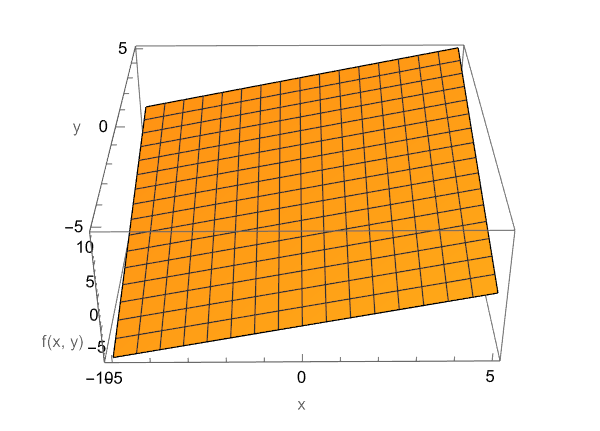
\includegraphics[width=0.7\linewidth]{Images/x+y}
			\caption{$f(x,y)=x+y$}
			\label{fig:xy}
		\end{figure}
		Let's see how the bivariate function $f(x, y) = x + y$ is related to the univariate functions $f(x) = x$ and $f(y) = y$.
		
		When we fix the value of $y$, say $y = y_0$, the function $f(x, y)$ becomes a univariate function in $x$: $f(x, y_0) = x + y_0$. This is essentially a vertical translation of the function $f(x) = x$ by a distance of $y_0$. In the 3D graph, this is represented by a line parallel to the $xz$-plane.
		Similarly, when we fix the value of $x$, say $x = x_0$, the function $f(x, y)$ becomes a univariate function in $y$: $f(x_0, y) = x_0 + y$. This is a vertical translation of the function $f(y) = y$ by a distance of $x_0$. In the 3D graph, this is represented by a line parallel to the $yz$-plane.
		When $y = 0$, $f(x, 0) = x$, which is the graph of the function $f(x) = x$. In the 3D graph, this is a line on the $xy$-plane.
		When $x = 0$, $f(0, y) = y$, which is the graph of the function $f(y) = y$. In the 3D graph, this is also a line on the $xy$-plane.
		The graphs of the functions $f(x) = x$ and $f(y) = y$ intersect on the $xy$-plane at the point $(0, 0)$, which corresponds to the point $(0, 0, 0)$ in the 3D graph.
		You can imagine that the graph of the function $f(x, y) = x + y$ is composed of countless lines parallel to the $xz$-plane and $yz$-plane, which correspond to the translations of $f(x) = x$ and $f(y) = y$ respectively. These lines form a plane in the 3D space.
		
		This plane can be seen as the result of translating $f(x) = x$ along the $y$-axis, or translating $f(y) = y$ along the $x$-axis. The combination of these two univariate functions in the 3D space forms the graph of the bivariate function $f(x, y) = x + y$.
	    \end{example}
	    
	    \begin{remark}
	    	Do not mix it up with function addition and multiplication earlier, because for the cases earlier, all functions are with respect to $x$, the same variable,
	    	while in this case a new variable is introduced.
	    \end{remark}
	    
	    
		We have worked out this example, however, here I'd like to give some extra knowledge on Cartesian product, especially its geometrical meaning. We just mentioned that two number set 
		will produce a set of ordered pairs with two elements, and in this case, we denote the set formed by Cartesian product of the same real number set as $\R^2$. Nevertheless, ordered pairs'
		elements are not always in pairs. We can even define an ordered pair of one single real number $(a)$, where $a \in \R$, or even three or more elements. We first examine $\R$ and $(a)$, 
		it is clear that $\R$ is just the set of real number that is already defined, while the ordered pair $(a)$ represents some $a\in \R$. Now we introduce another $b\in \R$ to
		form ordered pair $(a,b)$, and we have concluded that $(a,b) \in \R^2$. The process of developing $(a)$ to $(a,b)$,  is just creating a Cartesian product of real number set 
		to itself. To visualize this process, we need to find a suitable carrier for real number. We know that a real number could be infinitely huge or infinitely small, as there is no
		biggest or smallest real number (even though we haven't proven this, we just take it as common sense). We take some real number $-2 <r < 2$ as example. We can see that this interval is
		actually defined by a line on the Cartesian plane (or the Cartesian Coordinates). Since real number are infinite, so the whole set ordered pair $(a), a\in \R$, are defined in a line
		extending to both left and right-hand-side of the plane, giving us a whole line that extents forever.
		\begin{figure}[H]
			\centering
			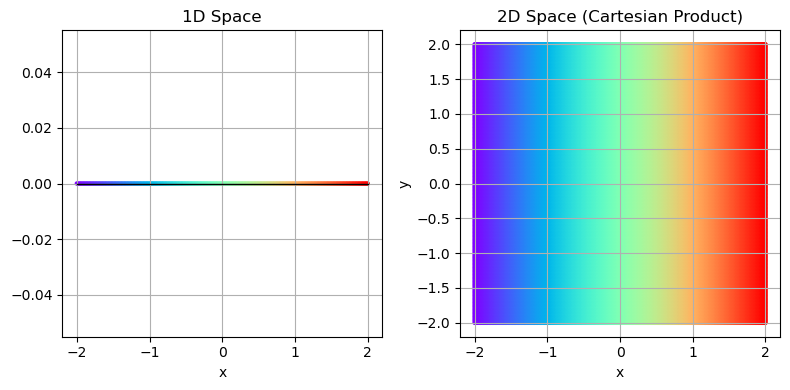
\includegraphics[width=0.8\linewidth]{Images/R^2}
			\caption{Visualization of $\R^1$ and $\R^2$}
			\label{fig:r2}
		\end{figure}
		Now we consider $(a,b)$, where both elements are from $\R$, so for the Cartesian products, we will get all possible combination of any $\R\times \R$. In this way, we can get a plane, just as
		shown in the graph. This is why call this system "Cartesian Coordinate". Naturally, we can also conclude that $\R^3 $ is a solid cubic in the 3D space.
		\begin{figure}[H]
			\centering
			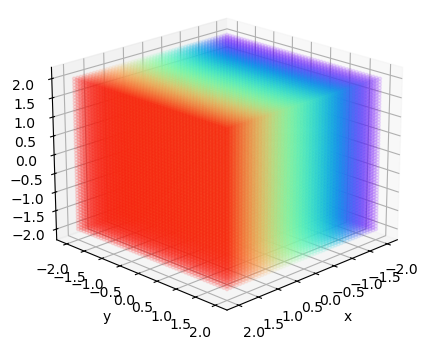
\includegraphics[width=0.7\linewidth]{Images/R^3}
			\caption[]{Visualization of $\R^3$}
			\label{fig:r3}
		\end{figure}
		But what about functions whose preimage are above $\R^3$? Sadly, there is no easy way to plot a function that are in 4D space, even though we can still use many techniques to analyze these
		high dimension functions, including function slicing. We will discuss $\R^n$ further in linear algebra and multivariable calculus. 
		
		Just now, we have somewhat shown another law about dimension or graphical representation of function.
		\begin{proposition}
			For any \textbf{n-variable function} with variables $x_1, x_2, \cdots, x_n$, for function $f(x_1,x_2,\cdots, x_n)$, ($x\in \R$), whose mapping is $\R \times \R \times \cdots \times \R = \R^n \to \R$.
			we need $n+1$ dimensions to plot a complete graph for the function. 
		\end{proposition}
		
		
		Additionally, $\R^n$ is defined as \textbf{The n-dimensional Euclidean Space}.
		\begin{definition}[The n-dimensional Euclidean Space]
		The n-dimensional Euclidean Space can be defined as the set of all real-valued functions defined on the index set $\{1, 2, \ldots, n\}$.
			\[\mathbb{R}^n = \{f \colon \{1, 2, \ldots, n\} \to \mathbb{R}\}\]
			
			where each function $f$ assigns a real number to each element of the index set $\{1, 2, \ldots, n\}$. We can represent these functions as n-tuples or vectors:
			
			\[f = (f(1), f(2), \ldots, f(n)) = (x_1, x_2, \ldots, x_n)\]
			
			where $x_i = f(i)$ for $i = 1, 2, \ldots, n$. Thus, each point in $\mathbb{R}^n$ can be identified with an n-tuple of real numbers $(x_1, x_2, \ldots, x_n)$.
			
			The set $\mathbb{R}^n$ is equipped with various algebraic and geometric structures, such as vector addition, scalar multiplication, and an inner product, which make it a real vector space of dimension $n$. Don't worry if you are confused by this, we will explore this topic further in linear algebra and other topics.
		\end{definition}
		
\subsection{Partial and Total Function}
Now we will introduce some ways to categorize functions. Earlier, we have discussed many functions where $f: \R \to \R$, but functions cannot always 
have a domain in a complete set. So we first introduce the idea of partial function.
\begin{definition}[Partial Function]
	A partial function from a set $A$ to a set $B$ is a function $f$ that satisfies the following conditions:
	\begin{enumerate}
		\item The domain of $f$, denoted by $\text{dom}(f)$, is a subset of $A$, i.e., $\text{dom}(f) \subseteq A$.
		\item For each $x \in \text{dom}(f)$, there is a unique $y \in B$ such that $f(x) = y$.
	\end{enumerate}
	
	In other words, a partial function is a function that may not be defined for all elements of its source set. Partial functions allow some input values to have no corresponding output values.
\end{definition}
\begin{example}
	Consider the function $f: \mathbb{R} \to \mathbb{R}$ defined as:
	$$
	f(x) = \begin{cases}
		\frac{1}{x}, & \text{if } x \neq 0 \\
		\text{undefined}, & \text{if } x = 0
	\end{cases}
	$$
	This function $f$ is a partial function because it is not defined for $x = 0$. The domain of $f$ is the set of all real numbers except zero, i.e., $\text{dom}(f) = \mathbb{R} \setminus {0}$.
\end{example}

By analogy, we can define total function as follows.
\begin{definition}[Total Function]
	A total function from a set $A$ to a set $B$ is a function $f$ that satisfies the following conditions:
	\begin{enumerate}
		\item The domain of $f$, denoted by $\text{dom}(f)$, is equal to $A$, i.e., $\text{dom}(f) = A$.
		\item For each $x \in A$, there is a unique $y \in B$ such that $f(x) = y$.
	\end{enumerate}
	
	In other words, a total function is a function that is defined for all elements of its source set. Every input value of a total function has a unique corresponding output value.
\end{definition}
\begin{example}
	Consider the function $g: \mathbb{R} \to \mathbb{R}$ defined as:
	$$
	g(x) = x^2
	$$
	
	This function $g$ is a total function because it is defined for all real numbers. The domain of $g$ is the entire set of real numbers, i.e., $\text{dom}(g) = \mathbb{R}$. For any input value $x \in \mathbb{R}$, the function $g$ assigns the unique output value $x^2$.
	
	A total function is a special case of a partial function where the domain is equal to the source set.
	
\end{example}

Another thing that worth discussing is that, earlier, we introduced function slicing that reduce the number of variable of a function. Function slicing has 
much to do with partial function.
\begin{proposition}[Function Slicing is Always a Partial Function]
	Function slicing is a technique that involves restricting the domain of a function to a specific subset. Given a function $f: A \to B$ and a subset $C \subseteq A$, the slice of $f$ over $C$, denoted by $f|_C$, is defined as:
	$$
	f|_C(x) = \begin{cases}
		f(x), & \text{if } x \in C \\
		\text{undefined}, & \text{if } x \notin C
	\end{cases}
	$$
	The function $f|_C$ has the same output values as $f$ for inputs in $C$, but it is undefined for inputs not in $C$.
	
	If the original function $f$ is a total function, then the slice $f|_C$ is a partial function, unless $C = A$. In the case where $C = A$, the slice $f|_C$ is the same as the original function $f$ and remains a total function.
	
	On the other hand, if the original function $f$ is already a partial function, then the slice $f|_C$ is also a partial function, regardless of the choice of $C$.
\end{proposition}







\subsection{Injective, Surjective, and Bijective Function}
We have known that functions are actually reflection from one set to the other set. We will look into several special mapping.

\begin{definition}[Injective Function]
    A function \( f: A \to B \) is called \emph{injective} (or \emph{one-to-one}) if every element of the codomain \( B \) is mapped by at most one element of the domain \( A \). For example, the function \( f(x) = 2x \) from \( \mathbb{R} \) to \( \mathbb{R} \) is injective because each value of \( f(x) \) is produced by exactly one value of \( x \).
\end{definition}

\begin{definition}[Surjective Function]
    A function is \emph{surjective} (or \emph{onto}) if every element of the codomain \( B \) is mapped by at least one element of the domain \( A \). For instance, the function \( g(x) = \sin(x) \) from \( \mathbb{R} \) to \( [-1, 1] \) is surjective because every value in \( [-1, 1] \) is the sine of some real number \( x \).
\end{definition}

\begin{definition}[Bijective Function]
    A function is \emph{bijective} if it is both injective and surjective, which means there is a perfect "pairing" between the sets: every element of \( A \) is paired with a unique element of \( B \), and every element of \( B \) is paired with a unique element of \( A \). An example of a bijective function is the identity function \( i(x) = x \) from \( \mathbb{R} \) to \( \mathbb{R} \).
\end{definition}

\begin{figure}[H]
    \centering
    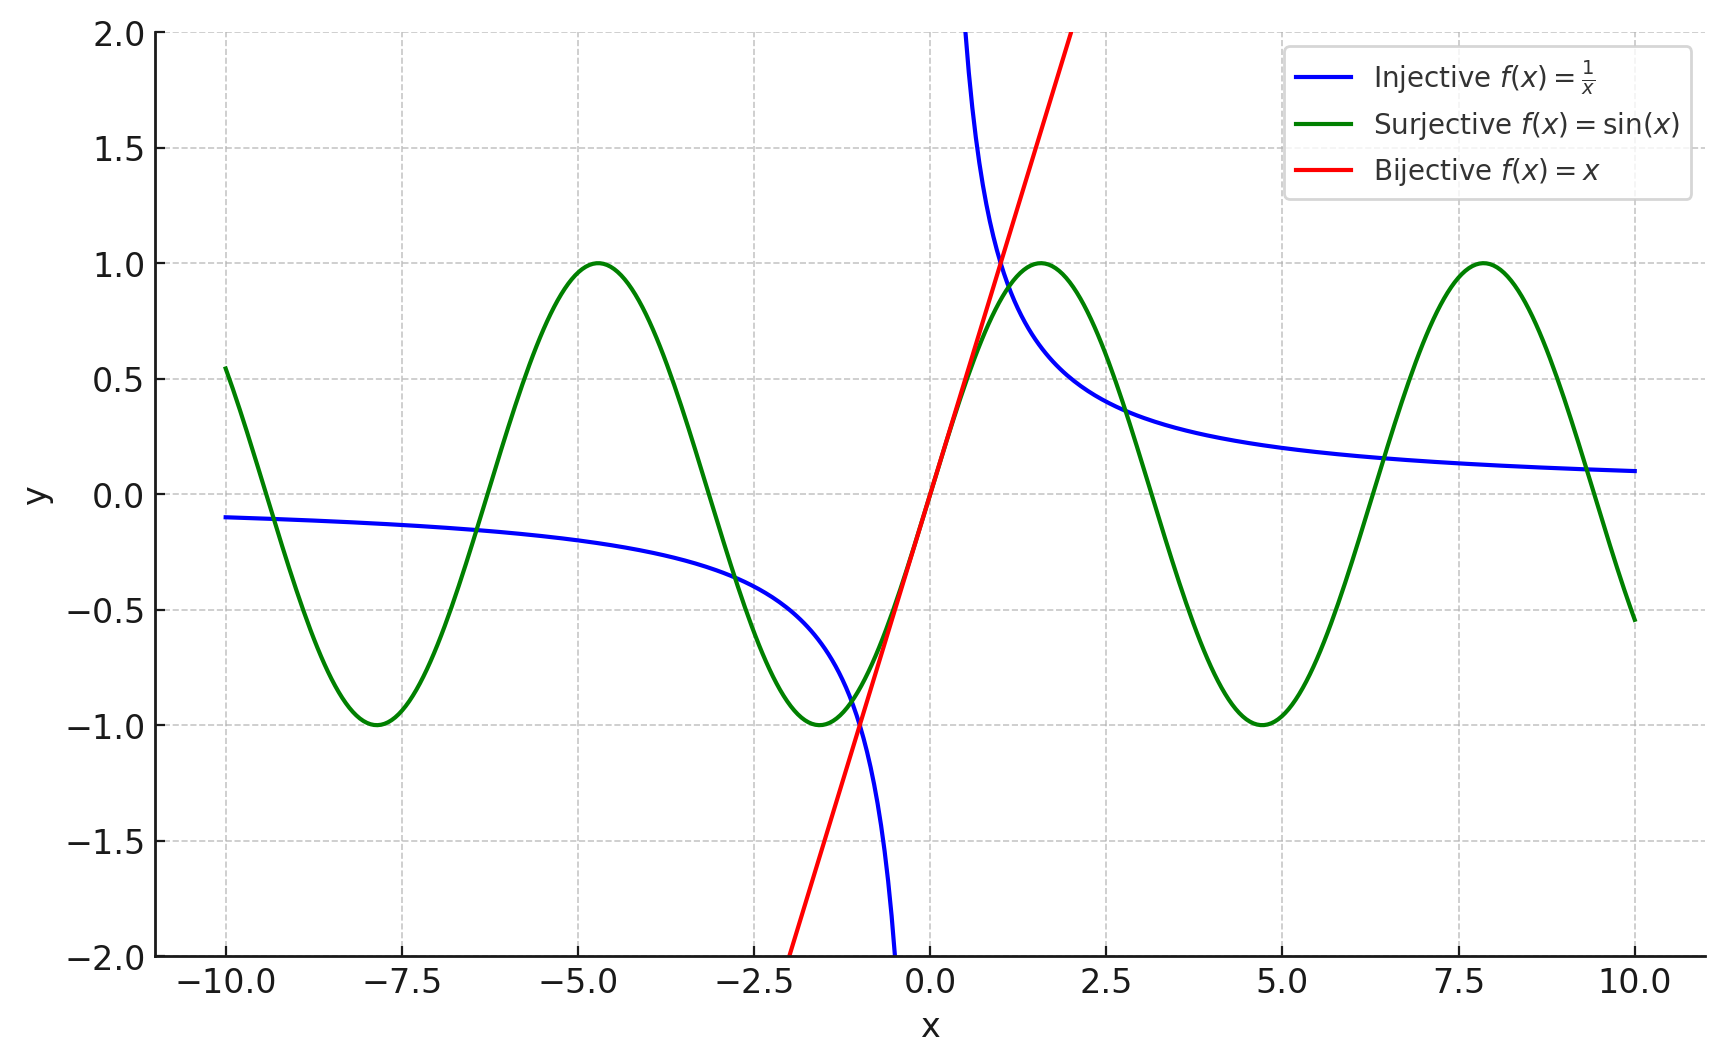
\includegraphics[width=0.75\linewidth]{Images/func.jpg}
    \caption{Examples of Special Mappings}
    \label{fig:fuc}
\end{figure}

Examine the figure \autoref{fig:fuc}, where one example of each type of function is shown. Fundamentally, when we define these functions, only two properties are involve:
\begin{itemize}
    \item A: It the mapping retrievable? (for every value in the image, we can find where it is from without any confusion.
    \item B: Is the mapping is full comparing to the preimage?(Whether every value in the preimage has a mapping to the image)
\end{itemize}
If A is satisfied, we call it injective function.

If B is satisfied, we call it surjective function.

If both A and B are satisfied, we say the function is bijective.

Using $A$, $B$, and $C$ to denote the set of injective, surjective, and bijective function respectively, it is therefore that :

    $$A\cap B = C$$

Which means that if a function is injective and surjective in the same time, it is bijective. 

Additionally, we need to distinguish bijective function with well-defined function.
\begin{definition}[Well-defined Function]
	A function \( f: A \rightarrow B \) is said to be \emph{well-defined} if for every element \( a \) 
	in the domain \( A \), there is a unique element \( b \) in the codomain \( B \) such that \( f(a) = b \). 
	This means that the function assigns exactly one output to each input. A well-defined function does not 
	assign multiple outputs to a single input, and every input for which the function is defined has an 
	output.
\end{definition}
\begin{remark}
	While all bijective functions are well-defined, not all well-defined functions are bijective. 
	Being well-defined is a minimal requirement for being a function at all. A well-defined function may 
	fail to be bijective if it is not injective, allowing different inputs to have the same output, or if 
	it is not surjective, meaning that some elements in the codomain do not correspond to any input from 
	the domain. Thus, while bijectivity implies a specific one-to-one correspondence between the entire 
	domain and codomain, well-definedness merely ensures that the function is consistently defined across 
	its domain.
\end{remark}
And these will be all we need to know about function for now, since the rest of the properties will be discussed in single-variable calculus. This section aims only introduce the idea of injectivity, surjectivity, and bijectivity.

\subsection{Exercises}

\begin{exercise}
	Let $f : \{0, 1\} \times \mathcal{P}(\mathbb{Z}) \to \mathbb{N}$ be a function. Which of the following correctly gives an example of an element from its domain and an element from its codomain?
	\begin{enumerate}
		\item $(8, -7)$ is an element of the domain and ${1, 9, 85}$ is an element of the codomain.
		\item $1$ is an element of the domain and ${6, 8}$ is an element of the codomain.
		\item ${0, 14}$ is an element of the domain and $19$ is an element of the codomain.
		\item $(1, \{-3, 6\})$ is an element of the domain and $9$ is an element of the codomain.
	\end{enumerate}
\end{exercise}
\begin{solution}
	Let's break down the domain and codomain of the function $f$:
	
	\begin{itemize}
		\item The domain of $f$ is ${0, 1} \times \mathcal{P}(\mathbb{Z})$, which means it consists of ordered pairs $(a, B)$, where $a$ is either $0$ or $1$, and $B$ is a subset of the set of integers $\mathbb{Z}$.
		\item The codomain of $f$ is $\mathbb{N}$, which is the set of natural numbers.
	\end{itemize}
	
	Now, let's examine each choice:
	
	\begin{enumerate}
		\item $(8, -7)$ is not an element of the domain because $8 \notin \{0, 1\}$, and $-7$ is not a subset of $\mathbb{Z}$. $\{1, 9, 85\}$ is a subset of $\mathbb{N}$, but not an element of $\mathbb{N}$.
		\item $1$ is an element of $\{0, 1\}$, but not an element of $\{0, 1\} \times \mathcal{P}(\mathbb{Z})$. $\{6, 8\}$ is a subset of $\mathbb{N}$, but not an element of $\mathbb{N}$.
		\item $\{0, 14\}$ is not an element of $\{0, 1\} \times \mathcal{P}(\mathbb{Z})$ because it is not an ordered pair. $19$ is an element of $\mathbb{N}$.
		\item $(1, \{-3, 6\})$ is an element of $\{0, 1\} \times \mathcal{P}(\mathbb{Z})$ because $1 \in \{0, 1\}$ and $\{-3, 6\} \subseteq \mathbb{Z}$. $9$ is an element of $\mathbb{N}$.
	\end{enumerate}
	
	Therefore, the correct answer is 4.
\end{solution}
\begin{exercise}
	Determine whether the rules below define functions from $\mathbb{R}$ to $\mathbb{R}$.
	\begin{enumerate}
		\item[a)] \( f(x) = 
		\begin{cases} 
		|x - 1| & \text{if } x < 4 \\
		|x| - 1 & \text{if } x > 2.
		\end{cases} \)
		
		\item[b)] \( f(x) = 
		\begin{cases} 
		|x - 1| & \text{if } x < 2 \\
		|x| - 1 & \text{if } x > -1.
		\end{cases} \)
		
		\item[c)] \( f(x) = 
		\begin{cases} 
		\frac{(x + 3)^2 - 9}{x} & \text{if } x \neq 0 \\
		6 & \text{if } x = 0.
		\end{cases} \)
		
		\item[d)] \( f(x) = 
		\begin{cases} 
		\frac{(x + 3)^2 - 9}{x} & \text{if } x > 0 \\
		x + 6 & \text{if } x < 7.
		\end{cases} \)
		
		\item[e)] \( f(x) = 
		\begin{cases} 
		\sqrt{x^2} & \text{if } x \geq 2 \\
		x & \text{if } 0 \leq x \leq 4 \\
		-x & \text{if } x < 0.
		\end{cases} \)
	\end{enumerate}
\end{exercise}
\begin{remark}
	You only need to check whether the domain covers the whole $\R$.
\end{remark}
\begin{exercise}
    Determine the images of the functions \( f: \mathbb{R} \rightarrow \mathbb{R} \) defined as follows:
    \begin{enumerate}
        \item[a)] \( f(x) = \frac{x^2}{1 + x^2} \).
        \item[b)] \( f(x) = \frac{x}{1 + |x|} \).
    \end{enumerate}
\end{exercise}
\begin{solution}
    We analyze the function \( f(x) = \frac{x^2}{1 + x^2} \):
    \begin{itemize}
        \item This function is defined for all \( x \in \mathbb{R} \).
        \item For \( x = 0 \), \( f(0) = 0 \).
        \item For \( x \neq 0 \), \( f(x) \) is always positive.
        \item As \( x \) approaches infinity, \( f(x) \) approaches 1.
    \end{itemize}
    Thus, the image of \( f \) is \( (0, 1] \).
    

    We analyze the function \( f(x) = \frac{x}{1 + |x|} \):
    \begin{itemize}
        \item This function is defined for all \( x \in \mathbb{R} \).
        \item For \( x > 0 \), as \( x \) increases, \( f(x) \) approaches 1.
        \item For \( x < 0 \), as \( x \) decreases, \( f(x) \) approaches -1.
    \end{itemize}
    Thus, the image of \( f \) is \( (-1, 1) \).
    \end{solution}

\begin{exercise}
	Let $f:\mathbb{Z}^+\times\mathbb{Z}^+\to\mathbb{Z}$ be the function defined by $f((a,b))=\gcd(a,b)+b$ where $\mathbb{Z}^+$ is the set of positive integers and $\gcd(a,b)$ is the greatest common divisor of $a$ and $b$.
	Is this a one-to-one (bijective) function? What is the image of the function?
\end{exercise}
\begin{solution}
	Take $(a_1, b_1) = (2, 2)$ and $(a_2, b_2) = (1, 3)$. Both $(2, 2)$ and $(1, 3)$ are elements of the domain $\mathbb{Z}^+ \times \mathbb{Z}^+$.
	
	Now, let's calculate $f((2, 2))$ and $f((1, 3))$:
	
	$f((2, 2)) = \gcd(2, 2) + 2 = 2 + 2 = 4$
	$f((1, 3)) = \gcd(1, 3) + 3 = 1 + 3 = 4$
	
	As we can see, $f((2, 2)) = f((1, 3)) = 4$, even though $(2, 2) \neq (1, 3)$. This demonstrates that $f$ is not one-to-one, as there exist distinct elements in the domain that map to the same element in the codomain.
	
	Now, let's determine the image of $f$. The image of a function is the set of all elements in the codomain that are mapped to by at least one element in the domain.
	
	Observe that for any $(a, b) \in \mathbb{Z}^+ \times \mathbb{Z}^+$:
	
	$\gcd(a, b) \geq 1$, because the greatest common divisor of two positive integers is always a positive integer.
	$b \geq 1$, because $b$ is a positive integer.
	Therefore, $f((a, b)) = \gcd(a, b) + b \geq 1 + 1 = 2$.
	
	This means that the smallest possible value of $f((a, b))$ is 2, and there is no upper limit on the value of $f((a, b))$ as $b$ can be arbitrarily large.
	
	Thus, the image of $f$ is the set ${x : x \in \mathbb{Z} \text{ and } x \geq 2}$, which is the set of all integers greater than or equal to 2.
	
	In conclusion, $f$ is not a one-to-one function, and its image is ${x : x \in \mathbb{Z} \text{ and } x \geq 2}$.
\end{solution}

\begin{exercise}
	Considering $X=\{1,2,3\}$ and $Y=\{a,b\}$. How to define a total function $f: X\to Y$?
	How many are there? List all the total functions. Also try to find the way to calculate
	the number of total functions obtained by $X$ and $Y$ with respect to $|X|, |Y|$.
\end{exercise}
\begin{solution}
	To obtain a total function, we must make sure that the preimage is exactly $X=\{1,2,3\}$, so we can pick which ever combinations of members of $Y$, so we have
	$(a, a, a)$,
	$(a, a, b)$,
	$(a, b, a)$,
	$(a, b, b)$,
	$(b, a, a)$,
	$(b, a, b)$,
	$(b, b, a)$,
	$(b, b, b)$.
	There are 8 total functions from $X$ to $Y$.
	 The number of total functions can be calculated using the formula $|Y|^{|X|}$, which in this case is $2^3 = 8$.
\end{solution}
\begin{exercise}
	Let $f$ and $g$ be the following functions.\\ $f:\mathcal{P}(\{1,2,3,4\})\to\mathcal{P}(\{1,2,3,4\})$ defined by $f(X)=\{1,2,3,4\}-X$.
	
	\noindent $g:\mathcal{P}(\{1,2,3,4\})\cdot\to\{0,1,2,3,4\}$ defined by $g(X)=|X|$.
	Discuss the existence of $f(f(x)), f(g(x)), g(f(x)), and g(g(x))$. If any
	of them exists, give a example.
\end{exercise}
\begin{solution}
	\textbf{1. $f(f(x))$:}
	$f(f(x))$ exists for all $x \in \mathcal{P}({1,2,3,4})$ because the codomain of $f$ is the same as its domain. This means that for any $x \subseteq {1,2,3,4}$, $f(x) \subseteq {1,2,3,4}$, so $f(f(x))$ is well-defined.
	
	Example:
	Let $x = {1,3}$. Then:
	\begin{align*}
		f(x) &= {1,2,3,4} - {1,3} = {2,4} \\
		f(f(x)) &= f({2,4}) = {1,2,3,4} - {2,4} = {1,3}
	\end{align*}
	
	\textbf{2. $f(g(x))$:}
	$f(g(x))$ does not exist because the codomain of $g$ is ${0,1,2,3,4}$, which is not a subset of the domain of $f$, $\mathcal{P}({1,2,3,4})$. Therefore, $g(x)$ is not a valid input for $f$.
	
	\textbf{3. $g(f(x))$:}
	$g(f(x))$ exists for all $x \in \mathcal{P}({1,2,3,4})$ because the codomain of $f$ is $\mathcal{P}({1,2,3,4})$, which is the domain of $g$. This means that for any $x \subseteq {1,2,3,4}$, $f(x) \subseteq {1,2,3,4}$, so $g(f(x))$ is well-defined.
	
	Example:
	Let $x = {2,3}$. Then:
	\begin{align*}
		f(x) &= {1,2,3,4} - {2,3} = {1,4} \\
		g(f(x)) &= g({1,4}) = |{1,4}| = 2
	\end{align*}
	
	\textbf{4. $g(g(x))$:}
	$g(g(x))$ does not exist because the codomain of $g$ is ${0,1,2,3,4}$, which is not a subset of the domain of $g$, $\mathcal{P}({1,2,3,4})$. Therefore, $g(x)$ is not a valid input for $g$.
	
	In summary, $f(f(x))$ and $g(f(x))$ exist for all $x \in \mathcal{P}({1,2,3,4})$, while $f(g(x))$ and $g(g(x))$ do not exist.
\end{solution}

\begin{exercise}
	We have discussed $\R^1$ to $\R^n$ in this section. Try to postulate that
	whether $R^0$ exists? If it exists, can it be defined by Cartesian Product.
	Try to prove your conclusion by deduction, and explain how can we visualize it, and
	is it necessary to visualize it in Cartesian Coordinate system.
	\begin{remark}
		Deduction is also known as "inverse induction".
	\end{remark}
\end{exercise}
\begin{proof}
	First, let's recall the definition of the Cartesian product for a finite collection of sets $A_1, A_2, \ldots, A_n$:
	
	\begin{align*}
		A_1 \times A_2 \times \cdots \times A_n = {(a_1, a_2, \ldots, a_n) \mid a_1 \in A_1, a_2 \in A_2, \ldots, a_n \in A_n}
	\end{align*}
	
	Now, consider the case where $n = 0$. We have an empty collection of sets, denoted by $\emptyset$. The Cartesian product of an empty collection of sets is defined as:
	
	\begin{align*}
		\prod_{i \in \emptyset} A_i = {()}
	\end{align*}
	
	This is a singleton set containing the empty tuple $()$. The empty tuple is a tuple with no components and is denoted by $()$.
	
	By definition, $\mathbb{R}^n$ is the Cartesian product of $n$ copies of $\mathbb{R}$:
	
	\begin{align*}
		\mathbb{R}^n = \underbrace{\mathbb{R} \times \mathbb{R} \times \cdots \times \mathbb{R}}_{n \text{ times}}
	\end{align*}
	
	When $n = 0$, we have:
	
	\begin{align*}
		\mathbb{R}^0 = \prod_{i \in \emptyset} \mathbb{R} = {()}
	\end{align*}
	
	Therefore, $\mathbb{R}^0$ exists and is equal to the singleton set containing the empty tuple $()$.
	
	\textbf{Visualization:}
	As mentioned earlier, visualizing $\mathbb{R}^0$ is not necessary, as it is a singleton set containing only the empty tuple. However, if we were to visualize it, it would be represented by a single point in a 0-dimensional space.
	
	In the Cartesian coordinate system, $\mathbb{R}^1$ is represented by a line, $\mathbb{R}^2$ by a plane, and $\mathbb{R}^3$ by a 3-dimensional space. As the dimension increases, the visualization becomes more complex. For $\mathbb{R}^0$, there are no axes to represent it in the Cartesian coordinate system, as it is a 0-dimensional space.
	
	\textbf{Conclusion:}
	$\mathbb{R}^0$ exists and can be defined as the Cartesian product of zero copies of $\mathbb{R}$, resulting in a singleton set containing the empty tuple $()$. While it is not necessary to visualize $\mathbb{R}^0$ in the Cartesian coordinate system, it can be thought of as a single point in a 0-dimensional space.
\end{proof}

\begin{exercise}
	If $f:A\to B$ and $g:B\to C$ are bijections (both injections and surjections), prove that 
	$g\circ f:A\to C$ is also a bijection.
\end{exercise}
\begin{proof}
	We aim to prove that the composition of two bijective functions is also a bijection.

	Let \(f: A \to B\) and \(g: B \to C\) be bijections. We need to show that \(g \circ f: A \to C\) is both an injection and a surjection.

	Assume \(x_1, x_2 \in A\) and \(g(f(x_1)) = g(f(x_2))\). Since \(g\) is an injection, if \(g(y_1) = g(y_2)\) then \(y_1 = y_2\) for any \(y_1, y_2 \in B\), which implies \(f(x_1) = f(x_2)\). Furthermore, since \(f\) is also an injection, \(x_1 = x_2\). Hence, \(g \circ f\) is an injection.

	Let \(z \in C\). Since \(g\) is a surjection, there exists \(y \in B\) such that \(g(y) = z\). Similarly, since \(f\) is a surjection, there exists \(x \in A\) such that \(f(x) = y\). Therefore, for \(z \in C\), there exists \(x \in A\) such that \(g(f(x)) = z\). Thus, \(g \circ f\) is a surjection.

	Combining both, we conclude that \(g \circ f\) is a bijection.
\end{proof}

\begin{exercise}
	is the inverse proposition of last statement true, if so prove it.
\end{exercise}
\begin{proof}
	We can use proof by contradiction here.\\
	Suppose that $g: A\to B$ and $f: B\to C, $ so that $f\circ g: A\to C$ . We will prove that if 
	$f\circ g$ is one-to-one, then $g$ is also one-to-one, so not only is the answer to the question “yes”. 
	Suppose that $g$ were not one-to-one. By definition this means that there are distinct elements 
	$a_1$ and $a_2$ in $A$ such that $g( a_1) = g( a_2) .$ Then certainly $f(g(a_1))=f(g(a_2))$, which is 
	the same statement as $(f\circ g)(a_1)=(f\circ g)(a_2).$ By definition this means that $f\circ g$ is not
	one-to-one, and our proof is complete.

\end{proof}
\begin{exercise}
	Let \( f \) be a function with domain \( \mathcal{D} \) and \( f(S) = \{ f(x) : x \in S \} \) for any subset \( S \) of \( \mathcal{D} \). Suppose \( C \) and \( D \) are subsets of \( \mathcal{D} \).
\begin{enumerate}
    \item[a)] Prove that \( f(C \cup D) \subseteq f(C) \cup f(D) \).
    \item[b)] Give an example where equality does not hold in part (a).
\end{enumerate}
\end{exercise}
\begin{solution}
	Below is solution for a).
	\begin{proof}
		Take any element \( y \in f(C \cup D) \). By definition of \( f(S) \), there exists an 
		\( x \in C \cup D \) such that \( f(x) = y \). Since \( x \) is in the union \( C \cup D \), 
		\( x \) must be in either \( C \) or \( D \). If \( x \in C \), then \( y = f(x) \in f(C) \). 
		Similarly, if \( x \in D \), then \( y = f(x) \in f(D) \). Therefore, in either case, 
		\( y \in f(C) \cup f(D) \), proving that \( f(C \cup D) \subseteq f(C) \cup f(D) \).
	\end{proof}
	Below is an example that the inequality holds.
	\begin{align*}
		f: \mathbb{R} \to \mathbb{R}, \quad f(x) &= x^2 \\
		C &= \{-1, 1\} \\
		D &= \{0, 2\} \\
		f(C) &= \{f(x) \mid x \in C\} = \{1\} \\
		f(D) &= \{f(x) \mid x \in D\} = \{0, 4\} \\
		f(C) \cup f(D) &= \{0, 1, 4\} \\
		f(C \cup D) &= \{f(x) \mid x \in C \cup D\} = \{0, 1, 4, 9\} \\
		\therefore f(C \cup D) &\neq f(C) \cup f(D)
	\end{align*}
	The equality does not hold when the function f is not injective,
	meaning that it maps distinct elements in the domain to the same element in the codomain. 
\end{solution}

\begin{exercise}
	Determine whether \( f: \mathbb{Z} \times \mathbb{Z} \rightarrow \mathbb{Z} \) is onto if
	\begin{enumerate}[label=(\alph*)]
		\item \( f(m, n) = 2m - n. \)
		\item \( f(m, n) = m^2 - n^2. \)
		\item \( f(m, n) = m + n + 1. \)
		\item \( f(m, n) = |m| - |n|. \)
		\item \( f(m, n) = m^2 - 4. \)
	\end{enumerate}
	\end{exercise}
	
	\begin{solution} 
	\begin{enumerate}[label=(\alph*)]
		\item This is clearly onto, since \( f(0, -n) = n \) for every integer \( n \).
		\item This is not onto, since, for example, \( 2 \) is not in the range. To see this, if \( m^2 - n^2 = (m - n)(m + n) = 2 \), then \( m \) and \( n \) must have the same parity (both even or both odd). In either case, both \( m - n \) and \( m + n \) are then even, so this expression is divisible by 4 and hence cannot equal 2.
		\item This is clearly onto, since \( f(0, n - 1) = n \) for every integer \( n \).
		\item This is onto. To achieve negative values we set \( m = 0 \), and to achieve nonnegative values we set \( n = 0 \).
		\item This is not onto, for the same reason as in part (b). In fact, the range here is clearly a subset of the range in that part.
	\end{enumerate}
	\end{solution}

	\begin{exercise}
		Let \( f \) be a function from the set \( A \) to the set \( B \). Let \( S \) and \( T \) be subsets of \( A \). Show that
		\begin{enumerate}[label=(\alph*)]
			\item \( f(S \cup T) = f(S) \cup f(T) \).
			\item \( f(S \cap T) \subseteq f(S) \cap f(T) \).
		\end{enumerate}
		\end{exercise}
		
		\begin{solution}
		\begin{enumerate}[label=(\alph*)]
			\item We need to show two inclusions:
			\begin{itemize}
				\item Suppose \( b \in f(S \cup T) \). This implies \( b = f(a) \) for some \( a \in S \cup T \). Thus, \( a \in S \) or \( a \in T \), and consequently, \( b \in f(S) \) or \( b \in f(T) \). Hence, \( b \in f(S) \cup f(T) \).
				
				\item Conversely, assume \( b \in f(S) \cup f(T) \). Then either \( b \in f(S) \) or \( b \in f(T) \), which means there exists an \( a \in S \) or \( a \in T \) such that \( b = f(a) \). Thus, \( a \in S \cup T \) and \( b \in f(S \cup T) \).
			\end{itemize}
			This shows that \( f(S \cup T) = f(S) \cup f(T) \), completing the proof.
		
			\item To prove the subset relation:
			\begin{itemize}
				\item Let \( b \in f(S \cap T) \). Then \( b = f(a) \) for some \( a \in S \cap T \). This means \( a \in S \) and \( a \in T \), hence \( b \in f(S) \) and \( b \in f(T) \). Therefore, \( b \in f(S) \cap f(T) \).
			\end{itemize}
			This establishes that \( f(S \cap T) \subseteq f(S) \cap f(T) \), as desired.
		\end{enumerate}
		\end{solution}

		\begin{exercise}
			Show that a partial function from \( A \) to \( B \) can be viewed as a function \( f^* \) from \( A \) to \( B \cup \{u\} \), where \( u \) is not an element of \( B \) and
			\[
			f^*(a) = 
			\begin{cases} 
			f(a) & \text{if } a \text{ belongs to the domain of definition of } f \\
			u & \text{if } f \text{ is undefined at } a.
			\end{cases}
			\]
			\end{exercise}
			
			\begin{solution}
			To show that a partial function \( f \) from \( A \) to \( B \) can be extended to a total function \( f^* \) from \( A \) to \( B \cup \{u\} \), we need to verify that for every element \( a \) in \( A \), the function \( f^* \) assigns exactly one element in \( B \cup \{u\} \).
			
			Consider any element \( a \) in \( A \). There are two possibilities:
			
			\begin{enumerate}
				\item If \( a \) is in the domain of definition of \( f \), then by the definition of \( f \), there is an associated element \( f(a) \) in \( B \). In this case, we define \( f^*(a) = f(a) \). Since \( f(a) \) is an element of \( B \), and \( B \) is a subset of \( B \cup \{u\} \), \( f^*(a) \) is an element of \( B \cup \{u\} \).
				
				\item If \( a \) is not in the domain of \( f \), which means \( f \) is undefined at \( a \), we assign a special element \( u \) that is not in \( B \) to \( a \). Specifically, we define \( f^*(a) = u \). By the choice of \( u \), we ensure that \( f^*(a) \) is in \( B \cup \{u\} \).
			\end{enumerate}
			
			In both cases, \( f^*(a) \) is a well-defined element of \( B \cup \{u\} \). Furthermore, the definition of \( f^* \) is such that each \( a \) in \( A \) is associated with exactly one element in \( B \cup \{u\} \), making \( f^* \) a total function. Therefore, \( f^* \) satisfies the definition of a function and extends \( f \) to the entire set \( A \) by assigning \( u \) where \( f \) is undefined.
			
			Thus, every partial function \( f: A \rightarrow B \) can indeed be considered a total function \( f^*: A \rightarrow B \cup \{u\} \) with the addition of a special element \( u \) to handle the undefined cases in \( f \).
			\end{solution}

			\begin{remark}
				The extension of a partial function \( f: A \rightarrow B \) to a total function \( f^*: A \rightarrow B \cup \{u\} \) relates closely to the concept of function slicing presented in Proposition 2.2 of the book. Function slicing involves restricting the domain of a function to a subset \( C \subseteq A \), whereas extending a partial function involves expanding the codomain to include an element \( u \) that handles undefined cases.
				
				In essence, slicing a total function can create a partial function \( f|_C \) which is only defined for inputs in subset \( C \). Extending a partial function \( f \) to \( f^* \) can be viewed as reversing this process, by adding an element to the codomain for the undefined cases, thereby making it total. 
				
				The slice \( f|_C \) has the same output values as \( f \) for inputs in \( C \), and is undefined for inputs not in \( C \). Similarly, \( f^* \) maintains the output values of \( f \) for inputs where \( f \) is defined and assigns the value \( u \) for inputs where \( f \) is not defined. Both processes — slicing and extending — are techniques to manipulate the domain and codomain of functions to achieve desired properties of partiality or totality.
			\end{remark}			
%------------------------------------------------
\section{Summation}
Before we move on to the most important part of this chapter, sequence, we use this section to introduce a prerequisite for studying its properties. We introduce the Sigma sign.

In earlier chapters, we have seen exercises such as finding the expression of the sum of the first nth positive integer:
$$1 + 2 + \dots + (n-1) + (n)= \frac{n(n+1)}{2}$$ 
From now on, we will use the sigma notation to deal with the summation of numbers. Such as:
\subsection{Sigma Notation}
\begin{notation}[Sigma Notation]
    \[
\sum_{i=1}^{n} i = \frac{n(n + 1)}{2}
    \]
\end{notation}
Where $i$ is quite similar to iterator, or sometimes we also call counter in programming languages, and $n$ refers to the condition of termination. The expression right after the sigma sign is called \textbf{summand}.

Actually, this is not the only way to express summation, it is also equivalent to:
\[\sum_{1\leq i\leq n} i = \frac{n(n+1)}{2}\]

Also, like what we do for set, we can also write sigma notation using description, such as: 
\[
\sum_{1 \leq k \leq 100} k^2
\]

\( k \) is odd

\subsection{Properties and Techniques of Sigma Notation}
This part of the section shows how we can handle summation expressions.
One of the greatest convenience of sigma notation is that every expression is adjustable, we can change the variable as what we prefer as in the following example.
\begin{example} \label{exp:siginvariance}
 \[
\sum_{1 \leq k \leq n} a_k = \sum_{1 \leq k+1 \leq n} a_{k+1}
\]
\end{example}
This technique has a significant effect to some mathematical proofs.
Another points to keep in mind is that: always make the expression simple in terms of upper and lower boundary.
\begin{example}
    Examine this expression: 
    \[\sum_{k=0}^{n} k(k-1)(k-n)\]
    The sum when k equals to 0, 1, and $n$ is 0. In this case we cannot say it is a good expression, as what we want is the sum it self, while 0 does not matter for us. Therefore, we just fine-tune it to:
    \[\sum_{k=2}^{n-1} k(k-1)(k-n)\]
    This makes it concise and clear.
\end{example}

\subsubsection{Manipulation of Sigma Notation}
For a set \( K \), the following summation properties hold. Let \( c \) be a constant, and \( a_k \), \( b_k \) be sequences indexed by \( K \):

\begin{equation}
    \sum_{k \in K} c a_k = c \sum_{k \in K} a_k \quad \text{(Distributive Law)}
    \label{eq:constant_factor}
\end{equation}

\begin{equation}
    \sum_{k \in K} (a_k + b_k) = \sum_{k \in K} a_k + \sum_{k \in K} b_k \quad \text{(Associative Law)}
    \label{eq:summation_of_sums}
\end{equation}

\begin{equation}
    \sum_{k \in K} a_k = \sum_{p(k) \in K} a_{p(k)} \quad \text{(Commutative Law, as in example \autoref{exp:siginvariance})} 
    \label{eq:permutation_invariance}
\end{equation}
The proof is attached below.

\textbf{Proof of Constant Factor Law:}

Let \( c \) be a constant and \( a_k \) be a sequence indexed by a finite set \( K \). We want to show that \( \sum_{k \in K} c a_k = c \sum_{k \in K} a_k \).

By the definition of summation and the distributive property of multiplication over addition, we have:
\begin{equation}
    \sum_{k \in K} c a_k = c a_1 + c a_2 + \ldots + c a_n = c (a_1 + a_2 + \ldots + a_n) = c \sum_{k \in K} a_k.
\end{equation}
This concludes the proof of the constant factor law.

\textbf{Proof of Summation of Sums Law:}

Let \( a_k \) and \( b_k \) be sequences indexed by a finite set \( K \). We want to show that \( \sum_{k \in K} (a_k + b_k) = \sum_{k \in K} a_k + \sum_{k \in K} b_k \).

By the definition of summation and the associative and commutative properties of addition, we have:
\begin{equation}
    \begin{split}
\sum_{k \in K} (a_k + b_k) &= (a_1 + b_1) + (a_2 + b_2) + \ldots + (a_n + b_n) \\
&= (a_1 + a_2 + \ldots + a_n) + (b_1 + b_2 + \ldots + b_n) \\
&= \sum_{k \in K} a_k + \sum_{k \in K} b_k
\end{split}
\label{eq:sum_of_sums}
\end{equation}
This concludes the proof of the summation of sums law.

\textbf{Proof of Permutation Invariance Law:}

Let \( a_k \) be a sequence indexed by a finite set \( K \). Let \( p: K \to K \) be a bijection, which means \( p \) permutes the indices. We want to show that \( \sum_{k \in K} a_k = \sum_{p(k) \in K} a_{p(k)} \).

By the definition of summation and the fact that addition is commutative (the order does not matter), we have:
\begin{equation}
    \sum_{k \in K} a_k = a_1 + a_2 + \ldots + a_n = a_{p(1)} + a_{p(2)} + \ldots + a_{p(n)} = \sum_{p(k) \in K} a_{p(k)}.
\end{equation}
This concludes the proof of the permutation invariance law.
\subsubsection{Multiple Sums}
Sometimes we use sigma notation with multiple variables, just like what we can do to write loops in programming languages.

    
$$\sum_{1 \leq j, k \leq 3} a_j b_k = a_1b_1 + a_1b_2 + a_1b_3 + a_2b_1 + a_2b_2 + a_2b_3 + a_3b_1 + a_3b_2 + a_3b_3 $$


In the context of summation, we often encounter a situation where a sum is taken over a set of pairs. Specifically, let \( P(j, k) \) be a property involving the indices \( j \) and \( k \), and \( a_{j,k} \) be elements corresponding to these indices. The summation over all pairs \( (j, k) \) satisfying property \( P \) is equivalent to summing over all indices separately:

\[
\sum_{P(j,k)} a_{j,k} = \sum_{j,k} a_{j,k} \cdot P(j,k).
\]

This notation serves as a shorthand for expressing the sum over a subset of indices determined by the property \( P \).
There are also cases where we must use two sigma notation in the same time.

 
\begin{example}[Double Summation]
    When considering a double sum over a set of pairs, we often come across the following identity:

\begin{equation}
\sum_{j}\sum_{k} a_{j,k} [P(j,k)]
\end{equation}

where \( [P(j,k)] \) is an Iverson bracket which equals 1 if the property \( P \) holds for the pair \( (j,k) \) and 0 otherwise.
\end{example}


By interchanging the order of summation, we observe that:

\begin{equation}
\sum_{j}\sum_{k} a_{j,k} [P(j,k)] = \sum_{k}\sum_{j} a_{j,k} [P(j,k)].
\end{equation}

This property allows us to switch the order of summation without changing the result, which can be particularly useful in various mathematical analyzes.

Double summation could also be used to simplify a given summation.
Considering the expression at the beginning of this section:
$$\sum_{1 \leq j, k \leq 3} a_j b_k = a_1b_1 + a_1b_2 + a_1b_3 + a_2b_1 + a_2b_2 + a_2b_3 + a_3b_1 + a_3b_2 + a_3b_3 $$

\begin{example}[Converting to Double Summation]
    \[
\sum_{1 \leq i,j,k \leq 3} a_j b_k = \sum_{\substack{i,j,k \\ 1 \leq i,j,k \leq 3}} a_j b_k \left[1 \leq j \leq 3\right] \left[1 \leq k \leq 3\right]
\]
\[
= \sum_j \sum_k a_j b_k \left[1 \leq j \leq 3\right] \left[1 \leq k \leq 3\right]
\]
\[
= \sum_j a_j \left[1 \leq j \leq 3\right] \sum_k b_k \left[1 \leq k \leq 3\right]
\]
\[
= \sum_j a_j \left[1 \leq j \leq 3\right] \left( \sum_k b_k \left[1 \leq k \leq 3\right] \right)
\]
\[
= \left( \sum_j a_j \left[1 \leq j \leq 3\right] \right) \left( \sum_k b_k \left[1 \leq k \leq 3\right] \right)
\]
\[
= \left( \sum_{j=1}^3 a_j \right) \left( \sum_{k=1}^3 b_k \right).
    \]

\end{example}
To explicit:
In the situation where we perform the same range of summation over each variable, the first two lines' triple summation is:
\[
(a_1b_1 + a_1b_2 + a_1b_3) + (a_2b_1 + a_2b_2 + a_2b_3) + (a_3b_1 + a_3b_2 + a_3b_3).
\]
Utilizing the distributive property to combine the summation operations into one involving \( a \), since \( a \) and each \( k \) for \( 1 \leq j \leq 3 \) are independent, yields (as in the third line):
\[
a_1(b_1 + b_2 + b_3) + a_2(b_1 + b_2 + b_3) + a_3(b_1 + b_2 + b_3).
\]

Consider a double sum over two independent indices, if the indices are independent, the summation of the product can be split into the product of two summations. For instance, the sum of products of \(a_j\) and \(b_k\) over \(j\) in \(J\) and \(k\) in \(K\) can be expressed as: \( (a_1 + a_2 + a_3)(b_1 + b_2 + b_3) \). This can be generalized to an expression:

\begin{equation}
\sum_{j \in J} \sum_{k \in K} a_j b_k = \left( \sum_{j \in J} a_j \right) \left( \sum_{k \in K} b_k \right),
\end{equation}
which is known as the \textbf{general distributive law}.
\begin{remark}
    If you are an agile reader, you must have noticed that this expression is a kind of representation of Cartesian sets in algebra. The general distributive law allows the sum over a function of elements from the Cartesian product of two sets to be expressed as the product of sums over each set if the function is separable into independent factors.
\end{remark}
\subsection{Exercises}
\begin{exercise}
    Express the triple sum
\[
\sum_{1 \leq i < j < k \leq 4} a_{ijk}
\]
as a three-fold summation (with three \(\sum\)'s), 

\begin{enumerate}[label=\alph*.]
    \item summing first on \( k \), then \( j \), then \( i \);
    \item summing first on \( i \), then \( j \), then \( k \).
\end{enumerate}
Also write your triple sums out in full without the \(\sum\)-notation, using parentheses to show what is being added together first.
\end{exercise}
\textbf{Solution:}

\textbf{(a)} \[
\sum_{i=1}^{4} \sum_{j=i+1}^{4} \sum_{k=j+1}^{4} a_{ijk} = 
\sum_{i=1}^{2} \sum_{j=i+1}^{3} \sum_{k=j+1}^{4} a_{ijk} = 
((a_{123} + a_{124}) + a_{134}) + a_{234}.
\]

\textbf{(b)} \[
\sum_{k=1}^{4} \sum_{j=1}^{k-1} \sum_{i=1}^{j-1} a_{ijk} = 
\sum_{k=3}^{4} \sum_{j=2}^{k-1} \sum_{i=1}^{j-1} a_{ijk} = 
a_{123} + (a_{124} + a_{134} + a_{234}).
\]

\begin{exercise}
    Demonstrate your understanding of \(\Sigma\)-notation by writing out the sums
\[
\sum_{k=0}^{5} a_k \quad \text{and} \quad \sum_{0\leq k^2 \leq 5} a_{k^2}
\]
in full. (Watch out—the second sum is a bit tricky.)

\end{exercise}
\textbf{Solution:}

The first sum is:
\[
a_0 + a_1 + a_2 + a_3 + a_4 + a_5
\]

The second sum,  $k \in \{-2, -1, 0, 1, 2\}$, therefore:
\[
a_4 + a_1 + a_0 + a_1 + a_4
\]

\begin{exercise}
    The general rule for summation by parts is equivalent to
\[
\sum_{0 \leq k < n} (a_{k+1} - a_k)b_k = a_nb_n - a_0b_0 - \sum_{0 \leq k < n} a_{k+1}(b_{k+1} - b_k), \quad \text{for } n \geq 0.
\]

Prove this formula by using the distributive, associative, and commutative laws.
\end{exercise}
Hint: Use Associative Law to LHS, try to make the indices of the two sums as similar as possible.
\begin{proof}
    \begin{align*}
        \text{LHS} &= \sum_{0\leq k < n} a_k b_{k+1} - \sum_{0\leq k < n} a_k b_k \\
        &= \sum_{0\leq k < n} a_k b_{k+1} - \sum_{-1\leq k < n-1} a_{k+1} b_{k+1} \\
        &= \sum_{0\leq k < n} a_k b_{k+1} - \sum_{0\leq k < n-1} a_{k+1} b_{k+1} \\
        &= \sum_{k=0}^{n-1} a_k b_{k+1} - \sum_{k=0}^{n-2} a_{k+1} b_{k+1} \\
        &= a_n b_{n-1} - a_0 b_0 + \sum_{k=0}^{n-2} a_k b_k - \sum_{k=0}^{n-2} a_{k+1} b_{k+1} \\
        &= a_n b_{n-1} - a_0 b_0 + \sum_{0\leq k < n-1} a_k (b_k - b_{k+1}) \\
        &= a_n (b_n - b_{n-1}) + a_n b_{n-1} - a_0 b_0 - \sum_{0\leq k < n-1} a_{k+1} (b_{k+1} - b_k) \\
        &= a_n (b_n - b_{n-1} + b_{n-1}) - a_0 b_0 - \sum_{0\leq k < n} a_{k+1} (b_{k+1} - b_k) \\
        &= a_n b_n - a_0 b_0 - \sum_{0\leq k < n} a_{k+1} (b_{k+1} - b_k) \\
        &= \text{RHS}
        \end{align*}
\end{proof}
\begin{exercise}
    Is the following expression correct or not? Give your reason.
    \[
\left( \sum_{i=1}^{n} a_i \right) \left( \sum_{j=1}^{n} \frac{1}{a_j} \right) = \sum_{1 \leq i \leq n} \sum_{1 \leq j \leq n} \frac{a_i}{a_j} = \sum_{1 \leq i \leq n} \sum_{1 \leq i \leq n} \frac{a_i}{a_i} = \sum_{i=1}^{n} 1 = n
\]
\end{exercise}
\textbf{Solution:}

Consider the expression given by:
\[
\left( \sum_{i=1}^{n} a_i \right) \left( \sum_{j=1}^{n} \frac{1}{a_j} \right)
\]
and its expansion into a double sum:
\[
\sum_{1 \leq i \leq n} \sum_{1 \leq j \leq n} \frac{a_i}{a_j}
\]

It is claimed that this is equal to:
\[
\sum_{1 \leq i \leq n} \sum_{1 \leq i \leq n} \frac{a_i}{a_i} = \sum_{i=1}^{n} 1 = n
\]

However, this claim overlooks the fact that the double sum includes terms where \( i \neq j \), which are not necessarily equal to 1. Only when \( i = j \) does the term \( \frac{a_i}{a_j} \) simplify to 1, contributing to the count of \( n \).

Hence, the proper expansion of the double sum should be written as:
\[
\sum_{i=1}^{n} \sum_{j=1}^{n} \frac{a_i}{a_j} = \sum_{i=1}^{n} 1 + \sum_{\substack{i,j=1 \\ i \neq j}}^{n} \frac{a_i}{a_j}
\]
where the first sum on the right-hand side counts the \( n \) instances where \( i = j \), and the second sum accounts for the \( n(n-1) \) instances where \( i \neq j \).

The claim would only be true if all \( a_i \) are equal, which is a special case, not the general case. In the general case, the expression evaluates to something different from \( n \) due to the presence of terms where \( i \neq j \). 

Therefore, the original statement is incorrect unless the condition that all \( a_i \) are equal is specified.

\begin{exercise}
    Consider the following double summation where $a_i, a_j, b_i, b_j \in \mathbb{R}$.
    $$\sum_{i=1}^{n} \sum_{j=1}^{n} (a_ib_j-a_jb_i)$$
    $$\sum_{i=1}^{n} \sum_{j=1}^{n} (a_ib_j-a_jb_i)^2$$
    Is there anything special about these expressions? Manage to find all the equivalent expressions of
    the sum of squares in sigma notation. Also consider, if the order of summand increases to infinity, 
    whether these properties still exist?
\end{exercise}
\textbf{Solutions:}

For $\sum_{i=1}^{n} \sum_{j=1}^{n} (a_ib_j-a_jb_i)$
\begin{itemize}
    \item It could be seen that the sums are actually symmetrical. When $i=j$, $a_ib_j-a_jb_i=0$.
    \item If you list several of the first nth term, the term with indices $(i, j)$ will be canceled by $(j, i)$ term, since $(a_ib_j-a_jb_i)+(a_jb_i-a_ib_j)=0$ 
\end{itemize} 
We can visualize it in a matrix with $n=5$.
\begin{figure}[H]
    \centering
    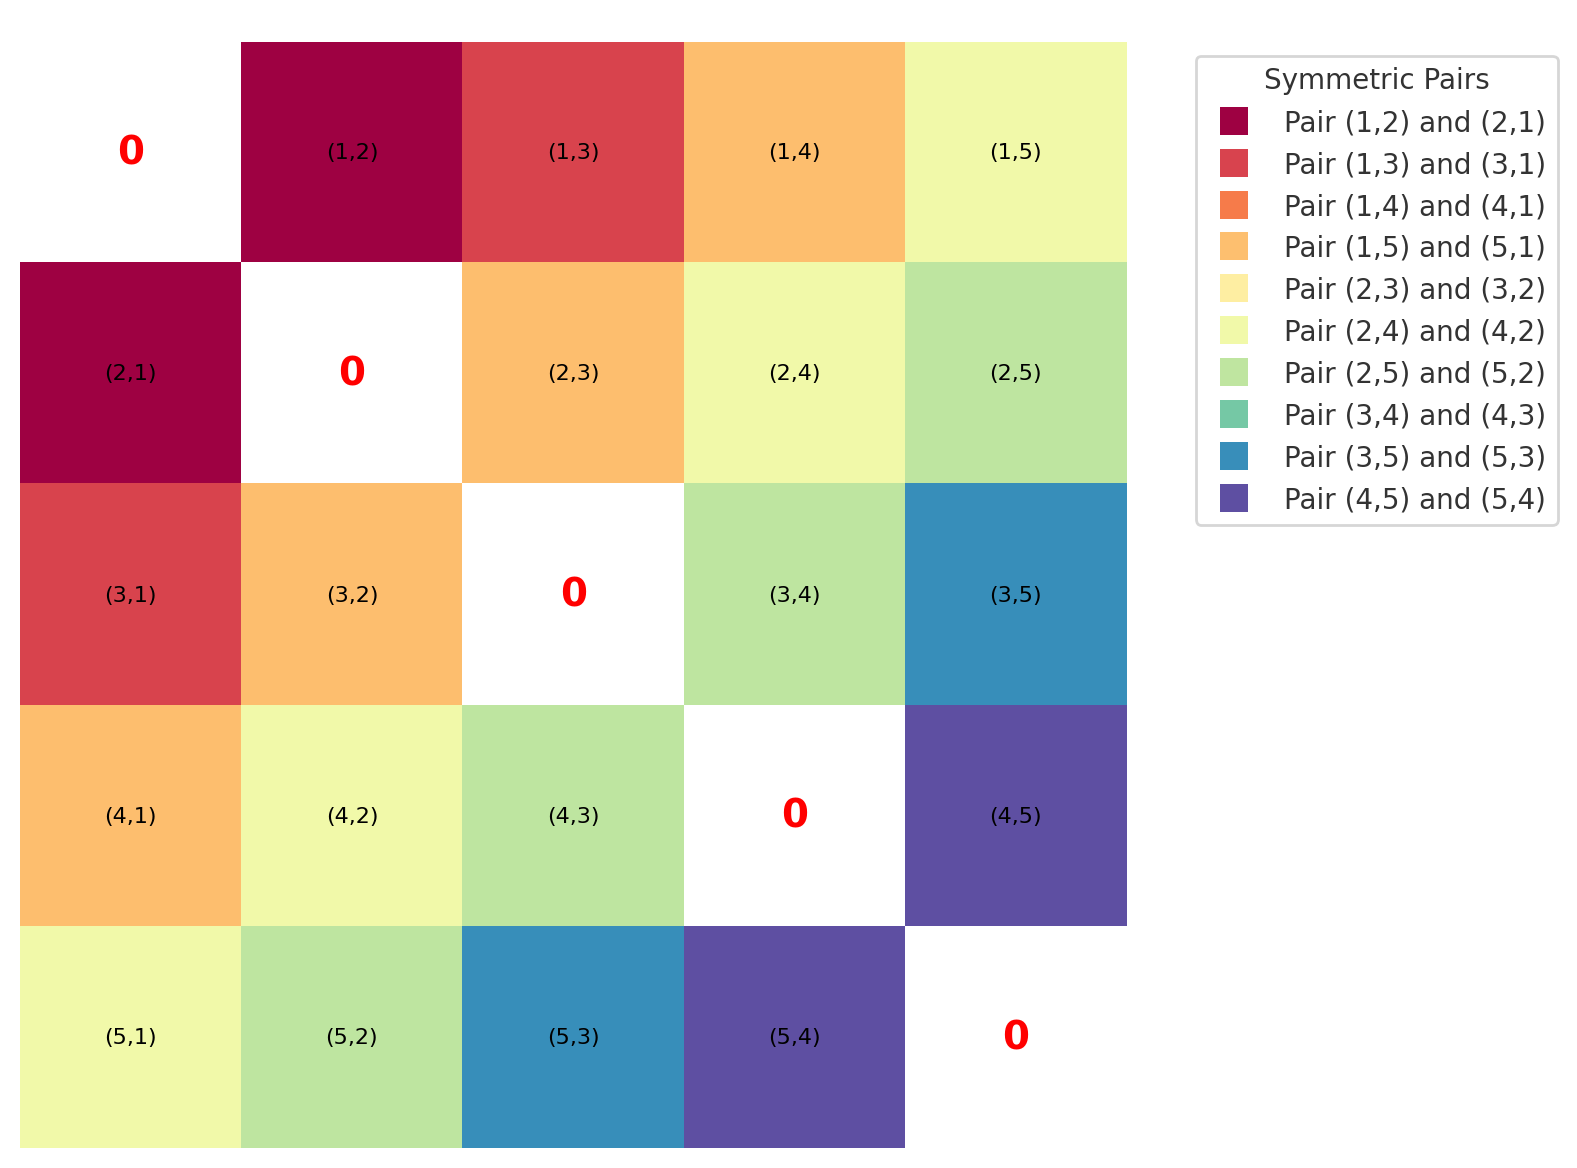
\includegraphics[width = 0.8\textwidth]{mtxvis.png}
    \caption{Visualization of $\sum_{i=1}^{n} \sum_{j=1}^{n} (a_ib_j-a_jb_i)$}
\end{figure}

With this image, we expand it until n; we can still cancel all elements symmetrical by the diagonal on by one. As the sum on the diagonal is 0, we conclude that 
$$\sum_{i=1}^{n} \sum_{j=1}^{n} (a_ib_j-a_jb_i)=0$$

Now consider the summation of squares. $(a_ib_j-a_jb_i)^2 = 0$ still holds for  $i=j$, but what about the symmetrical pairs $(i, j)$ and $(j, i)$?
We can figure it out by analysis by expanding the square of sum.
$$\sum_{i=1}^{n} \sum_{j=1}^{n}\left(a_{i}^{2} b_{j}^{2}-2 a_{i} a_{j} b_{i} b_{j}+a_{j}^{2} b_{i}^{2}\right)$$
By associative property of summation, we rearrange it as:
$$\sum_{i=1}^{n} \sum_{j=1}^{n}(a_i^2 b_j^2+a_j^2b_i^2) - 2\sum_{i=1}^{n} \sum_{j=1}^{n}a_ia_jb_ib_j$$
When $i \neq j$, each pair of $(i, j)$ and $(j, i)$. The sum of symmetric pair is
$$(a_i^2 b_j^2+a_j^2b_i^2 - 2a_ia_jb_ib_j) + (a_j^2 b_i^2+a_i^2b_j^2 - 2a_ia_jb_ib_j)$$
Rearrange it as:
$$2(a_i^2 b_j^2+a_j^2b_i^2) - 4(a_ia_jb_ib_j)$$
Still, as the sum of $(i, j)$ terms where $i=j$ is 0. We can ignore the diagonal. Hence, we have $n/2$ pairs
of $(a_i^2 b_j^2+a_j^2b_i^2) - 4(a_ia_jb_ib_j)$. This could be written as:
$$\frac{1}{2} \sum_{i=1}^{n} \sum_{j=1}^{n}2[(a_i^2 b_j^2+a_j^2b_i^2) - 4(a_ia_jb_ib_j)]$$
$$\sum_{i=1}^{n} \sum_{j=1}^{n}[(a_i^2 b_j^2+a_j^2b_i^2) - 2(a_ia_jb_ib_j)]$$
Notice that, $\sum_{i=1}^{n} \sum_{j=1}^{n}a_i^2 b_j^2 = \sum_{i=1}^{n} \sum_{j=1}^{n}a_j^2b_i^2$ due to the
diagonal symmetry of the summation as illustrated in the graph. We are adding the same term twice. 
Hence, we have:
$$2\sum_{i=1}^{n} \sum_{j=1}^{n}[a_i^2 b_j^2 - (a_ia_jb_ib_j)]$$
We can further simplify it by rule out the terms where $i=j$, as the summand is 0 in those cases.
We rewrite the sum as:
$$2\sum_{i=1}^{n-1} \sum_{j=2}^{n} [a_i^2 b_j^2 - (a_ia_jb_ib_j)]$$
or in single summation, we have:
$$2\sum_{i \neq j}[a_i^2 b_j^2 - (a_ia_jb_ib_j)] = 2\sum_{1 \leq i < j \leq n}[a_i^2 b_j^2 - (a_ia_jb_ib_j)] $$

For $\sum_{i=1}^{n} \sum_{j=1}^{n} (a_ib_j-a_jb_i)^n$, the symmetric property of summand still exists.
However we cannot prove it for now, as we need to use polynomial theorem to be introduced in Combinatorics.

%------------------------------------------------

\section{Sequence}
If everything so far is not a problem for you, congratulations, because you have known everything you need to know sequence. Sequence is an important concept that will be used throughout your journey of learning math. A Sequence
is defined as:
\begin{definition}
    A sequence is a function \( f: \mathbb{N} \to \mathbb{R} \), where \(\mathbb{N}\) is the set of natural numbers and \(\mathbb{R}\) is the set of real numbers. The value \( f(n) \) 
    is the \( n \)-th term of the sequence, often denoted as \( a_n \). Therefore, a sequence can be represented as \( \{a_n\}_{n=1}^{\infty} \) for an infinite sequence or \( \{a_n\}_{n=1}^{N} \) for a finite sequence of length \( N \).
\end{definition} 

\subsection{Introduction}
Sequences could be either infinite or finite. A \textit{sequence} is defined to be a function \( S \) whose domain \( D \) is a nonempty interval of integers. \( S \) is an \textit{infinite sequence} if \( D \) has the form \( \{a..\} \). % Usually \( a \) is 1 or 0.

\( S \) is a \textit{finite sequence} if \( D \) has the form \( \{a..b\} \) where \( a \leq b \). When \( |D| = n \), we will say that \( S \) is an \( n\text{-sequence} \). We will take the domain of an \( n\text{-sequence} \) to be the set \( \{1..n\} \). % But \( a \) could be 0, and then \( D \) is \( \{0..(n - 1)\} \).

The (natural) ordering of the domain of a sequence \( S \) gives a natural ordering to the ordered pairs in the set \( S \). If \( S \) is a 5-sequence, then
\[ S = \{(1, S(1)), (2, S(2)), (3, S(3)), (4, S(4)), (5, S(5))\} \]

\begin{example}
    Suppose \( D = \{1..10\} \), and we define the function \( S \) on \( D \) by

\[ S(i) = \text{the smallest prime factor of the integer } (1 + i). \]

Then \( D \) is a finite interval of integers, and so \( S \) is the sequence denoted by

\[ S = (2, 3, 2, 5, 2, 7, 2, 3, 2, 11). \]
\end{example}

\begin{definition}[Sum of Sequence]
    If \( S = (S_1, S_2, S_3, \ldots, S_n) \) is a finite sequence of numbers, the corresponding \textit{series} is the sum of the entries in \( S \)
    is:

\[ S_1 + S_2 + S_3 + \ldots + S_n. \]
\end{definition}
\subsection{Special Sequences}
This section introduces common sequences as well as their properties.
\subsubsection{Algorithmic Sequence}
Algorithmic sequences are a fundamental concept in both computer science and mathematics, forming the backbone of algorithm design and analysis. These sequences are typically defined as an ordered set of steps or instructions, aimed at solving a specific problem or accomplishing a particular computation.
\begin{definition}[Arithmetic Sequence]
    An arithmetic sequence of the form
\[
a, a + d, a + 2d, \ldots, a + nd, \ldots
\]
where the initial term \( a \) and the common difference \( d \) are real numbers.
\end{definition}
Usually, the notation $a_n$ is used to express the nth term of a sequence (starting from 0). For the example in the 
definition, we have $a_0 = a$ and $a_n = a_0 + nd$. 
We also have:
$$a_1 = a_0 + d$$
$$a_2 = a_1 + d$$
$$\dots$$
$$a_n = a_0 + nd$$ 
for $n>=1$, $n\in \mathbb{Z}$:
$$a_n = a_{n-1} + d$$
These formula shows the linking between consecutive terms in an arithmetic sequence. We know that the sum
$s$ of the sequence is:
\begin{align*}
    S & =\ a_{0} \ +\ a_1\ \ +\ \dotsc \ +\ a\_n\\
    S & =\ a_{0} \ +\ a_{0} +d\ +\ \dotsc \ +\ a_{n-1} +d
    \end{align*}
The sum is expressed in infinite terms, and it is called \textbf{open form equation}. Accordingly, there are also \textbf{closed form
equations}.
\begin{definition}[Open Form]
    An \textit{open form} or \textit{non-closed form} expression, on the other hand, does not have a finite standard representation and often requires recursive or iterative methods for evaluation. It may involve summations, integrals, or other operations that are not easily simplified into a finite number of operations.
\end{definition}
\begin{definition}[Closed Form]
    A \textit{closed form} expression is a mathematical expression that can be evaluated in a finite number of standard operations. It typically involves constants, variables, and operations from algebra, calculus, and other areas of mathematics that can be computed in a finite number of steps.
    A closed form expression provides a direct way to compute the term of a sequence without the need for recursion.
\end{definition}

Is the open form good for calculating the sum of a sequence? Suppose now I want to know $S_{100}$ (The sum of the first 100th terms),
with the open form, I still have to calculate 99 terms using the definition of this sequence. So is there a way 
to make it possible that we get the sum in one step? Think about closed form. The closed form allows us to calculate
the sum directly. But is it possible to transform an open expression to closed form? If possible, how?

You may already notice that the open form has a property of infinity, and each step is somewhat related.
Isn't it a perfect problem to be solved by mathematical induction? We will leave this proof as a exercise, and here we provide another direct proof
by the symmetry of arithmetic sequence.
\begin{theorem}[Sum of Arithmetic Sequence]
    For  arithmetic sequence \( a_0, a_1, \ldots, a_{n-1} \), where each term can be expressed as \( a_i = a_0 + id \) and \( d \) is the common difference. The sum of the first nth terms is:
    \[ S = \frac{n}{2}[2a_0 + (n-1)d] \] or \[ S = \frac{n}{2}(a_0 + a_{n-1}) \] where \[ a_n = a_0 + nd \]
\end{theorem}
\begin{remark}
    We are trying to find the sum of the first n terms, and the first term is $a_0$, so the last term is
    $a_{n-1}$.
\end{remark}
\begin{proof}
    Consider an arithmetic sequence \( a_0, a_1, \ldots, a_n \), where each term can be expressed as \( a_i = a_0 + id \) and \( d \) is the common difference.
    \item Write the sum of the sequence in order:
\[
S = a_0 + (a_0 + d) + (a_0 + 2d) + \ldots + (a_0 + (n-1)d)
\]

\item Write the sum of the sequence in reverse order:
\[
S = (a_0 + (n-1)d) + (a_0 + (n-2)d) + \ldots + a_0
\]

\item Add these two equations together, every pair of terms within the brackets forms: \[ 2a_0 + (n-1)d \]

\item Since each term appears in a pair, there are \( n \) such pairs.

\item The resulting equation is \( 2S = n[2a_0 + (n-1)d] \).

\item Solving for \( S \) gives us \( S = \frac{n}{2}[2a_0 + (n-1)d] \) or \( S = \frac{n}{2}(a_0 + a_n) \), where \( a_n = a_0 + (n-1)d \).
\end{proof}


\subsubsection{Geometric Sequence}
Geometric sequence is the other important and common sequence that involved in problem-solving of computer
Science. 
A geometric sequence, also known as a geometric progression, is a sequence of numbers where each term after 
the first is found by multiplying the previous term by a fixed, non-zero number called the common ratio. 
Mathematically, a geometric sequence is defined as follows:
\begin{definition}[Geometric Sequence]
    Given the first term \( a_0 \) (also referred to as \( a_1 \) in some texts) and the common ratio \( r \), the \( n \)-th term of a geometric sequence \( a_n \) can be expressed as:
\[
a_n = a_0 \cdot r^n \quad \text{for } n \geq 0
\]
where \( n \) is a non-negative integer representing the position of the term in the sequence.
\end{definition}    

The common ratio \( r \) can be any real number. If \( |r| < 1 \), the terms of the sequence 
will get progressively smaller and approach zero. If \( |r| > 1 \), the terms will grow progressively 
larger. If \( r = 1 \), the sequence is constant, and if \( r = -1 \), the sequence will alternate 
between two values.

We can deduce the sum of a specific geometric sequence by direct proof.
\begin{theorem}[Sum of Geometric Sequence]
    
\end{theorem}

\begin{proof}
    Consider a geometric sequence with the first term \( a_0 \) and the common ratio \( r \) where \( r \neq 1 \). The sequence is given by:
\[ a_0, a_0r, a_0r^2, \ldots, a_0r^{n-1} \]

The sum of the first \( n \) terms of the sequence, denoted by \( S_n \), is:
\[ S_n = a_0 + a_0r + a_0r^2 + \ldots + a_0r^{n-1} \]

To find a formula for \( S_n \), multiply the entire sequence by \( r \):
\[ rS_n = a_0r + a_0r^2 + a_0r^3 + \ldots + a_0r^n \]

Subtract the original sum \( S_n \) from this new sum \( rS_n \) to get a telescoping series:
\[ rS_n - S_n = a_0r^n - a_0 \]

Solving for \( S_n \) gives us:
\[ S_n = \frac{a_0(1 - r^n)}{1 - r} = \]

This is the sum formula for the first \( n \) terms of a geometric sequence when \( r \neq 1 \). If \( r = 1 \), the sequence is constant, and the sum of the first \( n \) terms is simply \( n \) times the first term \( a_0 \).
\end{proof}
%----------------------------------------------------------------------
\subsubsection{characteristic Sequence}
\begin{definition}[Characteristic Sequence]
    Suppose that \( U \) is some given \( n \)-set whose elements have been \textit{indexed} (listed in a certain order) so that \( U = \{x_1, x_2, \ldots, x_n\} \). If \( A \) is a subset of \( U \), the \textit{characteristic sequence} of \( A \) is the function whose domain is \( \{1..n\} \) defined by

\[
X^A_i = X^A(i) = 
\begin{cases} 
1 & \text{if } x_i \in A \\
0 & \text{if } x_i \notin A 
\end{cases}
\]
\end{definition}

\begin{example}
    If \( U \) is the set of the first 10 odd positive integers, \( A \) is the subset of primes in \( U \), and \( B \) is the set of multiples of 3 in \( U \), then
    
    \[
    \begin{aligned}
    &U = \{1, 3, 5, 7, 9, 11, 13, 15, 17, 19\} &&// x_i = 2i - 1. \\
    &A = \{3, 5, 7, 11, 13, 17, 19\} \\
    &B = \{3, 9, 15\} \\
    &X^A = (0, 1, 1, 1, 0, 1, 1, 0, 1, 1) \\
    &X^B = (0, 1, 0, 0, 1, 0, 0, 1, 0, 0).
    \end{aligned}
    \]
    \end{example}

    Characteristic sequences may be used as an implementation model for subsets of any given indexed set \( U \). The set operations may be done on these sequences:
    \[
    X^{A \cap B}_i = X^A_i \times X^B_i;
    \]
    \[
    X^{A \cup B}_i = X^A_i + X^B_i - X^A_i \times X^B_i;
    \]
    \[
    X^{A \setminus B}_i = X^A_i - X^A_i \times X^B_i.
    \]
    
    If \( A \subseteq B \) then
    \[
    X^A_i \leq X^B_i \quad \text{for each index } i,
    \]
    and
    \[
    |A| = \sum_{i=1}^{n} X^A_i.
    \]

%----------------------------------------------------------------------
\subsection{Exercises}
\begin{exercise}
    Find the sum of arithmetic sequence using mathematical induction. Try \textbf{NOT} use the conclusion in this section.
\end{exercise}
Hint: Consider the sum of the first nth positive integer. Try to make assumption by taking it as an arithmetic sequence.
\begin{proof}
    Let \( S(n) \) denote the sum of the first \( n \) terms of an arithmetic sequence with the first term \( a_0 \) and common difference \( d \).
    \begin{itemize}
        \item \textbf{Base Case (\( n = 1 \))}: The sum of the sequence with only the first term is the first term itself, \( S(1) = a_0 \).
        \item \textbf{Inductive Step}: Assume that the sum of the first \( k \) terms \( S(k) \) is given by a certain formula. We want to show that the sum of the first \( k+1 \) terms \( S(k+1) \) can be expressed using the same formula.
        \end{itemize}
        
        For the base case, we can easily see that:
        \[
        S(1) = a_0
        \]
        As $\sum_{1}^{n}i = \frac{n(n+1)}{2}$, which could be taken as an arithmetic sequence with $a_0=1$ and
        $a_n=n$.
        By this, assume that the sum of the first \( k \) terms is:
        \[
        S(k) = \frac{k}{2} [a_0 + a_n]
        \]
        equivalent to
        \[
        S(k) = \frac{k}{2} [2a_0 + (k-1)d]
        \]
        
        To prove the inductive step for \( S(k+1) \), consider:
        \[
        S(k+1) = S(k) + a_0 + kd
        \]
        
        Substituting the inductive hypothesis into the above equation yields:
        \[
        S(k+1) = \frac{k}{2} [2a_0 + (k-1)d] + a_0 + kd
        \]
        
        After simplifying, we aim to show that:
        \[
        S(k+1) = \frac{k+1}{2} [2a_0 + kd]
        \]
        
        This will complete the proof if we can establish that the simplified version of \( S(k+1) \) matches the form of the inductive hypothesis.
\end{proof}
\begin{exercise}
    Prove the sum of geometric sequence  is \( S_n = \frac{a_0(1 - r^n)}{1 - r} = \) using mathematical induction.
\end{exercise}
\begin{proof}
    We want to prove that the sum of the first \( n \) terms of a geometric sequence \( S_n \) with the first term \( a \) and common ratio \( r \) (where \( r \neq 1 \)) is given by:

\[ S_n = \frac{a(1 - r^n)}{1 - r} \]

\textbf{Base Case (n=1):}

The sum of the first term is simply the term itself:

\[ S_1 = a \]

which agrees with the formula.

\textbf{Inductive Step:}

Assume the formula holds for \( n = k \), that is,

\[ S_k = \frac{a(1 - r^k)}{1 - r} \]

We need to prove that it also holds for \( n = k+1 \):

\[ S_{k+1} = \frac{a(1 - r^{k+1})}{1 - r} \]

Starting with the inductive hypothesis for \( S_k \) and adding the \( (k+1) \)-th term \( ar^k \) to both sides, we have:

\[ S_k + ar^k = \frac{a(1 - r^k)}{1 - r} + ar^k \]

Simplifying, we obtain:

\[ S_{k+1} = S_k + ar^k = \frac{a - ar^{k+1}}{1 - r} \]

which is the same as the formula for \( S_{k+1} \), thus completing the proof.
\end{proof}
\begin{exercise}
    Given a sequence \( \{a_n\} \) and a series \( S_n = an^2 + bn + c (a \neq 0) \).

\begin{enumerate}
    \item Find the general term \( a_n \);
    \item Is the sequence \( \{a_n\} \) an arithmetic sequence?
\end{enumerate}
\end{exercise}
Hint: How can we get the value of a term from the sum of a sequence?
\textbf{Solution:}

\begin{enumerate}
    \item For \( n \geq 2 \), \( a_n = S_n - S_{n-1} = (an^2 + bn + c) - [a(n-1)^2 + b(n-1) + c] \) \\
    \( = (b+a) + (n-1) \cdot 2a \),
    
    Therefore, for \( n=1 \), \( a_1 = (b+a) + (1-1) \cdot 2a = b + a + c - S_1 \), \\
    and the general term is
    \[
    a_n = 
    \begin{cases}
        a + b + c & (n=1) \\
        (b+a) + (n-1) \cdot 2a & (n \geq 2)
    \end{cases}
    \]

    \item Since \( c = 0 \), \( a_n \) can be simplified to \( a_n = a + b \), which is constant and equals \( 2a \) when \( n \geq 2 \). This implies \( \{a_n\} \) is an arithmetic sequence with common difference \( 2a \), provided \( a, b \) are constants and \( a \neq 0 \).
    
    Note: From \( S_n \) we can deduce \( a_n = S_n - S_{n-1} \) when \( n \geq 2 \). Since \( a_1 = S_1 \), the sequence \( a_n = S_n - S_{n-1} \) (for \( n \geq 2 \)) and \( a_1 \) is the first term. The sequence \( \{a_n\} \) is an arithmetic sequence.
    
    Therefore, the general term \( a_n \) can be expressed as:
    \[
    a_n = 
    \begin{cases}
        S_1 & (n=1) \\
        S_n - S_{n-1} & (n \geq 2)
    \end{cases}
    \]
    
    Given the series \( \{a_n\} \) with \( S_n = an^2 + bm + c (a \neq 0) \), the sequence \( \{a_n\} \) is an arithmetic sequence with common difference \( 2a \) when \( c = 0 \).
\end{enumerate}

\begin{exercise}
    Given constants $a$, $b$, $c$, consider the sum $S_n = 1^2 + 2^2 + 3^2 + \ldots + n(n+1)^2 = \frac{n(n+1)}{12}(an^2 + bn + c)$, where $an^2 + bn + c \neq 0$.
\end{exercise}
\begin{proof}
    For $n=1$, we have $\frac{1}{6}(a+b+c)$, thus $a_1 = 4 = \frac{1}{6}(a+b+c)$.
For $n=2$, we have $\frac{22}{2} = 11 = \frac{1}{2}(4a+b+c)$, thus $a_2 = 22 = 9a + 3b + c$.
For $n=3$, $a_3 = 70 = 9a + 3b + c$.\\

From these equations, we find that:
\begin{align*}
    a + b + c &= 24 \\
    4a + b + c &= 44 \\
    9a + 3b + c &= 70
\end{align*}

Solving the system, we get $a=3$, $b=11$, $c=10$.
For \(n = 1, 2, 3\), the sum can be expressed as:
\[
1 \cdot 2^2 + 2 \cdot 3^2 + \ldots + n(n+1)^2 = \frac{n(n+1)}{12}(3n^2 + 11n + 10),
\]
thus, \(S_n = 1 \cdot 2^2 + 2 \cdot 3^2 + \ldots + n(n+1)^2\).

For a general term \(k\), \(S_k = \frac{k(k+1)}{12}(3k^2 + 11k + 10)\). Therefore,
\[
S_{k+1} = S_k + (k+1)(k+2)^2
\]
\[
= \frac{k(k+1)}{12}(3k^2 + 11k + 10) + (k+1)(k+2)^2
\]
\[
= \frac{k(k+1)}{12}((k+2)(3k+5) + (k+1)(k+2)^2)
\]
\[
= \frac{(k+1)(k+2)}{12}(3k^2 + 5k + 12k + 24)
\]
\[
= \frac{(k+1)(k+2)}{12}(3(k+1)^2 + 11(k+1) + 10).
\]

Hence, by induction, we can show that for \(n = k+1\) the sum is valid.

Finally, with \(a = 3\), \(b = 11\), \(c = 10\), we confirm that the given sequence is indeed a second-order arithmetic sequence.
\end{proof}

\begin{exercise}
    Evaluate:
    \begin{enumerate}
        \item $S = \sum_{1}^{n} \frac{N}{2^n}$
        \\
        \item $S = \sum_{1}^{n} \frac{3n-2}{5^{n-1}}$  
    \end{enumerate}
\end{exercise}

\textbf{Solution:}

(1) Given the series \( S_n = \frac{1}{2} + \frac{2}{4} + \frac{3}{8} + \cdots + \frac{n}{2^n} \), we can write:

\[
S_n - \frac{1}{2}S_n = \frac{1}{2} + \frac{1}{4} + \frac{1}{8} + \cdots + \frac{1}{2^n} - \frac{n}{2^{n+1}}
\]

This simplifies to:

\[
\frac{1}{2}S_n = \frac{1}{2} \left(1 - \left(\frac{1}{2}\right)^n\right) = \frac{1}{2} - \frac{1}{2^{n+1}} = \frac{1}{2} - \frac{n}{2^{n+1}} + \frac{n}{2^{n+1}}
\]

Hence, the series sum is:

\[
S_n = 2 - \frac{1}{2^{n-1}} - \frac{n}{2^n} = 2 - \frac{n+2}{2^n}
\]

(2) Considering the series \( S_n = 1 + \frac{4}{5} + \frac{7}{25} + \cdots + \frac{3n-2}{5^{n-1}} \), we proceed similarly:

\[
\left(1 - \frac{1}{5}\right)S_n = 1 + \frac{3}{5} + \frac{3}{25} + \cdots + \frac{3}{5^{n-1}} - \frac{3n-2}{5^n}
\]

The terms form a geometric series, so we get:

\[
S_n = 1 + \frac{3}{5} \left(1 + \frac{1}{5} + \frac{1}{25} + \cdots + \frac{1}{5^{n-2}}\right) - \frac{3n-2}{5^n}
\]

Applying the formula for the sum of a geometric series, we find:

\[
S_n = 1 + \frac{3}{5} \left(\frac{1 - \left(\frac{1}{5}\right)^{n-1}}{1 - \frac{1}{5}}\right) - \frac{3n-2}{5^n}
\]

Simplifying, we obtain:

\[
S_n = 1 + \frac{3}{5} \left(\frac{5^n - 5}{4 \cdot 5^{n-1}}\right) - \frac{3n-2}{5^n}
\]

Further simplification gives us:

\[
S_n = \frac{35}{16} - \frac{12n+7}{16 \cdot 5^{n-1}}
\]
%------------------------------------------------
\chapterimage{chap2.png} % Chapter heading image
\chapterspaceabove{5.75cm} % Whitespace from the top of the page to the chapter title on chapter pages
\chapterspacebelow{10cm} % Amount of vertical whitespace from the top margin to the start of the text on chapter pages
\chapter{Number System, Algorithm, and Recursion}

Computer Science is most commonly known as an engineering subject, while the unanimous pursuit of all engineering subjects are solving problems. This chapter delves in to methods to solve problems, which is also known as \textbf{algorithm}. In the world of Computer Science, everything is proceeded in a methodical manner, and the very dependency of this is algorithm. Meanwhile, we will introduce pseudocode, one of the most important tools for algorithm analysis, as well as the representation of number in Computer Science.

%------------------------------------------------

\section{Numbers}
Every reader could be quite surprised when seeing the title for this section. Yes, numbers, we have known what is number since the very beginning when we get to learn math as toddlers. In this section, we will explain the system of number, not only will we figure out how numbers and their operations are defined, but how they are categorized.
\subsection{Typology of Numbers}
This part recalls the type of numbers we've learned since primary school and their set notations.
\label{sec:number}
\begin{enumerate}
  \item \textbf{Natural Numbers}
  \begin{itemize}
    \item Definition: Natural numbers are the set of positive integers used for counting and ordering, which do not include zero or negative numbers.
    \item Set Notation:
    \[
    \mathbb{N} = \{1, 2, 3, \ldots\}
    \]
  \end{itemize}

  \item \textbf{Integers}
  \begin{itemize}
    \item Definition: Integers are all the whole numbers including positive natural numbers, their negatives, and zero.
    \item Set Notation:
    \[
    \mathbb{Z} = \{\ldots, -3, -2, -1, 0, 1, 2, 3, \ldots\}
    \]
  \end{itemize}

  \item \textbf{Rational Numbers}
  \begin{itemize}
    \item Definition: Rational numbers are numbers that can be expressed as the quotient of two integers, a fraction \( \frac{a}{b} \), where \( a \) and \( b \) are integers and \( b \neq 0 \). The set includes all integers and fractions.
    \item Set Notation:
    \[
    \mathbb{Q} = \left\{\frac{a}{b} \mid a, b \in \mathbb{Z}, b \neq 0\right\}
    \]
  \end{itemize}
\begin{remark}
    For numbers that are written in finite decimal places, if there is a looping part in the decimal places,
    it is still recoganized as rational numbers. For instance, $\frac{1}{3}$ could be repesented as $0.33333\dots$.
    Usually, we use upperline to mark the repeating part, in this case it is$0.\overline{3}$. But for those who
    have infinitely non-repeating decimal places, such as $\pi=3.1415926535\dots$, we categorize it as irrational number,
    as they cannot be written in the $\frac{a}{b}$ form.
\end{remark}
  \item \textbf{Irrational Numbers}
  \begin{itemize}
    \item Definition: Irrational numbers are real numbers that cannot be expressed as a ratio of two integers. The decimal expansion of irrational numbers is non-terminating and non-repeating. Examples include \(\pi\) and \(\sqrt{2}\).
    \item Set Notation:
    \[
    \mathbb{I} = \{x \in \mathbb{R} \mid x \notin \mathbb{Q}\}
    \]
    (Note: \(\mathbb{I}\) is used here for illustrative purposes and is not a standard symbol.)
  \end{itemize}

  \item \textbf{Real Numbers}
  \begin{itemize}
    \item Definition: The real numbers include both rational and irrational numbers, encompassing all points on an infinitely extended number line. The set of real numbers is continuous and is composed of all limits of sequences of rational numbers.
    \item Set Notation:
    \[
    \mathbb{R} = \{x \mid x \text{ is a limit of a sequence of rational numbers}\}
    \]
  \end{itemize}

  \item \textbf{Prime Numbers}
\begin{itemize}
  \item Definition: A prime number is a natural number greater than 1 that has no positive divisors other than 1 and itself. In other words, \( p \) is prime if \( p > 1 \) and if \( p \) is divisible only by 1 and \( p \).
  \item Set Notation:
  \[
  \mathbb{P} = \{p \in \mathbb{N} \mid p > 1 \text{ and } p \text{ has no divisors other than } 1 \text{ and } p\}
  \]
  \item Examples: The first few prime numbers are:
  \[
  2, 3, 5, 7, 11, 13, 17, \ldots
  \]
\end{itemize}
The following Venn diagram shows the relationship between different number sets.
\begin{figure}[H]
    \centering
    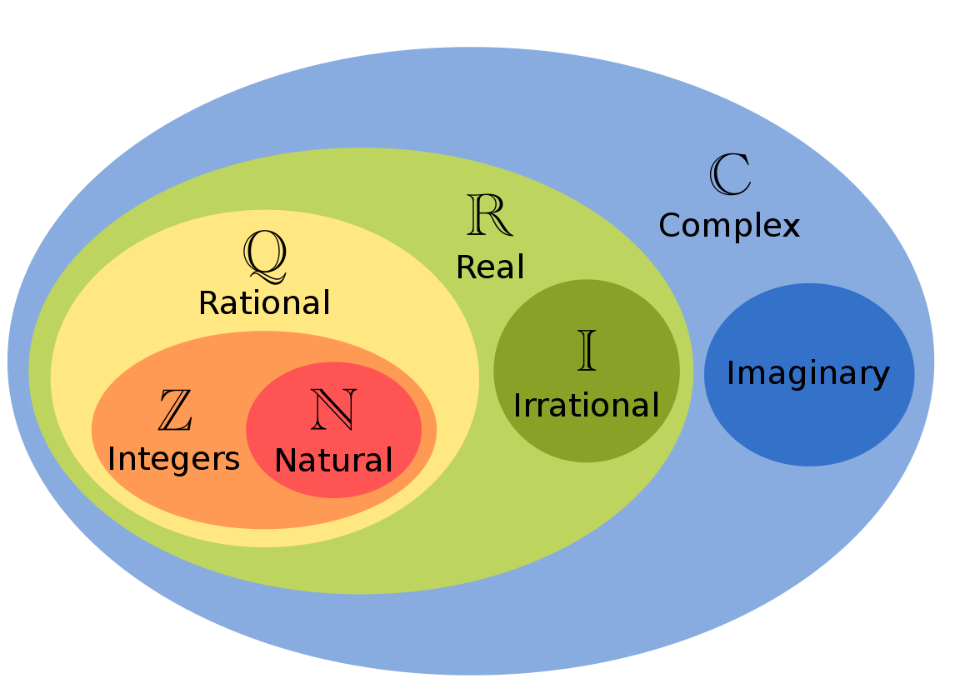
\includegraphics[width=0.5\linewidth]{venn.png}
    \caption{Venn Diagram of Number Sets}
    \label{venn}
\end{figure}

\begin{remark}
    Complex number is currently not a something necessary, as our discussion so far only falls in the real number set.
\end{remark}

\subsection{The Real Number System}
Considering the real numbers are the only system involved so far this book, here, we provide a new mathematical perspective that is different what we were taught, to understand the real number system. We will introduce three axioms that real number holds.
\begin{definition}[Field Axioms]\label{axi:field}
A set \( S \) with operations \( + \) and \( \cdot \) and distinguished elements 0 and 1 with \( 0 \neq 1 \) is a \emph{field} if the following properties hold for all \( x, y, z \in S \):

\begin{itemize}
  \item[A0:] \( x + y \in S \) \hfill Closure
  \item[A1:] \( (x + y) + z = x + (y + z) \) \hfill Associativity
  \item[A2:] \( x + y = y + x \) \hfill Commutativity
  \item[A3:] \( x + 0 = x \) \hfill Identity
  \item[A4:] given \( x \), there is a \( w \in S \) such that \( x + w = 0 \) \hfill Inverse
  \item[M0:] \( x \cdot y \in S \) \hfill Closure
  \item[M1:] \( (x \cdot y) \cdot z = x \cdot (y \cdot z) \) \hfill Associativity
  \item[M2:] \( x \cdot y = y \cdot x \) \hfill Commutativity
  \item[M3:] \( x \cdot 1 = x \) \hfill Identity
  \item[M4:] for \( x \neq 0 \), there is a \( w \in S \) such that \( x \cdot w = 1 \) \hfill Inverse
  \item[DL:] \( x \cdot (y + z) = x \cdot y + x \cdot z \) \hfill Distributive Law
\end{itemize}

\end{definition}
The operations \( + \) and \( \cdot \) are called addition and multiplication. The elements 0 and 1 are the additive identity element and the multiplicative identity element, respectively.   


It follows from these axioms that the additive inverse and multiplicative inverse (of a nonzero \( x \)) are unique. The additive inverse of \( x \) is the \textbf{negative} of \( x \), written as \( -x \). To define subtraction of \( y \) from \( x \), we let \( x - y = x + (-y) \). The multiplicative inverse of \( x \) is the \textbf{reciprocal} of \( x \), written as \( x^{-1} \). \textbf{The element 0 has no reciprocal}. To define division of \( x \) by \( y \) when \( y \neq 0 \), we let \( \frac{x}{y} = x \cdot (y^{-1}) \). We write \( x \cdot y \) as \( xy \) and \( x \cdot x \) as \( x^2 \). We use parentheses where helpful to clarify the order of operations.

\begin{definition}[Order Axioms]\label{axi:order}
     A positive set in a field \( F \) is a set \( P \subset F \) such that for \( x, y \in F \),

\begin{itemize}
  \item[P1:] \( x, y \in P \) implies \( x + y \in P \) \hfill Closure under Addition
  \item[P2:] \( x, y \in P \) implies \( xy \in P \) \hfill Closure under Multiplication
  \item[P3:] \( x \in F \) implies exactly one of \( x = 0 \), \( x \in P \), \( -x \in P \) \hfill Trichotomy
\end{itemize}

An ordered field is a field with a positive set \( P \). In an ordered field, we define \( x < y \) to mean \( y - x \in P \). The relations \( \leq, >, \) and \( \geq \) have analogous definitions in terms of \( P \).

Note that \( P = \{ x \in F : x > 0\} \). Another phrasing of trichotomy is that each ordered pair \( (x, y) \) satisfies exactly one of \( x < y \), \( x = y \), \( x > y \).
If \( S \subseteq F \), then \( \beta \in F \) is an \textbf{upper bound} for \( S \) if \( x \leq \beta \) for all \( x \in S \).
\end{definition}
\begin{definition}[Completeness Theorem]
     An ordered field \( F \) is complete if every nonempty subset of \( F \) that has an upper bound in \( F \) has a least upper bound in \( F \).
\end{definition}

    This theorem ensures the square roots of positive real numbers.

\end{enumerate}

Axiom \autoref{axi:field} and \autoref{axi:order} imply many familiar property of arithmetic:

\begin{proposition}[Arithmetic in $\mathbb{N}$, $\mathbb{Z}$, $\mathbb{Q}$]
Each of $\mathbb{N}$, $\mathbb{Z}$, and $\mathbb{Q}$ is closed under addition and multiplication, $\mathbb{Z}$ and $\mathbb{Q}$ are closed under subtraction, and the set of nonzero numbers in $\mathbb{Q}$ is closed under division.
\end{proposition}

The next four propositions state properties of an ordered field $F$. All statements apply for each choice of $x, y, z, u, v \in F$.

\begin{proposition}
Elementary consequences of the field axioms.
\begin{align*}
    \text{a)} &\quad x + z = y + z \text{ implies } x = y \\
    \text{b)} &\quad x \cdot 0 = 0 \\
    \text{c)} &\quad (-x)y = -(xy) \\
    \text{d)} &\quad -x = (-1)x \\
    \text{e)} &\quad (-x)(-y) = xy \\
    \text{f)} &\quad xz = yz \text{ and } z \neq 0 \text{ imply } x = y \\
    \text{g)} &\quad xy = 0 \text{ implies } x = 0 \text{ or } y = 0
\end{align*}
\end{proposition}

\begin{proposition}[Properties of an ordered field.]
\begin{align*}
    \text{O1:} &\quad x \leq x && \text{Reflexive Property} \\
    \text{O2:} &\quad x < y \text{ and } y < x \text{ imply } x = y && \text{Antisymmetric Property} \\
    \text{O3:} &\quad x < y \text{ and } y < z \text{ imply } x < z && \text{Transitive Property} \\
    \text{O4:} &\quad \text{At least one of } x < y \text{ and } y < x \text{ holds} && \text{Total Ordering Property}
\end{align*}
\end{proposition}

\begin{proposition}[More properties of an ordered field.]
\begin{align*}
    \text{F1:} &\quad x \leq y \text{ implies } x + z \leq y + z && \text{Additive Order Law} \\
    \text{F2:} &\quad x < y \text{ and } 0 < z \text{ imply } xz < yz && \text{Multiplicative Order Law} \\
    \text{F3:} &\quad x < y \text{ and } w < v \text{ imply } x + w < y + v && \text{Addition of Inequalities} \\
    \text{F4:} &\quad 0 \leq x \text{ and } 0 \leq w \text{ imply } xw \leq xw && \text{Multiplication of Inequalities}
\end{align*}
\end{proposition}

\begin{proposition}[Still more properties of an ordered field.]
\begin{align*}
    \text{(a)} &\quad x < y \text{ implies } -y < -x \\
    \text{(b)} &\quad x \leq y \text{ and } z \leq 0 \text{ imply } yz \leq xz \\
    \text{(c)} &\quad 0 \leq x \text{ and } 0 \leq y \text{ imply } 0 \leq xy \\
    \text{(d)} &\quad 0 \leq x^2 \\
    \text{(e)} &\quad 0 < 1 \\
    \text{(f)} &\quad 0 < x \text{ implies } 0 < x^{-1} \\
    \text{(g)} &\quad 0 < x < y \text{ implies } 0 < y^{-1} < x^{-1}
\end{align*}
\end{proposition}

\subsection{Floor, Ceiling, and Remainder}
This Section discusses more form numbers that may not be as familiar as real numbers. We first introduce 
\textbf{Integer Function}:
\begin{definition}[Floor and Ceiling]
    If \( x \) is any real number, we write
\[
\lfloor x \rfloor = \text{the greatest integer less than or equal to \( x \) (the floor of \( x \))}
\]
\[
\lceil x \rceil = \text{the least integer greater than or equal to \( x \) (the ceiling of \( x \))}
\]
\end{definition}
Note that the $x$ could be not just a variable, but a mathematical expression.
\begin{example}
    \[
\lfloor \sqrt{2} \rfloor = 1, \quad \lceil \sqrt{2} \rceil = 2, \quad \left\lceil \frac{1}{2} \right\rceil = 0, \quad \left\lfloor -\frac{1}{2} \right\rfloor = 0, \quad \left\lceil -\frac{1}{2} \right\rceil = -1 \ (\text{not zero!});
\]
\end{example}

\subsubsection{Properties of Integer Function}
We will look into the properties of integer function with its graph. 
    \begin{figure}[H]
        \centering
        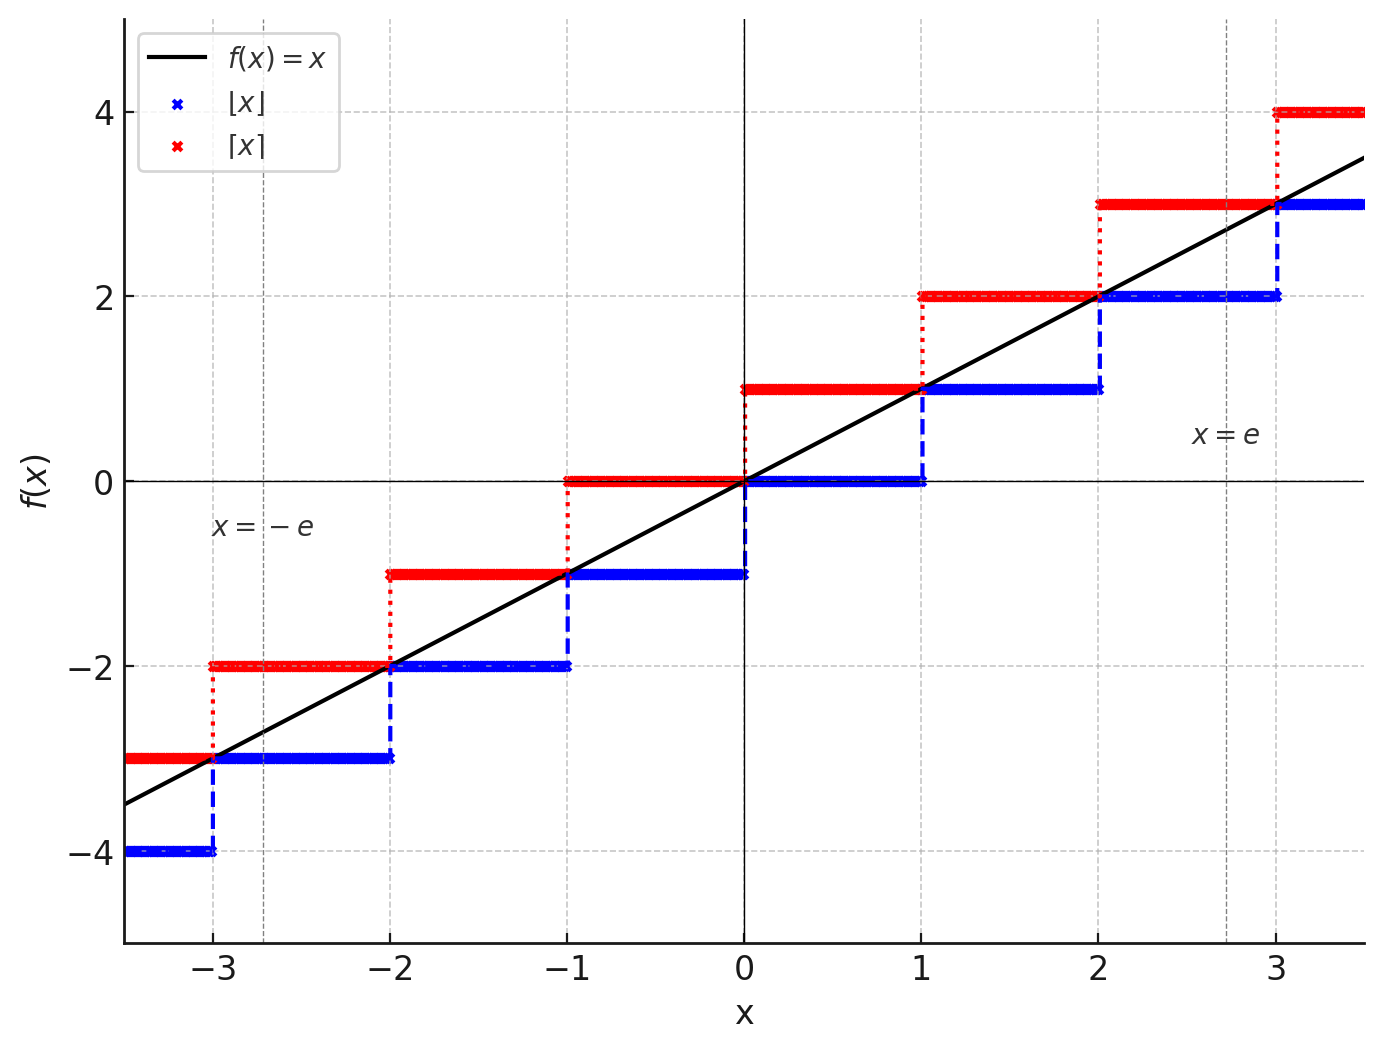
\includegraphics[width = 0.75\linewidth]{intfunc.png}
        \caption{Visualization of $\lceil x \rceil \text{ and } \lfloor x \rfloor$}
    \end{figure}

\begin{theorem}[Properties of Integer Function]
    Keep in mind the following important properties of integer function, which is 
    often used in algorithm analysis or other mathematical proof.
    \begin{enumerate}
        \item $\lfloor x \rfloor \leq x \leq \lceil x \rceil$
        \item  $\forall x\in \mathbb{Z} \text{, } \lceil x \rceil = \lfloor x \rfloor$
        \item $x \notin \mathbb{Z} \iff  \lceil x \rceil =  \lfloor x \rfloor+ 1  $
        \item $\lfloor -x \rfloor = -\lceil x \rceil $; $\lceil-x \rceil = - \lfloor x \rfloor$
        \item $x - 1 < \lfloor x \rfloor \leq x \leq \lceil x \rceil < x + 1$
    \end{enumerate}
\end{theorem}
The proofs to these conclusions are quite basic, and is therefore not provided here.

\subsubsection{Remainder and Integer Function}
We introduce a new operation that we have learned before in this section with its notation.
\begin{notation}[modulo operator]
    The modulo operation, denoted as \( a \bmod n \), finds the remainder when one integer \( a \) is divided by another integer \( n \). 
    If \( a \) divided by \( n \) gives a quotient \( q \) with remainder \( r \), then \( a = nq + r \), and \( r \) would be the result of \( a \bmod n \).
\end{notation}

Moving back to the integer function, we have:
\begin{theorem}
    $$\forall x, y \in \mathbb{R}, x \bmod y = x - y\left\lfloor \frac{x}{y} \right\rfloor, \quad \text{if } y \neq 0; \quad x \bmod 0 = x$$
\end{theorem}
Below is the proof to the first conclusion, where the properties of integer function are applied.
\begin{proof}
    By the Division Algorithm, for any integer \( x \) and any positive integer \( y \), there exist unique integers \( q \) and \( r \) such that \( x = qy + r \) and \( 0 \leq r < |y| \), where \( q \) is the quotient and \( r \) is the remainder. The floor function \( \left\lfloor \frac{x}{y} \right\rfloor \) yields the largest integer less than or equal to \( \frac{x}{y} \), which by definition is the quotient \( q \). Thus, we have:
\[
\left\lfloor \frac{x}{y} \right\rfloor = q
\]
and therefore:
\[
y\left\lfloor \frac{x}{y} \right\rfloor = yq
\]
Subtracting this from \( x \) gives:
\[
x - y\left\lfloor \frac{x}{y} \right\rfloor = x - yq = r
\]
The uniqueness of the quotient and remainder in the Division Algorithm ensures that this value of \( r \) is the remainder from the modulus operation. Therefore, we have:
\[
x \mod y = x - y\left\lfloor \frac{x}{y} \right\rfloor
\]
which is the remainder when \( x \) is divided by \( y \), completing the proof.

\end{proof}
Also, from definition, by dividing $y$ on both sides of the equation:
$$0\leq \frac{x}{y} - \lfloor\frac{x}{y}\rfloor = \frac{x \bmod y}{y} < 1$$
Among which, $x \bmod y <y$. 
\begin{proof}
    
        By the definition of the modulo operation, \( x \mod y \) can be written as \( x - y\left\lfloor \frac{x}{y} \right\rfloor \). Since \( \left\lfloor \frac{x}{y} \right\rfloor \) is the greatest integer less than or equal to \( \frac{x}{y} \), we have:
        \[
        x - y\left\lfloor \frac{x}{y} \right\rfloor \geq x - y \cdot \frac{x}{y} = x - x = 0.
        \]
        Furthermore, because \( \left \lfloor \frac{x}{y} \right\rfloor \) is less than \( \frac{x}{y} \), it follows that:
        \[
        x - y\left\lfloor \frac{x}{y} \right\rfloor < x - y \cdot \left(\frac{x}{y} - 1\right) = y.
        \]
        Hence, \( 0 \leq x \mod y < y \).

\end{proof}
And we have:
\begin{corollary}
    By above-mentioned conclusions:
    \begin{itemize}
        \item[a)] If $y > 0, \text{ then } 0 \leq x \bmod y < y$.
        \item[b)] If $y < 0, \text{ then}  0 \geq x \bmod y > y$.
        \item[c)]  $x - (x \bmod y) \text{ is an integral multiple of } y$.
    \end{itemize}
\end{corollary}
We call $x \bmod y$ the remainder when $x$ is divided by $y$. We call $\lfloor \frac{x}{y} \rfloor$ the quotient.
We have \( x \bmod y = 0 \) if and only if \( x \) is a multiple of \( y \), that is, if and only if \( x \) is divisible by \( y \). The notation \( y \mid x \), read ``\( y \) divides \( x \)'', means that \( y \) is a positive integer and \( x \bmod y = 0 \).
\subsection{exercises}
\begin{exercise}
    
        Let \( F \) be a field consisting of exactly three elements \( 0, 1, x \). Prove that \( x + x = 1 \) and that \( x \cdot x = 1 \). Obtain the addition and multiplication tables for \( F \).
        
\end{exercise}
    Hint: Think on the property of filed: inverse of addition and multiplication.
    \begin{proof}
        Since \( F \) is a field, it has the properties of both a group under addition and a group under multiplication (excluding \( 0 \) for the latter).
        
        \textbf{Part 1: Proof that \( x + x = 1 \)}
        \begin{enumerate}
            \item In a group, every element has an additive inverse. In \( F \), the additive inverse of \( 0 \) is \( 0 \) itself, since \( 0 + 0 = 0 \).
            \item The additive inverse of \( 1 \) cannot be \( 1 \) itself because \( 1 + 1 = 1 \) would imply \( 1 = 0 \), which is a contradiction. Therefore, \( 1 \)'s additive inverse must be some other element of \( F \), which can only be \( x \). Hence, \( 1 + x = 0 \).
            \item The element \( x \) must also have an additive inverse in \( F \), which cannot be \( 0 \) (as \( 0 \)'s inverse is \( 0 \)) and cannot be \( 1 \) (as \( 1 \)'s inverse is \( x \)). The only option left is \( x \) itself. Thus, \( x + x = 0 \).
            \item Given \( x + x = 0 \) and \( 1 + x = 0 \), by the cancellation law, it must be that \( x = 1 \). However, this contradicts the assumption that \( x \) is distinct from \( 1 \). Therefore, our assumption that \( x + x = 0 \) is incorrect.
            \item The only remaining possibility is \( x + x = 1 \).
        \end{enumerate}
        
        \textbf{Part 2: Proof that \( x \cdot x = 1 \)}
        \begin{enumerate}
            \item Similarly, in a multiplicative group (excluding \( 0 \)), every non-zero element has a multiplicative inverse. For \( 1 \), the multiplicative inverse is \( 1 \) itself since \( 1 \cdot 1 = 1 \).
            \item The element \( x \) must have a multiplicative inverse. It cannot be \( 0 \) since \( 0 \) is not invertible, and it cannot be \( 1 \) since \( 1 \) is already serving as its own inverse.
            \item The only remaining option for the multiplicative inverse of \( x \) is \( x \) itself. Hence, \( x \cdot x = 1 \).
        \end{enumerate}

        Now we construct the addition and multiplication tables for \( F \):

        \noindent
        \begin{minipage}{.5\textwidth}
        \centering
        \textbf{Addition Table:}
        \[
        \begin{array}{c|ccc}
        + & 0 & 1 & x \\
        \hline
        0 & 0 & 1 & x \\
        1 & 1 & x & 0 \\
        x & x & 0 & 1 \\
        \end{array}
        \]
        \end{minipage}%
        \begin{minipage}{.5\textwidth}
        \centering
        \textbf{Multiplication Table:}
        \[
        \begin{array}{c|ccc}
        \times & 0 & 1 & x \\
        \hline
        0 & 0 & 0 & 0 \\
        1 & 0 & 1 & x \\
        x & 0 & x & 1 \\
        \end{array}
        \]
        \end{minipage}
        \end{proof}
\begin{problem}
    Is there a field with exactly four elements? Is there a field with exactly six elements?
\end{problem}


\begin{exercise}
    Let \( n \) be an integer, and let \( x \) be a real number. Prove that:
\begin{enumerate}
    \item[a)] \( \lfloor x \rfloor < n \) if and only if \( x < n \);
    \item[b)] \( n \leq \lfloor x \rfloor \) if and only if \( n \leq x \);
    \item[c)] \( \lfloor x \rfloor \leq n \) if and only if \( x \leq n \);
    \item[d)] \( n < \lfloor x \rfloor \) if and only if \( n < x \);
    \item[e)] \( \lfloor x \rfloor = n \) if and only if \( x - 1 < n \leq x \) and if and only if \( n \leq x < n + 1 \);
    \item[f)] \( \lfloor x \rfloor = n \) if and only if \( x \leq n < x + 1 \) and if and only if \( n - 1 < x \leq n \).
\end{enumerate}
\end{exercise}
\begin{proof}
    \textbf{Part (a):} By definition, \( \lfloor x \rfloor \) is the greatest integer less than or equal to \( x \). Therefore, \( \lfloor x \rfloor < n \) means that \( x \) is less than \( n \) but not equal to it since \( \lfloor x \rfloor \) cannot be greater than \( x \).
    
    \textbf{Part (b):} If \( n \leq \lfloor x \rfloor \), then \( n \) must also be less than or equal to \( x \) because \( \lfloor x \rfloor \) is the greatest integer less than or equal to \( x \).
    
    \textbf{Part (c):} The statement \( \lfloor x \rfloor \leq n \) indicates that the largest integer less than or equal to \( x \) is also less than or equal to \( n \), which directly implies \( x \leq n \).
    
    \textbf{Part (d):} If \( n < \lfloor x \rfloor \), then \( n \) is strictly less than the integer part of \( x \), which means that \( n \) is also strictly less than \( x \).
    
    \textbf{Part (e):} For \( \lfloor x \rfloor = n \) to be true, \( x \) must be greater than \( n - 1 \) but not reach \( n + 1 \), hence the inequality \( x - 1 < n \leq x \) and \( n \leq x < n + 1 \).
    
    \textbf{Part (f):} Similarly, \( \lfloor x \rfloor = n \) if \( x \) has not reached \( n + 1 \) yet, which is the same as saying \( x \leq n < x + 1 \), and also if \( x \) is greater than \( n - 1 \) and less than or equal to \( n \), hence \( n - 1 < x \leq n \).
    \end{proof}

        \begin{exercise}
            Using the previous exercise, prove that \( \lfloor -x \rfloor = -\lceil x \rceil \).
            \end{exercise}
            
            \begin{proof}
                From the previous exercise, we have the following properties of the floor function for a real number \( x \) and an integer \( n \):
                \begin{enumerate}
                    \item \( x - 1 < \lfloor x \rfloor \leq x \);
                    \item \( n \leq x \) if and only if \( n \leq \lfloor x \rfloor \).
                \end{enumerate}
                Using these properties, we want to show that \( \lfloor -x \rfloor = -\lceil x \rceil \).
                
                Consider the number \( -x \). Applying property 1, we get:
                \[ -x - 1 < \lfloor -x \rfloor \leq -x \]
                Adding 1 to all parts of the inequality, we obtain:
                \[ -x < \lfloor -x \rfloor + 1 \leq -x + 1 \]
                Since \( \lceil x \rceil \) is the smallest integer greater than or equal to \( x \), \( \lfloor -x \rfloor + 1 \) is the smallest integer greater than \( -x \), which is \( -\lfloor x \rfloor \). Thus:
                \[ \lfloor -x \rfloor = -\lfloor x \rfloor - 1 = -\lceil x \rceil \]
                This completes the proof.
            \end{proof}

    \begin{exercise}
        Prove that $\displaystyle \lceil ( k-1) /2\rceil =\lfloor k/2\rfloor \ $and $\displaystyle \lfloor ( k-1) /2\rfloor =\lceil k/2\rceil \ $ $\displaystyle \forall \ k\ \in \mathbb{Z} .$
    \end{exercise}
    \begin{proof}
        We will prove the statement by cases.

        When $k$ is even, let $k=2n$. $\lceil (2n-1)/2\rceil = \lceil n - \frac{1}{2}\rceil=n, and \lfloor 2n/2\rfloor = n$.

        When $k$ is odd, let $k=2n+1$. $\lceil 2n/2 \rceil = n$, and $\lfloor2n+1/2\rfloor=\lfloor n+\frac{1}{2}=n$.
        
        The proof for $\displaystyle \lfloor ( k-1) /2\rfloor =\lceil k/2\rceil$ is similar.
    \end{proof}
%------------------------------------------------------------






\section{Algorithm and Algorithm Analysis}
	This Section discusses what is algorithm, and more importantly, how algorithms
	are assessed.

    \subsection{Algorithm}
    \subsubsection{What is an Algorithm?}
    \begin{definition}[Algorithm] \label{def:algo}
        An algorithm is a well-defined, step-by-step procedure or sequence of instructions designed to solve a specific class of problems:
        \begin{itemize}
            \item Each step in an algorithm must be clear and unambiguous. 
            \item Algorithms must be solvable, meaning they should be able to produce a correct solution for any valid input within a finite amount of time.
            \item An algorithm must terminate, i.e., it should have a defined end, at which point the goal has been achieved and the final output is produced.
        \end{itemize} 
    \end{definition}
    Here is an example of multiplication algorithm for better understanding of the concept.
    \begin{example}[Russian Peasant Multiplication]
        To find the product of integers \( M \) and \( N \), both larger than one:

        \begin{enumerate}
            \item Start two columns on a page, one labeled ``A'' and the other ``B''; and put the value of \( M \) under A and the value of \( N \) under B.
            
            \item Repeat
            \begin{itemize}
                \item[(a)] calculate a new A-value by multiplying the old A-value by 2; and
                \item[(b)] calculate a new B-value by dividing the old B-value by 2 and reducing the result by a half if necessary to obtain an integer;
            \end{itemize}
            Until the B-value equals one.
            
            \item Go down the columns crossing out the A-value whenever the B-value is even.
            
            \item Add up the remaining A-values and ``return'' the sum.
        \end{enumerate}
    \end{example}
    To show how it works, assume $A=73$ and $B=41$.

\begin{table}[H]
\centering
\begin{tabular}{c|c}
\hline
A & B \\
\hline
73 & 41 \\
146 & 20 (20\(\frac{1}{2}\) is reduced to 20) \\
292 & 10 \\
584 & 5 \\
1168 & 2 (2\(\frac{1}{2}\) is reduced to 2) \\
2336 & 1 \\
\hline
\end{tabular}
\caption{Execution of RPM}
\end{table}

Sum of the remaining A-values: $2336+584+73=2993$.

Let's review this algorithm referring to definition \autoref{def:algo}. 
\begin{enumerate}
    \item Clarity and Accuracy: All the instructions are clear and manipulable, nothing is ambiguous.
    
    \item Solvability: It is no doubt that for any two real numbers, we can find their product.
    
    \item Termination: For which ever numbers, we can always solve the problem in limited steps, as the terminate condition is when $B=1$, while B is divided by 2 (integer division) repetitively. 
\end{enumerate}

Hence, the RPM is a good example of algorithm, and with this, we could tell whether
something else is an algorithm or not.
\subsubsection{Pseudocode}
Pseudocode is a simplified, half-code, half-natural language script used by software developers and algorithm designers to outline the structure of a program or algorithm. It's not executable code, but rather a high-level representation of the algorithm's logic. The purpose of pseudo-code is to express the design of an algorithm in a form that can be easily translated into actual programming languages. It is written in a way that is understandable to people who do not necessarily know the syntax of programming languages. Pseudo-code allows the designer to focus on the core logic of the algorithm without getting bogged down with the syntactic details of a particular programming language. It often uses control structures like if-then-else, while, for, and others that are common to many high-level languages.
Understanding pseudocode is quite easy as it quite close to natural languages.

Here's the RPM transcribed in pseudocode:
\begin{algorithm}[H]
	\caption{Russian Peasant Multiplication}\label{alg:rpm}
	\begin{algorithmic}[1]
	\Procedure{RPM}{$A, B$}
		\State $product \gets 0$
		\While{$B > 0$}
			\If{$B$ is odd}
				\State $product \gets product + A$
			\EndIf
			\State $A \gets A \times 2$
			\State $B \gets B \div 2$
		\EndWhile
		\State \textbf{return} $product$
	\EndProcedure
	\end{algorithmic}
	\end{algorithm}

    To explicit:
    \begin{itemize}
        \item \textbf{procedure RPM(A, B)}: Defines a procedure or function named `RPM` taking two parameters `A` and `B`.
        \item \textbf{product $\leftarrow$ 0}: The assignment operator `$\leftarrow$` is used to assign the value on the right (0 here) to the variable on the left (`product`).
        \item \textbf{while B $>$ 0 do}: Begins a `while` loop that continues as long as the condition `B $>$ 0` is true. The `do` indicates that the following block of code will execute if the condition is met.
        \item \textbf{if B is odd then}: A conditional statement that checks if `B` is odd. If it is, the subsequent statement is executed.
        \item \textbf{product $\leftarrow$ product + A}: An assignment operation that adds `A` to `product` and assigns the sum back to `product`.
        \item \textbf{end if}: Marks the end of the `if` statement.
        \item \textbf{A $\leftarrow$ A $\times$ 2}: Multiplies the value of `A` by 2 and then assigns the result back to `A`.
        \item \textbf{B $\leftarrow$ B $\div$ 2}: Divides the value of `B` by 2 (integer division) and assigns the result back to `B`.
        \item \textbf{end while}: Marks the end of the `while` loop.
        \item \textbf{return product}: The `return` statement indicates the output or result of the procedure, which here is the value of the variable `product`.
        \item \textbf{end procedure}: Marks the end of the `RPM` procedure.
    \end{itemize}
	All later algorithms in this book will be presented using pseudocode.
%------------------------------------------------

\subsection{Algorithm Analysis}

\par Now let's take a look at this algorithm from another aspects. Is this a good or a bad algorithm. People assess algorithms by examine its \textbf{complexity}, which could be either \textbf{space complexity} or \textbf{time complexity}. The former refers to the the relationship between the input and the space needed to execute the algorithm, the latter, similarly, refers to the time needed. Many tools are available to quantify complexity, for both space and time complexity, \textbf{the big O notation} is the most common measurement. 
\begin{definition}[The Big O Notation]\label{Big O}
    Big O notation is used to classify algorithms according to how their running time or space requirements grow as the input size grows. The notation describes an upper limit on the time an algorithm could possibly take to complete, given the size of the input. For a function \( f(n) \), where n is the scale of input for the algorithm, the Big O notation is formally defined as follows with $c$ as a positive constant:
    $$O(f(n)) = \{ g(n) : \text{Where } c \text{ and } n_0 
	\text{ such that } 0 \leq g(n) \leq c \cdot f(n) \text{ for all } n \geq n_0 \}$$
\end{definition}

The following table provides common time complexities using Big O notation:

\begin{table}[ht]
\centering
\begin{tabular}{@{}cc@{}}
\toprule
\( f(n) \) & Description \\ \midrule
1 & Constant \\
\( \log n \) & Logarithmic \\
n & Linear \\
\( n \log n \) & Linearithmic \\
\( n^2 \) & Quadratic \\
\( n^3 \) & Cubic \\
\( 2^n \) & Exponential \\ 
\(n!\) & Factorial \\
\bottomrule
\end{tabular}
\caption{Common time complexities in Big O notation}
\end{table}
We can visualize it using function graph
\begin{figure}[H]
    \centering
    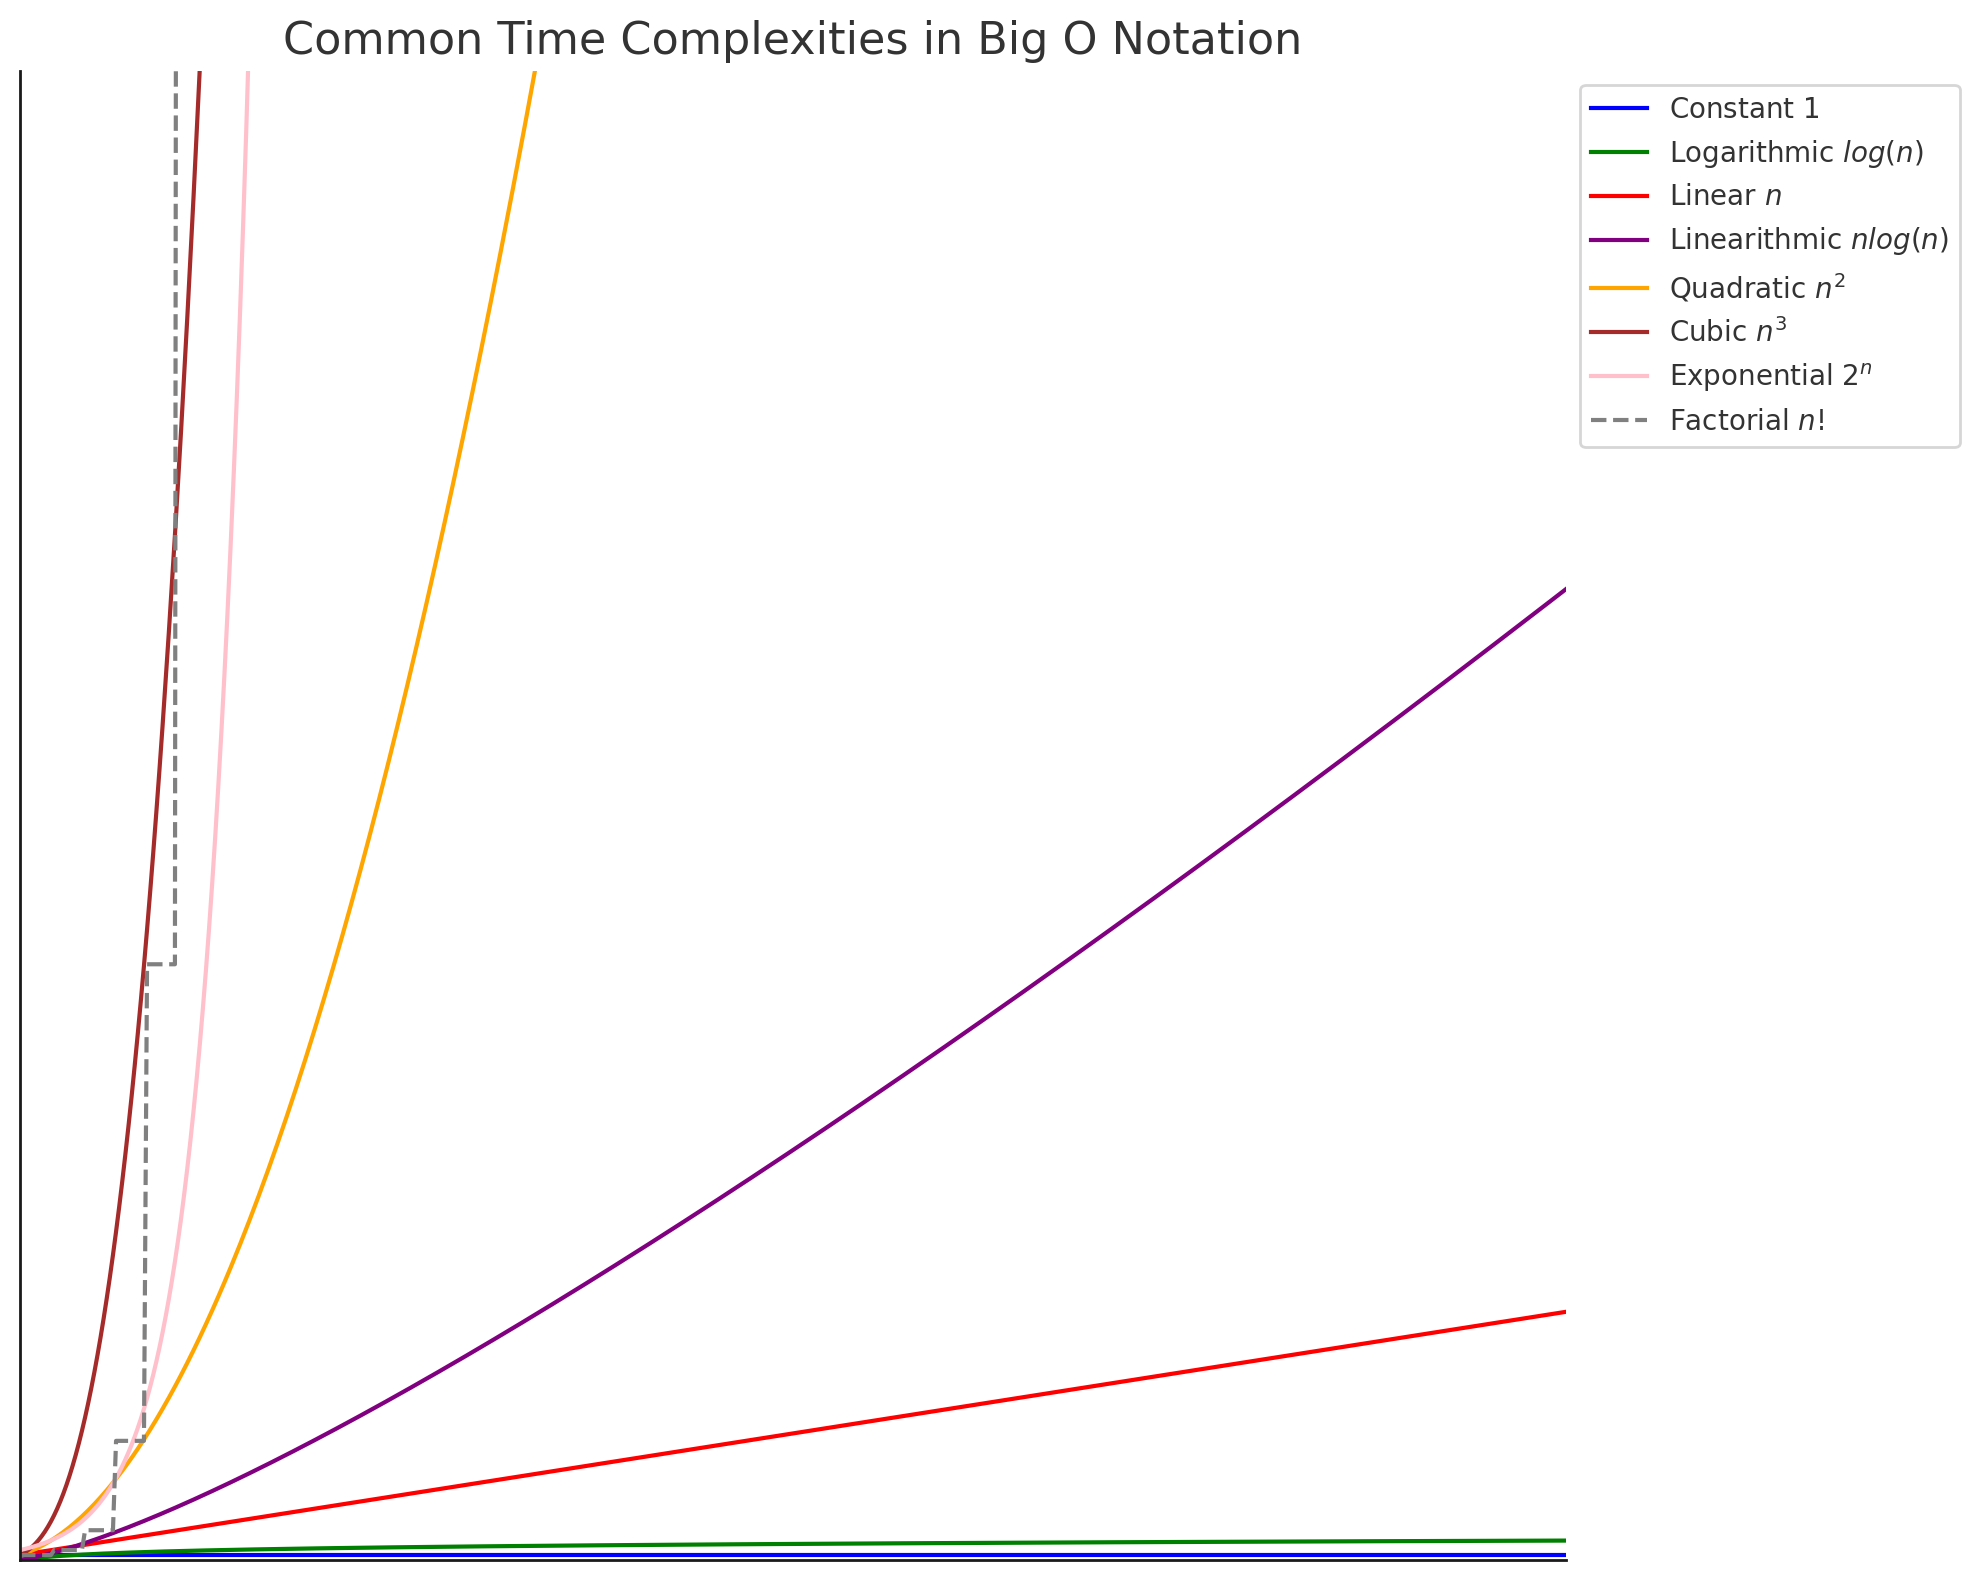
\includegraphics[width=0.8\linewidth]{Images/time complexity.png}
    \caption{Time Complexity Visualization}
    
\end{figure}
So which space and time complexity does this algorithm fall in? 
\subsubsection{Time Complexity}
To analyze the time complexity, we usually focus on the termination condition or the number of iteration for the algorithm. For the real number $B$ in RPM, each time it is divided by 2 until $B = 1$. Therefore, the total number of iteration will be $\log_2 B$, which is categorized in \( O(\log n) \).
\begin{remark}
    Actually, the time complexity of an algorithm could be shown by strict proof using MI. Here is the proof on the time complexity of RPM.
    \begin{proof}
        We will use mathematical induction to prove that the number of steps in the algorithm is proportional to \( \log_2(B) \).

\noindent \textbf{Base Case:}\\
When \( B = 1 \), the algorithm requires only one step. This is consistent with \( \log_2(1) = 0 \), which satisfies our complexity class \( O(\log n) \).

\noindent \textbf{Inductive Hypothesis:}\\
Assume that for a positive integer \( k \), when \( B = k \), the algorithm operates within \( \log_2(k) \) steps.

\noindent \textbf{Inductive Step:}\\
Consider \( B = 2k \). In the first step of the algorithm, \( B \) is halved to \( k \), and \( S \) is doubled. From this point, based on our inductive hypothesis, reaching \( B = 1 \) requires \( \log_2(k) \) steps.

Hence, for \( A = 2k \), the total number of steps is \( \log_2(k) + 1 \). Using the properties of logarithms, we have:
\begin{align*}
\log_2(k) + 1 &= \log_2(k) + \log_2(2) \\
&= \log_2(2k)
\end{align*}

Therefore, for any \( A = 2k \), the total number of steps is also \( \log_2(2k) \), proving that for any positive integer \( A \), the time complexity of the Russian Peasant Multiplication is \( O(\log A) \).
    \end{proof}
\end{remark}
%------------------------------------------------
\subsubsection{Space Complexity}
The space complexity of the Russian Peasant Multiplication algorithm is determined by the amount of memory required to store the operands and the intermediate results. Initially, only two numbers need to be stored: the multiplicands. As the algorithm proceeds, we need additional space to keep track of the current product. Since the algorithm does not use any complex data structures and only requires a fixed number of variables, the space complexity is \( O(1) \), indicating constant space usage. It does not depend on the size of the input operands, as the memory required does not increase with larger numbers.
%------------------------------------------------
\subsection{Exercises}
\begin{exercise}
    A non-recursive Square and Multiply Algorithm to calculate \( b^n \).

\textbf{Precondition:} \( n \) is a positive integer and \( b \) is of any type that can be multiplied.

\textbf{Postcondition:} the value returned is equal \( (b)^n \).

\begin{enumerate}
    \item Show that the algorithm terminates. Let \( a_k \) denote the value of \( a \) after the \( k \)th iteration of the while-loop, and let \( s = \lfloor \lg(n) \rfloor \). Prove by Mathematical Induction on \( k \) that For any nonnegative integer \( k \), after \( k \) iterations of the while-loop:
    $$2^{s-k} \le a_k < 2^{s-k+1}$$
    \item  Proof of correctness. Use Mathematical Induction on \( k \) to prove For any nonnegative integer \( k \), after \( k \) iterations of the while-loop:
\[ (\text{square})^a \times \text{product} = (b)^n \]
\end{enumerate}
\end{exercise}
\begin{algorithm}
    \caption{Square and Multiply Algorithm}
    \begin{algorithmic}[1]
    \State $product \gets 1$
    \State $square \gets b$
    \State $a \gets n$
    \While{$a > 1$}
        \If{$a \mod 2 \neq 0$} \Comment{If $a$ is odd}
            \State $product \gets product \times square$
        \EndIf
        \State $square \gets square \times square$
        \State $a \gets \lfloor a / 2 \rfloor$ \Comment{Integer division}
    \EndWhile
    \State \Return $product \times square$
    \end{algorithmic}
\end{algorithm}
\begin{proof}[1]
    \textit{Base Case} \(k=0\):
For \(k = 0\), \(a_0 = n\), which is the initial value of \(a\). Since \(s = \left\lfloor \lg(n) \right\rfloor\), it is the greatest integer less than or equal to \(\lg(n)\), therefore \(2^s \leq n < 2^{s+1}\). So, for \(k = 0\), the predicate holds because:
\[
\frac{2^s}{2^0} \leq a_0 = n < 2 \times \frac{2^s}{2^0}
\]

\textit{Inductive Step}:
Assume \(P(k)\) holds for some nonnegative integer \(k\). That is:
\[
\frac{2^s}{2^k} \leq a_k < 2 \times \frac{2^s}{2^k}
\]
We need to show \(P(k+1)\) holds. During each iteration, \(a\) is halved (integer division by 2), which gives us:
\[
a_{k+1} = \left\lfloor \frac{a_k}{2} \right\rfloor
\]

Since \(a_k\) is an integer, \(\left\lfloor \frac{a_k}{2} \right\rfloor\) will either be \(\frac{a_k}{2}\) or \(\frac{a_k - 1}{2}\), depending on whether \(a_k\) is even or odd. Thus, we have:
\[
\frac{2^s}{2^{k+1}} \leq \left\lfloor \frac{a_k}{2} \right\rfloor < 2 \times \frac{2^s}{2^{k+1}}
\]

Since \(a_k < 2 \times \frac{2^s}{2^k}\), dividing by 2 gives \(\frac{a_k}{2} < \frac{2^s}{2^k}\), and therefore:
\[
a_{k+1} < 2 \times \frac{2^s}{2^{k+1}}
\]

Similarly, \(\frac{2^s}{2^k} \leq a_k\) implies \(\frac{2^s}{2^{k+1}} \leq \frac{a_k}{2}\), so we have:
\[
\frac{2^s}{2^{k+1}} \leq a_{k+1}
\]
This completes the inductive step and thus, by induction, \(P(k)\) holds for all nonnegative integers \(k\).
\end{proof}
\begin{proof}[2]
    We need to prove that after \(k\) iterations of the while-loop, the invariant holds:
\[
(\text{square})^a \times \text{product} = b^n
\]

\textit{Base Case} \(k=0\):
Initially, \(\text{product} = 1\), \(\text{square} = b\), and \(a = n\). So,
\[
(\text{square})^a \times \text{product} = b^n
\]
is trivially true.

\textit{Inductive Step}:
Assume the invariant holds after \(k\) iterations, i.e.,
\[
(\text{square}_k)^{a_k} \times \text{product}_k = b^n
\]
Now, consider the \(k+1\)th iteration. There are two cases:

\textit{Case 1} (\(a_k\) is odd):
The product is updated by multiplying it with \(\text{square}_k\), and we have:
\[
\text{product}_{k+1} = \text{product}_k \times \text{square}_k
\]
Since \(a_k\) is odd, we can write \(a_k = 2m + 1\) for some integer \(m\), and after the iteration, \(a\) becomes \(a_{k+1} = m\). The invariant becomes:
\[
(\text{square}_k)^{2m+1} \times \text{product}_k = (\text{square}_k)^m \times \text{product}_{k+1} = b^n
\]

\textit{Case 2} (\(a_k\) is even):
The product remains the same, and \(a_k\) can be written as \(2m\), so the invariant remains:
\[
(\text{square}_k)^{2m} \times \text{product}_k = (\text{square}_k)^m \times \text{product}_k = b^n
\]
since \(\text{square}_{k+1} = (\text{square}_k)^2\) and \(a_{k+1} = m\).

In both cases, after the iteration, \(\text{square}\) is squared, so we get:
\[
\text{square}_{k+1} = (\text{square}_k)^2
\]
and therefore, the invariant still holds as:
\[
(\text{square}_{k+1})^{a_{k+1}} \times \text{product}_{k+1} = b^n
\]

Thus, by mathematical induction, the invariant holds true for every iteration of the loop, proving the correctness of the algorithm.
\end{proof}




\section{Recursion}
\subsection{Recursively Defined Algorithms and Structures}
\subsection{Structural Induction}
\chapterimage{orange2.jpg}
\chapterspaceabove{6.75cm} 
\chapterspacebelow{7.25cm} 
\chapter{Inequality}
throughout our mathematical journey, equalities are always the very basics of most conclusion, and that is also which we start to learn math for. However, inequalities are not such a know thing as equalities.
Inequalities have many tricky characteristics so that we have to take with care, or things could go wrong. This chapter covers the fundamentals of inequality as a crucial tool for problem-solving in Computer Science.

\section{Inequality basics}
We all know about inequalities, and the first thing to clarify is the relationship between sizes. How to determine the size relationship between certain numbers? Since the basis for comparing "numbers" with each other corresponds to one, it is stipulated on the number line that the points increase from left to right, and therefore the numbers they represent increase in turn. Listed in ascending order, that is:

Let \( a, b \) be two real numbers, and the points on the number line are denoted as \( A, B \) respectively. If \( A \) is to the right of \( B \), we say \( a > b \); if \( A \) is to the left of \( B \), we say \( a < b \); if \( A \) coincides with \( B \), we say \( a = b \).

Thus, for any two real numbers, one and only one of the following three situations must hold:

\[
a > b; \quad a = b; \quad a < b.
\]

The above relationship is also known as the one-dimensional coordinate law.

\[
\begin{aligned}
a > b &\Leftrightarrow a - b > 0 \\
a < b &\Leftrightarrow a - b < 0 \\
a = b &\Leftrightarrow a - b = 0
\end{aligned}
\]

Where the symbol “\( \Leftrightarrow \)” (double arrow), read as "if and only if," means that the truth of two propositions depends on each other. That is to say, if one proposition is true, then the other proposition is also true; conversely, if one proposition is false, then the other proposition is also false.

Based on the derivation of inequalities, in most cases, the above principles are sufficient. The following mathematical laws involve the geometric and algebraic meanings of the sizes of real numbers and the relationship between them. They are the basis for comparing the sizes of two real numbers and for proving inequalities by comparison. Let's review some basic properties of inequalities that are the foundation for our further study.

\begin{itemize}
    \item Symmetry: \( a > b \) if and only if \( b < a \).
    \item Transitivity: If \( a > b \) and \( b > c \), then \( a > c \).
    \item Addition (Subtraction): If \( a > b \), then \( a + c > b + c \).
    \item Multiplication (Division): If \( a > b \) and \( c > 0 \), then \( ac > bc \); if \( a > b \) and \( c < 0 \), then \( ac < bc \).
    \item Exponentiation: If \( a > b \), then \( a^n > b^n \), where \( n \) is a positive integer, and \( n \geq 2 \).
    \item Root Extraction (Power Root): If \( a > b > 0 \), then \( \sqrt[n]{a} > \sqrt[n]{b} \), where \( n \) is a positive integer, and \( n \geq 2 \).
    \item If \( a > b \) and \( c > d \), then \( a + c > b + d \).
    \item If \( a > b > 0 \) and \( c > d > 0 \), then \( ac > bd \).
\end{itemize}
\subsection{Exercises}
\begin{exercise}
    Explain the following statement.
    \begin{enumerate}
        \item If \( a > b \), then \( \frac{a}{c} > \frac{b}{c} \);
        \item If \( ac < bc \), then \( a < b \);
        \item If \( a < b \), then \( \frac{1}{a} > \frac{1}{b} \);
        \item If \( ac^2 > bc^2 \), then \( a > b \);
        \item If \( a > b \), then \( a^n > b^n \).
    \end{enumerate}
\end{exercise}

\textbf{Solution:}

\begin{enumerate}
    \item If \( c > 0 \), multiplying both sides of \( a > b \) by the positive number \( \frac{1}{c} \) preserves the inequality, hence \( \frac{a}{c} > \frac{b}{c} \). If \( c < 0 \), the direction of the inequality would be reversed, which is not given in the condition, hence we assume \( c > 0 \).
    \item Dividing both sides of \( ac < bc \) by \( c \) (assuming \( c \neq 0 \)), we get \( a < b \) because division by a positive number preserves the inequality, and division by a negative number reverses it.
    \item Taking the reciprocal of both sides of \( a < b \) reverses the inequality because \( a \) and \( b \) are on opposite sides of the fraction line, hence \( \frac{1}{a} > \frac{1}{b} \) (assuming \( a, b > 0 \) to avoid division by zero).
    \item Dividing both sides of \( ac^2 > bc^2 \) by \( c^2 \) (assuming \( c \neq 0 \)) preserves the inequality, hence \( a > b \) because \( c^2 \) is positive regardless of whether \( c \) is positive or negative.
    \item Raising both sides of \( a > b \) to a power \( n \) (assuming \( n \) is a positive integer) preserves the inequality because both \( a \) and \( b \) are raised to the same power, hence \( a^n > b^n \).
\end{enumerate}
\begin{exercise}
    Given the inequality \( a > b > 0 \), \( c < d < 0 \), \( f < 0 \), show that:
\[
\frac{f}{a - c} > \frac{f}{b - d}.
\]
\end{exercise}
\begin{proof}
    Since \( a > b > 0 \) and \( c < d < 0 \), then \( a - c > b - d \) because subtracting a smaller negative number is the same as adding a larger positive number. Given that \( f < 0 \), when dividing by a larger positive number, the result is smaller because a negative number divided by a positive number yields a negative result, and the further away the divisor is from zero, the smaller the quotient.

Therefore:
\[
\frac{f}{a - c} > \frac{f}{b - d}.
\]
\end{proof}

\section{Solving Quadratic Inequality}
Recall that, when we solve Quadratic equations, we use discriminant to solve equations, which is also applicable to inequalities.
For a quadratic inequality of the form $ax^2 + bx + c > 0$ or $ax^2 + bx + c < 0$ (where $a > 0$), the solution set can be determined by the discriminant $\Delta = b^2 - 4ac$:
\begin{enumerate}
    \item If $\Delta > 0$, the quadratic equation $ax^2 + bx + c = 0$ has two distinct real roots $x_1$ and $x_2$, and $x_1 < x_2$. The solution set for $y = ax^2 + bx + c$ being greater than zero (when $y = 0$) is for values of $x$ either less than $x_1$ or greater than $x_2$, and the solution set for $ax^2 + bx + c < 0$ is $\{ x \mid x_1 < x < x_2 \}$.
    \item If $\Delta = 0$, then $ax^2 + bx + c = 0$ has one real root, specifically $x_1 = x_2 = -\frac{b}{2a}$. The solution set for $y = ax^2 + bx + c$ being greater than zero is all $x$ except $x \neq -\frac{b}{2a}$, and there is no solution set where $ax^2 + bx + c < 0$.
    \item If $\Delta < 0$, then $ax^2 + bx + c = 0$ has no real roots, and the parabola $y = ax^2 + bx + c$ does not intersect the x-axis. The solution set for $ax^2 + bx + c > 0$ is all real numbers, and there is no solution set where $ax^2 + bx + c < 0$.
\end{enumerate}
\begin{figure}[ht!]
    \centering
    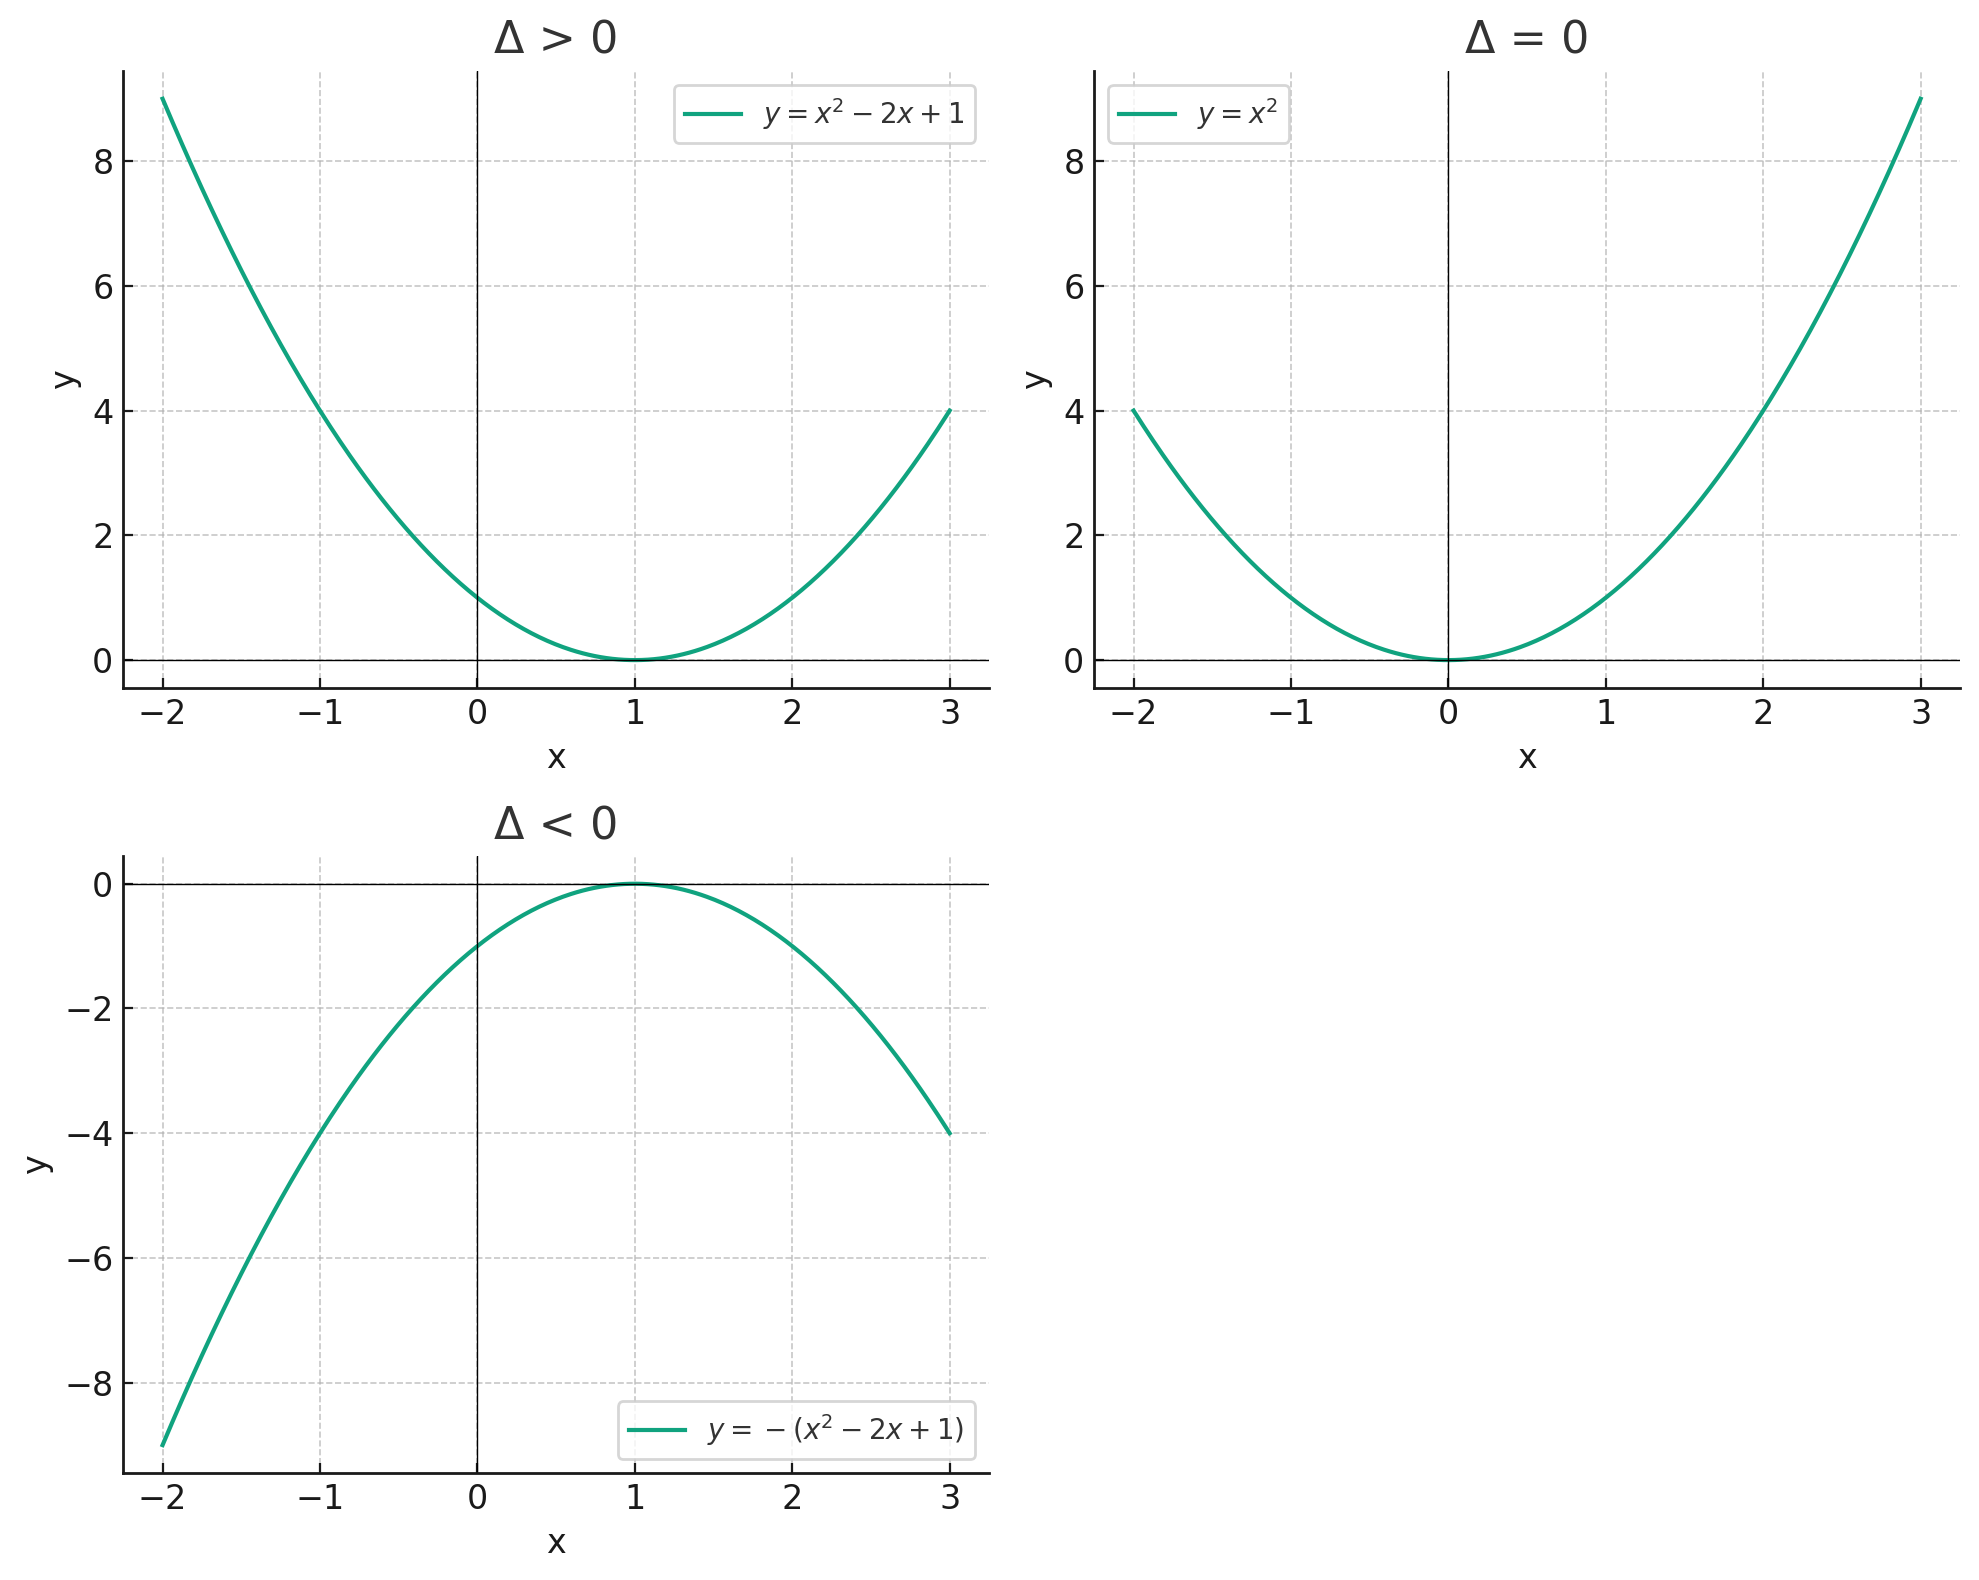
\includegraphics[width=0.8\textwidth]{quadratic.png}
    \caption{Quadratic function graphs based on the discriminant.}
\end{figure}
\begin{example}
    Solve the following quadratic inequalities:

\begin{enumerate}
    \item \(4x^2 + 6x + 2 < 0\);
    \item \(4x^2 + 4x + 1 < 0\);
    \item \(-3x^2 + x - 6 < 0\).
\end{enumerate}
\end{example}
\textbf{Solution:}

\begin{enumerate}
    \item The discriminant \(\Delta = 6^2 - 4 \times 4 \times 2 = 4 > 0\), so the quadratic equation \(4x^2 + 6x + 2 = 0\) has two real roots \(x_1 = -1\), \(x_2 = -\frac{1}{2}\).
    Hence, the solution set for the inequality is \(x \in \left(-\infty, -1\right) \cup \left(-\frac{1}{2}, \infty\right)\).

    \item The discriminant \(\Delta = 4^2 - 4 \times 4 \times 1 = 0\), so the quadratic equation \(4x^2 + 4x + 1 = 0\) has one real double root. Therefore, the inequality has no solution set.

    \item The discriminant \(\Delta = 1^2 - 4 \times (-3) \times (-6) = -71 < 0\), so the quadratic equation \(-3x^2 + x - 6 = 0\) has no real roots.
    Therefore, the solution set for the inequality \(3x^2 - x + 6 > 0\) is all real numbers, and thus the solution set for the given inequality is also all real numbers.
\end{enumerate}

\section{important Inequalities}
In this part, we explore two fundamental inequalities in mathematics: the Triangle Inequality and the Arithmetic-Geometric Mean (AGM) Inequality. Each section provides a comprehensive overview, including detailed proofs and corollaries.
\subsection{The Triangle Inequality}
The Triangle Inequality is a fundamental relation in geometry and analysis, asserting that the sum of the lengths of any two sides of a triangle must be greater than or equal to the length of the remaining side.
    \begin{definition}[Triangular Inequality] \label{triangularineq}
        For any real numbers \( a \) and \( b \), the Triangle Inequality is given by:
        \[ |a + b| \leq |a| + |b| \]
    \end{definition}
    \begin{proof}
        The proof of the Triangle Inequality considers the sign of \( a \) and \( b \):
    \begin{itemize}
     \item \textbf{Case 1:} If \( a \) and \( b \) have the same sign, the inequality follows directly.
        \item \textbf{Case 2:} If \( a \) and \( b \) have opposite signs, assume \( a > 0 \) and \( b < 0      \). Then, \( |a + b| \leq a - b = |a| + |b| \).
    \end{itemize}
    Thus, the Triangle Inequality is proven.
    \end{proof}
    \begin{remark}
        This important inequality will also be seen in other chapters.
    \end{remark}
We also have the following conclusion by preliminary algebra:
$$
\begin{aligned}
    |a{+}b|{\leqslant}|a|+|b|& \Leftrightarrow|a{+}b|^2{\leqslant}(|a|{+}|b|)^2  \\
    &\Leftrightarrow(a+b)^2\leqslant|a|^2+2|a||b|+|b|^2 \\
    &\Leftrightarrow a^2+2ab+b^2\leqslant a^2+2|a|\mid b|+b^2 \\
    &\Leftrightarrow ab{\leqslant}|a|\left|b\right| \\
    &\Leftrightarrow ab\leqslant\lvert ab\rvert.
    \end{aligned}
$$
The quality holds only when $ab \geq 0$.
\subsubsection*{Geometric Explanation of Triangular Inequality}
    Consider $a$ and $b$ are random numbers on a number axis:
    \begin{itemize}
        \item If $ab \geq 0$, then they are both in the same half-axis (both positive or negative). In this case, the distance between $a$ and $-b$
        is the sum of the distance from both points to the origin of the number axis.
        \item  Now consider $ab < 0$, either of them is positive, and the other is negative. In this case, the distance between $a$ and $-b$ is shorter than the sum of 
        the distance from both points to the origin of the number axis.
        \begin{figure}[H]
            \centering
            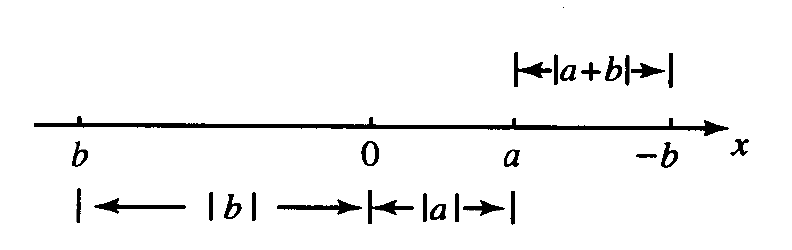
\includegraphics[width = 0.6\textwidth]{triangleablt0.png}
            \caption{Triangular Inequality: $ab < 0$}
        \end{figure}
    \end{itemize}

We also have:
    \begin{theorem}
        For $a, b, c\in \mathbb{R}$, $|a-c|\leq |a-b| + |b-c|$.
    \end{theorem}
    \begin{figure}[H]
        \centering
        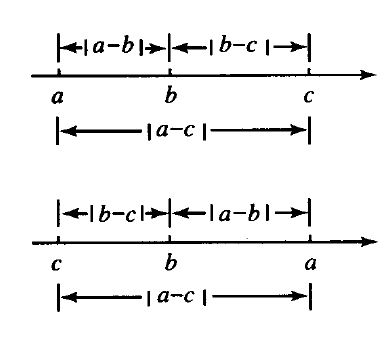
\includegraphics[width = 0.5\textwidth]{triangle2.png}
    \end{figure}
    \begin{proof}
        Since $a-c$, $a-b$, $b-c$ follows the relationship of triangular inequality. We have:
        $$(a-b)(b-c) \geq 0$$
        
        meaning that $b$ is between $a$ and $c$, which could be proven by sketching.
    \end{proof}

    \begin{corollary} \label{trian}
        $||a| - |b|| \leq |a + b|$
    \end{corollary}
    \begin{proof}
        \[ |a| = |(a+b) - b| \leq |a+b| + |-b| = |a+b| + |b|. \]
Therefore,
\[ |a| - |b| \leq |a+b|, \]
and similarly it can be proven that
\[ |b| - |a| \leq |a+b|. \]
Hence,
\[ ||a - b|| \leq |a+b|. \]
    \end{proof}

    \begin{corollary}
        $|a| - |b| \leq |a + b|$
        
    \end{corollary}
    \begin{proof}
        By corollary \autoref{trian}:
        \[ ||a| - |b|| \leq |a + (-b)|, \]
therefore,
\[ ||a| - |-b|| \leq |a - b|. \]
    \end{proof}
%---------------------------------------------------------------------------
    \subsection{The Arithmetic-Geometric Mean Inequality}
    The AGM Inequality(also known as AM-GM inequality) states that for any set of non-negative real numbers, the arithmetic mean is always greater than or equal to the geometric mean.
    \begin{definition}[AGM Inequality] \label{AGM}
        For non-negative real numbers \( a_1, a_2, \ldots, a_n \), the AGM Inequality is:
        \[ \frac{a_1 + a_2 + \cdots + a_n}{n} \geq \sqrt[n]{a_1 \cdot a_2 \cdots a_n} \]
    \end{definition}
    Many methods are available to prove this important conclusion. Below is the proof by MI.
    \begin{proof}
        We prove that for any non-negative real numbers \(x_1, \ldots, x_n\), the following inequality holds:

\[
\alpha^n \geq x_1 x_2 \cdots x_n
\]

where \( \alpha \) is the arithmetic mean of the numbers, with equality if and only if all the numbers are equal.
\begin{remark}
    This is because, the inequality is equivalent to AGM:
    $$\frac{a_{1} +a_{2} +\dotsc +a_{n}}{n} \geq \sqrt[n]{a_{1} \cdot a_{2} \dotsc a_{n}} \Longleftrightarrow \left(\frac{a_{1} +a_{2} +\dotsc +a_{n}}{n}\right)^{n} \geq a_{1} \cdot a_{2} \dotsc a_{n}$$

\end{remark}
\textbf{Induction Basis:}
For \(n = 1\), the statement is trivially true, as the arithmetic mean of a single number is the number itself.

\noindent \textbf{Induction Hypothesis:}
Assume that the AM-GM inequality holds for \(n\) non-negative real numbers.

\noindent \textbf{Induction Step:}
Consider \(n+1\) non-negative real numbers \(x_1, \ldots, x_{n+1}\). Their arithmetic mean \( \alpha \) satisfies:

\[
\alpha = \frac{x_1 + \cdots + x_n + x_{n+1}}{n+1}
\]

If all the \(x_i\) are equal to \( \alpha \), then we have equality in the AM-GM statement, and we are done. In the case where some are not equal to \( \alpha \), there must exist at least one number greater and one smaller than \( \alpha \). Without loss of generality, we can reorder our \(x_i\) to ensure that \(x_n > \alpha > x_{n+1}\), which gives us:
\begin{equation}
    (x_n - \alpha)(\alpha - x_{n+1}) > 0 \label{agm1}
\end{equation}


Define a new number \( y \) with:

\[
y = x_n + x_{n+1} - \alpha \geq x_n - \alpha > 0
\]
Since all numbers from $x_1$ to $y$  are non-negative.

$$\begin{aligned}&(n+1)\alpha=x_1+\cdots+x_{n-1}+x_n+x_{n+1}\\&n\alpha=x_1+\cdots+x_{n-1}+\underbrace{x_n+x_{n+1}-\alpha}_{=y},\end{aligned}$$

This shows that $\alpha$ is also a geometric mean of the n-sequence $x_{1},\ldots,x_{n-1},y$. 

By the induction hypothesis:
$$\alpha^{n+1}=\alpha^n\cdot\alpha\geq x_1x_2\cdots x_{n-1}y\cdot\alpha.$$

From equation \autoref{agm1}, we have:
$$(\underbrace{x_n+x_{n+1}-\alpha}_{=y})\alpha-x_nx_{n+1}=(x_n-\alpha)(\alpha-x_{n+1})>0,$$

Hence:
$$y\cdot \alpha > x_n x_{n+1}$$
By substituting we have:
$$\alpha^{n+1}>x_1x_2\cdots x_{n-1}x_nx_{n+1}$$
This completes the proof.
\end{proof}

\subsubsection*{Geometric representation}
We can use function graphs to visualize the relationship implied in the AGM inequality. On the left and right-hand-side of the inequality sign, there are two functions with $n$ variables.
For simplicity, we use $n=2$ to show its visualization.
We obtain this interactive graph by Mathematica. This simple model involves three variables only. $\displaystyle x_{1}$ and $\displaystyle x_{2}$ are the values to be used to calculate AM and GM. 
We take one of the input value as preimage on the x-axis, and the AM or GM as the image on y-axis. The scroll on the top indicates the value of $\displaystyle x_{2}$. When $\displaystyle x_{2} =0$, the 
graph is shown below. It can be seen that the AGM inequality holds, and only when $\displaystyle x_{2} =x_{1} =0$, there is an intersection$\displaystyle \ ( 0,0) .$

\begin{figure}[H]
    \centering
    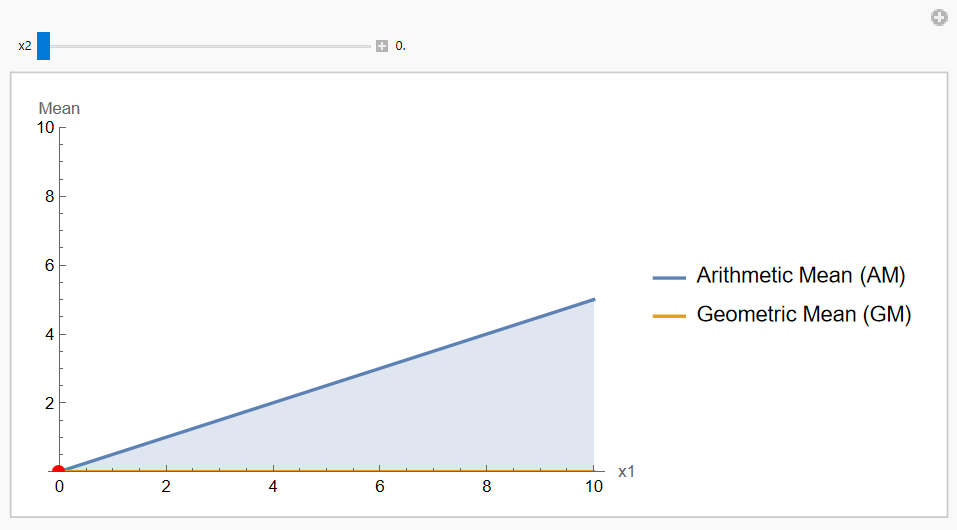
\includegraphics[width=0.8\textwidth]{agmx=0.png}
    \caption{AGM when $x_2 = 0$}
\end{figure}

As we increase the $\displaystyle x_{2}$ value, the GM curve rise up, and the intersection moves on the right direction, remaining on the AM curve. Below is the visualization for $\displaystyle x_{2} =5$. 
There is no any overlap between graphs except the intersection $\displaystyle ( 5,5)$. 

\begin{figure}[H]
    \centering
    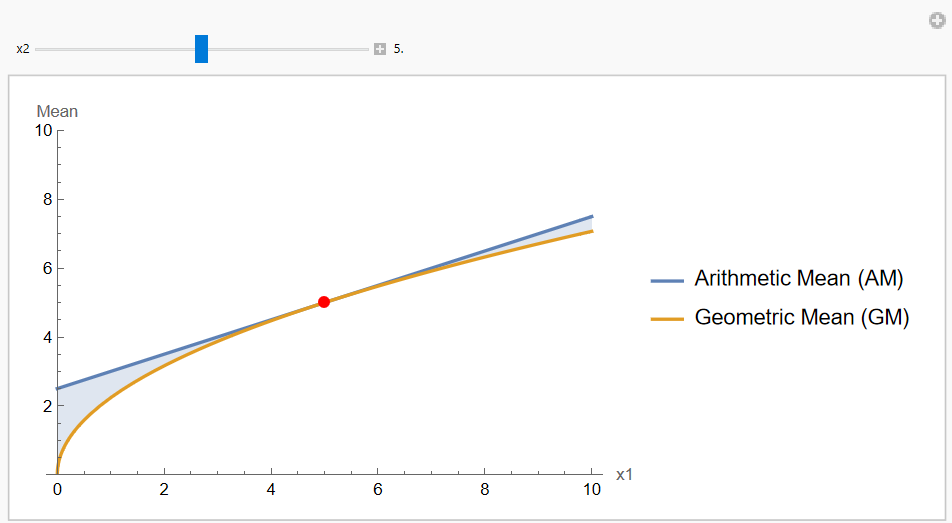
\includegraphics[width=0.8\textwidth]{agmx=5.png}
    \caption{AGM when $x_2 = 5$}
\end{figure}

\begin{problem}
    Where will the intersection go if we have $x_2 = 10$ for this model?
\end{problem}

Now, I think everything is clear, but only things so far. From now on, we will extend the understanding of function graph to a new
dimension, in the 3 dimension space. Functions in the 3D space is extremely important for multi-variable calculus, and learning linear 
algebra also requires us to abstract numbers in more than 3 dimension, but goes up to n dimension space. But don't worry, the discussion
here only involve simple concepts. 

We have three variables: $x_1, x_2, y$, where $y$ is the value of AM or GM from $x_1$ and $x_2$. Coincidently, we have three coordinate
axis in a 3D space. In the three-dimensional coordinate system, we assign two preimages $x_1$, $x_2$ to $x$ and $y$ axis, and the mean
to the $z$ axis. In this way we can get two function graphs, or surface, in the real sense, in the coordinate, which look like in the 
figure below.
\begin{figure}[H]
    \centering
    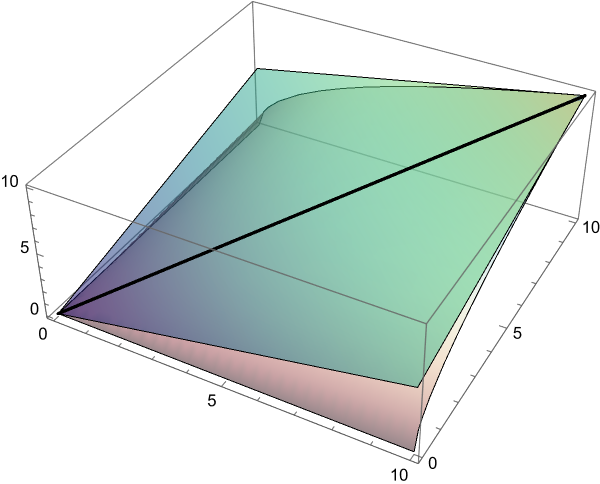
\includegraphics[width=0.6\textwidth]{agm3D.png}
    \caption{AGM 3D Visualization}
\end{figure}

The plane in blue represents the set of all possible arithmetic mean derived from all combinations of $x_1 \text{ and }x_2$ with $x_1,x_2\in [0,10]$, and the other 
surface, almost below the AM plane, is exactly the geometric mean curve that has a similar definition to the former. This is quite different from the functions
we have known, since they are only a line or a curve in the Cartesian coordinate, yet in the 3D coordinate, function could be surface. We will explore more
about multi-variable functions in the future. 

It is noticeable that the two surfaces are actually independent. They intersect in a line that go across the space. That specific line is actually a set of all the
ordered pairs $(x_1,x_2)$ where $x_1 = x_2$. We can actually relate it to the graph in the Cartesian coordinate. If we change the view point to the front of the
curves shaped in the 3D space, we see something like this picture.
\begin{figure}[H]
    \centering
    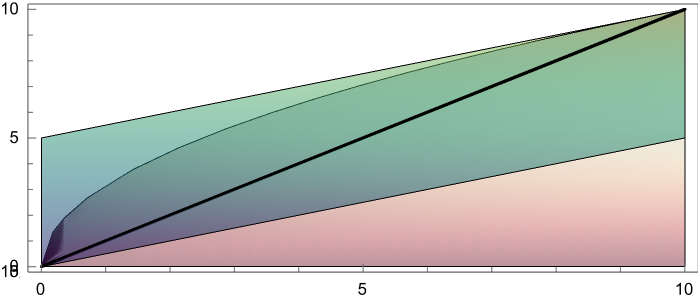
\includegraphics[width=0.6\textwidth]{agm3dsect.png}
    \caption{AGM 3D Visualization (Front)}
\end{figure}
Isn't this quite similar to the 2D graph? Actually, the first image is exactly a horizontal cross-section of the 3D function graph, and the intersection in the 2D 
graph changes as the position of intersection line changes. These explain AGM inequality's geometric meaning.

\subsection*{Conclusions of AGM inequality}
AGM inequality has brought us to these conclusions:
    \begin{corollary}[Mean Inequality Corollary]
If $x, y > 0$, then
\[\frac{2xy}{x+y} \leq \sqrt{xy} \leq \frac{x+y}{2}.\]
Equality holds in each inequality only when $x = y$.
\end{corollary}

\begin{proof}
Proposition \ref{AGM} yields $\sqrt{xy} \leq \frac{x+y}{2}$. We obtain the other inequality from this by multiplying both sides by the positive number $\frac{2\sqrt{xy}}{x+y}$, leading to:
\[\sqrt{xy} \cdot \frac{2\sqrt{xy}}{x+y} \leq \frac{x+y}{2} \cdot \frac{2\sqrt{xy}}{x+y},\]
which simplifies to:
\[\frac{2xy}{x+y} \leq \sqrt{xy}.\]
Thus, we have shown that $\frac{2xy}{x+y} \leq \sqrt{xy} \leq \frac{x+y}{2}$, with equality if and only if $x = y$.
\end{proof}
The expression $\frac{2xy}{x+y}$ is the harmonic mean of $x$ and $y$. It arises in the study of average rates. For example, consider traveling a distance $d$ at rate $r_1$ in time $t_1$ and making the return trip at rate $r_2$ in time $t_2$. The harmonic mean gives us the average rate $r$ for the full trip.

Assuming we travel the same distance $d$ for both trips, we have:
\begin{align*}
r_1t_1 &= d \\
r_2t_2 &= d
\end{align*}

The average rate $r$ for the full trip is computed as follows:
\begin{align*}
r &= \frac{2d}{t_1 + t_2} = \frac{2d}{\frac{d}{r_1} + \frac{d}{r_2}} = \frac{2d}{\frac{r_1r_2(t_1 + t_2)}{r_1r_2}} =\frac{2r_1r_2}{r_1 + r_2}\\
\end{align*}

The other important corollary of AGM inequality is:
\begin{corollary}
    $a^2+b^2 \geq 2ab$
\end{corollary}
\begin{proof}
    $a^2 + b^2 \geq 2ab \iff a^2 + b^2 - 2ab \geq 0 \iff (a - b)^2 \geq 0.$
\end{proof}


\subsection{Exercises}
\begin{exercise}
    Prove that for any triangle with sides \(a\), \(b\), and \(c\), the following inequality holds:
\[ \frac{a}{b + c} + \frac{b}{a + c} + \frac{c}{a + b} > 1 \]
\end{exercise}
\begin{proof}

Given a triangle with sides \(a\), \(b\), and \(c\), we know that for any triangle, the sum of the lengths of any two sides is greater than the length of the third side. Therefore, \(a < b + c\), \(b < a + c\), and \(c < a + b\).

Now, consider the inequality \(\frac{a}{b + c} > \frac{a}{a + b + c}\). This is true because \(b + c > a\) implies that the denominator of the left-hand side is smaller than that of the right-hand side while keeping the numerator constant.

Similarly, we can show that \(\frac{b}{a + c} > \frac{b}{a + b + c}\) and \(\frac{c}{a + b} > \frac{c}{a + b + c}\).

Adding these three inequalities, we get:
\[ \frac{a}{b + c} + \frac{b}{a + c} + \frac{c}{a + b} > \frac{a + b + c}{a + b + c} \]

Simplifying the right-hand side, we obtain:
\[ \frac{a}{b + c} + \frac{b}{a + c} + \frac{c}{a + b} > 1 \]

Thus, the inequality is proven. 

\end{proof}

\begin{exercise}
    Given $\varepsilon > 0$, if $|x - a| < \frac{\varepsilon}{4}$ and $|y - b| < \frac{\varepsilon}{6}$, prove that:

\[
|2x + 3y - 2a - 3b| < \varepsilon.
\]
\end{exercise}
Hint: Rearrange it in a form that is good for using triangle inequality.
\begin{proof}
    \begin{align*}
        |2x + 3y - 2a - 3b| &= |2(x - a) + 3(y - b)| \\
        &\leq |2(x - a)| + |3(y - b)| \\
        &= 2|x - a| + 3|y - b| \\
        &< 2 \times \frac{\varepsilon}{4} + 3 \times \frac{\varepsilon}{6} \\
        &= \varepsilon.
        \end{align*}
\end{proof}

\begin{exercise}
    Prove for any real numbers \( a, b, c, d \) that:
\[ |a - b| + |b - c| + |c - d| + |d - a| \geq |a - c| + |b - d| \]

\end{exercise}

\begin{proof}
    \begin{enumerate}
    \item \textbf{Application of the Triangle Inequality:}
    The triangle inequality states that for any real numbers \( x, y, z \):
    \[ |x - y| \leq |x - z| + |z - y| \]
    We can apply this inequality to certain terms in our original problem. For example, consider \( |a - c| \) and \( |b - d| \).

    \item \textbf{Separate Applications of the Triangle Inequality:}
    For \( |a - c| \), we have:
    \[ |a - c| \leq |a - b| + |b - c| \]
    For \( |b - d| \), we have:
    \[ |b - d| \leq |b - c| + |c - d| \]

    \item \textbf{Combining Inequalities:}
    Adding the above two inequalities, we get:
    \[ |a - c| + |b - d| \leq |a - b| + 2|b - c| + |c - d| \]

    \item \textbf{Simplification and Rearrangement:}
    Notice that \( 2|b - c| \) appears on the right side of the inequality. However, since \( |b - c| \) is non-negative, we can remove one \( |b - c| \) and the inequality still holds. Hence, we have:
    \[ |a - c| + |b - d| \leq |a - b| + |b - c| + |c - d| \]
    This is the reverse of the inequality in our original problem, so we can conclude:
    \[ |a - b| + |b - c| + |c - d| + |d - a| \geq |a - c| + |b - d| \]

    \item \textbf{Conclusion:}
    Therefore, the original inequality is proved.
\end{enumerate}
\end{proof}
\begin{exercise}
    Prove that for any real numbers \( x, y, z \), the following inequality holds:
\[ |x + y + z| \leq |x| + |y| + |z| \]

\end{exercise}
\begin{proof}
    We will use the triangle inequality which states that for any real numbers \( a \) and \( b \):
\[ |a + b| \leq |a| + |b| \]

First, apply the triangle inequality to \( x \) and \( y \):
\[ |x + y| \leq |x| + |y| \]

Now, let \( a = x + y \) and \( b = z \), and apply the triangle inequality again:
\[ |(x + y) + z| \leq |x + y| + |z| \]

Substitute the first inequality into the second one:
\[ |x + y + z| \leq |x| + |y| + |z| \]

This completes the proof.
\end{proof}
\begin{exercise}
    Prove that for any sequence of real numbers \( x_1, x_2, \ldots, x_n \), the following inequality holds:
\[ \left|x_1 + x_2 + \ldots + x_n\right| \leq \left|x_1\right| + \left|x_2\right| + \ldots + \left|x_n\right| \]
\end{exercise}
\begin{proof}
    We will prove this by induction on the number of terms \( n \).

\textit{Base case} (\( n = 1 \)):
For a single real number \( x_1 \), the inequality trivially holds as:
\[ \left|x_1\right| = \left|x_1\right| \]

\textit{Inductive step}:
Assume the inequality holds for some \( n = k \), i.e.,
\[ \left|x_1 + x_2 + \ldots + x_k\right| \leq \left|x_1\right| + \left|x_2\right| + \ldots + \left|x_k\right| \]
Now, consider the case when \( n = k + 1 \). By the triangle inequality, we have:
\[ \left|x_1 + x_2 + \ldots + x_k + x_{k+1}\right| \leq \left|x_1 + x_2 + \ldots + x_k\right| + \left|x_{k+1}\right| \]

Using the induction hypothesis, we can then write:
\[ \left|x_1 + x_2 + \ldots + x_k + x_{k+1}\right| \leq \left(\left|x_1\right| + \left|x_2\right| + \ldots + \left|x_k\right|\right) + \left|x_{k+1}\right| \]
\[ \left|x_1 + x_2 + \ldots + x_k + x_{k+1}\right| \leq \left|x_1\right| + \left|x_2\right| + \ldots + \left|x_k\right| + \left|x_{k+1}\right| \]

This completes the inductive step and thus, by the principle of mathematical induction, the inequality holds for all positive integers \( n \).
\end{proof}

\begin{exercise}
    Let \(a\), \(b\), \(c\) be positive real numbers. Prove the inequality:
\[ (a+b+c)(a^2+b^2+c^2) > 9abc. \]
\end{exercise}
\begin{proof}
    By the Arithmetic Mean-Geometric Mean Inequality (AM-GM Inequality), we have:
\[ \frac{a^2+b^2+c^2}{3} \geq \sqrt[3]{a^2b^2c^2}, \]
\[ \frac{a+b+c}{3} \geq \sqrt[3]{abc}. \]

Cubing both sides of the inequalities, we get:
\[ (a^2+b^2+c^2)^3 \geq 27a^2b^2c^2, \]
\[ (a+b+c)^3 \geq 27abc. \]

Multiplying the resulting inequalities, we obtain:
\[ (a^2+b^2+c^2)^3(a+b+c)^3 \geq (27a^2b^2c^2)(27abc). \]

Taking the cube root of both sides, we arrive at:
\[ (a^2+b^2+c^2)(a+b+c) \geq 9abc. \]

Note that the inequality is strict when \(a\), \(b\), \(c\) are positive real numbers, thus:
\[ (a^2+b^2+c^2)(a+b+c) > 9abc. \]
\end{proof}

\begin{exercise}
    Given non-negative real numbers \( a, b, c \) such that \( a + b + c = 1 \), we want to prove that:
\[ a^2 + b^2 + c^2 \geq \frac{1}{3}. \]
\end{exercise}
\begin{proof}
    We will use the Arithmetic Mean-Geometric Mean Inequality (AM-GM Inequality) which states that for any non-negative real numbers \( x, y, z \), the following holds:
\[ \frac{x + y + z}{3} \geq \sqrt[3]{xyz}. \]

Applying this to \( a, b, c \), we have:
\[ \frac{a + b + c}{3} \geq \sqrt[3]{abc} \Rightarrow \frac{1}{3} \geq \sqrt[3]{abc}. \]

Cubing both sides of the inequality yields:
\[ \frac{1}{27} \geq abc. \]

Now, by AM-GM applied to \( a^2, b^2, c^2 \), we get:
\[ \frac{a^2 + b^2 + c^2}{3} \geq \sqrt[3]{a^2b^2c^2}. \]

Since \( a^2b^2c^2 \) is the square of \( abc \), it follows that:
\[ \frac{a^2 + b^2 + c^2}{3} \geq (abc)^{\frac{2}{3}}. \]

Given \( \frac{1}{27} \geq abc \), we have:
\[ (abc)^{\frac{2}{3}} \leq \left(\frac{1}{27}\right)^{\frac{2}{3}} = \frac{1}{9}. \]

Therefore, we can conclude that:
\[ \frac{a^2 + b^2 + c^2}{3} \geq \frac{1}{9}. \]

Multiplying through by 3, we obtain the desired inequality:
\[ a^2 + b^2 + c^2 \geq \frac{1}{3}. \]

Hence, we have proved that \( a^2 + b^2 + c^2 \geq \frac{1}{3} \) as required.
\end{proof}

\begin{exercise}
    Consider the function
    \[
    f(x, y, z) = \frac{x}{y} + \frac{y}{z} + \frac{z}{x}
    \]
    for all positive real numbers \( x, y, \) and \( z \). Find the minimal value of the function.
    \end{exercise}
    
    \begin{proof}
    For \( (x, y, z) \) positive real numbers, we have
    \[
    f(x, y, z) = \frac{x}{y} + \frac{y}{z} + \frac{z}{x}
    \]
    can be rewritten as
    \[
    f(x, y, z) = 6 \cdot \left( \frac{1}{6} \cdot \frac{x}{y} + \frac{1}{6} \cdot \frac{y}{z} + \frac{1}{6} \cdot \frac{z}{x} + \frac{1}{6} \cdot \frac{x}{y} + \frac{1}{6} \cdot \frac{y}{z} + \frac{1}{6} \cdot \frac{z}{x} \right)
    \]
    Setting \( x_1 = \frac{x}{y}, x_2 = x_3 = \frac{1}{2} \cdot \frac{y}{z}, x_4 = x_5 = x_6 = \frac{1}{3} \cdot \frac{z}{x} \), and applying the AM-GM inequality for \( n = 6 \), we get
    \[
    f(x, y, z) \geq 6 \cdot \sqrt[6]{x_1 \cdot x_2 \cdot x_3 \cdot x_4 \cdot x_5 \cdot x_6} = 6 \cdot \sqrt[6]{\frac{1}{2 \cdot 2 \cdot 3 \cdot 3 \cdot 3} \cdot \frac{x}{y} \cdot \frac{y}{z} \cdot \frac{z}{x}}
    \]
    which simplifies to
    \[
    f(x, y, z) \geq 6 \cdot \sqrt[6]{\frac{1}{2^2 \cdot 3^3}} = 2^{2/3} \cdot 3^{1/2}
    \]
    Further, we know that the two sides are equal exactly when all the terms of the mean are equal. Thus,
    \[
    f(x, y, z) = 2^{2/3} \cdot 3^{1/2}
    \]
    when
    \[
    \frac{x}{y} = \frac{1}{2} \cdot \frac{y}{z} = \frac{1}{3} \cdot \frac{z}{x}
    \]
    All the points \( (x, y, z) \), satisfying these conditions lie on a half-line starting at the origin and are given by,
    \[
    (x, y, z) = \left( t, \frac{3}{2}\sqrt{3}t, \frac{3}{2}\sqrt{3}t \right)
    \]
    with \( t > 0 \).
    \end{proof}
    
%------------------------------------------------
\subsection{Cauchy-Schwarz Inequality}
Cauchy-Schwarz inequality is another important inequality that is used for mathematical proofs. 

\begin{theorem}[Cauchy-Schwarz Inequality]\label{CSineq}
    Let \( a_1, \ldots, a_n \) and \( b_1, \ldots, b_n \) be real numbers. Then
\[
(a_1b_1 + a_2b_2)^2 \leq (a_1^2 + a_2^2)(b_1^2 + b_2^2)
\]
\end{theorem}
\begin{proof}
\[
(a_1 + a_2)(b_1^2 + b_2^2) - (a_1b_1 + a_2b_2)^2 \geq 0
\]
\[
\Leftrightarrow a_1^2b_1^2 + a_2^2b_2^2 + a_1^2b_2^2 + a_2^2b_1^2 - a_1^2b_1^2 - a_2^2b_2^2 - 2a_1a_2b_1b_2 \geq 0
\]
\[
\Leftrightarrow a_1^2b_2^2 - 2a_1a_2b_1b_2 + a_2^2b_1^2 \geq 0
\]
\[
\Leftrightarrow (a_1b_2 - a_2b_1)^2 \geq 0
\]
Hence, the equality holds if an only if when $a_1b_2=a_2b_1$.
\end{proof}

This is not a difficult proof, but it does not show all the implications of the inequality, especially in
geometry. Let's take a look at how we can derive its vector form.

In the inequality of the inner product in vector space, let \(\alpha\) and \(\beta\) be the directed line segments determined by vectors \(\mathbf{a}\) and \(\mathbf{b}\) respectively, with terminal coordinates \(a_1, a_2\) and \(b_1, b_2\), and let
\[
\alpha = (a_1, a_2), \quad \beta = (b_1, b_2),
\]
Then, \(\alpha\) and \(\beta\) are not both zero, and the angle between them is denoted as \(\langle \alpha, \beta \rangle\), with the convention that
\[
0 \leq \langle \alpha, \beta \rangle \leq \pi.
\]
The \(\cos \langle \alpha, \beta \rangle\) is called the cosine of the angle (inner product) between vectors \(\alpha\) and \(\beta\), denoted as \(\alpha \cdot \beta\), and
\[
\alpha \cdot \beta = a_1b_1 + a_2b_2,
\]
\[
|\alpha| = \sqrt{\alpha \cdot \alpha} = \sqrt{a_1^2 + a_2^2},
\]
\[
|\beta| = \sqrt{\beta \cdot \beta} = \sqrt{b_1^2 + b_2^2},
\]
Therefore,
\[
\cos\langle \alpha, \beta \rangle = \frac{a_1b_1 + a_2b_2}{\sqrt{a_1^2 + a_2^2} \sqrt{b_1^2 + b_2^2}},
\]
\[
\cos^2\langle \alpha, \beta \rangle = \left(\frac{a_1b_1 + a_2b_2}{\sqrt{a_1^2 + a_2^2} \sqrt{b_1^2 + b_2^2}}\right)^2 \leq 1,
\]
which implies
\[
(a_1^2 + a_2^2)(b_1^2 + b_2^2) \geq (a_1b_1 + a_2b_2)^2,
\]
and since
\begin{equation}\label{CSvec}
    \sqrt{a_1^2 + a_2^2} \sqrt{b_1^2 + b_2^2} \geq |a_1b_1 + a_2b_2|.
\end{equation}

It is evident that \(\cos^2\langle \alpha, \beta \rangle = 1\) implies \(\langle \alpha, \beta \rangle = 0\) or \(\pi\), which corresponds to vectors \(\alpha\) and \(\beta\) being parallel or anti-parallel. When the angle is 0, vectors A and B are in the same direction, which is the condition for equality.

\begin{theorem}[Cauchy-Schwarz Inequality(vector)]
    \label{CSvector}
    Assume that $\alpha = (a_1, a_2)$ and $\beta = (b_1, b_2)$ are two planar vectors, then
    $$|\alpha||\beta|\geq |\alpha \cdot \beta|$$
    and$$\sqrt{a_1^2 + a_2^2} \sqrt{b_1^2 + b_2^2} \geq |a_1b_1 + a_2b_2|$$
\end{theorem}   

It is noticeable that when we take $a_2=b_2=0$, we have
$$|a_1|+|b_1|\geq|a_1+b_1|$$
which is exactly the triangle inequality for vector that we have discussed earlier.


%------------------------------------------------
\subsection{Rearrangement Inequality}
This section introduces \textbf{Rearrangement Inequality}, whose direct conclusions are the \href{https://en.wikipedia.org/wiki/QM-AM-GM-HM_Inequalities}{QM-AM-GM-HM inequality}.

We start with an example. Suppose there are four boxes containing \$10, \$20, \$50 and \$100 bills, respectively. You may take 2 bills from one box, 3 bills from another, 4 bills from another, and 5 bills from the remaining box. What is the maximum amount of money you can get?

Clearly, you’d want to take as many bills as possible from the box with largest-value bills! So you would take 5 \$100 bills, 4 \$50 bills, 3 \$20 bills, and 2 \$10 bills, for a grand total of
\begin{equation}\label{eq4.3}
5 \cdot \$100 + 4 \cdot \$50 + 3 \cdot \$20 + 2 \cdot \$10 = \$780.
\end{equation}

Suppose instead that your arch-nemesis (who isn't very good at math) is picking the bills instead, and he asks you how many bills he should take from each box. In this case, to minimize the amount of money he gets, you’d want him to take as many bills as possible from the box with lowest-value bills. So you tell him to take 5 \$10 bills, 4 \$20 bills, 3 \$50 bills, and 2 \$100 bills, for a grand total of
\begin{equation}\label{eq4.4}
5 \cdot \$10 + 4 \cdot \$20 + 3 \cdot \$50 + 2 \cdot \$100 = \$480.
\end{equation}

The maximum is attained when the number of bills taken and the denominations are similarly sorted as
 in Eq. \ref{eq4.3} and the minimum is attained when they are oppositely sorted as in \ref{eq4.4}. The Rearrangement Inequality formalizes this observation.
\begin{theorem}{Rearrangement}
    Let \( x_1, x_2, \ldots, x_n \) and \( y_1, y_2, \ldots, y_n \) be real numbers (not necessarily positive) with
\[ x_1 \leq x_2 \leq \ldots \leq x_n, \quad \text{and} \quad y_1 \leq y_2 \leq \ldots \leq y_n, \]
and let \( \sigma \) be a permutation of \( \{1, 2, \ldots, n\} \). (That is, \( \sigma \) sends each of \( 1, 2, \ldots, n \) to a different value in \( \{1, 2, \ldots, n\} \).) Then the following inequality holds:
\[ x_1y_n + x_2y_{n-1} + \ldots + x_ny_1 \leq x_1y_{\sigma(1)} + x_2y_{\sigma(2)} + \ldots + x_ny_{\sigma(n)} \leq x_1y_1 + x_2y_2 + \ldots + x_ny_n. \]
\end{theorem}
\begin{proof}
    We prove the inequality on the right by induction on \( n \). The statement is obvious for \( n = 1 \). Suppose it true for \( n - 1 \). Let \( m \) be an integer such that \( \sigma(m) = n \). Since
\[ x_n \geq x_m \quad \text{and} \quad y_n \geq y_{\sigma(n)}, \]
we have
\[ 0 \leq (x_n - x_m)(y_n - y_{\sigma(n)}) \quad \]
\[\implies x_my_n + x_ny_{\sigma(n)} \leq x_my_{\sigma(n)} + x_ny_n. \]

Hence
\[ x_1y_{\sigma(1)} + \ldots + x_my_{\sigma(m)} + \ldots + x_ny_{\sigma(n)} \leq x_1y_{\sigma(1)} + \ldots + x_my_n + \ldots + x_ny_n. \]

By the induction hypothesis,
\[ x_1y_{\sigma(1)} + \ldots + x_my_n + \ldots + x_ny_{\sigma(n-1)} \leq x_1y_1 + \ldots + x_my_m + \ldots + x_ny_{n-1}. \]

Thus the RHS is at most \( x_1y_1 + \ldots + x_{n-1}y_{n-1} + x_ny_n \), as needed.
To prove the LHS, apply the above with \( -y_i \) instead of \( y_i \) (noting that negating an inequality reverses the sign).
\end{proof}
\begin{remark}
    The equality holds if and only if $a_1 = a_2 =\cdots a_n$ or $b_1 = b_2 =\cdots b_n$
\end{remark}
%------------------------------------------------
\subsection{Exercises}
\begin{exercise}
    Prove that for any real numbers \( a \), \( b \), \( c \), and \( d \), the following inequality holds:
    \[
    a^2 + b^2 + c^2 + d^2 \geq ab + bc + cd + da.
    \]
\end{exercise}
\begin{proof}
    Consider the sequences \( (a, b, c, d) \) and \( (b, c, d, a) \). By the Cauchy-Schwarz inequality, we have:
    \[
    (a^2 + b^2 + c^2 + d^2)(b^2 + c^2 + d^2 + a^2) \geq (ab + bc + cd + da)^2.
    \]
    $$\left(a^2+b^2+c^2+d^2\right)^2 \geq (ab + bc + cd + da)^2$$
    \[
    a^2 + b^2 + c^2 + d^2 \geq ab + bc + cd + da.
    \]
    This completes the proof.
\end{proof}
\begin{exercise}
    In mathematics, the QM-AM-GM-HM inequalities, also known as the mean inequality chain, state the relationship between the harmonic mean, geometric mean, arithmetic mean, and quadratic mean (also known as root mean square).
    It follows that:
    \begin{equation}
        0<\frac{n}{\frac{1}{x_{1}}+\frac{1}{x_{2}}+\cdots+\frac{1}{x_{n}}} \leq \sqrt[n]{x_{1} x_{2} \cdots x_{n}} \leq \frac{x_{1}+x_{2}+\cdots+x_{n}}{n} \leq \sqrt{\frac{x_{1}^{2}+x_{2}^{2}+\cdots+x_{n}^{2}}{n}}
    \end{equation}
    The right part of the inequality is a direct conclusion from Cauchy-Schwarz inequality. Prove it by
    substituting special values to fit the relation.
\end{exercise}
\begin{proof}
    Cauchy-Schwarz inequality states that:
    $$\left(a_{1}^{2}+a_{2}^{2}+\cdots+a_{n}^{2}\right)\left(b_{1}^{2}+b_{2}^{2}+\cdots+b_{n}^{2}\right) \geq\left(a_{1} b_{1}+a_{2} b_{2}+\cdots+a_{n} b_{n}\right)^{2}$$
    where all terms are real numbers.
    Let $b_1=b_2=\cdots=b_n=1$, we have:
    $$\left(x_{1}^{2}+x_{2}^{2}+\cdots+x_{n}^{2}\right)(1+1+\cdots+1) \geq\left(x_{1}+x_{2}+\cdots+x_{n}\right)^{2}$$

    $$\frac{x_{1}^{2}+x_{2}^{2}+\cdots+x_{n}^{2}}{n} \geq\left(\frac{x_{1}+x_{2}+\cdots+x_{n}}{n}\right)^{2}$$
    $$\sqrt{\frac{x_{1}^{2}+\cdots+x_{n}^{2}}{n}} \geq \frac{x_{1}+\cdots+x_{n}}{n}$$
    This completes the proof.
\end{proof}
If you are interested in the complete proof, check \href{https://artofproblemsolving.com/wiki/index.php/Root-Mean_Square-Arithmetic_Mean-Geometric_Mean-Harmonic_mean_Inequality}{this link}.
\begin{exercise}
    Prove that, let \( a, b, c \) be positive real numbers such that \( a + b + c = 1 \). Then the following inequality holds:
\[
\frac{1}{a} + \frac{1}{b} + \frac{1}{c} \geq 9.
\]
\end{exercise}
\begin{proof}
    By applying the Cauchy-Schwarz inequality to the sequences \( (\sqrt{a}, \sqrt{b}, \sqrt{c}) \) and \( (\frac{1}{\sqrt{a}}, \frac{1}{\sqrt{b}}, \frac{1}{\sqrt{c}} ) \), we have:
\[
\left( (\sqrt{a})^2 + (\sqrt{b})^2 + (\sqrt{c})^2 \right) \left( \left(\frac{1}{\sqrt{a}}\right)^2 + \left(\frac{1}{\sqrt{b}}\right)^2 + \left(\frac{1}{\sqrt{c}}\right)^2 \right) 
\]
\[
\geq \left( \sqrt{a} \cdot \frac{1}{\sqrt{a}} + \sqrt{b} \cdot \frac{1}{\sqrt{b}} + \sqrt{c} \cdot \frac{1}{\sqrt{c}} \right)^2
\]
Simplifying both sides of the inequality gives us:
\[
(a + b + c) \left( \frac{1}{a} + \frac{1}{b} + \frac{1}{c} \right) \geq (1 + 1 + 1)^2
\]
Given that \( a + b + c = 1 \), substituting this into the inequality yields:
\[
1 \cdot \left( \frac{1}{a} + \frac{1}{b} + \frac{1}{c} \right) \geq 3^2
\]
Therefore, we have:
\[
\frac{1}{a} + \frac{1}{b} + \frac{1}{c} \geq 9.
\]
This completes the proof.
\end{proof}
\begin{exercise}
    We have proven the Cauchy-Schwarz inequality for planar vectors, can you expand theorem \ref{CSvector}
to 3D vectors? Hint: Express your solution in the form of Eq. \ref{CSvec}. No extra thinking is needed.
\end{exercise}
\textbf{Solution:}

In the 3D space, we have
\begin{corollary}
    Assume that $\alpha = (a_1, a_2, a_3)$ and $\beta = (b_1, b_2, b_3)$ are two 3D vectors:
    \[
\sqrt{a_1^2 + a_2^2 + a_3^2}\sqrt{b_1^2 + b_2^2 + b_3^2} \geq |a_1b_1 + a_2b_2 + a_3b_3|.
\] 
\end{corollary}
\begin{proof}
    In the inequality of the inner product in vector space, let \( \alpha \) and \( \beta \) be the directed line segments determined by vectors \(\mathbf{a}\) and \(\mathbf{b}\) respectively, with terminal coordinates \( a_1, a_2, a_3 \) and \( b_1, b_2, b_3 \), and let
\[
\alpha = (a_1, a_2, a_3), \quad \beta = (b_1, b_2, b_3),
\]
Then, \( \alpha \) and \( \beta \) are not both zero, and the angle between them is denoted as \( \langle \alpha, \beta \rangle \), with the convention that
\[
0 \leq \langle \alpha, \beta \rangle \leq \pi.
\]
The \( \cos\langle \alpha, \beta \rangle \) is called the cosine of the angle (inner product) between vectors \( \alpha \) and \( \beta \), denoted as \( \alpha \cdot \beta \), and
\[
\alpha \cdot \beta = a_1b_1 + a_2b_2 + a_3b_3,
\]
\[
|\alpha| = \sqrt{\alpha \cdot \alpha} = \sqrt{a_1^2 + a_2^2 + a_3^2},
\]
\[
|\beta| = \sqrt{\beta \cdot \beta} = \sqrt{b_1^2 + b_2^2 + b_3^2},
\]
Therefore,
\[
\cos\langle \alpha, \beta \rangle = \frac{a_1b_1 + a_2b_2 + a_3b_3}{\sqrt{a_1^2 + a_2^2 + a_3^2}\sqrt{b_1^2 + b_2^2 + b_3^2}},
\]
\[
\cos^2\langle \alpha, \beta \rangle = \left(\frac{a_1b_1 + a_2b_2 + a_3b_3}{\sqrt{a_1^2 + a_2^2 + a_3^2}\sqrt{b_1^2 + b_2^2 + b_3^2}}\right)^2 \leq 1,
\]
which implies
\[
(a_1^2 + a_2^2 + a_3^2)(b_1^2 + b_2^2 + b_3^2) \geq (a_1b_1 + a_2b_2 + a_3b_3)^2,
\]
and since
\[
\sqrt{a_1^2 + a_2^2 + a_3^2}\sqrt{b_1^2 + b_2^2 + b_3^2} \geq |a_1b_1 + a_2b_2 + a_3b_3|.
\]
which completes the proof.
\end{proof}
\begin{exercise}
    We have shown that the Cauchy-Schwarz inequality still works in the 3-dimensional space, why not try
    to show that it holds for all vectors in the n-dimension space? Think about the strategy to be used and show your 
    meticulous proof for nD vector. Hint: We are actually trying to find a generalized form of the inequality.
    Try to express it in an open form (summation).
\end{exercise}
\textbf{Solutions:}
\begin{theorem}[Generalized Cauchy-Schwarz Inequality (vector)]\label{gcsineq}
    We consider vectors in n-dimentional space.
    Let \( \mathbf{a} = (a_1, a_2, \ldots, a_n) \) and \( \mathbf{b} = (b_1, b_2, \ldots, b_n) \) be two \( n \)-dimensional vectors. Then the following inequality holds:
\[
\left(\sum_{i=1}^{n} a_i b_i\right)^2 \leq \left(\sum_{i=1}^{n} a_i^2\right) \left(\sum_{i=1}^{n} b_i^2\right)
\]
\end{theorem}
\begin{proof}
    We will prove the Cauchy-Schwarz inequality for \( n \)-dimensional vectors using mathematical induction.

\textbf{Base Case:} For \( n = 1 \), we have:
\[
(a_1b_1)^2 \leq (a_1^2)(b_1^2)
\]
which is obviously true, as both sides are equal.

\textbf{Inductive Step:}
Assume the inequality holds for \( n = k \), that is:
\[
\left(\sum_{i=1}^{k} a_ib_i\right)^2 \leq \left(\sum_{i=1}^{k} a_i^2\right)\left(\sum_{i=1}^{k} b_i^2\right)
\]
We need to show that it also holds for \( n = k+1 \):
\[
\left(\sum_{i=1}^{k+1} a_ib_i\right)^2 \leq \left(\sum_{i=1}^{k+1} a_i^2\right)\left(\sum_{i=1}^{k+1} b_i^2\right)
\]

Expanding both sides, we get:

\textbf{LHS:}
\[
\left(\sum_{i=1}^{k} a_ib_i + a_{k+1}b_{k+1}\right)^2 = \left(\sum_{i=1}^{k} a_ib_i\right)^2 + 2a_{k+1}b_{k+1}\sum_{i=1}^{k} a_ib_i + a_{k+1}^2b_{k+1}^2
\]

\textbf{RHS:}
\[
\left(\sum_{i=1}^{k} a_i^2 + a_{k+1}^2\right)\left(\sum_{i=1}^{k} b_i^2 + b_{k+1}^2\right)
\]
\[
= \left(\sum_{i=1}^{k} a_i^2\right)\left(\sum_{i=1}^{k} b_i^2\right) + b_{k+1}^2\sum_{i=1}^{k} a_i^2 + a_{k+1}^2\sum_{i=1}^{k} b_i^2 + a_{k+1}^2b_{k+1}^2
\]

By the inductive hypothesis, we have:
\[
\left(\sum_{i=1}^{k} a_ib_i\right)^2 \leq \left(\sum_{i=1}^{k} a_i^2\right)\left(\sum_{i=1}^{k} b_i^2\right)
\]

It remains to show that the additional terms also satisfy the inequality:
\[
2a_{k+1}b_{k+1}\sum_{i=1}^{k} a_ib_i + a_{k+1}^2b_{k+1}^2 \leq b_{k+1}^2\sum_{i=1}^{k} a_i^2 + a_{k+1}^2\sum_{i=1}^{k} b_i^2 + a_{k+1}^2b_{k+1}^2
\]

This is equivalent to showing:
\[
\sum_{i=1}^{k} (a_{k+1}b_i - a_ib_{k+1})^2 \geq 0
\]
Which is true since it is a sum of squares.

\noindent Hence, by mathematical induction, the inequality holds for all \( n \)-dimensional vectors.
\begin{remark}
    If this is not quite clear for you, here's the explanation: 

    \noindent Cancel $a_{k+1}^2b_{k+1}^2$ on both sides, we have:
    \begin{align*}
        2a_{k+1} b_{k+1} \ \sum _{i=1}^{k} a_{i} b_{i} & \leq \ a_{k+1}^{2}\sum _{i=1}^{k} b_{i}^{2} +b_{k+1}^{2}\sum _{i=1}^{k} a_{i}^{2}
    \end{align*}
    Moving the terms on the same side of the inequality sign:
    \begin{align*}
        \ a_{k+1}^{2}\sum _{i=1}^{k} b_{i}^{2} +b_{k+1}^{2}\sum _{i=1}^{k} a_{i}^{2} \ -2a_{k+1} b_{k+1} \ \sum _{i=1}^{k} a_{i} b_{i} & \geq 0
        \end{align*}
    This is an interesting expression since the coefficients and the terms of the summation can all fit the
    terms of sum of square: $(a\pm b)^2 = a^2+b^2\pm 2ab$.
    we can expand LHS as:
    $$
        LHS =a_{k+1}^{2}\left( b_{1}^{2} +b_{2}^{2} +\cdots +b_{k}^{2}\right) +b_{k+1}^{2}\left( a_{1}^{2} +a_{2}^{2} +\cdots +a_{k}^{2}\right) -2a_{k+1} b_{k+1}( a_{1} b_{1} +a_{2} b_{2} +\cdots +a_{k} b_{k})
    $$
    
    Fitting it into sum of square formula $(a\pm b)^2 = a^2+b^2\pm 2ab$ with $a = a_{k+1}b_i$ and $b=a_ib_{k+1}$.
    
    \noindent We have: 
    \[
    \sum_{i=1}^{k} (a_{k+1}b_i - a_ib_{k+1})^2 = LHS
    \]
\end{remark}


\end{proof}

\begin{exercise}
    Having proven the generalized Cauchy-Schwarz Inequality by using vector properties, you must have
    built up some confidence. These problems that seem tricky are actually easy to prove. Now we have 
    one last proof for  Cauchy-Schwarz Inequality (it's true I promise, no more proof for this inequality.).
    Since we have proved the generalized form by using vector, recall that we also prove it by pure algebra
    analysis in theorem \ref{CSineq}. Now, prove the generalized form without using vector, and think
    about the similarity and difference of the two proofs.
\end{exercise}
\textbf{solution:}
\begin{proof}
    The equality holds if and only if \( \frac{a_1}{b_1} = \frac{a_2}{b_2} = \ldots = \frac{a_n}{b_n} \) (assuming \( b_i \neq 0 \) for all \( i \); if \( b_j = 0 \), then \( a_j = 0 \), for \( j = 1, 2, \ldots, n \)).
    
    \textbf{Case 1}: If all \( a_i = 0 \), the inequality obviously holds.
    
    \textbf{Case 2}: If not all \( a_i = 0 \), consider the following quadratic in \( x \):
    \[
    f(x) = (a_1x + b_1)^2 + (a_2x + b_2)^2 + \ldots + (a_nx + b_n)^2
    \]
    It is clear that for all \( x \), \( f(x) \geq 0 \) since it is a sum of squares.
    
    Expanding \( f(x) \), we get:
    \[
    f(x) = (a_1^2 + a_2^2 + \ldots + a_n^2)x^2 + 2(a_1b_1 + a_2b_2 + \ldots + a_nb_n)x + (b_1^2 + b_2^2 + \ldots + b_n^2)
    \]
    The discriminant \( \Delta \) of this quadratic is:
    \[
    \Delta = 4(a_1b_1 + a_2b_2 + \ldots + a_nb_n)^2 - 4(a_1^2 + a_2^2 + \ldots + a_n^2)(b_1^2 + b_2^2 + \ldots + b_n^2)
    \]
    For \( f(x) \geq 0 \) to hold for all \( x \), the discriminant \( \Delta \) must be less than or equal to zero. This leads to:
    \[
    (a_1b_1 + a_2b_2 + \ldots + a_nb_n)^2 - (a_1^2 + a_2^2 + \ldots + a_n^2)(b_1^2 + b_2^2 + \ldots + b_n^2) \leq 0
    \]
    Hence, the inequality is proven. Equality holds if and only if the numbers are proportional.
    \end{proof}

    \begin{exercise}
        If one did not know the Cauchy Schwarz inequality, but knew Lagrange's identity, then how could one derive the Cauchy-Schwarz inequality.
        \begin{theorem}[Lagrange's Identity]
            Let \( a_1, \ldots, a_n \) and \( b_1, \ldots, b_n \) be real numbers. Then
            \[
                \left(\sum_{k=1}^{n} a_{k}^{2}\right)\left(\sum_{k=1}^{n} b_{k}^{2}\right)-\left(\sum_{k=1}^{n} a_{k} b_{k}\right)^{2}=\sum_{i=1}^{n-1} \sum_{j=i+1}^{n}\left(a_{i} b_{j}-a_{j} b_{i}\right)^{2}
\]
        \end{theorem}
        Prove this identity with summation form of generalized Cauchy-Schwarz inequality. Hint: Loosely speaking, Lagrange's identity says that the left-hand side in the Cauchy-
        Schwarz inequality is off from the right-hand side of the Cauchy-Schwarz inequality
        by the error term.
    \end{exercise}
    \begin{proof}
    Cauchy Inequality states that: $$\left(\sum_{i=1}^{n} a_{i} b_{i}\right)^{2} \leq\left(\sum_{i=1}^{n} a_{i}^{2}\right)\left(\sum_{i=1}^{n} b_{i}^{2}\right)$$
    Assuming the Cauchy-Schwarz inequality is true, we aim to demonstrate Lagrange's Identity. The inequality gives us the left-hand side of the identity directly. To arrive at the right-hand side, we need to show the existence of an error term which is the sum of squares of the differences between the products of the components of \( \mathbf{a} \) and \( \mathbf{b} \).

Consider the expression \( \sum_{i=1}^{n-1} \sum_{j=i+1}^{n} (a_i b_j - a_j b_i)^2 \), which expands to include all combinations of the product differences. Each term is of the form \( a_i^2 b_j^2 - 2 a_i b_i a_j b_j + a_j^2 b_i^2 \), and when summed over all \( i \) and \( j \), the middle terms \( -2 a_i b_i a_j b_j \) combine to give us \( -2 \left( \sum_{k=1}^{n} a_k b_k \right)^2 \), which is the term we subtract on the left-hand side of the identity to obtain the equality.

Thus, by rearranging the terms and recognizing that the right-hand side sum is always non-negative, we establish Lagrange's Identity as an equality.

The complete working is below.
    \begin{align*}
    &\left( \sum_{i=1}^{n} a_i^2 \right) \left( \sum_{i=1}^{n} b_i^2 \right) \\
    =& \sum_{i=1}^{n} \sum_{j=1}^{n} a_i^2 b_j^2 \\
    =& \left( \sum_{i=1}^{n} a_i b_i \right)^2 + \sum_{1 \leq i < j \leq n} (a_i b_j - a_j b_i)^2 \\
    =& \sum_{i=1}^{n} \sum_{j=1}^{n} a_i a_j b_i b_j + \sum_{1 \leq i < j \leq n} (a_i^2 b_j^2 - 2a_i a_j b_i b_j + a_j^2 b_i^2) \\
    =& \sum_{i=1}^{n} \sum_{j=1}^{n} a_i a_j b_i b_j + \sum_{1 \leq i < j \leq n} (a_i^2 b_j^2 + a_j^2 b_i^2 - 2a_i a_j b_i b_j) \\
    =& \sum_{i=1}^{n} a_i^2 b_i^2 + \sum_{i=1}^{n} \sum_{j \neq i} a_i a_j b_i b_j + \sum_{1 \leq i < j \leq n} (a_i^2 b_j^2 + a_j^2 b_i^2 - 2a_i a_j b_i b_j) \\
    =& \sum_{i=1}^{n} a_i^2 b_i^2 + \sum_{1 \leq i < j \leq n} (a_i^2 b_j^2 + a_j^2 b_i^2 - 2a_i a_j b_i b_j) \\
    =& \left( \sum_{i=1}^{n} a_i^2 \right) \left( \sum_{i=1}^{n} b_i^2 \right) = \left( \sum_{i=1}^{n} a_i b_i \right)^2 + \sum_{1 \leq i < j \leq n} (a_i b_j - a_j b_i)^2 
    \end{align*}
\end{proof}

\begin{exercise}
    Consider the function \( f(x) = \frac{(x+k)^2}{x^2+1} \) where \( k \) is a positive whole number. Show that \( f(x) \leq k^2 + 1 \).
\end{exercise}
Hint: Try to fit Cauchy-Schwarz inequality. There are more than one method.
\begin{proof}
    We aim to show that
    \[ \frac{(x+k)^2}{x^2+1} \leq k^2 + 1 \]
    for all \( x \in \mathbb{R} \) and \( k \in \mathbb{Z}^+ \). This is equivalent to proving
    \[ (x+k)^2 \leq (k^2 + 1)(x^2 + 1) \]
    Starting with the left-hand side and applying the distributive property, we have
    \[ (x+k)^2 = x^2 + 2kx + k^2 \]
    We can rewrite the right-hand side as
    \[ (k^2 + 1)(x^2 + 1) = k^2x^2 + x^2 + k^2 + 1 \]
    Combining the two, we want to show that
    \[ x^2 + 2kx + k^2 \leq k^2x^2 + x^2 + k^2 + 1 \]
    which simplifies to
    \[ 0 \leq k^2x^2 - 2kx + 1 \]
    Notice that this can be written as a square of a binomial:
    \[ 0 \leq (kx - 1)^2 \]
    Since the square of any real number is non-negative, the inequality holds true for all \( x \). Hence, the original inequality is proven.\\\\
\textbf{Below is how you can construct a new inequality to prove it}.\\\\
Firstly, we utilize the vector dot product form of the Cauchy-Schwarz Inequality over the real numbers. To apply the vector dot product form, we identify corresponding elements for two vectors. Let's choose vectors \( \mathbf{a} \) and \( \mathbf{b} \):

\[
\mathbf{a} = \begin{bmatrix}
x \\
k \\
\end{bmatrix}, \quad \mathbf{b} = \begin{bmatrix}
1 \\
\frac{1}{x} \\
\end{bmatrix}
\]

The Cauchy-Schwarz Inequality is stated as:

\[
(\mathbf{a} \cdot \mathbf{b})^2 \leq (\mathbf{a} \cdot \mathbf{a})(\mathbf{b} \cdot \mathbf{b})
\]

Applying this to our case:

\[
\left( x \cdot 1 + k \cdot \frac{1}{x} \right)^2 \leq (x^2 + k^2)\left( 1^2 + \left(\frac{1}{x}\right)^2 \right)
\]

\[
\left( \frac{x + k}{x} \right)^2 \leq (x^2 + k^2)\left( 1 + \frac{1}{x^2} \right)
\]

\[
\left(\frac{(x+k)^2}{x^2}\right) \leq (x^2 + k^2)\left( \frac{x^2+1}{x^2} \right)
\]

\[
\frac{(x+k)^2}{x^2+1} \leq k^2 + 1
\]

Therefore, we have proved the given inequality \( f(x) = \frac{(x+k)^2}{x^2+1} \leq k^2 + 1 \) using the Cauchy-Schwarz Inequality.

\end{proof}
\begin{exercise}
    For $a, b, c > 0$ prove that
    \begin{enumerate}
        \item[(a)] \(a^{a}b^{b}c^{c} \geq a^{b}b^{c}c^{a}\).
        \item[(b)] \(a^{a}b^{b}c^{c} \geq (abc)^{\frac{a+b+c}{3}}\).
    \end{enumerate}
\end{exercise}
\begin{proof}
    Since \(\ln\) is an increasing function, we take the \(\ln\) of both sides to find that the inequalities are equivalent to
\begin{align*}
    a\ln a + b\ln b + c\ln c &\geq b\ln a + c\ln b + a\ln c \\
    a\ln a + b\ln b + c\ln c &\geq \frac{a+b+c}{3}(\ln a + \ln b + \ln c).
\end{align*}
\end{proof}
\begin{exercise}
    Chebyshev inequality is an important conclusion about random variables. It states that:
    Let \( a_1, a_2, \ldots, a_n; b_1, b_2, \ldots, b_n \) be real numbers arranged in ascending order for \( a_i \) and in descending order for \( b_i \), such that:

\begin{enumerate}
    \item[(1)] If \( a_1 \leq a_2 \leq \ldots \leq a_n \) and \( b_1 \geq b_2 \geq \ldots \geq b_n \), then
    \[ \frac{a_1b_1 + a_2b_2 + \ldots + a_nb_n}{n} \geq \left( \frac{a_1 + a_2 + \ldots + a_n}{n} \right)\left( \frac{b_1 + b_2 + \ldots + b_n}{n} \right) \]

    \item[(2)] If \( a_1 \leq a_2 \leq \ldots \leq a_n \) but \( b_1 \leq b_2 \leq \ldots \leq b_n \), then
    \[ \frac{a_1b_1 + a_2b_2 + \ldots + a_nb_n}{n} \leq \left( \frac{a_1 + a_2 + \ldots + a_n}{n} \right)\left( \frac{b_1 + b_2 + \ldots + b_n}{n} \right) \]
\end{enumerate}
\end{exercise}
\begin{proof}
    For \( (1) \) where \( a_1 \leq a_2 \leq \ldots \leq a_n \), and \( b_1 \geq b_2 \geq \ldots \geq b_n \), we have the following:

\begin{align*}
    a_1b_1 + a_2b_2 + \ldots + a_nb_n &= a_1b_1 + a_2b_2 + \ldots + a_nb_n \\
    a_1b_1 + a_2b_2 + \ldots + a_nb_n &\geq a_1b_2 + a_2b_3 + \ldots + a_nb_1 \\
    a_1b_1 + a_2b_2 + \ldots + a_nb_n &\geq a_1b_3 + a_2b_4 + \ldots + a_{n-1}b_1 + a_nb_2 \\
    &\vdots \\
    a_1b_1 + a_2b_2 + \ldots + a_nb_n &\geq a_1b_n + a_2b_1 + \ldots + a_nb_{n-1}.
\end{align*}

Adding these \( n \) inequalities together, we obtain:
\[ n(a_1b_1 + a_2b_2 + \ldots + a_nb_n) \geq (a_1 + a_2 + \ldots + a_n)(b_1 + b_2 + \ldots + b_n). \]

After dividing by \( n^2 \), it follows that:
\[ \frac{a_1b_1 + a_2b_2 + \ldots + a_nb_n}{n} \geq \left( \frac{a_1 + a_2 + \ldots + a_n}{n} \right)\left( \frac{b_1 + b_2 + \ldots + b_n}{n} \right). \]

This holds especially if \( a_1 = a_2 = \ldots = a_n \) and \( b_1 = b_2 = \ldots = b_n \), which is trivial.

For \( (2) \) where the sequences are oppositely sorted, the proof is similar.
\end{proof}

\begin{exercise}
    Suppose \(a_1, a_2, \ldots, a_n > 0\) and let \(s = a_1 + \ldots + a_n\). Prove that
\[ \frac{a_1}{s - a_1} + \ldots + \frac{a_n}{s - a_n} \geq \frac{n}{n - 1} \]
\end{exercise}
\begin{proof}
    
    The left-hand side of the inequality can be seen as the average of \(n\) fractions where the numerators are the \(a_i\)'s and the denominators are \(s - a_i\)'s.
    
    Since the sum of the numerators equals the sum of the \(a_i\)'s and the sum of the denominators is \(n(s - \frac{s}{n}) = (n-1)s\), we can apply Chebyshev's Inequality because it states that if \(a_1 \leq \ldots \leq a_n\) and \(b_1 \leq \ldots \leq b_n\), then the arithmetic mean of the products \(a_ib_i\) is greater than or equal to the product of the arithmetic means of \(a_i\) and \(b_i\).
    
    By rearranging the terms, we can match the \(a_i\)'s with the inverses of denominators in a way that corresponds to the conditions of Chebyshev's Inequality:
    
    \[ \sum_{i=1}^n a_i \cdot \frac{1}{s - a_i} \geq \frac{1}{n} \sum_{i=1}^n a_i \cdot \frac{1}{n} \sum_{i=1}^n \frac{1}{s - a_i}. \]
    
    This simplifies to:
    
    \[ \frac{a_1}{s - a_1} + \ldots + \frac{a_n}{s - a_n} \geq \frac{s}{(n-1)s} = \frac{n}{n-1}. \]
    
    Therefore, we have shown that:
    
    \[ \frac{a_1}{s - a_1} + \ldots + \frac{a_n}{s - a_n} \geq \frac{n}{n - 1}. \]
    
    This completes the proof.
    
\end{proof}

\begin{exercise}
    Prove the following for \( x, y, z > 0 \):
    \begin{enumerate}
        \item[(a)] \(\frac{x^2}{y} + \frac{y^2}{x} \geq x + y\).
        \item[(b)] \(\frac{x^2}{y^2} + \frac{y^2}{z^2} + \frac{z^2}{x^2} \geq \frac{x}{z} + \frac{y}{x} + \frac{z}{y}\).
        \item[(c)] \(\frac{xy}{z^2} + \frac{yz}{x^2} + \frac{zx}{y^2} \geq \frac{x}{y} + \frac{y}{z} + \frac{z}{x}\).
    \end{enumerate}
\end{exercise}
\begin{proof}
    \begin{enumerate}
        \item[(a)] Without loss of generality, \(x \geq y\). Then \(x^2 \geq y^2\) and \(\frac{1}{y} \geq \frac{1}{x}\), i.e., \((x^2, y^2)\) and \((\frac{1}{y}, \frac{1}{x})\) are similarly sorted. Thus
        \[ \frac{x^2}{y} + \frac{y^2}{x} \geq \frac{x^2}{x} + \frac{y^2}{y} = x + y. \]
    
        \item[(b)] Letting \(a = \frac{x}{y}\), \(b = \frac{y}{z}\), \(c = \frac{z}{x}\), the inequality is equivalent to
        \[ a^2 + b^2 + c^2 \geq ab + bc + ca. \]
        This is true by the rearrangement inequality applied to the similarly sorted sequences \((a, b, c)\) and \((a, b, c)\).
    
        \item[(c)] Let \(a = \frac{1}{x}\frac{1}{y^{1/3}}\frac{1}{z^{1/3}}\), \(b = \frac{1}{y}\frac{1}{z^{1/3}}\frac{1}{x^{1/3}}\), and \(c = \frac{1}{z}\frac{1}{x^{1/3}}\frac{1}{y^{1/3}}\). Then the inequality to prove becomes
        \[ a^3 + b^3 + c^3 \geq a^2b + b^2c + c^2a \]
        which was proved in problem 1.
    \end{enumerate}
\end{proof}
\chapterimage{orange2.jpg}
\chapterspaceabove{6.75cm} 
\chapterspacebelow{7.25cm} 
\chapter{Complex Number}
In \autoref{sec:number}, we introduced the categorization of numbers. This chapter will unveil the
most special subset of number that we have known, which is complex number. Complex number is a powerful
mathematical tool for Computer Science, especially for some machine learning algorithms and computer graphics.

In the 18th century, some mathematicians are confused by the roots of equations, especially  high-ordered equation.
In some cases, they have to get the square root of a negative number, which is non-existent in the real number filed.
In this context, mathematicians extend their knowledge to complex number. For equations such as $x^2 = -1$,
we can easily find out that the root is $\sqrt{-1}$, which is not defined for all real numbers. Mathematicians
define $\sqrt{-1}$ as \textbf{Imaginary Number}, denoted by $i$.
\begin{definition}[imaginary Number]
    The equation $x^2 = -1$ is used to define imaginary number $i$, which gives $i^2 = -1$. The two roots are $i$
    and $-i$ respectively.
\end{definition}

Formally, a compex number is defined as:
\begin{definition}
    A complex number is an expression of the form \(a + bi\), where \(a\) and \(b\) are real numbers.
The set of all complex numbers is denoted by \(\mathbb{C}\). That is,
\[
\mathbb{C} = \{ a + bi : a, b \in \mathbb{R} \}
\]
The letter \(z\) is often used to denote a complex number.
\begin{itemize}
    \item If \( a = 0 \), then \( z = bi \) is said to be an imaginary number.
    \item If \( b = 0 \), then \( z = a \) is a real number.
\end{itemize}
The real numbers and the imaginary numbers are subsets of \( \mathbb{C} \)
\end{definition}

\begin{definition} [Real and Imaginary Part]
    For a complex number \( z = a + bi \), we define
\[
\text{Re}(z) = a \quad \text{and} \quad \text{Im}(z) = b
\]
where \(\text{Re}(z)\) is called the \textit{real part} of \(z\), and \(\text{Im}(z)\) is called the \textit{imaginary part} of \(z\).

\textbf{Note:} Both \(\text{Re}(z)\) and \(\text{Im}(z)\) are real numbers. That is, \(\text{Re}: \mathbb{C} \rightarrow \mathbb{R}\) and \(\text{Im}: \mathbb{C} \rightarrow \mathbb{R}\).
\end{definition}    
Sometimes we need to represent or simplify a given number to complex number. refer to the following examples
\begin{example}
    \textbf{a} Represent \(\sqrt{-5}\) as an imaginary number. \quad
    \textbf{b} Simplify \(2\sqrt{-9} + 4i\).
\end{example}
\textbf{Solution}

\textbf{a} \(\sqrt{-5} = \sqrt{5} \times (-1)\) \\
\phantom{\textbf{a}} \(= \sqrt{5} \times \sqrt{-1}\) \\
\phantom{\textbf{a}} \(= i\sqrt{5}\)

\textbf{b} \(2\sqrt{-9} + 4i = 2\sqrt{9} \times (-1) + 4i\) \\
\phantom{\textbf{b}} \(= 2 \times 3 \times i + 4i\) \\
\phantom{\textbf{b}} \(= 6i + 4i\) \\
\phantom{\textbf{b}} \(= 10i\)
\section{Algebra of Complex Number} 
This section discusses operations of complex number and some of its algebraic properties.
For rationals, we have \begin{itemize}
    \item \textbf{Commutative Law of Addition}
    \[ a + b = b + a \]
    
    \item \textbf{Commutative Law of Multiplication}
    \[ ab = ba \]
    
    \item \textbf{Associative Law of Addition}
    \[ a + (b + c) = (a + b) + c \]
    
    \item \textbf{Associative Law of Multiplication}
    \[ a(bc) = (ab)c \]
    
    \item \textbf{Distributive Law}
    \[ (a + b)c = ac + bc, \]
\end{itemize}

for any rationals \( a \), \( b \), and \( c \).

These basic rules are still available for complex number.

\begin{definition}[Addition and Subtraction of Complex Number]
    The operations of addition and subtraction of complex numbers are given by
\[
(a + bi) \pm (c + di) = (a \pm c) + (b \pm d)i,
\]
\end{definition}

\begin{definition}[Multiplication of Complex Number]
    The multiplication of two complex numbers is defined by
\[
(a + bi)(c + di) = (ac - bd) + (bc + ad)i.
\]
where $i^2=-1$.
\end{definition}

Now let's consider division of complex number. If we write it as a fraction, we have two complex number with real and imaginary parts, which is quite tricky to handle.
In this case we can use the technique to deal with fraction with root denominator, rationalization, to cancel the imaginary part in the denominator, as $i^2=-1$.
\begin{definition}[Division of Complex Number]
    The division of complex numbers is given by
\[
\frac{a + bi}{c + di} := \frac{ac + bd}{c^2 + d^2} + \frac{bc - ad}{c^2 + d^2}i \quad (\text{if } c^2 + d^2 \neq 0).
\]
\end{definition}

\begin{example}
    Find the quotient
\[
\frac{(6 + 2i) - (1 + 3i)}{(-1 + i) - 2}.
\]
\end{example}
\textbf{Solution.}
\begin{align*}
\frac{(6 + 2i) - (1 + 3i)}{(-1 + i) - 2} &= \frac{5 - i}{-3 + i} = \frac{5 - i}{-3 + i} \cdot \frac{(-3 - i)}{(-3 - i)} \\
&= \frac{-15 - 1 - 5i + 3i}{9 + 1} \\
&= \frac{-16 - 2i}{10} \\
&= \frac{-8}{5} - \frac{1}{5}i. 
\end{align*}

\subsection{Exercises}
\begin{exercise}
    Verify the commutative, associative, and distributive laws for complex numbers.
\end{exercise}

\begin{exercise}
    Notice that \(0\) and \(1\) retain their “identity” properties as complex numbers; that is, \(0 + z = z\) and \(1 \cdot z = z\) when \(z\) is complex.
    \begin{enumerate}[label=(\alph*)]
        \item Verify that complex subtraction is the inverse of complex addition (that is, \(z_3 = z_2 - z_1\) if and only if \(z_3 + z_1 = z_2\)).
        \item Verify that complex division, as given in the text, is the inverse of complex multiplication (that is, if \(z_2 \neq 0\), then \(z_3 = z_1 / z_2\) if and only if \(z_3z_2 = z_1\)).
    \end{enumerate}
    \end{exercise}

\begin{exercise}
    Prove that if $z_1z_2=0$, then $z_1=0$ or $z_2=0$.
\end{exercise}

\begin{exercise}
    Show that \(\Re(i z) = -\Im z\) for every complex number \(z\).
\end{exercise}
Hint: Prove using $z=a+bi$ directly.

\begin{exercise}
    Let $\displaystyle k$ be an integer. show that

\begin{equation*}
i^{4k} =1,\ i^{4k+1} =i,\ i^{4k+2} =-1,\ i^{4k+3} =-i
\end{equation*}
and thus evalueate
\begin{equation*}
3i^{11} +6i^{3} +\frac{8}{i^{20}} +i^{-1}
\end{equation*}
\end{exercise}
\begin{proof}
    We know that \( i^2 = -1 \). Therefore, we can express powers of \( i \) in terms of powers of \( -1 \):
\begin{align*}
i^{4k} &= (i^2)^{2k} = (-1)^{2k} = 1, \\
i^{4k+1} &= i^{4k} \cdot i = 1 \cdot i = i, \\
i^{4k+2} &= i^{4k} \cdot i^2 = 1 \cdot (-1) = -1, \\
i^{4k+3} &= i^{4k+2} \cdot i = (-1) \cdot i = -i.
\end{align*}
Now we can evaluate the given expression:

\[
3i^{11} + 6i^3 + \frac{8}{i^{20}} + i^{-1} = 3i^{4(2)+3} + 6i^{4(0)+3} + \frac{8}{i^{4(5)}} + i^{-1}
\]
\[
= 3(-i) + 6(-i) + \frac{8}{1} + \frac{1}{i}
\]
\[
= -3i - 6i + 8 - i \cdot \left( \frac{1}{i} \cdot \frac{i}{i} \right) = -3i - 6i + 8 - \frac{i}{i^2} = -3i - 6i + 8 - \frac{i}{-1} = -3i - 6i + 8 + i
\]
\[
= 8 - 10i
\]
Therefore, the evaluated expression is \( 8 - 10i \).
\end{proof}

\begin{exercise}
    Solve each of the following equations for \( z \).
    \begin{enumerate}[label=(\alph*)]
        \item \( iz = 4 - zi \)
        \item \( \frac{z}{1 - z} = 1 - 5i \)
        \item \( (2 - i)z + 8z^2 = 0 \)
        \item \( z^2 + 16 = 0 \)
    \end{enumerate}
\end{exercise}


\begin{exercise}
    The complex numbers \( z_1, z_2 \) satisfy the system of equations
\begin{align*}
    (1 - i)z_1 + 3z_2 &= 2 - 3i, \\
    iz_1 + (1 + 2i)z_2 &= 1.
\end{align*}
Find \( z_1, z_2 \).
\end{exercise}
Hint: To find \( z_1 \) and \( z_2 \), we solve the system of equations and find that
\[ z_1 = 1 + i \]
\[ z_2 = -i \]

\begin{exercise}
    The straightforward method of computing the product \((a + bi)(c + di) = (ac - bd) + i(bc + ad)\) requires four (real) multiplications (and two signed additions). On most computers multiplication is far more time-consuming than addition. Devise an algorithm for computing \((a + bi)(c + di)\) with only three multiplications (at the cost of extra additions). 
    \begin{itemize}
        \item Write this algorithm in pseudocode
    \end{itemize}
\end{exercise}

\noindent Hint: Start with \((a + b)(c + d)\), this is calleded "Karatsuba's algorithm"

\noindent \textbf{Solution:}
\begin{algorithm}
    \caption{Karatsuba's algorithm for multiplying two complex numbers}
    \begin{algorithmic}[1]
    \Procedure{KaratsubaMultiply}{$a, b, c, d$}
    \State $ac \gets a \cdot c$
    \State $bd \gets b \cdot d$
    \State $abcd \gets (a + b) \cdot (c + d)$
    \State $real \gets ac - bd$
    \State $imag \gets abcd - ac - bd$
    \State \Return $real + imag \cdot i$
    \EndProcedure
    \end{algorithmic}
    \end{algorithm}

\section{Point representation of Complex Number}
This section delves into the representation of Complex Number in the Cartesian coordinate, with which we are 
already quite familiar. In this system, we use ordered pairs like $(a,b)$ to show the position of a given point.
In the study of complex number, we can draw all complex number on a Cartesian coordinate which we call \textbf{Complex Plane}.

\begin{figure}[H]
    \centering
    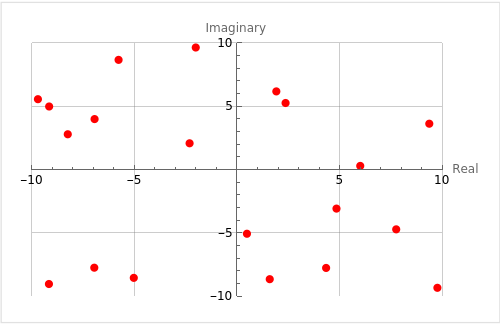
\includegraphics{complexplane.png}
    \caption{Complex Plane}
\end{figure}

\begin{definition}[Complex Plane]
    The complex plane is a two-dimensional space where each point represents a complex number. The horizontal axis represents the real part of the number, and the vertical axis represents the imaginary part. This allows for a geometric interpretation of complex numbers.
\end{definition}
Now that we have point representation on the complex plane, we can gauge the length of a complex number, which we call
\textbf{absolute value} or \textbf{modulus}, as what we do to vectors.
\begin{definition}[Modulus of Complex Number]
    The absolute value or modulus of the number \( z = a + bi \) is denoted by \( |z| \) and is given by
\[ |z| := \sqrt{a^2 + b^2}. \]
\end{definition}
In particular,
\[ |0| = 0, \quad \left|\frac{i}{2}\right| = \frac{1}{2}, \quad |3 - 4i| = \sqrt{9 + 16} = 5. \]
Similarly, we can also gain the distance between two complex numbers in the plane by taking them as two points.
\begin{definition}[Distance between Complex Number]
    Let \( z_1 = a_1 + b_1i \) and \( z_2 = a_2 + b_2i \). 
    \begin{equation}
        |z_1 - z_2| = |(a_1 - a_2) + (b_1 - b_2)i| = \sqrt{(a_1 - a_2)^2 + (b_1 - b_2)^2}
    \end{equation}
\end{definition}
We can use this property to describe curves in the plane.
\begin{example}
    Draw the area that satisfies $|z-z_0|=1$, where $z_0 = 2+2i$.
\end{example}

This set consists of all points $z$ whose distance from $z_0$ is $r$.
\begin{figure}[H]
    \centering
    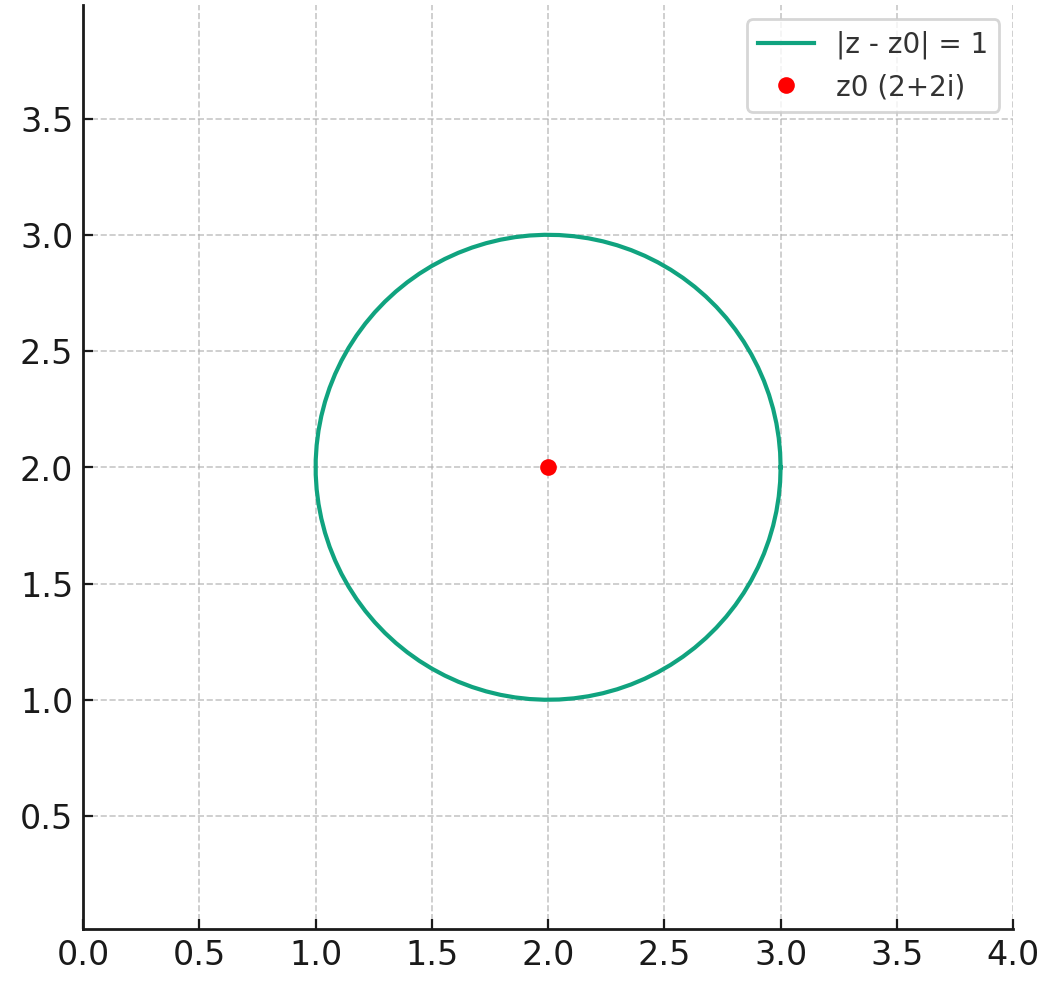
\includegraphics[width = 0.5\textwidth]{locus1.png}
\end{figure}
\begin{example}
    Describe the set of points \( z \) that satisfy the equations

\begin{enumerate}
\item[(a)] \( |z + 2| = |z - 1| \),
\item[(b)] \( |z - 1| = \text{Re} \, z + 1 \).
\end{enumerate}
\end{example}
\textbf{Solution.}

\begin{itemize}
    \item[(a)] A point \( z \) satisfies Eq. (a) if and only if it is equidistant from the points \( -2 \) and \( 1 \). Hence, Eq. (a) is the equation of the perpendicular bisector of the line segment joining \( -2 \) and \( 1 \); that is, Eq. (a) describes the line \( x = -\frac{1}{2} \).

    A more routine method for solving Eq. (a) is to set \( z = x + iy \) in the equation and perform the algebra:
    \begin{align*}
        |z + 2| &= |z - 1|, \\
        |x + iy + 2| &= |x + iy - 1|, \\
        (x + 2)^2 + y^2 &= (x - 1)^2 + y^2, \\
        4x + 4 &= -2x + 1, \\
        x &= -\frac{1}{2}.
    \end{align*}

    \item[(b)] The geometric interpretation of Eq. (b) is less obvious, so we proceed directly with the mechanical approach and derive
    $$\sqrt{(x-1)^2} + y^2 = x+1 \iff y^2 = 4x$$
    which is a parabola.
\end{itemize}
Another important concept is \textbf{complex conjugate}.

Geometrically, the conjugate of a complex number is its reflection on the x-axis.
\begin{wrapfigure}{r}{0.5\textwidth}
    \centering
    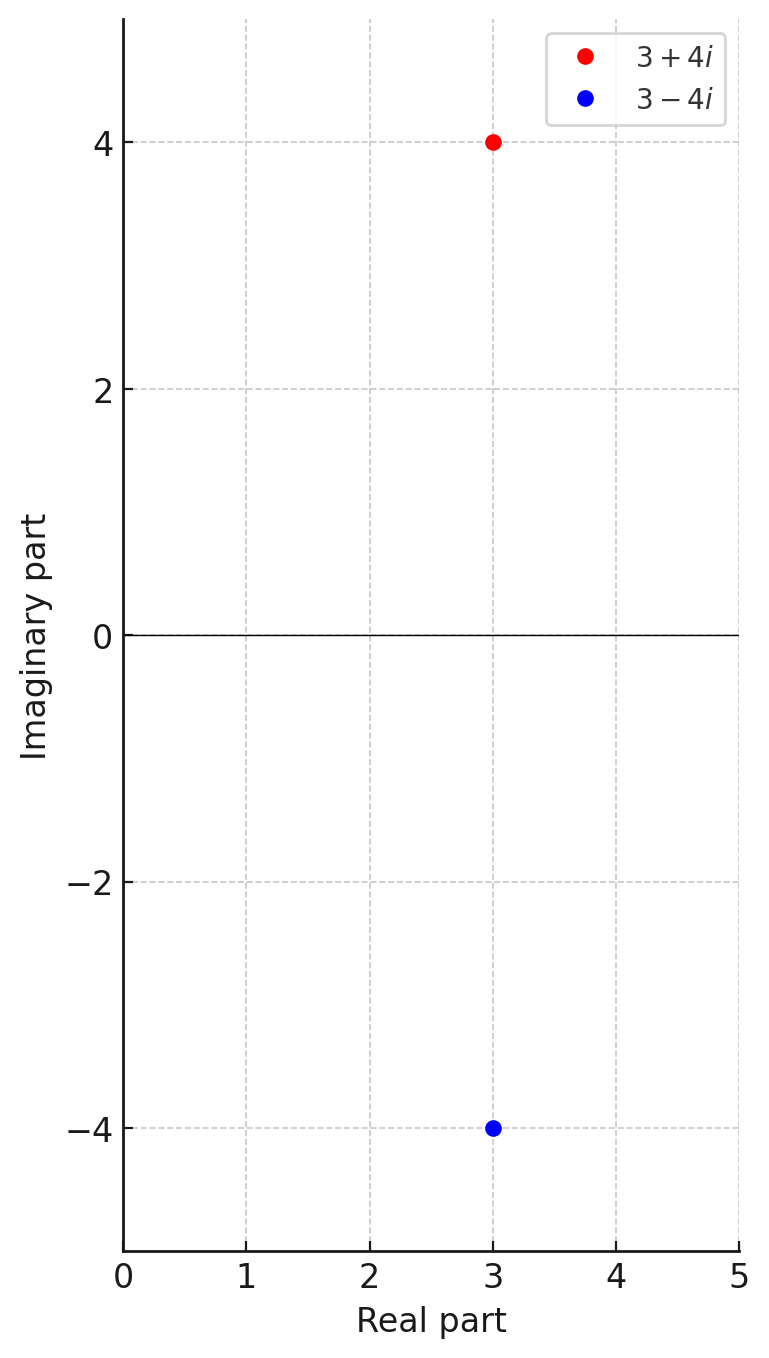
\includegraphics[width=0.48\textwidth]{conjugate.png}
    \caption{Complex Conjugate}
  \end{wrapfigure}
  The complex conjugate of the number $z = a+bi$ is denoted by $\bar{z} = a-bi $.
  It follows that \( z = \bar{z} \) if and only if \( z \) is a real number. Also, it is clear that the conjugate of the sum (difference) of two complex numbers is equal to the sum (difference) of their conjugates; that is,

$$z_1 + z_2 = \bar{z}_1 + \bar{z}_2$$

$$\quad z_1 - z_2 = \bar{z}_1 - \bar{z}_2$$

We also have:
$$\bar{(z_1z_2)} = \bar{z_1} \bar{z_2}$$
and
$$\begin{aligned}\overline{\left(\frac{z_1}{z_2}\right)}&=\frac{\bar{z_1}}{\bar{z_2}}\quad(z_2\neq0);\\\operatorname{Re}z&=\frac{z+\bar{z}}2;\\\operatorname{Im}z&=\frac{z-\bar{z}}{2i};\end{aligned}$$
The proof is not very complex, and is therefore exercises for this section.
\\
\subsection{Exercises}


\begin{exercise}
    Describe the set of points \( z \) in the complex plane that satisfies each of the following.
    \begin{enumerate}
        \item[\textbf{(a)}] \( \text{Im} \, z = -2 \)
        \item[\textbf{(b)}] \( |z - 1 + i| = 3 \)
        \item[\textbf{(c)}] \( |2z - i| = 4 \)
        \item[\textbf{(d)}] \( |z - 1| = |z + i| \)
        \item[\textbf{(e)}] \( |z| = \text{Re} \, z + 2 \)
        \item[\textbf{(f)}] \( |z - 1| + |z + 1| = 7 \)
        \item[\textbf{(g)}] \( |z| = 3|z - 1| \)
        \item[\textbf{(h)}] \( \text{Re} \, z \geq 4 \)
        \item[\textbf{(i)}] \( |z - i| < 2 \)
        \item[\textbf{(j)}] \( |z| > 6 \)
      \end{enumerate}
\end{exercise}
\begin{proof}
    Here we describe the set of points \( z \) in the complex plane that satisfies each of the following conditions:
    
    \begin{enumerate}
      \item[\textbf{(a)}] For \( \text{Im} \, z = -2 \), the Cartesian equation is \( y = -2 \).
      \item[\textbf{(b)}] For \( |z - 1 + i| = 3 \), the Cartesian equation is \( (x - 1)^2 + (y + 1)^2 = 9 \).
      \item[\textbf{(c)}] For \( |2z - i| = 4 \), the Cartesian equation is \( (2x)^2 + (2y - 1)^2 = 16 \).
      \item[\textbf{(d)}] For \( |z - 1| = |z + i| \), the Cartesian equation is \( (x - 1)^2 + y^2 = x^2 + (y + 1)^2 \).
      \item[\textbf{(e)}] For \( |z| = \text{Re} \, z + 2 \), the Cartesian equation is \( x^2 + y^2 = x + 2 \).
      \item[\textbf{(f)}] For \( |z - 1| + |z + 1| = 7 \), this is the equation of an ellipse with foci at (1,0) and (-1,0).
      \item[\textbf{(g)}] For \( |z| = 3|z - 1| \), the Cartesian equation is \( x^2 + y^2 = 3(\sqrt{(x - 1)^2 + y^2}) \).
      \item[\textbf{(h)}] For \( \text{Re} \, z \geq 4 \), the Cartesian equation is \( x \geq 4 \).
      \item[\textbf{(i)}] For \( |z - i| < 2 \), the Cartesian equation is \( (x)^2 + (y - 1)^2 < 4 \).
      \item[\textbf{(j)}] For \( |z| > 6 \), the Cartesian equation is \( x^2 + y^2 > 36 \).
    \end{enumerate}
    \end{proof}

    \begin{exercise}
        Prove that if \( \overline{z}^2 = z^2 \), then \( z \) is either real or pure imaginary.
        \end{exercise}
        
        \begin{proof}
        Let \( z = a + bi \) where \( a \) and \( b \) are real numbers and \( i \) is the imaginary unit. Then \( \overline{z} = a - bi \). 
        
        According to the premise:
        \[ \overline{z}^2 = (a - bi)^2 = a^2 - 2abi + b^2i^2 = a^2 - 2abi - b^2 \]
        \[ z^2 = (a + bi)^2 = a^2 + 2abi + b^2i^2 = a^2 + 2abi - b^2 \]
        
        For \( \overline{z}^2 \) to equal \( z^2 \), the real parts and the imaginary parts of \( \overline{z}^2 \) and \( z^2 \) must be equal, thus:
        \[ a^2 - b^2 = a^2 - b^2 \]
        \[ -2ab = 2ab \]
        
        The real parts are already equal. For the imaginary parts to be equal, \( -2ab \) must equal \( 2ab \), which is only possible if \( ab = 0 \). This means that either \( a = 0 \) or \( b = 0 \) (or both).
        
        If \( a = 0 \), then \( z \) is pure imaginary. If \( b = 0 \), then \( z \) is real. Hence, if \( \overline{z}^2 = z^2 \), \( z \) must be either real or pure imaginary.
        \end{proof}

        \begin{exercise}
            Show that:
            \begin{itemize}
                \item$\lvert z_1z_2 \rvert = \lvert z_1 \rvert \lvert z_2 \rvert$ \quad (the modulus of a product is the product of the moduli)
                \item $\left\lvert \frac{z_1}{z_2} \right\rvert = \frac{\lvert z_1 \rvert}{\lvert z_2 \rvert}$ \quad (the modulus of a quotient is the quotient of the moduli)
                \item $\lvert z_1 \rvert + \lvert z_2 \rvert \leq \lvert z_1 + z_2 \rvert$ \quad (triangle inequality)
              \end{itemize}
        \end{exercise}
        
        \begin{exercise}
            Show that:
            \begin{itemize}
                \item $z_1 + z_2 = \overline{z_1} + \overline{z_2}$
                \item $z_1z_2 = \overline{z_1} \, \overline{z_2}$
                \item $\overline{z}z = \lvert z \rvert^2$
                \item $z + \overline{z} = 2Re(z)$
                \item $kz = \overline{kz}$, for $k \in \mathbb{R}$
              \end{itemize}
        \end{exercise}
        \begin{exercise}
            Prove that \( \overline{z}^k = (\overline{z^k}) \) for every integer \( k \) (provided \( z \neq 0 \) when \( k \) is negative).
            \end{exercise}
            
            \begin{proof}
            Consider a complex number \( z = a + bi \), where \( a \) and \( b \) are real numbers and \( i \) is the imaginary unit. The complex conjugate of \( z \) is \( \overline{z} = a - bi \).
            
            The statement is trivially true for \( k = 0 \) and \( k = 1 \). Now let \( k \) be any positive integer.
            
            We proceed by induction on \( k \):
            
            \textbf{Base case} (\( k = 1 \)):
            \[ \overline{z}^1 = \overline{z} = a - bi = \overline{z^1} \]
            The base case holds.
            
            \textbf{Inductive step}:
            Assume the statement is true for \( k \), i.e., \( \overline{z}^k = \overline{z^k} \). We need to show that \( \overline{z}^{k+1} = \overline{z^{k+1}} \).
            \[ \overline{z}^{k+1} = \overline{z}^k \cdot \overline{z} = \overline{z^k} \cdot \overline{z} \]
            Using the property of complex conjugates that \( \overline{zw} = \overline{z} \cdot \overline{w} \), we have:
            \[ \overline{z^k} \cdot \overline{z} = \overline{z^k \cdot z} = \overline{z^{k+1}} \]
            This completes the inductive step.
            
            For negative integers \( k \), we have \( \overline{z}^k = \overline{z^{-k}} = (\overline{z^{-1}})^k = (\overline{z})^k \), since the complex conjugate of a reciprocal is the reciprocal of the complex conjugate, and the induction hypothesis applies.
            
            Therefore, \( \overline{z}^k = (\overline{z^k}) \) for every integer \( k \).
            \end{proof}

            \begin{exercise}\label{conjugate root}
                Let \( a_1, a_2, \ldots, a_n \) be real constants. Show that if \( z_0 \) is a root of the polynomial equation \( z^n + a_1z^{n-1} + a_2z^{n-2} + \ldots + a_n = 0 \), then so is \( \overline{z_0} \).
                \end{exercise}
                
                \begin{proof}
                Suppose \( z_0 \) is a root of the polynomial \( P(z) = z^n + a_1z^{n-1} + a_2z^{n-2} + \ldots + a_n \). This means that:
                \[ P(z_0) = z_0^n + a_1z_0^{n-1} + a_2z_0^{n-2} + \ldots + a_n = 0 \]
                
                Taking the complex conjugate of the entire equation, we have:
                \[ \overline{P(z_0)} = \overline{z_0^n + a_1z_0^{n-1} + a_2z_0^{n-2} + \ldots + a_n} = \overline{0} \]
                
                Since the \( a_i \) are real, \( \overline{a_i} = a_i \), and using the property that \( \overline{z + w} = \overline{z} + \overline{w} \) and \( \overline{zw} = \overline{z}\cdot \overline{w} \), we get:
                \[ \overline{P(z_0)} = \overline{z_0}^n + a_1\overline{z_0}^{n-1} + a_2\overline{z_0}^{n-2} + \ldots + a_n \]
                
                Since \( \overline{0} = 0 \), the equation simplifies to:
                \[ P(\overline{z_0}) = \overline{z_0}^n + a_1\overline{z_0}^{n-1} + a_2\overline{z_0}^{n-2} + \ldots + a_n = 0 \]
                
                Therefore, \( \overline{z_0} \) is also a root of the polynomial \( P(z) \).
                \end{proof}
                \begin{remark}
                    This statement is actually \textbf{Conjugate Root Theorem}, which we will discuss further details about in finding
                    complex roots of equations.
                \end{remark}
            \begin{exercise}
                We have noted that the conjugate \( \overline{z} \) is the reflection of the point \( z \) in the real axis (the horizontal line \( y = 0 \)). Show that the reflection of \( z \) in the line \( ax + by = c \) (where \( a, b, c \) are real) is given by
\[ \frac{2ic    + (b - ai)\overline{z}}{b + ai} \]
            \end{exercise}
            Hint: In general, the reflection of the point \( (x_1, y_1) \) in the line \( ax + by + c = 0 \) given by this formula:
            \[ 
            x_2 = \frac{x_1(b^2 - a^2) - 2aby_1 - 2ac}{a^2 + b^2}
            \]
            \[ 
            y_2 = \frac{y_1(a^2 - b^2) - 2abx_1 - 2bc}{a^2 + b^2}
            \]
            
            \begin{proof}
                Now the reflection of $z = (x, y)$ in the line $ax + by - c = 0$ is $w = u + iv$, $u, v \in \mathbb{R}$, where:
                \begin{align*}
                u &= \frac{x(b^2 - a^2) - 2aby + 2ac}{a^2 + b^2}, \\
                v &= \frac{y(a^2 - b^2) - 2abx + 2bc}{a^2 + b^2}.
                \end{align*}
                Then:
                \begin{align*}
                w = u + vi &= \frac{x(b^2 - a^2) - 2aby + 2ac}{a^2 + b^2} + \frac{y(a^2 - b^2) - 2abx + 2bc}{a^2 + b^2}i. 
                \end{align*}
                Next, we'll prove now:
                \begin{align*}
                w &= \frac{2ic + (b - ai)\overline{z}}{b + ai}.
                \end{align*}
                We'll factorize and simplify $w$ in $(*)$:
                \begin{align*}
                w &= \frac{x(b^2 - a^2) - 2aby + 2ac}{a^2 + b^2} + \frac{y(a^2 - b^2) - 2abx + 2bc}{a^2 + b^2}i \\
                &= \frac{x(b^2 - a^2) - 2aby + 2ac + y(a^2 - b^2)i - 2abxi + 2bci}{a^2 + b^2}.
                \end{align*}
                Simplify more:
                \begin{align*}
                (b^2 - a^2 - 2abi) &= (b - ai)^2, \\
                (a^2i - b^2i - 2ab) &= (-i)(b^2 - a^2 + 2ab) \\
                &= (-i)(b + ai)^2 \quad \left(\text{since } \frac{1}{i} = -i\right), \\
                &= (-i)(b - ai)(b + ai)^2 \\
                &= i(b - ai) \\
                &= i(b - ai)(b + ai).
                \end{align*}
                Now we'll put all of them in the $(1)$,
                \begin{align*}
                w &= \frac{x(b - ai)^2 - yi(b - ai)^2 + 2ci(b - ai)}{b + ai} \\
                &= \frac{(b - ai)x(b - ai) - yi(b - ai) + 2ci}{b + ai} \\
                &= \frac{2ci + (b - ai)\overline{z}}{b + ai}.
                \end{align*}
                Therefore, the reflection of $z$ in the line $ax + by = c$ is:
                \begin{align*}
                w &= \frac{2ic + (b - ai)\overline{z}}{b + ai}.
                \end{align*}
                \end{proof}
               
\section{Vector and Polar Form}
\subsection{Vector Form of Complex Number}
Now that we can express complex numbers as points scattered in the complex plane, we can take them as direction vectors
in the plane as shown in figure \ref{vec}. 
\begin{figure}[H]
    \centering \label{vec}
    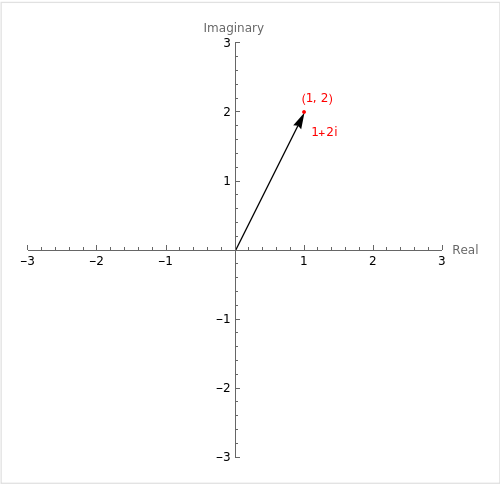
\includegraphics[width = 0.5\textwidth]{complexvector.png}
    \caption{Complex Number as Vector}
\end{figure}
With this, we can apply all possible operations of vectors to complex numbers, such as the \textbf{parallelogram law} as in figure \ref{parrl}.
\begin{figure}[H]
    \centering \label{parrl}
    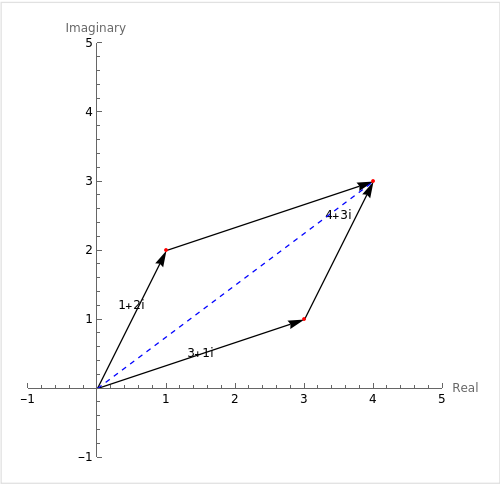
\includegraphics[width = 0.5\textwidth]{paralaw.png}
    \caption{Parallelogram Law}
\end{figure}
Examing this figure, it actually reminds us of a important conclusion mentioned in earlier chapter. If we focus on
the lower triangle of the parallelogram, and denote these two complex numbers as $z_1$ and $z_2$ respectively.
They hold that: $$|z_1+z_2| \leq |z_1|+|z_2|$$
This is exactly the geometrical meaning of triangular inequality as in definition \ref{triangularineq}.
And these are all we need to know about complex number's vector form, as it is not used very common.

\subsection{Polar Form of Complex Number}
This section discusses one of the most commonly used form of complex number. We start with introducing a new coordinate syste.

\subsubsection{The Polar Coordinate}
Polar coordinates provide an alternative to Cartesian coordinates for describing the location of points in a two-dimensional plane. While Cartesian coordinates use a grid of horizontal and vertical lines to specify a point by its horizontal (x) and vertical (y) distances from an origin, polar coordinates specify a point by its distance from a reference point (called the pole, analogous to the origin) and an angle relative to a reference direction.
\begin{figure}[H]
    \centering \label{polar}
    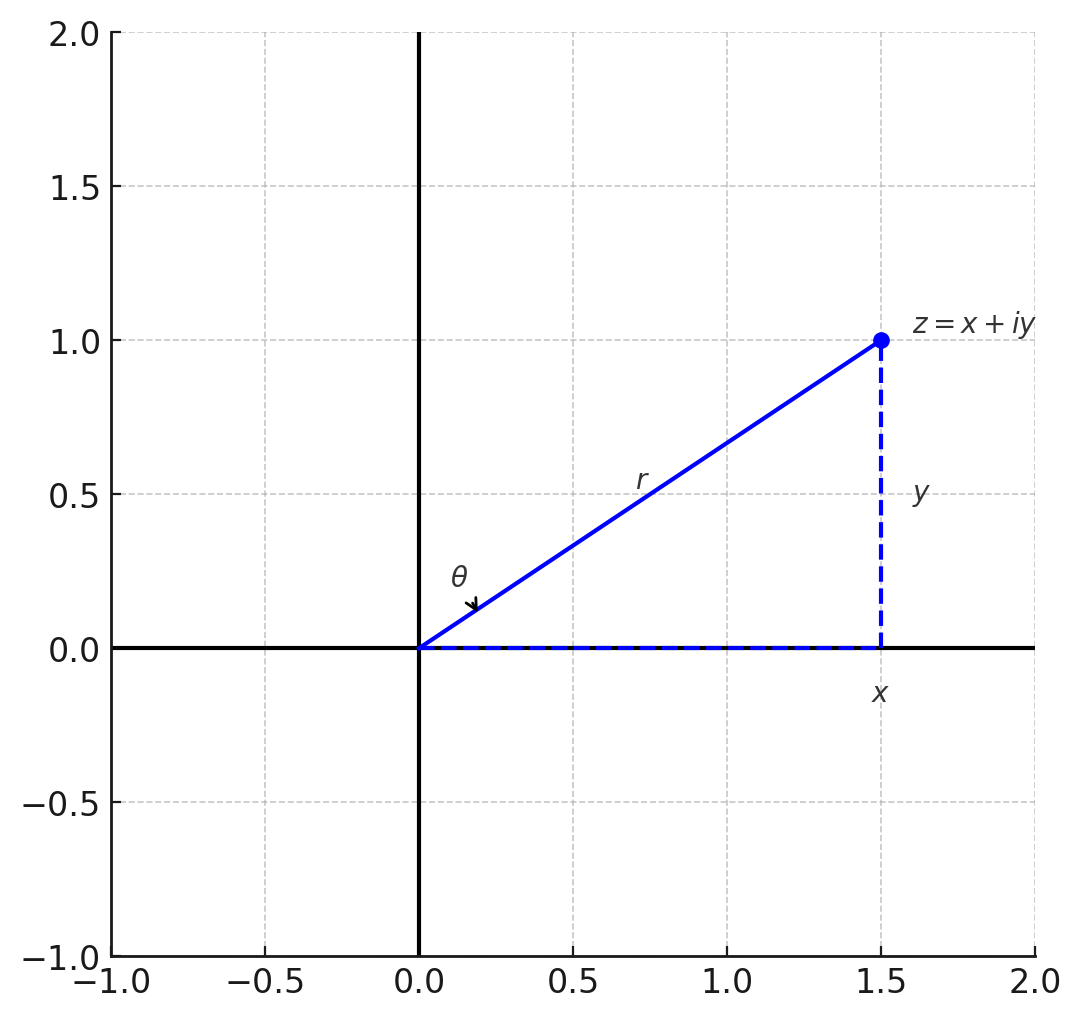
\includegraphics[width = 0.5\textwidth]{polar2.png}
    \caption{Complex Number in Polar Coordinate}
\end{figure}
A point's location in polar coordinates is given as \( (r, \theta) \), where \( r \) is the radial distance from the pole, and \( \theta \) is the angular coordinate, typically measured in radians from the positive x-axis (the reference direction). Polar coordinates are particularly useful in situations where the geometry of a problem has rotational symmetry, making it more natural and simpler to work with angles and radii than with rectangular coordinates.

One of the most common applications of polar coordinates is in the field of trigonometry, complex numbers, and vector calculus, where they provide a more straightforward approach to solving problems involving circular motion, periodic functions, and fields.

\subsubsection{Polar Expression of Complex Number}
Now that we know the existence of polar form, how can we get it from Cartesian form? In the Cartesian coordinate,
the positions are expressed, straightforwardly, in the horizontal and vertical distance to y and x-axis, while in polar
coordinate, we express them using the angle between the line from the origin to the specific position and the horizontal axis, as well
as the length of this line. Is there a mapping or relation between the points in these two types of coordinates? Some clever students
may have noticed that trigonometric functions are the keys here.
we readily derive the equations expressing the rectangular (or Cartesian) coordinates $(x, y)$ in terms of the polar coordinates $(r, \theta)$:
\begin{equation}
x = r \cos \theta, \quad y = r \sin \theta. 
\end{equation}
On the other hand, the expressions for $(r, \theta)$ in terms of $(x, y)$ contain some minor but troublesome complications. Indeed the coordinate $r$ is given, unambiguously, by
\begin{equation}
r = \sqrt{x^2 + y^2} = |z|. 
\end{equation}

However, observe that although it is certainly true that $\tan \theta = \frac{y}{x}$, the natural conclusion
\begin{equation}
\theta = \tan^{-1}\left(\frac{y}{x}\right)
\end{equation}
is \textit{invalid} for points $z$ in the second and third quadrants (since the standard interpretation of the arctangent function places its range in the first and fourth quadrants). Since an angle is fixed by its sine \textit{and} cosine, $\theta$ is uniquely determined by the pair of equations
\begin{equation}
\cos \theta = \frac{x}{|z|}, \quad \sin \theta = \frac{y}{|z|}, 
\end{equation}
And all these lead us to the polar form of a given complex number:
\begin{equation}
    z=x+iy=r(\cos\theta+i\sin\theta)=r\operatorname{cis}\theta
\end{equation}

Considering the circularity of radiant, we introduce the \textbf{argument} of complex number.
\begin{definition}[Arguement of Complex Number] \label{polarform}
In the study of complex numbers, the \emph{argument} of a complex number \( z \), denoted as \( \text{arg}(z) \), is a fundamental concept representing the angle between the positive real axis and the line segment that joins the origin with the point \( z \) in the complex plane. Specifically, if \( z = x + iy \), where \( x \) and \( y \) are real numbers, then \( \text{arg}(z) \) is defined as the angle \( \theta \) in polar coordinates that satisfies \( x = r\cos(\theta) \) and \( y = r\sin(\theta) \), where \( r \) is the magnitude of \( z \). The value of \( \text{arg}(z) \) is usually given in radians and, by convention, is restricted to the interval \( (-\pi, \pi] \), known as the principal value. The argument provides a complete description of the direction in which the point \( z \) lies from the origin, serving as a crucial tool in the fields of complex analysis, phasor calculus in electrical engineering, and in the representation of waves and oscillations.
\end{definition}

\begin{example}
    Find $\arg(1 + \sqrt{3}i)$ and write $1 + \sqrt{3}i$ in polar form.
\end{example}
\textbf{Solutions:}

Note that $r = |1 + \sqrt{3}i| = 2$ and that the equations $\cos\theta = \frac{1}{2}$, $\sin\theta = \frac{\sqrt{3}}{2}$ are satisfied by $\theta = \frac{\pi}{3}$. Hence $\arg(1 + \sqrt{3}i) = \frac{\pi}{3} + 2k\pi, k = 0, \pm1, \pm2, \ldots$ [in particular, $\text{Arg}(1 + \sqrt{3}i) = \frac{\pi}{3}$]. The polar form of $1 + \sqrt{3}i$ is
\[2(\cos\frac{\pi}{3} + i\sin\frac{\pi}{3}) = 2\operatorname{cis}\frac{\pi}{3}.\]

More properties of polar form complex number could be derived with properties of trigonometric identities.
Now suppose we have 
$$z_1=r_1\left(\cos\theta_1+i\sin\theta_1\right),\quad z_2=r_2\left(\cos\theta_2+i\sin\theta_2\right)$$
then we have
$$z_1z_2=r_1r_2\left[(\cos\theta_1\cos\theta_2-\sin\theta_1\sin\theta_2)+i(\sin\theta_1\cos\theta_2+\cos\theta_1\sin\theta_2)\right]$$
which follows that
\begin{equation} \label{polarprod}
    z_1z_2=r_1r_2\left[\cos\left(\theta_1+\theta_2\right)+i\sin\left(\theta_1+\theta_2\right)\right]
\end{equation}

\begin{remark}
The compound angle formula is applied in the proof, which should already been covered in high school
syllabus. You may refer to \href{https://en.wikipedia.org/wiki/List_of_trigonometric_identities}{this link} for further information.
A concise proof is provided below.
\begin{proof}[Proof of the Composite Angle Formulas]
    To prove the sine of the sum of two angles \( \alpha \) and \( \beta \), we can use the unit circle and the definition of sine and cosine.
    
    Consider a unit circle where point \( A \) corresponds to angle \( \alpha \), and point \( B \) corresponds to angle \( \alpha + \beta \). Point \( A \) has coordinates \( (\cos(\alpha), \sin(\alpha)) \), and point \( B \) has coordinates \( (\cos(\alpha + \beta), \sin(\alpha + \beta)) \).
    
    By rotating point \( A \) by angle \( \beta \), we can form a right triangle where the new point, \( C \), has coordinates \( (\cos(\alpha)\cos(\beta) - \sin(\alpha)\sin(\beta), \sin(\alpha)\cos(\beta) + \cos(\alpha)\sin(\beta)) \).
    
    The coordinates of point \( C \) represent the cosine and sine of the sum of angles \( \alpha \) and \( \beta \) due to the rotation. Therefore, we have:
    
    \[
    \sin(\alpha + \beta) = \sin(\alpha)\cos(\beta) + \cos(\alpha)\sin(\beta)
    \]
    \[
    \cos(\alpha + \beta) = \cos(\alpha)\cos(\beta) - \sin(\alpha)\sin(\beta)
    \]
    
    Similarly, by considering the rotation in the opposite direction (subtracting angle \( \beta \) from \( \alpha \)), we can derive the formulas for the sine and cosine of the difference of two angles:
    
    \[
    \sin(\alpha - \beta) = \sin(\alpha)\cos(\beta) - \cos(\alpha)\sin(\beta)
    \]
    \[
    \cos(\alpha - \beta) = \cos(\alpha)\cos(\beta) + \sin(\alpha)\sin(\beta)
    \]
    
    Thus, we have proven the composite angle formulas for sine and cosine.

    \end{proof}
\end{remark}

The abbreviated version of Eq. \ref{polarprod} reads as follows:
\[
\overline{z_1z_2} = (r_1 \operatorname{cis} \theta_1)(r_2 \operatorname{cis} \theta_2) = (r_1r_2) \operatorname{cis} (\theta_1 + \theta_2)
\]
and we see that

\textbf{The modulus of the product is the product of the moduli:}
\[
|\overline{z_1z_2}| = |z_1||z_2| \quad (= r_1r_2);
\]


\textbf{The argument of the product is the sum of the arguments:}
\[
\arg \overline{z_1z_2} = \arg z_1 + \arg z_2 \quad (= \theta_1 + \theta_2).
\]
As division is the inverse of multiplication, we can get the following statements by similar method:
\begin{equation} \label{5.8}
    \frac{z_{1}}{z_{2}}=\frac{r_{1}}{r_{2}}\left[\cos\left(\theta_{1}-\theta_{2}\right)+i\sin\left(\theta_{1}-\theta_{2}\right)\right]=\frac{r_{1}}{r_{2}}\mathrm{cis}\left(\theta_{1}-\theta_{2}\right)
\end{equation}
\begin{equation}\label{5.9}
    \arg\left(\frac{z_{1}}{z_{2}}\right)=\arg z_{1}-\arg z_{2} 
\end{equation}
\begin{equation}\label{5.10}
    \left|\frac{z_1}{z_2}\right|=\frac{|z_1|}{|z_2|}
\end{equation}
\begin{example}
    Write the quotient \( \frac{(1 + i)}{(\sqrt{3} - i)} \) in polar form.
\end{example}
\begin{proof}
    The polar forms for \( 1 + i \) and \( \sqrt{3} - i \) are
    \[
    1 + i = |1 + i| \operatorname{cis}(\arg(1 + i)) = \sqrt{2} \operatorname{cis}\left(\frac{\pi}{4}\right),
    \]
    \[
    \sqrt{3} - i = 2 \operatorname{cis}\left(-\frac{\pi}{6}\right).
    \]
    Hence, from Eq. \ref{5.8}, we have
    \[
    \frac{1 + i}{\sqrt{3} - i} = \frac{\sqrt{2}}{2} \operatorname{cis} \left(\frac{\pi}{4} - \left(-\frac{\pi}{6}\right)\right) = \frac{\sqrt{2}}{2} \operatorname{cis}\left(\frac{5\pi}{12}\right).
    \]
    \end{proof}

\subsection{Exercises}
\begin{exercise}
    Find the following:
    \begin{enumerate}
        \item[(a)] \( \left| \frac{1 + 2i}{-2 - i} \right| \)
        \item[(b)] \( \left| (1 + i)(2 - 3i)(4i - 3) \right| \)
        \item[(c)] \( \left| \frac{i(2 + i)^3}{(1 - i)^2} \right| \)
        \item[(d)] \( \left| \frac{(\pi + i)^{100}}{(\pi - i)^{100}} \right| \)
    \end{enumerate}
\end{exercise}
\begin{exercise}
    Draw the following vectors:
    \begin{enumerate}
        \item[(a)] \( 7 \operatorname{cis}\left(\frac{3\pi}{4}\right) \)
        \item[(b)] \( 4 \operatorname{cis}\left(-\frac{\pi}{6}\right) \)
        \item[(c)] \( \operatorname{cis}\left(\frac{3\pi}{4}\right) \)
        \item[(d)] \( 3 \operatorname{cis}\left(\frac{27\pi}{4}\right) \)
    \end{enumerate}
\end{exercise}
\begin{exercise}
    Find the argument of each of the following complex numbers and write each in polar form:
    \begin{enumerate}
        \item[(a)] \( -\frac{1}{2} \)
        \item[(b)] \( -3 + 3i \)
        \item[(c)] \( -\pi i \)
        \item[(d)] \( -2\sqrt{3} - 2i \)
        \item[(e)] \( (1 - i)(-\sqrt{3} + i) \)
        \item[(f)] \( (\sqrt{3} - i)^2 \)
        \item[(g)] \( \frac{-1 + \sqrt{3}i}{2 + 2i} \)
        \item[(h)] \( \frac{-\sqrt{7}(1 + i)}{\sqrt{3} + i} \)
    \end{enumerate}
\end{exercise}
\begin{exercise}
    Show geometrically that the nonzero complex numbers \( z_1 \) and \( z_2 \) satisfy \( z_1 + z_2 = |z_1| + |z_2| \) if and only if they have the same argument.
\end{exercise}
\begin{proof}
    If \( z_1 \) and \( z_2 \) have the same argument, it follows that:

    We see here if $z_1 = r_1(\cos \theta + i \sin \theta)$, $z_2 = r_2(\cos \theta + i \sin \theta)$, then
\begin{align*}
|z_1 + z_2| &= |r_1(\cos \theta + i \sin \theta) + r_2(\cos \theta + i \sin \theta)| \\
&= |(r_1 + r_2)(\cos \theta + i \sin \theta)| \\
&= r_1 + r_2 = |z_1| + |z_2|
\end{align*}
\end{proof}
\begin{exercise}
    Given the vector \( z \), interpret geometrically the vector \( (\cos \phi + i \sin \phi)z \).
\end{exercise}
\textbf{Solution:}

Let \( z \in \mathbb{C} \), \( z = r(\cos \theta + i \sin \theta) \)

\[
(\cos \phi + i \sin \phi)z = (\cos \phi + i \sin \phi)r(\cos \theta + i \sin \theta)
\]
\[
= r[\cos(\theta + \phi) + i \sin(\theta + \phi)]
\]
\[
= r\operatorname{cis}(\theta + \phi)
\]

Geometrically this: \( r\operatorname{cis}(\theta + \phi) \) means a vector that its length \( r \) and argument is \( \theta + \phi \), we can get it by rotating vector \( z \) about origin through an angle \( \phi \) in the counterclockwise direction.

\begin{exercise}
    Show that $|z_1z_2z_3|=|z_1||z_2||z_3|$ and thus prove 
    $$|\prod_{i=1}^{n} z_i| = \prod_{i=1}^{n} |z_i|$$
    \begin{remark}
        $\prod$ is called pi (upper case) notation. Take it as the sigma notation for multiplication.
    \end{remark}
\end{exercise}
    \begin{proof}
        Consider the complex numbers \( z_1 = r_1(\cos \theta_1 + i\sin \theta_1) \), \( z_2 = r_2(\cos \theta_2 + i\sin \theta_2) \), and \( z_3 = r_3(\cos \theta_3 + i\sin \theta_3) \), where \( r_1, r_2, \) and \( r_3 \) are the moduli of \( z_1, z_2, \) and \( z_3 \) respectively, and \( \theta_1, \theta_2, \) and \( \theta_3 \) are the arguments. The product \( z_1z_2z_3 \) is then given by:
        \[
        z_1z_2z_3 = r_1r_2r_3(\cos(\theta_1 + \theta_2 + \theta_3) + i\sin(\theta_1 + \theta_2 + \theta_3))
        \]
        
        The modulus of this product is:
        \[
        |z_1z_2z_3| = |r_1r_2r_3(\cos(\theta_1 + \theta_2 + \theta_3) + i\sin(\theta_1 + \theta_2 + \theta_3))| = r_1r_2r_3
        \]
        
        Since the moduli of \( z_1, z_2, \) and \( z_3 \) are \( r_1, r_2, \) and \( r_3 \) respectively, it follows that:
        \[
        |z_1z_2z_3| = |z_1||z_2||z_3|
        \]
        
        Now, extend this property to a product of \( n \) complex numbers:
        \[
        \prod_{i=1}^{n} z_i = \prod_{i=1}^{n} r_i(\cos \theta_i + i\sin \theta_i)
        \]
        
        Taking the modulus of both sides:
        \[
        \left|\prod_{i=1}^{n} z_i\right| = \left|\prod_{i=1}^{n} r_i(\cos \theta_i + i\sin \theta_i)\right| = \prod_{i=1}^{n} r_i
        \]
        
        Thus:
        \[
        \prod_{i=1}^{n} |\overline{z_i}| = \prod_{i=1}^{n} |z_i|
        \]
        
        as required.

        MI is also a option:

        \textbf{Base case} (\(n = 1\)): For a single complex number \(z_1\), the statement is trivially true since \(|\overline{z_1}| = |z_1|\).

        \textbf{Inductive step}: Assume the statement holds for \(n = k\), i.e.,
        \[
        \prod_{i=1}^{k} |\overline{z_i}| = \prod_{i=1}^{k} |z_i|
        \]
        Now consider \(n = k + 1\) complex numbers. By the induction hypothesis and the property that the modulus of a product is equal to the product of the moduli for any two complex numbers \(a\) and \(b\), namely \(|ab| = |a||b|\), we have:
        \[
        \prod_{i=1}^{k+1} |\overline{z_i}| = |\overline{z_{k+1}}| \prod_{i=1}^{k} |\overline{z_i}| = |z_{k+1}| \prod_{i=1}^{k} |z_i| = \prod_{i=1}^{k+1} |z_i|
        \]
        Thus, by mathematical induction, the statement is proved for all \(n \in \mathbb{N}\).
        \end{proof}

    \begin{exercise}
        Show that\begin{enumerate}
            \item[(a)] $\text{arg } z_1z_2z_3 = \text{arg } z_1 + \text{arg } z_2 + \text{arg } z_3$
            \item[(b)] $\text{arg } z_1 \overline{z_2} = \text{arg } z_1 - \text{arg } z_2$.
        \end{enumerate}
    \end{exercise}              
    \textbf{Solution:}
    Let $z_1, z_2, z_3 \in \mathbb{C}$,

(a) we'll prove $\text{arg }(z_1z_2z_3) = \text{arg } z_1 + \text{arg } z_2 + \text{arg } z_3$

Let $z_1 = r_1(\cos \theta_1 + i \sin \theta_1)$, where $\text{arg } z_1 = \theta_1$

$z_2 = r_2(\cos \theta_2 + i \sin \theta_2)$, where $\text{arg } z_2 = \theta_2$

$z_3 = r_3(\cos \theta_3 + i \sin \theta_3)$, where $\text{arg } z_3 = \theta_3$

We'll prove $\text{arg } z_1z_2z_3 = \text{arg } z_1 + \text{arg } z_2 + \text{arg } z_3$

At first we'll find $z_1z_2z_3$:

\begin{align*}
    z_1z_2z_3 &= (z_1z_2)z_3 = r_1r_2[\cos(\theta_1 + \theta_2) + i \sin(\theta_1 + \theta_2)]z_3 \\
    &= r_1r_2r_3[\cos(\theta_1 + \theta_2) + i \sin(\theta_1 + \theta_2)](\cos \theta_3 + i \sin \theta_3) \\
    &= r_1r_2r_3[\cos(\theta_1 + \theta_2) \cos \theta_3 - \sin(\theta_1 + \theta_2) \sin \theta_3 \\
    &\quad + i(\sin(\theta_1 + \theta_2) \cos \theta_3 + \cos(\theta_1 + \theta_2) \sin \theta_3)] \\
    &= r_1r_2r_3[\cos(\theta_1 + \theta_2 + \theta_3) + i \sin(\theta_1 + \theta_2 + \theta_3)]
\end{align*}

Therefore, $\text{arg } z_1z_2z_3 = \theta_1 + \theta_2 + \theta_3 = \text{arg } z_1 + \text{arg } z_2 + \text{arg } z_3$.

(b) we'll prove $\text{arg } z_1 \overline{z_2} = \text{arg } z_1 - \text{arg } z_2$

Therefore, $z_2 = r_2(\cos \theta_2 + i \sin \theta_2)$ and hence

\[
\overline{z_2} = r_2(\cos(-\theta_2) + i \sin(-\theta_2)) = r_2(\cos \theta_2 - i \sin \theta_2)
\]

Now we find the argument of $z_1 \overline{z_2}$:

\begin{align*}
    \text{arg } z_1 \overline{z_2} &= \text{arg }[(r_1(\cos \theta_1 + i \sin \theta_1))(r_2(\cos \theta_2 - i \sin \theta_2))] \\
    &= \text{arg }[r_1r_2((\cos \theta_1 \cos \theta_2 + \sin \theta_1 \sin \theta_2) \\
    &\quad + i(\cos \theta_1 \sin \theta_2 - \cos \theta_2 \sin \theta_1))] \\
    &= \text{arg }[r_1r_2(\cos(\theta_1 - \theta_2) + i \sin(\theta_1 - \theta_2))] \\
    &= \theta_1 - \theta_2 \\
    &= \text{arg } z_1 - \text{arg } z_2
\end{align*}

Thus, $\text{arg } z_1 \overline{z_2} = \text{arg } z_1 - \text{arg } z_2$.

\begin{exercise}
    Recall that the dot (scalar) product of two planar vectors $v_1 = (x_1, y_1)$ and $v_2 = (x_2, y_2)$ is given by:
    \[ v_1 \cdot v_2 = x_1x_2 + y_1y_2. \]
\textbf{Show that the dot product of the vectors represented by the complex numbers $z_1$ and $z_2$ is given by}
\[ z_1 \cdot z_2 = Re(\overline{z_1}z_2). \]
\end{exercise}
\begin{proof}
    Let $z_1, z_2 \in \mathbb{C}$.

We can represent $z_1, z_2$ as vectors as follows:
\[ z_1 = (x_1, y_1) = x_1 + y_1j, \quad z_2 = (x_2, y_2) = x_2 + y_2j \]
\[ z_1 \cdot z_2 = (x_1 + y_1j) \cdot (x_2 + y_2j) \]
\[ = x_1x_2 + y_1y_2 + x_1y_2(j \cdot j) + x_2y_1(i \cdot j) \]
\[ = x_1x_2 + y_1y_2 + 0 + 0 \quad (\because i^2 = j^2 = -1, i \cdot j = 0) \]
\[ \therefore z_1 \cdot z_2 = x_1x_2 + y_1y_2 \quad \text{(1)} \]

Now we'll find:
\[ \overline{z_1}z_2 = (x_1 - y_1j)(x_2 + y_2j) = x_1x_2 + y_1y_2 + x_1y_2(-j) - x_2y_1j \]
\[ \therefore Re(\overline{z_1}z_2) = x_1x_2 + y_1y_2 \quad \text{(2)} \]

From (1) and (2) we get:
\[ z_1 \cdot z_2 = Re(\overline{z_1}z_2) = x_1x_2 + y_1y_2 \]
\end{proof}

\begin{exercise}
    We have proven the \textbf{Generalized Triangle Inequality} in last chapter that:
    $$\left|\sum_{k=1}^{n} z_{k}\right| \leq \sum_{k=1}^{n}\left|z_{k}\right|$$
    For complex number$z_1$, $z_2$, and $z_3$, prove that:
    $$\left|\frac{m_{1} z_{1}+m_{2} z_{2}+m_{3} z_{3}}{m_{1}+m_{2}+m_{3}}\right| \leq 1$$
\end{exercise}
\begin{proof}
    
We'll take at first:
\[
\left| \frac{m_1z_1 + m_2z_2 + m_3z_3}{m_1 + m_2 + m_3} \right| = \frac{\left| m_1z_1 + m_2z_2 + m_3z_3 \right|}{\left| m_1 + m_2 + m_3 \right|}
\]

Now we'll find:
\[
\left| m_1z_1 + m_2z_2 + m_3z_3 \right| \leq \left| m_1z_1 \right| + \left| m_2z_2 \right| + \left| m_3z_3 \right| \quad \text{(Triangle inequality)}
\]
\[
= m_1 \left| z_1 \right| + m_2 \left| z_2 \right| + m_3 \left| z_3 \right|
\]
\[
\leq m_1 + m_2 + m_3 \quad (\text{since } m_1, m_2, m_3 > 0 \text{ and } \left| z_1 \right|, \left| z_2 \right|, \left| z_3 \right| \leq 1)
\]
\[
= \left| m_1 + m_2 + m_3 \right|
\]

Therefore:
\[
\left| m_1z_1 + m_2z_2 + m_3z_3 \right| \leq \left| m_1 + m_2 + m_3 \right|
\]
\[
\therefore \left| \frac{m_1z_1 + m_2z_2 + m_3z_3}{m_1 + m_2 + m_3} \right| = \frac{\left| m_1z_1 + m_2z_2 + m_3z_3 \right|}{\left| m_1 + m_2 + m_3 \right|} \leq 1
\]
\end{proof}

\section{Exponential Form}
The other form for complex number is its exponential form with base $e$. Euler's formula relate the exponential
expression to the polar expression. However, the proof of Euler's formula require further knowledge of calculus, such as
Taylor series. You may access \href{https://www.youtube.com/watch?v=mvmuCPvRoWQ&t=78s}{this link} for a proof without
calculus. You can also just skip the proof for now, since it does not affect the problem-solving in this chapter.

\begin{definition}[Euler's Formula]
    \begin{equation}
        e^{i y}=\cos y+i \sin y 
    \end{equation}
\end{definition}
You can relate this formula to the polar form very easily, since the right-hand side is equivalent to$cisy$,
which means $y$ is exactly the principal argument of the complex number, $\theta$.

Euler's Formula enables us to write the polar form of a complex number as
\[
z = r \text{cis} \theta = r(\cos \theta + i \sin \theta) = r e^{i\theta}.
\]
Thus, we can (and do) drop the awkward ``cis'' artifice and use, as the standard polar representation,
\[
z = r e^{i\theta} = \lvert z \rvert e^{\text{arg} z}.
\]
In particular, notice the following identities:
\[
e^{i0} = e^{2\pi i} = e^{-2\pi i} = e^{4\pi i} = e^{-4\pi i} = \cdots = 1,
\]
\[
e^{(\pi/2)i} = i, \quad e^{(-\pi/2)i} = -i, \quad e^{\pi i} = -1.
\]

Observe also that  $\left|e^{i \arg z}\right|=1$  and that Euler's equation leads to the following representations of the customary trigonometric functions:
$$\begin{array}{l}
    \cos \theta=\operatorname{Re} e^{i \theta}=\frac{e^{i \theta}+e^{-i \theta}}{2}, \\
    \sin \theta=\operatorname{Im} e^{i \theta}=\frac{e^{i \theta}-e^{-i \theta}}{2 i} .
    \end{array}$$

\begin{proof}
    We start with Euler's formula which states that for any real number \( \theta \),
\begin{equation}
    e^{i\theta} = \cos(\theta) + i\sin(\theta).
\end{equation}
The complex conjugate of \( e^{i\theta} \) is \( e^{-i\theta} \), which gives us
\begin{equation}
    e^{-i\theta} = \cos(-\theta) + i\sin(-\theta) = \cos(\theta) - i\sin(\theta),
\end{equation}
since cosine is an even function, \( \cos(-\theta) = \cos(\theta) \), and sine is an odd function, \( \sin(-\theta) = -\sin(\theta) \).

To derive the expression for the cosine function, we take the sum of \( e^{i\theta} \) and \( e^{-i\theta} \), and divide by 2:
\begin{equation}
    \cos(\theta) = \frac{e^{i\theta} + e^{-i\theta}}{2}.
\end{equation}
This is because the imaginary parts \( i\sin(\theta) \) and \( -i\sin(\theta) \) cancel each other out, leaving the sum of \( \cos(\theta) + \cos(\theta) \), which is then divided by 2.

To derive the expression for the sine function, we take the difference of \( e^{i\theta} \) and \( e^{-i\theta} \), and divide by \( 2i \):
\begin{equation}
    \sin(\theta) = \frac{e^{i\theta} - e^{-i\theta}}{2i}.
\end{equation}
Here, the real parts \( \cos(\theta) - \cos(\theta) \) cancel out, leaving the difference of \( i\sin(\theta) - (-i\sin(\theta)) \) which is \( 2i\sin(\theta) \), and then dividing by \( 2i \) yields \( \sin(\theta) \).

This completes the derivation of the exponential forms of the sine and cosine functions.
\end{proof}

The rules derived in definition \ref{polarform} for multiplying and dividing complex numbers in polar form now find very natural expressions:
\begin{equation}
    z_1z_2 = (r_1e^{i\theta_1})(r_2e^{i\theta_2}) = (r_1r_2)e^{i(\theta_1+\theta_2)},
\end{equation}
\begin{equation}
    \frac{z_1}{z_2} = \frac{r_1e^{i\theta_1}}{r_2e^{i\theta_2}} = \left(\frac{r_1}{r_2}\right)e^{i(\theta_1-\theta_2)},
\end{equation}
and complex conjugation of \( z = re^{i\theta} \) is accomplished by changing the sign of \( i \) in the exponent:
\begin{equation}
    \bar{z} = re^{-i\theta}.
\end{equation}

\begin{example}
    Compute (a) \( \frac{1 + i}{\sqrt{3} - i} \) and (b) \( (1 + i)^{24} \).
\end{example}
\textbf{Solution:}


(a) This quotient was evaluated using the cis operator in Example 1.11 of Sec. 1.3; using the exponential the calculations take the form
\[
1 + i = \sqrt{2} \text{cis} \left(\frac{\pi}{4}\right) = \sqrt{2}e^{i\pi/4},
\]
\[
\sqrt{3} - i = 2 \text{cis} \left(-\frac{\pi}{6}\right) = 2e^{-i\pi/6},
\]
and, therefore,
\[
\frac{1 + i}{\sqrt{3} - i} = \frac{\sqrt{2}e^{i\pi/4}}{2e^{-i\pi/6}} = \frac{\sqrt{2}}{2} e^{i5\pi/12}.
\]

(b) The exponential forms become
\[
(1 + i)^{24} = \left(\sqrt{2}e^{i\pi/4}\right)^{24} = \left(\sqrt{2}^{24}\right)e^{i24\pi/4} = 2^{12} e^{i6\pi} = 2^{12}.
\]
\subsection{De Moivre's Theorem}
De Moivre's Theorem is a fundamental result in complex analysis that connects complex numbers and trigonometry. Named after the French mathematician Abraham de Moivre, the theorem provides a formula for raising complex numbers to any power using polar coordinates.

Given a complex number expressed in polar form as \( z = r(\cos \theta + i\sin \theta) \), where \( r \) is the modulus and \( \theta \) is the argument of the complex number, De Moivre's Theorem states that:
\begin{theorem}[De Moivre's Theorem]
    \begin{equation}
        z^n = r^n (\cos n\theta + i\sin n\theta)
    \end{equation}
    or in exponential form:
    \begin{equation}
        \left(e^{i \theta}\right)^{n}=\underbrace{e^{i \theta} e^{i \theta} \cdots e^{i \theta}}_{(n \text { times })}=e^{i \theta+i \theta+\cdots+i \theta}=e^{i n \theta}
    \end{equation}
\end{theorem}


for any integer \( n \). This elegant relationship not only simplifies the computation of powers of complex numbers but also lays the foundation for finding roots of complex numbers.

The theorem is particularly useful because it transforms a potentially difficult multiplication problem into a much simpler form by taking advantage of the properties of exponential functions and Euler's formula, which expresses complex exponentiation in terms of sine and cosine:

\begin{equation}
    e^{i\theta} = \cos \theta + i\sin \theta
\end{equation}

Through this lens, De Moivre's Theorem is often used to derive results in trigonometry, such as trigonometric identities for sine and cosine of multiple angles, and it plays a crucial role in the field of complex analysis.
This theorem could be proven by simple MI.
\begin{proof}
    We proceed by induction on \( n \).
    
    \textbf{Base case:} For \( n = 1 \), the statement holds trivially:
    \[
    (\cos(\theta) + i \sin(\theta))^1 = \cos(\theta) + i \sin(\theta).
    \]
    
    \textbf{Inductive step:} Assume that the theorem holds for some integer \( k \), that is
    \[
    (\cos(\theta) + i \sin(\theta))^k = \cos(k\theta) + i \sin(k\theta).
    \]
    Now consider the case for \( k + 1 \):
    \begin{align*}
    (\cos(\theta) + i \sin(\theta))^{k+1} &= (\cos(\theta) + i \sin(\theta))^k (\cos(\theta) + i \sin(\theta)) \\
    &= (\cos(k\theta) + i \sin(k\theta))(\cos(\theta) + i \sin(\theta)) \quad \text{(by inductive hypothesis)}\\
    &= \cos(k\theta)\cos(\theta) - \sin(k\theta)\sin(\theta) \\
    &\quad + i(\sin(k\theta)\cos(\theta) + \cos(k\theta)\sin(\theta)) \\
    &= \cos((k+1)\theta) + i \sin((k+1)\theta) \quad \text{(using angle addition formulas)}.
    \end{align*}
    Thus, the theorem holds for \( k + 1 \).
    
    By induction, the theorem is true for all integers \( n \).
    \end{proof}

\subsection{Exercises}
\begin{exercise}
    Write each of the given numbers in Cartesian form.
\begin{enumerate}
    \item[(a)] \( e^{-i\pi/4} \)
    \item[(b)] \( \frac{e^{1+i3\pi}}{e^{-1+i\pi/2}} \)
    \item[(c)] \( e^{ei} \)

    \item[(d)] \( \frac{e^{3i} - e^{-3i}}{2i} \)
    \item[(e)] \( 2e^{3+i\pi/6} \)
    \item[(f)] \( e^{z} \), where \( z = 4e^{i\pi/3} \)
\end{enumerate}
\end{exercise}
\begin{exercise}
    Write each of the given numbers in exponential form.
    \begin{enumerate}
        \item[(a)] \( \frac{1 - i}{3} \)
        \item[(b)] \( -8\left(1 + \sqrt{3}i\right) \)
        \item[(c)] \( (1 + i)^6 \)
        \item[(a)] \( \cos\left(\frac{2\pi}{9}\right) + i \sin\left(\frac{2\pi}{9}\right) \)
        \item[(b)] \( \frac{2 + 2i}{-\sqrt{3} + i} \)
        \item[(c)] \( \frac{2i}{3e^{i}} \)
    \end{enumerate}
\end{exercise}

\begin{exercise}
    Consider a complex number sequence \(\{x_n\}\), where \(x_n = (1 + i)^n\) and \(n\) is a non-negative integer. Calculate the sum of the first \(N\) terms of the sequence, \(S_N = \sum_{n=0}^{N-1} x_n\).

\end{exercise}
\textbf{Hint:}
Utilize the properties of powers of complex numbers and summation formulas to solve this problem. Consider converting \(1 + i\) into its exponential form to simplify the calculation.
\textbf{Solution:}

    Let \( x_n = (1 + i)^n \), then the sum of the first \( N \) terms of the sequence \( S_N \) is:

\[ S_N = \sum_{n=0}^{N-1} x_n \]

Using the exponential form of \( 1 + i \), which is \( \sqrt{2}e^{i\frac{\pi}{4}} \), we have:

\[ S_N = \sum_{n=0}^{N-1} \left(\sqrt{2}e^{i\frac{\pi}{4}}\right)^n \]

The sum of a geometric series with the common ratio \( r \) is:

\[ S_N = \frac{1 - r^N}{1 - r} \]

Substituting \( r = \sqrt{2}e^{i\frac{\pi}{4}} \) into the formula gives us:

\[ S_N = \frac{1 - \left(\sqrt{2}e^{i\frac{\pi}{4}}\right)^N}{1 - \sqrt{2}e^{i\frac{\pi}{4}}} \]

This can be further simplified depending on the value of \( N \).

\begin{exercise}
    Show that for \( z = e^{x+iy} \), the modulus \( |z| \) is \( e^x \) and the argument \( \arg(z) \) is \( y + 2k\pi \) for \( k = 0, \pm 1, \pm 2, \ldots \).
\end{exercise}
\textbf{Solution:}
For \( z = x + iy \),

\begin{align*}
e^{z} &= e^{x}(\cos(y) + i\sin(y)) \\
&= e^{x}\cos(y) + e^{x}i\sin(y)
\end{align*}

Let this be a complex number that is, \( z_1 = e^{z} = e^{x}\cos(y) + e^{x}i\sin(y) \). Now, modulus of \( z_1 \),

\begin{align*}
|z_1| &= \sqrt{Re(z_1)^2 + Im(z_1)^2} \\
&= \sqrt{(e^{x}\cos(y))^2 + (e^{x}\sin(y))^2} \\
&= \sqrt{e^{2x}(\cos^2(y) + \sin^2(y))} \\
&= \sqrt{e^{2x}} \\
&= e^{x}
\end{align*}

Therefore \( |z_1| = |e^{x+iy}| = e^{x} \).

Similarly, argument of \( z_1 \),

\begin{align*}
\arg(z_1) &= \tan^{-1}\left(\frac{Im(z_1)}{Re(z_1)}\right) \\
&= \tan^{-1}\left(\frac{e^{x}\sin(y)}{e^{x}\cos(y)}\right) \\
&= \tan^{-1}(\tan(y))
\end{align*}

Since \( \tan(y) \) is a periodic function with period \( 2\pi \),

\[
\arg(z_1) = \arg(e^{x+iy}) = y + 2k\pi, \forall k \in \mathbb{Z}
\]
\begin{exercise}
    Show that, for all \( z \),
\begin{enumerate}
    \item[(a)] \( e^{z+\pi i} = -e^z \)
    \item[(b)] \( e^{\bar{z}} = \overline{e^z} \)
\end{enumerate}
\end{exercise}\textbf{Solution:}

\( e^{z+\pi i} = -e^z \)

We know for \( z = x + iy \), \( e^z = e^{x}(\cos y + i \sin y) \).

Consider the left-hand side for \( z = x + iy \),
\begin{align*}
e^{z+\pi i} &= e^{x+i(y+\pi)} \\
&= e^{x}(\cos(y + \pi) + i \sin(y + \pi)) \\
&= e^{x}(-\cos y - i \sin y) \\
&= -e^{x}(\cos y + i \sin y) \\
&= -e^z
\end{align*}


\( e^{\bar{z}} = \overline{e^z} \)
We know, for \( z = x + iy \), \( e^z = e^{x}(\cos y + i \sin y) \). Therefore,
\begin{align*}
e^{\bar{z}} &= e^{x}(\cos y - i \sin y) \quad \text{(1)}
\end{align*}

For \( \bar{z} = x - iy \),
\begin{align*}
e^{\bar{z}} &= e^{x-i y} \\
&= e^{x}(\cos(-y) + i \sin(-y)) \\
&= e^{x}(\cos y - i \sin y) \quad \text{(2)}
\end{align*}

From equations (1) and (2), we can say that,
\begin{align*}
e^{\bar{z}} = \overline{e^z}
\end{align*}

\begin{exercise}
    Show that \( e^z = e^{z+2\pi i} \) for all \( z \). (The exponential function is periodic with period \( 2\pi i \).)
\end{exercise} textbf{Solution:}

We have to prove that \( e^z = e^{z+2\pi i} \) for all \( z \).

Start with the right-hand side. Consider for \( z = x + iy \),
\begin{align*}
e^{z+2\pi i} &= e^{x+iy+2\pi i} \\
&= e^{x+i(y+2\pi)}
\end{align*}

We know that
\begin{align*}
e^z &= e^{x+iy} = e^x(\cos y + i \sin y)
\end{align*}

Applying this to the above,
\begin{align*}
e^{x+i(y+2\pi)} &= e^x(\cos(y + 2\pi) + i \sin(y + 2\pi))
\end{align*}

We know that \(\sin\) and \(\cos\) are both periodic functions with period being \(2\pi\). This means that
\begin{align*}
\cos(y + 2\pi) &= \cos y \\
\sin(y + 2\pi) &= \sin y
\end{align*}

Thus,
\begin{align*}
e^{z+2\pi i} &= e^x(\cos y + i \sin y) \\
&= e^{x+iy} \\
&= e^z
\end{align*}

Therefore, \( e^z \) is a periodic function with period \( 2\pi i \).

\section{Finding Complex Roots}
In this section, we will not be too obsessed with the form of complex number, but focus on the practical reason
why we need complex number: finding roots. Because of this, this section could be a little tedious, as it is more
like middle school algebra, nothing really new but algebra techniques, yet they are important for further mathematical learning. 
\subsection{Solving Quadratic Equations Over the Complex Numbers}
In the middle school, we have been introduced many ways to find Solutions for quadratic equations, like factorization or using
the determinant $\delta$.

Let's make q quick recap on the determinant of quadratic equation.
A quadratic equation is a second-order polynomial equation in a single variable \(x\) with the form \(ax^2 + bx + c = 0\), where \(a\), \(b\), and \(c\) are constants, and \(a \neq 0\). 
The expression under the square root, \(b^2 - 4ac\), is known as the discriminant. The discriminant can tell us about the nature of the roots:
\begin{itemize}
\item If the discriminant is positive, there are two distinct real roots.
\item If the discriminant is zero, there is one real root (also known as a repeated or double root).
\item If the discriminant is negative, there are no real roots, but two complex roots.
\end{itemize}
The solutions to the quadratic equation are known as the roots of the equation, which can be found using the quadratic formula:
\begin{theorem}[Root(s) of Quadratic Equation]
    \[ x = \frac{{-b \pm \sqrt{{b^2 - 4ac}}}}{2a} \]
\end{theorem}
\begin{proof}
    Starting with the standard form of the quadratic equation:
\[ ax^2 + bx + c = 0 \]

Divide through by \(a\) (where \(a \neq 0\)) to normalize the quadratic term:
\[ x^2 + \frac{b}{a}x + \frac{c}{a} = 0 \]

Subtract \(\frac{c}{a}\) from both sides:
\[ x^2 + \frac{b}{a}x = -\frac{c}{a} \]

To complete the square, add \(\left(\frac{b}{2a}\right)^2\) to both sides:
\[ x^2 + \frac{b}{a}x + \left(\frac{b}{2a}\right)^2 = \left(\frac{b}{2a}\right)^2 - \frac{c}{a} \]

Write the left side as a square and simplify the right side:
\[ \left(x + \frac{b}{2a}\right)^2 = \frac{b^2 - 4ac}{4a^2} \]

Take the square root of both sides:
\[ x + \frac{b}{2a} = \pm \sqrt{\frac{b^2 - 4ac}{4a^2}} \]

Solve for \(x\):
\[ x = -\frac{b}{2a} \pm \frac{\sqrt{b^2 - 4ac}}{2a} \]

Combining the terms gives us the quadratic formula:
\[ x = \frac{-b \pm \sqrt{b^2 - 4ac}}{2a} \]
This concludes the introduction and proof of the determinant and roots of quadratic equations.
\end{proof}

Also, since $i^2 = -1$, we can rewrite a sum of two squares as a difference of two squares:
\begin{corollary}[Sum of Two Squares]
    $$\begin{aligned}
        z^{2}+a^{2}& =z^2-(ai)^2  \\
        &=(z+ai)(z-ai)
        \end{aligned}$$
\end{corollary}
\begin{example}
    Factorize:
    \begin{enumerate}
        \item $z^2+16$
        \item $2z^2+6$
    \end{enumerate}
\end{example}
\textbf{Solution:}
$$ \begin{aligned}
        z^2 + 16 &= z^2 - 16i^2 \\
                 &= (z + 4i)(z - 4i)
    \end{aligned}$$
$$\begin{aligned}
        2z^2 + 6 &= 2(z^2 + 3) \\
                 &= 2(z^2 - 3i^2) \\
                 &= 2(z + \sqrt{3}i)(z - \sqrt{3}i)
    \end{aligned}$$

For more complex equations, we tend to use the root formula.
\begin{example}
    Solve each of the following equations for \( z \):
    \begin{enumerate}
        \item \( z^2 + z + 3 = 0 \)
        \item \( 2z^2 - z + 1 = 0 \)
        \item \( z^2 = 2z - 5 \)
    \end{enumerate}
\end{example}
\textbf{Solution:}
$$\begin{aligned}
    z^2 + z + 3 &= \left(z - \left(-\frac{1}{2} - \frac{\sqrt{11}}{2}i\right)\right)\left(z - \left(-\frac{1}{2} + \frac{\sqrt{11}}{2}i\right)\right) \\
    \text{Hence } z^2 + z + 3 &= 0 \text{ has solutions} \\
    z &= -\frac{1}{2} - \frac{\sqrt{11}}{2}i \quad \text{and} \quad z = -\frac{1}{2} + \frac{\sqrt{11}}{2}i
\end{aligned}$$

$$\begin{aligned}
    2z^2 - z + 1 &= 2\left(z - \left(-\frac{1}{4} - \frac{\sqrt{7}}{4}i\right)\right)\left(z - \left(-\frac{1}{4} + \frac{\sqrt{7}}{4}i\right)\right) \\
    \text{Hence } 2z^2 - z + 1 &= 0 \text{ has solutions} \\
    z &= \frac{1}{4} - \frac{\sqrt{7}}{4}i \quad \text{and} \quad z = \frac{1}{4} + \frac{\sqrt{7}}{4}i
\end{aligned}$$

$$\begin{aligned}
    z^2 - 2z + 5 &= 0 \\
    \text{Now apply the quadratic formula:} \\
    z &= \frac{2 \pm \sqrt{-16}}{2} \\
    &= \frac{2 \pm 4i}{2} \\
    &= 1 \pm 2i \\
    \text{The solutions are } 1 + 2i &\text{ and } 1 - 2i.
\end{aligned}$$

\subsection{Solving Polynomial Equations on Complex Number}
Now let's try to solve some more tricky and general problems. Quadratic equation is actually a special case of
polynomial equations, which is defined as:
\begin{definition}[Polynomial Equation]
    a polynomial of degree $n$ is an expression of the form 
    $$P(z)=a_nz^n+a_{n-1}z^{n-1}+\cdots+a_1z+a_0$$
    where the coefficients $a_i$ are complex numbers and $a_n \neq 0$.
\end{definition}
When we divide the polynomial \( P(z) \) by the polynomial \( D(z) \) we obtain two polynomials, \( Q(z) \) the quotient and \( R(z) \) the remainder, such that
\[
P(z) = D(z)Q(z) + R(z)
\]
and either \( R(z) = 0 \) or \( R(z) \) has degree less than \( D(z) \).

If \( R(z) = 0 \), then \( D(z) \) is a factor of \( P(z) \).
Here we introduce two important theorems about polynomial.
\begin{theorem}[Remainder theorem]
    Let \(\alpha \in \mathbb{C}\). When a polynomial \(P(z)\) is divided by \(z - \alpha\), the remainder is \(P(\alpha)\).
\end{theorem}
\begin{proof}
    Consider the polynomial division of \( P(z) \) by \( z - \alpha \), expressed as
    \begin{equation}
    \begin{aligned}
        P(z) &= (z - \alpha)Q(z) + R
    \end{aligned}
    \end{equation}
    where \( Q(z) \) is the quotient and \( R \) is the remainder. Since \( R \) is a polynomial with degree less than that of \( z - \alpha \), \( R \) is a constant. Evaluating \( P(z) \) at \( z = \alpha \) gives:
    \begin{equation}
    \begin{aligned}
        P(\alpha) &= (\alpha - \alpha)Q(\alpha) + R = R.
    \end{aligned}
    \end{equation}
    Therefore, the remainder of the division of \( P(z) \) by \( z - \alpha \) is \( R = P(\alpha) \).
    \end{proof}

\begin{theorem}[Factor theorem]
    Let \(\alpha \in \mathbb{C}\). Then \(z - \alpha\) is a factor of a polynomial \(P(z)\) if and only if \(P(\alpha) = 0\).
\end{theorem}
\begin{proof}
    Suppose that \( z - \alpha \) is a factor of \( P(z) \). Then \( P(z) \) can be written as
    \begin{equation}
    \begin{aligned}
        P(z) &= (z - \alpha)Q(z)
    \end{aligned}
    \end{equation}
    for some polynomial \( Q(z) \). Evaluating at \( z = \alpha \) yields:
    \begin{equation}
    \begin{aligned}
        P(\alpha) &= (\alpha - \alpha)Q(\alpha) = 0.
    \end{aligned}
    \end{equation}
    This shows that if \( z - \alpha \) is a factor of \( P(z) \), then \( P(\alpha) = 0 \).
    
    Conversely, if \( P(\alpha) = 0 \), by the Remainder Theorem we have
    \begin{equation}
    \begin{aligned}
        P(z) &= (z - \alpha)Q(z) + P(\alpha) \\
             &= (z - \alpha)Q(z)
    \end{aligned}
    \end{equation}
    as \( P(\alpha) = 0 \). Therefore, \( P(z) \) is divisible by \( z - \alpha \), and \( z - \alpha \) is a factor of \( P(z) \).
    \end{proof}
We start with a simple example.
\begin{example}
    Factorize \( P(z) = z^3 + z^2 + 4 \).
\end{example}
\textbf{Solution:}
Use the factor theorem to find the first factor:

\[
P(-1) = -1 + 1 + 4 \neq 0
\]
\[
P(-2) = -8 + 4 + 4 = 0
\]

Therefore \( z + 2 \) is a factor. We obtain \( P(z) = (z + 2)(z^2 - z + 2) \) by division.

We can factorize \( z^2 - z + 2 \) by completing the square:

\begin{equation*}
\begin{aligned}
z^2 - z + 2 &= \left(z^2 - z + \frac{1}{4}\right) + 2 - \frac{1}{4} \\
            &= \left(z - \frac{1}{2}\right)^2 - \frac{7}{4}i^2 \\
            &= \left(z - \frac{1}{2} + \frac{\sqrt{7}}{2}i\right)\left(z - \frac{1}{2} - \frac{\sqrt{7}}{2}i\right)
\end{aligned}
\end{equation*}

Hence
\[
P(z) = (z + 2)\left(z - \frac{1}{2} + \frac{\sqrt{7}}{2}i\right)\left(z - \frac{1}{2} - \frac{\sqrt{7}}{2}i\right)
\]

It is noticeable that two of the roots in the example are conjugate to each other. Let's recall that, in
exercise \ref{conjugate root}, we have proven this as "Conjugate Root Theorem".
\begin{theorem}
    Let \( P(z) \) be a polynomial with real coefficients. If \( a + bi \) is a solution of the equation \( P(z) = 0 \), with \( a \) and \( b \) real numbers, then the complex conjugate \( a - bi \) is also a solution.
\end{theorem}

With this theorem, we can solve equations of higher order more quickly.

\begin{example}
    Let \( P(z) = z^3 - 3z^2 + 5z - 3 \).

\begin{enumerate}
    \item[\textbf{a.}] Use the factor theorem to show that \( z - 1 + \sqrt{2}i \) is a factor of \( P(z) \).
    \item[\textbf{b.}] Find the other linear factors of \( P(z) \).
\end{enumerate}
\end{example}
\textbf{Solution:}
\textbf{a.} To show that \( z - (1 - \sqrt{2}i) \) is a factor, we must check that \( P(1 - \sqrt{2}i) = 0 \).
We have

\[ 
P(1 - \sqrt{2}i) = (1 - \sqrt{2}i)^3 - 3(1 - \sqrt{2}i)^2 + 5(1 - \sqrt{2}i) - 3 = 0 
\]

Therefore \( z - (1 - \sqrt{2}i) \) is a factor of \( P(z) \).

\textbf{b.} Since the coefficients of \( P(z) \) are real, the complex linear factors occur in conjugate pairs, so \( z - (1 + \sqrt{2}i) \) is also a factor.

To find the third linear factor, first multiply the two complex factors together:

\[
(z - (1 - \sqrt{2}i))(z - (1 + \sqrt{2}i)) = z^2 - (1 - \sqrt{2}i)z - (1 + \sqrt{2}i)z + (1 - \sqrt{2}i)(1 + \sqrt{2}i)
\]
\[
= z^2 - (1 - \sqrt{2}i + 1 + \sqrt{2}i)z + 1 + 2 = z^2 - 2z + 3
\]

Therefore, by inspection, the linear factors of \( P(z) = z^3 - 3z^2 + 5z - 3 \) are

\[ z - 1 + \sqrt{2}i, \quad z - 1 - \sqrt{2}i, \quad \text{and} \quad z - 1 \]

\begin{example}
    Factorise: \( P(z) = z^6 - 1 \)
\end{example}
\textbf{Solution:}
\( P(z) = z^6 - 1 \) is factored as:
\[ P(z) = (z^3 + 1)(z^3 - 1) \]

To factor \( z^3 + 1 \) and \( z^3 - 1 \), we recognize these as a sum and difference of cubes, respectively.

We have
\[ z^3 + 1 = (z + 1)\left(z^2 - z + 1\right) \]
\[ = (z + 1)\left(\left(z - \frac{1}{2}\right)^2 - \left(\frac{\sqrt{3}}{2}i\right)^2\right) \]
\[ = (z + 1)\left(z - \frac{1}{2} + \frac{\sqrt{3}}{2}i\right)\left(z - \frac{1}{2} - \frac{\sqrt{3}}{2}i\right) \]

By a similar method, we have
\[ z^3 - 1 = (z - 1)\left(z^2 + z + 1\right) \]
\[ = (z - 1)\left(\left(z + \frac{1}{2}\right)^2 - \left(\frac{\sqrt{3}}{2}i\right)^2\right) \]
\[ = (z - 1)\left(z + \frac{1}{2} + \frac{\sqrt{3}}{2}i\right)\left(z + \frac{1}{2} - \frac{\sqrt{3}}{2}i\right) \]

Therefore
\[ z^6 - 1 = (z + 1)(z - 1)\left(z - \frac{1}{2} + \frac{\sqrt{3}}{2}i\right)\left(z - \frac{1}{2} - \frac{\sqrt{3}}{2}i\right)\left(z + \frac{1}{2} + \frac{\sqrt{3}}{2}i\right)\left(z + \frac{1}{2} - \frac{\sqrt{3}}{2}i\right) \]

For this kind of simple expression that we can find some solutions easily, we can also use a more
    simplified method. All you need to do is to apply long division to the original expression and the product
    of known factors. Here we know that $z=\pm1$ are two solutions, and $(z+1)\cdot(z-1) = z^2 - 1$. Thus, we apply long division.
    \[
\renewcommand\arraystretch{1.2}
\begin{array}{r|l}
\multicolumn{2}{r}{z^4 + z^2 + 1} \\
\cline{2-2}
z^2 - 1 & z^6 - 0z^5 - 0z^4 - 0z^3 + 0z^2 - 0z - 1 \\
\multicolumn{2}{r}{- (z^6 - 0z^4)} \\
\cline{2-2}
\multicolumn{2}{r}{0z^5 + z^4} \\
\multicolumn{2}{r}{- (0z^5 + z^4 - z^2)} \\
\cline{2-2}
\multicolumn{2}{r}{0z^4 + z^2} \\
\multicolumn{2}{r}{- (0z^4 + z^2 - 1)} \\
\cline{2-2}
\multicolumn{2}{r}{1} \\
\end{array}
\]

The expression \( z^4 + z^2 + 1 \) can be factored over the complex numbers. It can be written as a quadratic in terms of \( z^2 \):

\[
u^2 + u + 1 = 0, \quad \text{where} \quad u = z^2
\]

Using the quadratic formula to solve for \( u \):

\[
u = \frac{-1 \pm \sqrt{-3}}{2} = \frac{-1 \pm i\sqrt{3}}{2}
\]

Thus, the roots for \( z^2 \) are:

\[
z^2 = \frac{-1 + i\sqrt{3}}{2}, \quad z^2 = \frac{-1 - i\sqrt{3}}{2}
\]

The factorization of the original polynomial is therefore:

\[
z^4 + z^2 + 1 = \left(z^2 + \frac{1}{2} - \frac{i\sqrt{3}}{2}\right)\left(z^2 + \frac{1}{2} + \frac{i\sqrt{3}}{2}\right)
\]

This can be further factored to obtain the linear factors in terms of \( z \):

\[
z^4 + z^2 + 1 = \left(z - \frac{1}{2} + \frac{\sqrt{3}}{2}i\right)\left(z - \frac{1}{2} - \frac{\sqrt{3}}{2}i\right)\left(z + \frac{1}{2} + \frac{\sqrt{3}}{2}i\right)\left(z + \frac{1}{2} - \frac{\sqrt{3}}{2}i\right)
\]

So far, we have solved problems on polynomials of different orders. It seems so far that a $n$ order
polynomial has exactly $n$ solutions. Is this a generalized law? This is actually a corollary under Fundamental Theorem of
Algebra.
\begin{theorem}[Theorem of Algebra]
    Every polynomial \( P(z) = a_nz^n + a_{n-1}z^{n-1} + \ldots + a_1z + a_0 \) of degree \( n \), where \( n \geq 1 \) and the coefficients \( a_i \) are complex numbers, has at least one linear factor in the complex number system.
\end{theorem}
Given any polynomial \( P(z) \) of degree \( n \geq 1 \), the theorem tells us that we can factorize \( P(z) \) as
\[ P(z) = (z - \alpha_1)Q(z) \]
for some \( \alpha_1 \in \mathbb{C} \) and some polynomial \( Q(z) \) of degree \( n - 1 \).
By applying the fundamental theorem of algebra repeatedly, it can be shown that:
\begin{corollary}
    A polynomial of degree \( n \) can be factorized into \( n \) linear factors in \( \mathbb{C} \):
\[ i.e., P(z) = a_n(z - \alpha_1)(z - \alpha_2)\ldots(z - \alpha_n), \text{ where } \alpha_1, \alpha_2, \ldots, \alpha_n \in \mathbb{C} \]
\end{corollary}
A polynomial equation can be solved by first rearranging it into the form \( P(z) = 0 \), where \( P(z) \) is a polynomial, and then factorizing \( P(z) \) and extracting a solution from each factor.
If \( P(z) = (z - \alpha_1)(z - \alpha_2)\ldots(z - \alpha_n) \), then the solutions of \( P(z) = 0 \) are \( \alpha_1, \alpha_2, \ldots, \alpha_n \). The solutions of the equation \( P(z) = 0 \) are also referred to as the zeroes or the roots of the polynomial \( P(z) \).
\begin{example}
    Solve each of the following equations over \(\mathbb{C}\):
    \begin{itemize}
        \item[(a)] \( P(z) = z^2 + 64 = 0 \)
        \item[(b)] \( P(z) = z^3 + 3z^2 + 7z + 5 = 0 \)
        \item[(c)] \( P(z) = z^3 - iz^2 - 4z + 4i = 0 \)
    \end{itemize}
\end{example}
\textbf{Solution:}

(a)

\[
(z + 8i)(z - 8i) = 0
\]


(b)

\[
= (z + 1)\left(z + \frac{1}{2} - \frac{\sqrt{7}}{2}i\right)\left(z + \frac{1}{2} + \frac{\sqrt{7}}{2}i\right)
\]

(c)
\[
(z - i)(z - 2)(z + 2) = 0
\]
\subsection{Solving Equation with De Moivre's Theorem}
With the help of complex number, we have "conquered" polynomial equations. Now we will focus on solving
equations with de Moivre's theorem. 

Equations of the form $z^n = a$, where $a \in \mathbb{C}$, are often solved by using De Moivre's theorem.

Write both $z$ and $a$ in polar form, as $z = r \text{cis} \theta$ and $a = q \text{cis} \varphi$.

Then $z^n = a$ becomes
\[
(r \text{cis} \theta)^n = q \text{cis} \varphi
\]
\[
\therefore \quad r^n \text{cis}(n\theta) = q \text{cis} \varphi \quad (\text{using De Moivre's theorem})
\]
Compare modulus and argument:
\[
r^n = q \quad \text{and} \quad \text{cis}(n\theta) = \text{cis} \varphi
\]
\[
r = \sqrt[n]{q}
\]
\[
n\theta = \varphi + 2k\pi \quad \text{where} \quad k \in \mathbb{Z}
\]
\[
\theta = \frac{1}{n} (\varphi + 2k\pi) \quad \text{where} \quad k \in \mathbb{Z}
\]
This will provide all the solutions of the equation.

\begin{example}
    Solve \( z^3 = 1 \).
\end{example}
\textbf{Solution}
Let \( z = r \text{cis} \theta \). Then
\[
(r \text{cis} \theta)^3 = 1 \text{cis} 0
\]
\[
\therefore \quad r^3 \text{cis}(3\theta) = 1 \text{cis} 0
\]
\[
\therefore \quad r^3 = 1 \quad \text{and} \quad 3\theta = 0 + 2k\pi \quad \text{where} \quad k \in \mathbb{Z}
\]
\[
\therefore \quad r = 1 \quad \text{and} \quad \theta = \frac{2k\pi}{3} \quad \text{where} \quad k \in \mathbb{Z}
\]
Hence the solutions are of the form \( z = \text{cis}\left(\frac{2k\pi}{3}\right) \), where \( k \in \mathbb{Z} \).

We start finding solutions.

For \( k = 0 \): \( z = \text{cis} 0 = 1 \)

For \( k = 1 \): \( z = \text{cis}\left(\frac{2\pi}{3}\right) \)

For \( k = 2 \): \( z = \text{cis}\left(\frac{4\pi}{3}\right) = \text{cis}\left(-\frac{2\pi}{3}\right) \)

For \( k = 3 \): \( z = \text{cis}(2\pi) = 1 \)

The solutions begin to repeat.

The three solutions are \( 1 \), \( \text{cis}\left(\frac{2\pi}{3}\right) \), and \( \text{cis}\left(-\frac{2\pi}{3}\right) \).
We can plot these solutions on the complex plane.

\begin{figure}[h]
    \centering
    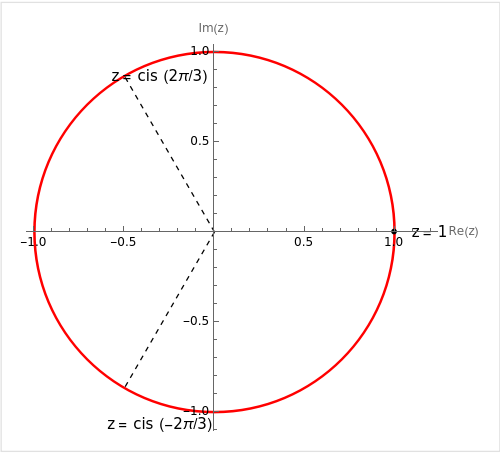
\includegraphics[width = 0.5\textwidth]{rootdemoivre.png}
    \caption{Solutions for $z^3=1$}
\end{figure}
The solutions are shown to lie on the unit circle at intervals of \( \frac{2\pi}{3} \) around the circle.
We find that the number of roots, of course, follows that the number of roots equal to the order of expression.

To generalize, we can see that there are exactly $m$ distinct $mth$ roots of unity, denoted
by
 \begin{equation}
    \boxed{1^{1/m}=e^{i2k\pi/m}=\cos\frac{2k\pi}m+i\sin\frac{2k\pi}m\quad(k=0,1,2, \ldots, m-1).}
 \end{equation}

\begin{theorem}[Solution of \( z^n = a \)] 

    For \( n \in \mathbb{N} \) and \( a \in \mathbb{C} \), the solutions of the equation \( z^n = a \) are called the \textit{n}th roots of \( a \).
\begin{itemize}[leftmargin=*]
    \item The solutions of \( z^n = a \) lie on a circle with center the origin and radius \( |a|^{1/n} \).
    \item There are \( n \) solutions and they are equally spaced around the circle at intervals of \( \frac{2\pi}{n} \). This observation can be used to find all solutions if one is known.
\end{itemize}
\end{theorem}   
More generally, consider any natural number \( n \geq 2 \). Using De Moivre's theorem, we can show that the \( n \)th roots of unity are
\[
1, \, \text{cis}\left(\frac{2\pi}{n}\right), \, \text{cis}\left(\frac{4\pi}{n}\right), \, \ldots, \, \text{cis}\left(\frac{2(n-1)\pi}{n}\right)
\]
So the \( n \)th roots of unity form a geometric sequence with common ratio \( \omega = \text{cis}\left(\frac{2\pi}{n}\right) \).
We can list the terms of this sequence as \( 1, \omega, \omega^2, \ldots, \omega^{n-1} \). The sum of the terms is
\[
1 + \omega + \omega^2 + \ldots + \omega^{n-1} = \frac{\omega^n - 1}{\omega - 1}
\]
since \( \omega^n = 1 \).
\begin{proof}
    The \( n \)th roots of unity are solutions to the equation \( z^n = 1 \). By expressing 1 in polar form as \( 1 \text{cis} 0 \), and applying De Moivre's theorem, \( (r \text{cis} \theta)^n = r^n \text{cis} (n\theta) \), we find that for \( z^n = 1 \), we must have \( z = \text{cis} \left(\frac{2k\pi}{n}\right) \), where \( k \) is an integer from \( 0 \) to \( n-1 \).

These solutions can be written as a sequence where each term after the first is obtained by multiplying the previous term by \( \text{cis} \left(\frac{2\pi}{n}\right) \), making it a geometric sequence with a common ratio of \( \omega = \text{cis} \left(\frac{2\pi}{n}\right) \).

The sum of a geometric sequence with \( n \) terms and a common ratio \( r \neq 1 \) is given by \( S_n = a_1 \frac{1-r^n}{1-r} \). For our sequence, \( a_1 = 1 \) and \( r = \omega \), so the sum is \( S_n = \frac{1-\omega^n}{1-\omega} \). Since \( \omega^n = \text{cis} (2\pi) = 1 \), the numerator becomes \( 1-1 = 0 \), hence the sum \( S_n \) is zero.
\end{proof}

To obtain the \( m \)th roots of an \textit{arbitrary} (nonzero) complex number \( z = re^{i\theta} \), we generalize the idea and, reasoning similarly, conclude that the \( m \) distinct \( m \)th roots of \( z \) are given by
\begin{equation}\label{mthroot}
    \boxed{z^{1/m} = \sqrt[m]{|z|}e^{i(\theta+2k\pi)/m} \quad (k = 0, 1, 2, \ldots, m - 1)}
\end{equation}

Equivalently, we can form these roots by taking any single one such as given in (3) and multiplying by the \( m \)th roots of unity.

\begin{example}
    Find all the cube roots of \( \sqrt{2} + i\sqrt{2} \).
\end{example}
\textbf{Solution:}
The polar form for \( \sqrt{2} + i\sqrt{2} \) is
\[
\sqrt{2} + i\sqrt{2} = 2e^{i\pi/4}.
\]
Putting \( |z| = 2 \), \( \theta = \pi/4 \), and \( m = 3 \) into Eq. \ref{mthroot}, we obtain
\[
(\sqrt{2} + i\sqrt{2})^{1/3} = \sqrt[3]{2}e^{i(\pi/12+2k\pi/3)} \quad (k = 0, 1, 2).
\]
Therefore, the three cube roots of \( \sqrt{2} + i\sqrt{2} \) are \( \sqrt[3]{2}(cos \pi/12 + i \sin \pi/12) \), \( \sqrt[3]{2}(cos 3\pi/4 + i \sin 3\pi/4) \), and \( \sqrt[3]{2}(cos 17\pi/12 + i \sin 17\pi/12) \).
\subsection{Exercises}

\begin{exercise}
    Let \( P(z) = 2z^3 + 9z^2 + 14z + 5 \).

\begin{itemize}
    \item[\textbf{a.}] Use the factor theorem to show that \( z + 2 - i \) is a linear factor of \( P(z) \).
    \item[\textbf{b.}] Write down another complex linear factor of \( P(z) \).
    \item[\textbf{c.}] Hence find all the linear factors of \( P(z) \) over \( \mathbb{C} \).
\end{itemize}
\end{exercise}
\textbf{Solution}

\textbf{a.} By the factor theorem, if \( z + 2 - i \) is a factor of \( P(z) \), then \( P(-2 + i) = 0 \). Calculating this we get:
\begin{align*}
P(-2 + i) &= 2(-2 + i)^3 + 9(-2 + i)^2 + 14(-2 + i) + 5 \\
&= 2(-8 - 12i + 6i^2) + 9(4 - 8i + 2i^2) + 14(-2 + i) + 5 \\
&= 2(-8 - 12i - 6) + 9(4 - 8i - 2) + (-28 + 14i) + 5 \\
&= -28 - 24i - 12 + 36 - 72i - 18 - 28 + 14i + 5 \\
&= 0.
\end{align*}
Thus, \( z + 2 - i \) is a linear factor of \( P(z) \).

\textbf{b.} By the conjugate root theorem, if \( z + 2 - i \) is a root, then its conjugate \( z + 2 + i \) is also a root.

\textbf{c.} Having found two complex roots, we can divide \( P(z) \) by the product of the corresponding factors to find the remaining factor. Let's perform the division (this is a mock example; the actual division should be computed):

% Example of polynomial division (mock)
\begin{align*}
P(z) &= (z + 2 - i)(z + 2 + i)(z - \alpha) \\
\end{align*}

After performing the division, we find that the remaining factor is \( z - \frac{1}{2} \). Thus, the linear factors of \( P(z) \) are:

\[
P(z) = (z + 2 - i)(z + 2 + i)\left(z - \frac{1}{2}\right)
\]

\begin{exercise}
    For a cubic polynomial \(P(x)\) with real coefficients, it is given that \(P(2 + i) = 0\), \(P(1) = 0\) and \(P(0) = 10\). Express \(P(x)\) in the form \(P(x) = ax^3 + bx^2 + cx + d\) and solve the equation \(P(x) = 0\).
\end{exercise}
\textbf{solution:}

Given that \(P(x)\) is a cubic polynomial with real coefficients and \(P(2 + i) = 0\), we know that its conjugate \(P(2 - i) = 0\) as well, due to the complex conjugate root theorem. Moreover, since \(P(1) = 0\), we can write \(P(x)\) as:

\[ P(x) = a(x - (2 + i))(x - (2 - i))(x - 1) \]

Expanding this and simplifying, we get:

\[ P(x) = a((x - 2)^2 + 1)(x - 1) \]

Since \(P(0) = 10\), we can find \(a\) by substituting \(x = 0\):

\[ 10 = a((0 - 2)^2 + 1)(0 - 1) \]
\[ 10 = a(4 + 1)(-1) \]
\[ 10 = -5a \]
\[ a = -2 \]

Thus, the polynomial is:

\[ P(x) = -2((x - 2)^2 + 1)(x - 1) \]
\[ P(x) = -2(x^2 - 4x + 4 + 1)(x - 1) \]
\[ P(x) = -2(x^2 - 4x + 5)(x - 1) \]
\[ P(x) = -2(x^3 - x^2 - 4x^2 + 4x + 5x - 5) \]
\[ P(x) = -2x^3 + 10x^2 - 18x + 10 \]

To solve for \(P(x) = 0\), we now have the equation:

\[ -2x^3 + 10x^2 - 18x + 10 = 0 \]

Since $P(2+i) = 0$, by conjugate root theorem, $p(2-i) = 0$, and we also have $p(1) = 0$.
The order of this expression is 3, by the fundamental algebra theorem, we have found all solutions.

\begin{exercise}
    If \( z = 1 + i \) is a zero of the polynomial \( z^3 + az^2 + bz + 10 - 6i \), find the constants \( a \) and \( b \), given that they are real.
\end{exercise}
\textbf{solution:}

Since \( z = 1 + i \) is a zero, by the Complex Conjugate Root Theorem, \( z = 1 - i \) is also a zero. Substituting \( z = 1 + i \) into the polynomial gives:

\begin{align*}
(1 + i)^3 + a(1 + i)^2 + b(1 + i) + 10 - 6i &= 0 \\
(1 + 3i - 3 - i) + a(1 + 2i - 1) + b + 10 - 6i &= 0 \\
(-2 + 2i) + a(2i) + b + 10 - 6i &= 0 \\
(-2 + (2a - 6)i) + b + 10 &= 0
\end{align*}

For the polynomial to be zero, both the real and imaginary parts must be zero. Therefore, we have two equations:

\begin{align*}
-2 + b + 10 &= 0 \quad \text{(Real part)} \\
2a - 6 &= 0 \quad \text{(Imaginary part)}
\end{align*}

Solving these equations gives us \( a \) and \( b \):

\begin{align*}
b &= -8 \\
a &= 3
\end{align*}

Thus, the constants are \( a = 3 \) and \( b = -8 \).

\begin{exercise}
    Let \( n \) be a positive integer. Prove that \[ \text{arg}(z^n) = n \text{Arg}(z) + 2k\pi, \quad k = 0, \pm1, \pm2, \ldots, \]
    \textbf{for} \( z \neq 0 \)
\end{exercise}
\begin{proof}
    Let's take \( z \in \mathbb{C} \). We can write \( z \) in its polar form as
\[ z = |z|(\cos \theta + i \sin \theta) \]

By definition of arg\( z \) and Arg\( z \) we have: \( \text{arg}(z) = \theta + 2k\pi, k \in \mathbb{Z}, \theta \in [-\pi, \pi] \) and \( \text{Arg}(z) = \text{arg}_{-}(z) = \theta, \theta \in [-\pi, \pi] \).

Now if we take the polar form of \( z^n \), where \( n \in \mathbb{N}, n \neq 0 \), we have
\[ z^n = |z|^n(\cos(n\theta) + i \sin(n\theta)) \]

\[ \Rightarrow \text{arg}(z^n) = n\theta + 2k\pi \]
\[ = n\text{Arg}(z) + 2k\pi, \quad k \in \mathbb{Z} \]

This concludes the proof.
\end{proof}

\begin{exercise}
    Find all the values of the following.
    \begin{enumerate}
        \item[(a)] \( (-16)^{1/4} \)
        \item[(b)] \( 1^{1/5} \)
        \item[(c)] \( i^{1/4} \)
        \item[(d)] \( (1 - \sqrt{3}i)^{1/3} \)
        \item[(e)] \( (i - 1)^{1/2} \)
        \item[(f)] \( \left(\frac{2i}{1+i}\right)^{1/6} \)
    \end{enumerate}
\end{exercise}



\begin{exercise}
    Find all four roots of the equation \( z^4 + 1 = 0 \) and use them to deduce the factorization \( z^4 + 1 = (z^2 - \sqrt{2}z + 1)(z^2 + \sqrt{2}z + 1) \).
\end{exercise}
\textbf{Solution:}

First, we solve the equation:
\begin{align*}
z^4 + 1 &= 0 \\
z^4 &= -1 \\
z &= \sqrt[4]{-1}
\end{align*}

Since \( -1 = \cos \pi + i \sin \pi \), we can find the roots using De Moivre's theorem:
\[ z = \sqrt[4]{\cos \pi + i \sin \pi} = \sqrt[4]{1}(\cos (\pi + 2k\pi)/4 + i \sin (\pi + 2k\pi)/4), \quad k = 0,1,2,3 \]

Thus, the roots are:
\begin{align*}
z_0 &= \cos \frac{\pi}{4} + i \sin \frac{\pi}{4} = \frac{1}{\sqrt{2}} + i \frac{1}{\sqrt{2}} \\
z_1 &= \cos \frac{3\pi}{4} + i \sin \frac{3\pi}{4} = -\frac{1}{\sqrt{2}} + i \frac{1}{\sqrt{2}} \\
z_2 &= \cos \frac{5\pi}{4} + i \sin \frac{5\pi}{4} = -\frac{1}{\sqrt{2}} - i \frac{1}{\sqrt{2}} \\
z_3 &= \cos \frac{7\pi}{4} + i \sin \frac{7\pi}{4} = \frac{1}{\sqrt{2}} - i \frac{1}{\sqrt{2}}
\end{align*}

To show the factorization, we pair the roots:
\begin{align*}
z^4 + 1 &= (z - z_0)(z - z_1)(z - z_2)(z - z_3) \\
&= \left(z - \frac{1}{\sqrt{2}} - i \frac{1}{\sqrt{2}}\right)\left(z + \frac{1}{\sqrt{2}} - i \frac{1}{\sqrt{2}}\right) \\
&\quad \times \left(z + \frac{1}{\sqrt{2}} + i \frac{1}{\sqrt{2}}\right)\left(z - \frac{1}{\sqrt{2}} + i \frac{1}{\sqrt{2}}\right) \\
&= \left(z^2 - \sqrt{2}z + 1\right)\left(z^2 + \sqrt{2}z + 1\right)
\end{align*}

And we have shown the factorization.

\begin{exercise}
    Let \( \alpha \) and \( \beta \) be the mth and nth roots of unity, respectively. We want to show that the product \( \alpha\beta \) is a kth root of unity for some integer \( k \).
\end{exercise}
\textbf{Solution:}

Let's consider \( \alpha \) as the m-th root of unity and \( \beta \) the n-th root of unity. Then we have
\[ \alpha^m = 1 \]
\[ \beta^n = 1 \]

Let's show that \( \alpha\beta \) is a root of unity. If \( \alpha\beta \) is a root of unity then there exists some \( l \in \mathbb{N} \) such that \( (\alpha\beta)^l = 1 \).

For \( l = mn \) (since \( m \) and \( n \) are relatively prime), we have
\[ (\alpha\beta)^l = (\alpha\beta)^{mn} \]
\[ = \alpha^{mn}\beta^{mn} \]
\[ = (\alpha^m)^n(\beta^n)^m \]
\[ = 1^n1^m \]
\[ = 1 \]

Thus, \( \alpha\beta \) is indeed a root of unity, specifically an \( mn \)-th root of unity.

\begin{exercise}
    Let \( m \) and \( n \) be positive integers that have no common factor. Prove that the set of numbers \( (z^{1/n})^m \) is the same as the set of numbers \( (z^m)^{1/n} \). We denote this common set of numbers by \( z^{m/n} \). Show that
\[ z^{m/n} = \sqrt[n]{|z|^m} \left[ \cos \left( \frac{m}{n} (\theta + 2k\pi) \right) + i \sin \left( \frac{m}{n} (\theta + 2k\pi) \right) \right] \]
for \( k = 0, 1, \ldots, n - 1 \).
\end{exercise}
\begin{proof}
    Let's take \( m, n \in \mathbb{N} \) so that they are relatively prime and \( z \in \mathbb{C} \) so that \( \text{Arg}(z) = \theta \). We have:
\begin{align*}
(z^{1/n})^m &= (\sqrt[n]{z})^m = \left( \sqrt[n]{|z|e^{i\theta}} \right)^m \\
&= \left( \sqrt[n]{|z|}e^{i\theta/n} \right)^m \\
&= |z|^{m/n} e^{im\theta/n}
\end{align*}

Now as \( m \) and \( n \) are relatively prime we have
\[ \frac{2k\pi}{n} \frac{m}{n} \quad k = 0, \ldots, n - 1 \]
from where
\begin{align*}
|z|^{m/n} e^{im(\theta + 2k\pi)/n} &= |z|^{m/n} e^{im\theta/n + im2k\pi/n} \\
&= (|z|^m)^{1/n} (e^{im\theta})^{1/n} \\
&= ((|z|^m e^{im\theta})^{1/n} \\
&= (z^m)^{1/n}
\end{align*}

To show the expression we take the previous result and expand it:
\begin{align*}
z^{m/n} &= |z|^{m/n} e^{im\theta/n} \\
&= \sqrt[n]{|z|^m} \left[ \cos \left( \frac{m\theta}{n} + \frac{2km\pi}{n} \right) + i \sin \left( \frac{m\theta}{n} + \frac{2km\pi}{n} \right) \right] \\
&= \sqrt[n]{|z|^m} \left[ \cos \left( \frac{m}{n} (\theta + 2k\pi) \right) + i \sin \left( \frac{m}{n} (\theta + 2k\pi) \right) \right]
\end{align*}
\end{proof}


\begin{exercise}
    Use the conclusion in last problem to evaluate $(i-i)^\frac{3}{2}$.
\end{exercise}
\textbf{Solution:}
It has been shown that
\begin{equation}
    \boxed{ z^{m/n} = \sqrt[n]{|z|^m}\left[\cos\left(\frac{m}{n}(\theta + 2k\pi)\right) + i\sin\left(\frac{m}{n}(\theta + 2k\pi)\right)\right]}
\end{equation}
We have:
\[ z = (1 - i)^{3/2} \Rightarrow m = 3, n = 2 \]
\[ |z| = \sqrt{1^2 + (-1)^2} = \sqrt{2} \]
\[ \theta = \text{Arg} z = 2\pi - \cot^{-1}\left(\frac{-1}{1}\right) = \frac{7\pi}{4} \]

When we put everything in the formula we get
\[ z = \sqrt[2]{\sqrt{2}^3}\left[\cos\left(\frac{3}{2}\left(\frac{7\pi}{4} + 2k\pi\right)\right) + i\sin\left(\frac{3}{2}\left(\frac{7\pi}{4} + 2k\pi\right)\right)\right], k = 0, 1 \]
\[ z = \sqrt[2]{2^{3/2}}\left[\cos\left(\frac{21\pi}{8} + \frac{3k\pi}{2}\right) + i\sin\left(\frac{21\pi}{8} + \frac{3k\pi}{2}\right)\right], k = 0, 1 \]
\[ z_0 = 2^{3/4}\left[\cos\left(\frac{21\pi}{8}\right) + i\sin\left(\frac{21\pi}{8}\right)\right] \]
\[ z_1 = 2^{3/4}\left[\cos\left(\frac{21\pi}{8} + \frac{3\pi}{2}\right) + i\sin\left(\frac{21\pi}{8} + \frac{3\pi}{2}\right)\right] \]
%------------------------------------------------




\part{Further Discrete Mathematics and Theories}
\chapterimage{orange2.jpg}
\chapterspaceabove{6.75cm} 
\chapterspacebelow{7.25cm} 
\chapter{Boolean Algebra}
    In the first chapter of this book, we discussed the very basic of mathematics, 
    proof and propositions. This chapter aims to excavate mathematical logics in 
    further details. With Boolean Algebra, we can explain more thoroughly on
    the mechanism of logics and mathematical proof, and on top of that, we can 
    figure out how computer functions, as well as how integrated circuits are 
    constructed.
    \section{Boolean Expression and Truth Table}
        We call Boolean Algebra "Algebra" of course, because it possesses property of Algebra.
        We will start with basic algebra operation and thus, proceed to get the rule of 
        Boolean operation, which we call the "Truth Table".
    \subsection{Property of Algebra Operation}
        For normal algebra operation of numbers, we have the following general law
        by representing the number in $x$, $y$, and $z$.
        \begin{table}[ht]
            \label{algelaw}
            \centering
            \caption{Common Algebraic Laws}
            \begin{tabular}{lll}
            \toprule
            \textbf{Law} & \textbf{Addition Expression} & \textbf{Multiplication Expression} \\
            \midrule
            Identity & \( x + 0 = x \) & \( x \cdot 1 = x \) \\
            Property of Zero & & \( x \cdot 0 = 0 \) \\
            Inverse & \( x + (-x) = 0 \) & \( x \cdot x^{-1} = 1 \), for \( x \neq 0 \) \\
            Commutative & \( x + y = y + x \) & \( x \cdot y = y \cdot x \) \\
            Associative & \( (x + y) + z = x + (y + z) \) & \( (x \cdot y) \cdot z = x \cdot (y \cdot z) \) \\
            Distributive & &\( x \cdot (y + z) = x \cdot y + x \cdot z \) \\
            \bottomrule
            \end{tabular}
        \end{table}
        In this case, we call $x$, $y$, and $z$ variables as in programming. for 
        all possible values of these variables, these laws hold.
        Why these laws are important is that all algebra expressions is derived
        from these laws, which means we can prove any equality that is correct.
        We take $-1 \time -1$ as an example. One may say without a second thought that
        the answer is 1. But why? Can we prove it? Now we try to prove it using the
        common algebraic laws.
        \begin{example}
            Prove that $(-1)\times (-1) = 1$
        \end{example}
        \begin{proof}
            \begin{align*}
                 & ( -1) \times ( -1)\\
                = & (( -1) \times ( -1)) +0\ ( Addition\ Identity\ )\\
                = & (( -1) \times ( -1)) +\ (( -1) +1) \ ( Addition\ Inverse)\\
                = & ((( -1) \times ( -1) +( -1)) +1\ ( Associative\ Law\ of\ Addition)\\
                = & ((( -1) \times ( -1) +(( -1) \times 1)) +1\ ( Multiplication\ Identity)\\
                = & (( -1) \times (( -1) +1)) +1\ ( Distributive\ Law)\\
                = & (( -1) \times 0) \ +\ 1\ ( Addition\ Inverse)\\
                = & 0+1\ ( Multiplication\ Property\ of\ Zero)\\
                = & 1+0\ (Commutative\ Law\ of\ Addition)\\
                = & 1\ ( Addition\ Identity)
            \end{align*}
            \begin{remark}
                Some people may not understand why we have to write $0+1$ into $1+0$. This is because
                Addition Identity is only defined in the table as $x+0=x$, so we need to apply Commutative
                law of addition to fit it into the known conclusion.
            \end{remark}
        \end{proof}

        After seeing this, you may think, do we really have to know this to make sure that $-1\times-1=1$?
        Of course not, but keep in mind that \textbf{Every mathematical conclusion cannot be simply referred as
        rules such as "a negative times negative give you a positive number", but by meticulous, reasonable, and 
        replicable proof.}

    \subsection{Boolean Expression and Truth Table}
        Hold on a second, isn't this chapter on Boolean Algebra? Why we still need to go over these
        old knowledge from primary school? Well, this is because we will prove Boolean expression in the
        same way. Before that, we introduce Boolean value and operations. 
        % Definition of Boolean Values
        \begin{definition}[Boolean Values]
        In mathematics and computer science, a Boolean value is defined as an element of the Boolean domain \(B\), which can be mathematically represented as:
        \[
        \B = \{0, 1\}
        \]
        where:
        \begin{itemize}
            \item \(0\) typically represents \textit{false}
            \item \(1\) typically represents \textit{true}
        \end{itemize}
        \end{definition}
        Some may be confused by true and false here. Just recall what we have done to propositions in
        the first chapter in this book. When a statement holds for given condition, we take it as
        correct, while incorrect when it does not hold. Boolean value is the basis of Boolean Expression,
        and \textbf{all valid boolean expression could be reduced or simplified to a Boolean value}.
        % Boolean Operations
        \begin{definition}[Boolean Operations]
        Boolean algebra involves operations such as AND, OR, NOT, XOR, which operate on these Boolean values. These operations are defined as follows:
        \begin{itemize}
            \item \textbf{AND} (\(\land\)): An operation on two Boolean values that returns \textit{true} if both operands are \textit{true}, otherwise returns \textit{false}.
            \item \textbf{OR} (\(\lor\)): An operation on two Boolean values that returns \textit{true} if at least one of the operands is \textit{true}, otherwise returns \textit{false}.
            \item \textbf{NOT} (\(\lnot\)): A unary operation that returns \textit{true} if the operand is \textit{false} and vice versa.
            \item \textbf{XOR} (\(\oplus\)): An operation on two Boolean values that returns \textit{true} if the operands are different, otherwise returns \textit{false}.
        \end{itemize}
        \begin{remark}
            There are more Boolean operators to be discussed later.
        \end{remark}
        \end{definition}
        In computer science, Boolean values are fundamental in conditional statements and loops, where they determine the flow of control in algorithms and programs. They are also essential in the design of electronic circuits and digital computing.
        The following table shows the truth table of these basic Boolean operations. the first column
        shows the combination of inputs for the specific operator, and the second column shows the
        result of operation.
        \begin{table}[ht] \label{truthtab}
            \centering % This centers the entire table construct
            
            \noindent
            \begin{tabular}{c|c}
            \textbf{A} & $\neg \textbf{A}$ \\
            \hline
            F & T \\
            T & F \\
            \end{tabular}
            \quad % Reduce the space between tables
            \begin{tabular}{cc|c}
            \textbf{A} & \textbf{B} & $\textbf{A} \land \textbf{B}$ \\
            \hline
            F & F & F \\
            F & T & F \\
            T & F & F \\
            T & T & T \\
            \end{tabular}
            
            \vspace{2mm} % Reduce the vertical space between the rows of tables
            
            \noindent
            \begin{tabular}{cc|c}
            \textbf{A} & \textbf{B} & $\textbf{A} \lor \textbf{B}$ \\
            \hline
            F & F & F \\
            F & T & T \\
            T & F & T \\
            T & T & T \\
            \end{tabular}
            \quad % Reduce the space between tables
            \begin{tabular}{cc|c}
            \textbf{A} & \textbf{B} & $\textbf{A} \oplus \textbf{B}$ \\
            \hline
            F & F & F \\
            F & T & T \\
            T & F & T \\
            T & T & F \\
            \end{tabular}
            
            \caption{Common Boolean Operators Truth Tables}
        \end{table}

        It's noticeable that different Boolean operators may differ in the number of input. $\lnot$ operator
        takes only one Boolean variable (input) to get an output by negating the input, however the rest 
        take two inputs and produce one output. 
        
        At the beginning of the section, we have defined Boolean
        space $B=\{0,1\}$, but why George Boole(The British mathematician who initiate this idea) define 
        Boolean value with a set containing only zero and one? This is actually because, \textbf{The foundation
        of Boolean Algebra is set upon operations involving 0 and 1}. To explicit, I need to clarify that
        among the four operators introduced above, $\lnot$, $\land$, and $\lor$ are the very basic of all
        Boolean expressions, which means other Boolean operators could be written in an equivalent form with
        these basic operators. For example, we can write XOR($\oplus$) in the other three operators:
        \begin{equation}
            \label{xor}
            A \oplus B= (A \land \lnot B) \lor(\lnot A \land B)
        \end{equation}
        It doesn't really matter if you find the RHS strange,as all we need now is just know the fact 
        that we can write it in this form. We will discuss the expression in details in the next section.
        Now let's refocus on Boolean space \{0,1\}. We all know that there are four basic operations in 
        algebra which are addition, subtraction, multiplication, and division. But generally, we say there 
        are only two basic operations in algebra, which are $+$ and $\times$, as subtraction and division are
        just inverse operation of addition and multiplication. Let's look in to the table of addition and 
        multiplication of 0 and 1 listed below.
        \begin{table}[ht]
            \centering % This centers the entire table construct
            \noindent
            \begin{tabular}{cc|c}
                A & B & $A \times B$ \\
                \hline
                0 & 0 & 0 \\
                0 & 1 & 0 \\
                1 & 0 & 0 \\
                1 & 1 & 1 \\
            \end{tabular}
            \quad
            \begin{tabular}{cc|c}
                A & B & $A + B$ \\
                \hline
                0 & 0 & 0 \\
                0 & 1 & 1 \\
                1 & 0 & 1 \\
                1 & 1 & 1 \\     
            \end{tabular}
        \caption{Addition and Multiplication Rule of 0 and 1}
        \end{table}

        Now you may have realized that this is exactly the truth table for $\land$ and $\lor$, you may
        check table \ref{truthtab}.
    
        \subsection{Boolean Identities}
        Now recall that $A \oplus B= (A \land \lnot B) \lor(\lnot A \land B)$. In this
        expression, we cannot get a direct answer from the RHS by using the truth table of $\lor$. So,
        we need to try harder to get the truth table for the expression as shown in the table below.
        \begin{table}[ht]
            \centering
            \caption{Truth table for \((A \land \neg B) \lor (\neg A \land B)\)}
            \begin{tabular}{cc|c|c|c|c|c}
            \hline
            \( A \) & \( B \) & \( \neg B \) & \( A \land \neg B \) & \( \neg A \) & \( \neg A \land B \) & \( (A \land \neg B) \lor (\neg A \land B) \) \\ \hline
            F & F & T & F & T & F & F \\
            F & T & F & F & T & T & T \\
            T & F & T & T & F & F & T \\
            T & T & F & F & F & F & F \\ \hline
            \end{tabular}
            
        \end{table}

        With this method, we can find truth table for more complex expressions, and some of them
        are categorized as \textbf{Basic Boolean Identities}. The LHS and RHS are could be proven qaual
        by listing truth table respectively.

        \begin{table}[H]
            \centering
            \caption{Basic Boolean Identities}
            \begin{tabular}{lll}
            \toprule
            \textbf{Identity} & \textbf{AND Form} & \textbf{OR Form} \\
            \midrule
            Idempotent Law & \( x \cdot x = x \) & \( x + x = x \) \\
            Identity Law & \( x \cdot 1 = x \) & \( x + 0 = x \) \\
            Domination Law & \( x \cdot 0 = 0 \) & \( x + 1 = 1 \) \\
            Complement Law & \( x \cdot \lnot x = 0 \) & \( x + \lnot x = 1 \) \\
            Double Negation Law & \( \lnot(\lnot x) = x \) & \( \lnot(\lnot x) = x \)\\
            Commutative Law & \( x \cdot y = y \cdot x \) & \( x + y = y + x \) \\
            Associative Law & \( x \cdot (y \cdot z) = (x \cdot y) \cdot z \) & \( x + (y + z) = (x + y) + z \) \\
            Distributive Law & \( x \cdot (y + z) = (x \cdot y) + (x \cdot z) \) & \( x + (y \cdot z) = (x + y) \cdot (x + z) \) \\
            De Morgan's Law & \( \lnot(x + y) = \lnot x \cdot \lnot y \) & \( \lnot(x \cdot y) = \lnot x + \lnot y \) \\
            Absorption Law & \( x \cdot (x + y) = x \) & \( x + (x \cdot y) = x \) \\
            \bottomrule
            \end{tabular}
        \end{table}
        \begin{remark}
            If you are confused by the algebra form of Boolean identities, just take $x$, $y$, $z$ as
            $A$, $B$, and $C$; take 0/1 as F/T; take + as $\lor$, and $\times$ as $\land$.
        \end{remark}
        It is quite important to be familiar with these rules, as they are just as essential as
        the normal algebra laws we've learned before, since we may simplify complex Boolean expressions
        using these rules. Also, the proof of some of these identities using truth table will be 
        added to the problem set for this section. If you remain any doubt or confusion about any laws
        given, just try to get the truth table for the LHS and RHS of the identity, simple as that.

        This is actually not yet a complete table of Boolean Identities, two laws are still missing
        from the table, because they are relevant to secondary operator, one of which is already mentioned($\oplus$).

        With these basic Boolean laws, we can derive more interesting and useful theorems. A commonly used theorem when simplifying
        Boolean expression is concensus (or also called redundancy) theorem.
        \begin{theorem}[Concensus Theorem]
            The Consensus Theorem helps simplifying Boolean expressions by eliminating a redundant term, and like other laws, it has both
            OR and AND form. 
            It states that for any Boolean variables $x$, $y$, and $z$:
            \begin{equation*}
                xy\lor\bar{x}z\lor yz=xy\lor\bar{x}z
            \end{equation*}
            Which is equivalent to
            \begin{equation*}
                (x\lor y)(\bar{x}\lor z)(y\lor z)=(x\lor y)(\bar{x}\lor z)
            \end{equation*}
        \end{theorem}
        \begin{proof}
            $$\begin{aligned}
                xy\lor\bar{x}z\lor yz& =xy\lor\bar{x}z\lor(x\lor\bar{x})yz  \\
                &=xy\lor\bar{x}z\lor xyz\lor\bar{x}yz \\
                &=(xy\lor xyz)\lor(\bar{x}z\lor\bar{x}yz) \\
                &=xy(1\lor z)\lor\bar{x}z(1\lor y) \\
                &=xy\lor\bar{x}z
                \end{aligned}$$
            Or in another notation.
            $$\begin{aligned}
                xy + \overline{x}z + yz &= xy + \overline{x}z + (x + \overline{x})yz \\
                &= xy + \overline{x}z + xyz + \overline{x}yz \\
                &= (xy + xyz) + (\overline{x}z + \overline{x}yz) \\
                &= xy(1 + z) + \overline{x}z(1 + y) \\
                &= xy + \overline{x}z
                \end{aligned}$$
        \end{proof}


        \subsubsection*{Secondary Boolean Operators}
        \begin{definition}[Secondary Boolean Operators]
            Secondary operators are derived from basic operators:
            \begin{itemize}
                \item Material conditional: \( x \rightarrow y = \lnot x \lor y \)
                \item Material biconditional: \( x \leftrightarrow y = (x \land y) \lor (\lnot x \land \lnot y) \)
                \item Exclusive OR (XOR): \( x \oplus y = \lnot(x \leftrightarrow y) = (x \lor y) \land (\lnot x \lor \lnot y) = (x \land \lnot y) \lor (\lnot x \land y) \)
                \end{itemize}
        \end{definition}

        Their truth tables for the secondary operation are below:
        \begin{table}[H]
        \centering
        \begin{tabular}{cc|c|c|c}
        \hline
        \( x \) & \( y \) & \( x \rightarrow y \) & \( x \leftrightarrow y \) & \( x \oplus y \) \\
        \hline
        0 & 0 & 1 & 1 & 0 \\
        1 & 0 & 0 & 0 & 1 \\
        0 & 1 & 1 & 0 & 1 \\
        1 & 1 & 1 & 1 & 0 \\
        \hline
        \end{tabular}
        \caption{Truth values of material conditional, biconditional, and XOR for all possible inputs.}
        \end{table}
        The $\rightarrow$ operation holds that $x \rightarrow x = 1$. This expression means
        that when $x=y$, then $x\rightarrow y$ must be true. The complete form of secondary operators
        and the implication identity will be the last Boolean identity to be covered in this chapter.
        \begin{enumerate}
            \item Material Conditional (\(\rightarrow\)):
            The material conditional \( x \rightarrow y \) is read as "if \( x \) then \( y \)" or "\( x \) implies \( y \)". It represents the logical implication. The truth value of \( x \rightarrow y \) is false only when \( x \) is true and \( y \) is false; in all other cases, it is true. This is a bit counter-intuitive when \( x \) is false because the implication will be true regardless of the value of \( y \). It can be expressed using basic operations as \( \lnot x \lor y \).
            
            \item Material Biconditional (\(\leftrightarrow\)):
            The material biconditional \( x \leftrightarrow y \), also known as logical equivalence, is the operation that is true when \( x \) and \( y \) have the same truth values, and false otherwise. It's often read as " \( x \) if and only if \( y \)". It can be formulated as \( (x \land y) \lor (\lnot x \land \lnot y) \), meaning both \( x \) and \( y \) are true, or both are false.
            
            \item Exclusive OR (XOR):
            The exclusive OR \( x \oplus y \) is true when \( x \) and \( y \) have different truth values — that is, one is true and the other is false. It differs from the regular OR operation in that \( x \oplus y \) is false when both \( x \) and \( y \) are true. It can be represented as \( (x \land \lnot y) \lor (\lnot x \land y) \).
        \end{enumerate}
        
        With these basic identities and operators, we can prove more interesting Boolean theorems.
        Below are more theorems to be proved as example. Maybe you are ready to draw a truth table to prove
        them. However, with these basic Boolean Laws, we actually don't have to do that, but prove it
        by using Algebra techniques.
        \begin{example}
            Prove the following identities using the table given earlier.
        \begin{table}[ht]
            \centering
            \begin{tabular}{ll}
            \toprule
            \textbf{Expression} & \textbf{Name} \\
            \midrule
            \( (x \rightarrow \text{False}) = (\lnot x) \) & $\lnot$ as \(\rightarrow\) \\
            \( (x \rightarrow y) = (\lnot y \rightarrow \lnot x) \) & contrapositive \\
            \( ((x \rightarrow y) \land (x \rightarrow z)) = (x \rightarrow (y \land z)) \) & implication \\
            \( ((x \rightarrow y) \land (\lnot x \rightarrow y)) = y \) & absurdity \\
            \( (x \rightarrow (\lnot x)) = (\lnot x) \) & contradiction \\
            \bottomrule
            \end{tabular}
        \end{table}
        \end{example}

        \begin{proof}
            To prove $\lnot$ as \(\rightarrow\), we just need to use the definition of $
            \rightarrow$.
            $$x\rightarrow\text{ False}= \lnot x \lor False = \lnot x + 0 = \lnot x \ \text{(OR Identity Law)}$$
            
            The contrapositive identity states that \( (x \rightarrow y) \) is logically equivalent to \( (\lnot y \rightarrow \lnot x) \).
            \begin{align*}
            x \rightarrow y &\equiv \lnot x \lor y \\
                &\equiv y \lor \lnot x\ \text{(Commutative Law)}\\
            &\equiv \lnot y \rightarrow \lnot x
            \end{align*}
            \begin{remark}
                This proof shows why proof by contrapositive (mentioned in chapter1) is correct.
            \end{remark}
            The implication identity can be proved by showing that \( (x \rightarrow y) \land (x \rightarrow z) \) is equivalent to \( x \rightarrow (y \land z) \).
            \begin{align*}
            (x \rightarrow y) \land (x \rightarrow z) &\equiv (\lnot x \lor y) \land (\lnot x \lor z) \\
            &\equiv \lnot x \lor (y \land z) \\
            &\equiv x \rightarrow (y \land z)
            \end{align*}

            The absurdity identity states that \( (x \rightarrow y) \land (\lnot x \rightarrow y) \) is equivalent to \( y \).
            \begin{align*}
            (x \rightarrow y) \land (\lnot x \rightarrow y) &\equiv (\lnot x \lor y) \land (x \lor y) \\
            &\equiv y \lor (x \land \lnot x) \\
            &\equiv y \lor \text{False} \\
            &\equiv y
            \end{align*}

            The contradiction identity states that \( x \rightarrow (\lnot x) \) is equivalent to \( \lnot x \).
            \begin{align*}
            x \rightarrow (\lnot x) &\equiv \lnot x \lor (\lnot x) \\
            &\equiv \lnot x
            \end{align*}
        \end{proof}
        \begin{remark}
            Some may feel confused by the notation of Boolean expression we use in this chapter.
            Sometimes we use logic notation, while sometimes use algebra operation. Both are ok,
            it's really up to your preference.
        \end{remark}
        When you look through the whole process, you'll find that we are actually doing the same
        thing as simplifying Boolean expressions, where all the laws could be used so that we don't
        need to draw truth table again and again.

        




        \subsection{Exercises}
        \begin{exercise}
            Use table \ref{algelaw} and $1+1=2$ to show that $(x+x)=(2\times x)$.
        \end{exercise}
        \begin{proof}
            \begin{align*}
                ( 2\times x) & =( 1+1) \times x\ ( by\ 1+1=2)\\
                & =\ 1\times x+1\times x\ ( Distributive\ Law)\\
                & =x+x\ ( Multiplication\ Identity)
            \end{align*}
        \end{proof}
        \begin{exercise}
            Show that $((-1)\times x)+x=0$ using the table.
        \end{exercise}
        \begin{proof}
            \begin{align*}
                (( -1) \times x) +x & =x( -1+1) \ ( Distributive\ Law)\\
                 & =\ x\times 0\ ( Addition\ Inverse)\\
                 & =0\ ( Multiplication\ Property\ of\ Zero)
            \end{align*}
        \end{proof}
        \begin{exercise}
            Show that $(x+(((-1)\times (x+y))+z)) + y =z$, you may use the conclusion of previous
            exercise.
        \end{exercise}
        \begin{proof} 
            To make it clear, we use square and curly bracket for different layers of parenthesis.
            \begin{align*}
                \  & \{x+[((-1) \times ( x+y)) +z]\} +y\\
                & =\{x+[(( -1) \times x) +(( -1) \times y)] +z\} +y\ ( Distributive\ Law\ )\\
                & =\{x+(( -1) \times x) +[(( -1) \times y) +z]\} +y\ ( Associative\ Law\ of\ Addition)\\
                & =\{(( -1) \times x) +x+\ [(( -1) \times y) +z]\} +y( Commutative\ Law\ of\ Addition)\\
                & =0+\{[(( -1) \times y) +z] +y\}\ ( Previous\ Conclusion)\\
                & =\{[(( -1) \times y) +z] +y\} +0\ ( Commutative\ Law\ of\ Addition)\\
                & =\{[(( -1) \times y) +z] +y\} \ ( Addition\ Identity)\\
                & =(( -1) \times y) +( z+y) \ ( Associative\ Law\ of\ Addition)\\
                & =( z+y) +(( -1) \times y) \ ( Commutative\ Law\ of\ Addition)\\
                & =z+[ y+(( -1) \times y)] \ ( Associative\ Law\ of\ Addition)\\
                & =z+[(( -1) \times y) +y] \ ( Commutative\ Law\ of\ Addition)\\
                & =z+0\ ( Previous\ Conclusion)\\
                & =z\ ( Addition\ Identity)
            \end{align*}
            
        \end{proof}
        
        \begin{exercise}
            Use truth table to show that De Morgan's Law is correct.
        \end{exercise}
        \begin{proof}
            De Morgan's First Law: \( \lnot (A \land B) = \lnot A \lor \lnot B \)
            
            \begin{tabular}{cc|c|c|c}
            \toprule
            \( A \) & \( B \) & \( A \land B \) & \( \lnot (A \land B) \) & \( \lnot A \lor \lnot B \) \\
            \midrule
            0 & 0 & 0 & 1 & 1 \\
            0 & 1 & 0 & 1 & 1 \\
            1 & 0 & 0 & 1 & 1 \\
            1 & 1 & 1 & 0 & 0 \\
            \bottomrule
            \end{tabular}

            \vspace{2em} 

            De Morgan's Second Law: \( \lnot (A \lor B) = \lnot A \land \lnot B \)

            \begin{tabular}{cc|c|c|c}
            \toprule
            \( A \) & \( B \) & \( A \lor B \) & \( \lnot (A \lor B) \) & \( \lnot A \land \lnot B \) \\
            \midrule
            0 & 0 & 0 & 1 & 1 \\
            0 & 1 & 1 & 0 & 0 \\
            1 & 0 & 1 & 0 & 0 \\
            1 & 1 & 1 & 0 & 0 \\
            \bottomrule
            \end{tabular}
        \end{proof}

        \begin{exercise}
            Use truth table to show that Absorption Law is correct.
        \end{exercise}
        \begin{proof}
            \begin{tabular}{cc|c|c}
                \hline
                \( x \) & \( y \) & $x \lor y$&\( x \land (x \lor y) \) \\
                \hline
                T & T & T & T \\
                T & F & T & T \\
                F & T & F & F \\
                F & F & F & F \\
                \hline
            \end{tabular}
            \quad
            \begin{tabular}{cc|c|c}
                \hline
                \( x \) & \( y \)&$x \land y$ & \( x \lor (x \land y) \) \\
                \hline
                T & T& T& T \\
                T & F& F& T \\
                F & T& F& F \\
                F & F& F& F \\
                \hline
            \end{tabular}
        \end{proof}

        \begin{exercise}
            Show the truth table of $\displaystyle x\lor (( \lnot y) \land ( \lnot z))$.
        \end{exercise}
        \textbf{Hint:} For Boolean expression of 3 variable, there will be more combinations.
        
        \textbf{Solution:}

        \begin{table}[ht]
            \centering
            \caption{Truth table for the expression \( x \lor ((\lnot y) \land (\lnot z)) \)}
            \begin{tabular}{ccc|c|c|c|c}
            \hline
            \( x \) & \( y \) & \( z \) & \( \lnot y \) & \( \lnot z \)& $(\lnot y) \land (\lnot z)$ & \( x \lor ((\lnot y) \land (\lnot z)) \) \\
            \hline
            0 & 0 & 0 & 1 & 1 &1& 1 \\
            0 & 0 & 1 & 1 & 0 &0& 0 \\
            0 & 1 & 0 & 0 & 1 &0& 0 \\
            0 & 1 & 1 & 0 & 0 &0& 0 \\
            1 & 0 & 0 & 1 & 1 &0& 1 \\
            1 & 0 & 1 & 1 & 0 &0& 1 \\
            1 & 1 & 0 & 0 & 1 &0& 1 \\
            1 & 1 & 1 & 0 & 0 &0& 1 \\
            \hline
            \end{tabular}
 
        \end{table}

        \begin{exercise}
            Given the expressions:
            \begin{align*}
            1. & \quad (x \rightarrow y) \land (\lnot x \rightarrow \lnot y) \\
            2. & \quad ((\lnot x) \lor y) \land (x \lor (\lnot y)) \\
            3. & \quad \lnot((x \land (\lnot y)) \lor ((\lnot x) \land y)) \\
            4. & \quad \lnot((x \lor y) \land (\lnot x \lor \lnot y)) \\
            \end{align*}
            Show that they are equivalent and find the common (simplified) form of the four expression
        \end{exercise}
        \begin{proof}
            \begin{align*}
                (x \rightarrow y) \land (\neg x \rightarrow \neg y) & \equiv (\neg x \lor y) \land (x \lor \neg y) && \text{(Implication equivalence)} \\
                & \equiv (x \lor \neg y) \land (\neg x \lor y) && \text{(Commutativity of OR)} \\
                & \equiv (x \lor \neg y) \land (y \lor \neg x) && \text{(Commutativity of AND)}
                \end{align*}

                \begin{align*}
                    ((\neg x) \lor y) \land (x \lor (\neg y)) & \equiv (y \lor \neg x) \land (x \lor \neg y) && \text{(Commutativity of OR)} \\
                    & \equiv (x \lor \neg y) \land (y \lor \neg x) && \text{(Commutativity of AND)}
                    \end{align*}
            
                    \begin{align*}
                        \neg((x \land (\neg y)) \lor ((\neg x) \land y)) & \equiv \neg(x \land (\neg y)) \land \neg((\neg x) \land y) && \text{(De Morgan's laws)} \\
                        & \equiv (\neg x \lor y) \land (x \lor \neg y) && \text{(De Morgan's laws)} \\
                        & \equiv (x \lor \neg y) \land (y \lor \neg x) && \text{(Commutativity of OR and AND)}
                        \end{align*}

                        \begin{align*}
                            \neg((x \lor y) \land (\neg x \lor \neg y)) & \equiv \neg(x \lor y) \lor \neg(\neg x \lor \neg y) && \text{(De Morgan's laws)} \\
                            & \equiv (\neg x \land \neg y) \lor (x \land y) && \text{(De Morgan's laws)} \\
                            & \equiv (x \land y) \lor (\neg x \land \neg y) && \text{(Commutativity of OR)} \\
                            & \equiv (x \lor \neg y) \land (y \lor \neg x) && \text{(Distribution)}
                            \end{align*}
                            

            These expressions could be simplified to $(\lnot y \lor x)\land(\lnot x\lor y)$, or
            $(y\rightarrow x)\land(x\rightarrow y)$, which can also be understood as $x$ and $y$
            cannot be true of false in the same time.
        \end{proof}

        \begin{exercise}
            Show that the concensus theorem's two forms are equivalent.
                $$xy\lor\bar{x}z\lor yz=xy\lor\bar{x}z$$
            and
                $$(x\lor y)(\bar{x}\lor z)(y\lor z)=(x\lor y)(\bar{x}\lor z)$$
            are equivalent.
        \end{exercise}
        \textbf{Solution:}
        We can simplify the product form to the standard form easily.
        \begin{align*}
            (x \lor y)(\overline{x} \lor z)(y \lor z) &= x\overline{x} \lor xz \lor y\overline{x} \lor yz \lor xy \lor xz \lor y^2 \lor yz \\
            &= 0 \lor xz \lor y\overline{x} \lor yz \lor xy \lor xz \lor y \lor yz \\
            &= xz \lor y\overline{x} \lor yz \lor xy \\
            &= xy \lor xz \lor y\overline{x}
        \end{align*}

    \section{Boolean Function}
    This section will bring you some further ideas of Boolean operation. Just like we can take a normal algebra
    expression, such as $2x+3$, as a function $f(x)=2x+3$; we can define \textbf{Boolean Function}
    with Boolean operation.
    \begin{definition}[Boolean Function]
    A Boolean function is a function that returns a Boolean value (true or false) for each possible combination of Boolean inputs. 
    $f: B^n \rightarrow B$ is a function from the set of  $n$-tuples of Boolean values to the set of Boolean values, where  $B = \{0, 1\}$.
    \end{definition} 
    For example, we can write the basic operations we just went over in Boolean Functions:
    \begin{enumerate}
        \item Algebraic notation:
        \begin{itemize}
            \item AND: $f(x, y) = x \cdot y$ or $f(x, y) = xy$
            \item OR: $f(x, y) = x + y$
            \item NOT: $f(x) = x'$ or $f(x) = \overline{x}$
        \end{itemize}
        
        \item Logical notation:
        \begin{itemize}
            \item AND: $f(x, y) = x \wedge y$
            \item OR: $f(x, y) = x \vee y$
            \item NOT: $f(x) = \neg x$
        \end{itemize}
    \end{enumerate}

    We have actually learned about this earlier in the chapter. Think about what we have done using truth tables. Just like what you have done at the beginning of 
    learning functions, you were making tables to show all results of each input with their output. For Preliminary functions, we always have 
    $f: R\rightarrow R$, which makes the mapping hard to make table, because there are infinite many real numbers. But things is much easier for Boolean function,
    because we have known in the definition that each function generate only one single output, and the most important part is that we always have limited inputs.
    Since $|B|=2$ for the Boolean Domain, so each input gives us 2 choices only, and therefore when we have $n$ inputs, we have $2^n$ cases only. $2^n$ seems huge,
    but in most cases we have less than 5 inputs in a Boolean function, so the size of the table is still manageable.

    \subsection{Representation of Boolean Function}
    In most cases, we construct a Boolean Function from a given truth table. All Boolean functions could be represented in both
    Disjunctive Normal Form (also known as sum of product;SOP form) and Conjunctive Normal Form (also known as Product of Sum;POS form).
    \begin{definition}[SOP Form]
        The Sum of Products (SOP) form, also known as the Disjunctive Normal Form (DNF), is a way to represent a Boolean function as a sum (logical OR) of product (logical AND) terms. Each product term consists of literals (variables or their complements) that correspond to the function's minterms, which are the input combinations that result in a function value of 1.
        The general form of an SOP expression is:
        \[f(x_1, x_2, \ldots, x_n) = \sum_{i=1}^{m} \prod_{j=1}^{n} x_j^{(i)},\]
        where $m$ is the number of minterms, $n$ is the number of variables, and $x_j^{(i)}$ is either $x_j$ or $x_j'$ (complement of $x_j$) depending on the value of $x_j$ in the $i$-th minterm.
    \end{definition}

    \begin{definition}[POS Form]
        The Product of Sums (POS) form, also known as the Conjunctive Normal Form (CNF), is a way to represent a Boolean function as a product (logical AND) of sum (logical OR) terms. Each sum term consists of literals (variables or their complements) that correspond to the function's maxterms, which are the input combinations that result in a function value of 0.
        The general form of a POS expression is:
        \[f(x_1, x_2, \ldots, x_n) = \prod_{i=1}^{M} \sum_{j=1}^{n} x_j^{(i)},\]
        where $M$ is the number of maxterms, $n$ is the number of variables, and $x_j^{(i)}$ is either $x_j$ or $x_j'$ (complement of $x_j$) depending on the value of $x_j$ in the $i$-th maxterm.
        \end{definition}
    \begin{remark}
        Minterms and maxterms are fundamental building blocks for representing Boolean functions, corresponding to the input combinations that result in function values of 1 and 0, respectively.
    \end{remark}

    But why we are so obsessed with whether the output for one single row is 1(T) or 0 (F)?
    This is because, when we are constructing a Boolean function, we are trying to make the mapping
    from $B^n$ to $B$, while $B = {0,1}$. Hence, we could conclude that the result of boolean function
    is actually binary, meaning only two cases for the output(we will talk about it later in the chapter).   
    So, we only need to figure out either of all the cases where the output is 0, or all the cases where the 
    output  is 1. This actually explains what are stated in the \textbf{Canonical Form Theorem}.
    \begin{theorem}[Canonical Form Theorem]
        Any Boolean function can be expressed in either of two canonical forms:
        \begin{enumerate}
        \item Sum of Products (SOP) form, also known as the Disjunctive Normal Form (DNF): Any Boolean function can be represented as a disjunction (OR) of one or more minterms, where a minterm is a product (AND) of literals corresponding to the rows in the truth table where the function value is 1.
        \item Product of Sums (POS) form, also known as the Conjunctive Normal Form (CNF): Any Boolean function can be represented as a conjunction (AND) of one or more maxterms, where a maxterm is a sum (OR) of literals corresponding to the rows in the truth table where the function value is 0.
        \end{enumerate}
        \end{theorem}
        
        \begin{proof}
        To prove the Canonical Form Theorem, we will consider an arbitrary Boolean function $f(x_1, x_2, \ldots, x_n)$ and show that it can be expressed in both SOP and POS forms.
        
        \textbf{Proof of SOP form (DNF):}
        \begin{enumerate}
        \item For each row in the truth table where the function value is 1, create a minterm by taking the conjunction (AND) of the literals corresponding to the input values in that row. If the input variable is 1, use the original variable; if the input variable is 0, use the complement of the variable.
        \item Take the disjunction (OR) of all the minterms obtained in step 1. This resulting expression is the SOP form of the Boolean function.
        \end{enumerate}
        
        Since every row where the function value is 1 is represented by a minterm, and the disjunction of these minterms covers all the cases where the function is 1, the resulting SOP form is equivalent to the original Boolean function.
        
        \textbf{Proof of POS form (CNF):}
        \begin{enumerate}
        \item For each row in the truth table where the function value is 0, create a maxterm by taking the disjunction (OR) of the literals corresponding to the input values in that row. If the input variable is 0, use the original variable; if the input variable is 1, use the complement of the variable.
        \item Take the conjunction (AND) of all the maxterms obtained in step 1. This resulting expression is the POS form of the Boolean function.
        \end{enumerate}
        
        Since every row where the function value is 0 is represented by a maxterm, and the conjunction of these maxterms covers all the cases where the function is 0, the resulting POS form is equivalent to the original Boolean function.
        
        Therefore, any Boolean function can be expressed in either SOP or POS form, proving the Canonical Form Theorem.
        \end{proof}
    \begin{example}
        Considering
        \begin{tabular}{|c|c|c|}
            \hline
            x & y & f(x, y) \\
            \hline
            0 & 0 & 1 \\
            \hline
            0 & 1 & 0 \\
            \hline
            1 & 0 & 0 \\
            \hline
            1 & 1 & 1 \\
            \hline
            \end{tabular}
            .If you are familiar with the Boolean operations, you may have realized this is actually a XNOR operation, which negates XOR.
            We will try to get the Algebra expression of this function in both POS and SOP.
             
    \end{example}
    \begin{solution}
                For the SOP form:
                \begin{itemize}
                    \item Function value is 1 for the corresponding input combinations.
                    \item Smallest terms: $m_0 = x'y'$, $m_3 = xy$.
                    \item SOP form of the Boolean function: $f(x, y) = m_0 + m_3 = x'y' + xy$.
                \end{itemize}
            
                For the POS form:
                \begin{itemize}
                    \item Function value is 0 for the corresponding input combinations.
                    \item Largest terms: $M_1 = x + y'$, $M_2 = x' + y$.
                    \item POS form of the Boolean function: $f(x, y) = M_1 \cdot M_2 = (x + y')(x' + y)$.
                \end{itemize}
                
             These two forms can be converted to each other based on the truth table of a Boolean function.
            \end{solution}

    This method also works for Boolean functions with more variables, and the only difference is that it may take a little more time.
    You may check more relevant problems in the exercises.
    
    \subsection{Properties of Boolean Function}
    In this part of the chapter, we will look into further details of Boolean Expression, specifically, Boolean Function. As an intro, we start with completeness
    and duality of Boolean Function. After this, we will introduce the Fundamental Theorem of Boolean Algebra, also known as Boole's expansion theorem (or Shannon expansion), 
    which in the foundation of logic circuit design and implementation.
    \begin{theorem}[Completeness of Boolean Function]
        A set of Boolean operators is said to be \textit{functionally complete} if every Boolean function can be expressed using only those operators. The following sets are known to be functionally complete:

        \begin{enumerate}
            \item The set \{AND, OR, NOT\}, also known as the standard or canonical basis.
            \item The set \{NAND\}, known as the NAND-only implementation.
            \item The set \{NOR\}, known as the NOR-only implementation.
        \end{enumerate}

        The completeness property is important in digital logic design, as it allows designers to create any desired Boolean function using a minimal set of logic gates.
    \end{theorem}

    \begin{remark}
        If you are getting confused by the word "Logic Gate", just take it as another way we call Boolean or Logic Operators. Logic gates are what electric engineers use
        to construct Boolean circuits, which is not discussed in details in this book, since we only discuss the mathematical aspect of this practice. You may refer
        to \href{https://www.wikiwand.com/en/Logic_gate}{this link}
        if you want to get more details. 
    \end{remark}
    To further illustrate, we could say that all Boolean Functions, or Boolean expressions can be expressed by either combinations of \{AND, OR, NOT\}, or NAND gates(s), or NOR gate(s).
    The first point is already quite clear, we have shown that all secondary operators can be written equivalently in basic operators, \{AND, OR, NOT\}. While NAND and NOR are general 
    logic gates that could construct any logic gates. Below is a simplified proof.
    \begin{proof}
        We start the proof with the fact that all Boolean operations can be written by $\lnot, \land, \lor$ operators.
        To show that all Boolean operations could be implemented by NAND and NOR gate, we only need to show that \{AND, OR, NOT\} can be expressed by both NAND and NOR operator.
        \begin{enumerate}
            \item Using NAND gates:
            \begin{itemize}
                \item NOT gate: A NAND gate with its inputs connected together acts as a NOT gate.
                \item AND gate: A NAND gate with its output inverted by a NOT gate (another NAND gate) acts as an AND gate.
                \item OR gate: An OR gate can be constructed using NAND gates and De Morgan's Law: $x + y = (x' \cdot y')'$.
            \end{itemize}
        
            \item Using NOR gates:
            \begin{itemize}
                \item NOT gate: A NOR gate with its inputs connected together acts as a NOT gate.
                \item OR gate: A NOR gate with its output inverted by a NOT gate (another NOR gate) acts as an OR gate.
                \item AND gate: An AND gate can be constructed using NOR gates and De Morgan's Law: $x \cdot y = (x' + y')'$.
            \end{itemize}
        \end{enumerate}
    Now, we have shown that all the three basic logic gates could be expressed by only NAND and NOR gate(s), which completes the proof.
    \end{proof}
    \begin{remark}
        You can get more details of the logic gates \href{https://www.wikiwand.com/simple/Logic_gate}{here}. This fact is more used in engineering practice but not in mathematics. So you
        just need to know the basic idea (in this book).
    \end{remark}

    \begin{theorem}[Duality of Boolean Function]  
        The duality principle states that for every Boolean function $f(x_1, x_2, \ldots, x_n)$, there exists a dual function $f^D(x_1, x_2, \ldots, x_n)$ that can be obtained by:
        \begin{enumerate}
            \item Replacing every occurrence of 0 with 1 and vice versa.
            \item Replacing every occurrence of AND ($\cdot$) with OR ($+$) and vice versa.
        \end{enumerate}
        Important properties related to duality include:
        \begin{enumerate}
            \item Double duality: $(f^D)^D = f$.
            \item De Morgan's Laws:
            \begin{itemize}
                \item $(x + y)^D = x^D \cdot y^D$
                \item $(x \cdot y)^D = x^D + y^D$
            \end{itemize}
        \end{enumerate}

        The duality principle also holds for other pairs of dual operators, such as NAND and NOR, or implication and converse implication.
    \end{theorem}    
    
    \begin{example}[Duality in Boolean Function]
        Here are some examples:
        \begin{enumerate}
            \item Consider the Boolean function $f(x, y) = x + y'$.
            To find the dual of this function, we follow the steps:
            \begin{enumerate}
                \item Replace every occurrence of 0 with 1 and vice versa.
                \item Replace every occurrence of AND ($\cdot$) with OR ($+$) and vice versa.
            \end{enumerate}
            
            Applying these steps to $f(x, y)$, we get:
            $f^D(x, y) = x' \cdot y$
            
            \item Consider the Boolean function $g(a, b, c) = (a + b) \cdot c'$.
            
            To find the dual of this function, we apply the same steps:
            
            $g^D(a, b, c) = (a' \cdot b') + c$
            
            \item Demonstrating double duality:
            
            Let's take the function $f(x, y) = x + y'$ from Example 1 and find the dual of its dual.
            
            $f(x, y) = x + y'$
            $f^D(x, y) = x' \cdot y$
            
            Now, let's find the dual of $f^D(x, y)$:
            $(f^D)^D(x, y) = (x')' + y' = x + y'$
            
            As we can see, $(f^D)^D(x, y) = f(x, y)$, demonstrating the property of double duality.
        \end{enumerate}
    \end{example}
    
    To explain this further, we can just take it as that for each and every Boolean expression, there is only one specific dual to be obtained by negate each T(1) and F(0)
    and inverse each $\land$ and $\lor$. We can actually find a base case for this. We know that T and F are negation to each other, so we say that T and F are dual
    to one another. With this, we can prove the duality of Boolean Function by MI.

    \begin{proof}
        Let $x_1, x_2, \ldots, x_n$ be Boolean variables. We will prove that for any Boolean function $f(x_1, x_2, \ldots, x_n)$, its dual function $f^D(x_1, x_2, \ldots, x_n)$ satisfies:

        \[f^D(x_1, x_2, \ldots, x_n) = (f(x_1', x_2', \ldots, x_n'))'\]

        \textbf{Base case:} Prove that the duality principle holds for the simplest Boolean functions (i.e., single variables and constants).
        \begin{itemize}
            \item For a single variable $x$, we have $x^D = x'$ and $(x')^D = x$.
            \item For constants 0 and 1, we have $0^D = 1$ and $1^D = 0$.
        \end{itemize}

        \textbf{Inductive step:} Assume that the duality principle holds for Boolean functions $f(x_1, x_2, \ldots, x_n)$ and $g(x_1, x_2, \ldots, x_n)$, i.e., $f^D(x_1, x_2, \ldots, x_n) = (f(x_1', x_2', \ldots, x_n'))'$ and $g^D(x_1, x_2, \ldots, x_n) = (g(x_1', x_2', \ldots, x_n'))'$. Prove that the duality principle also holds for more complex Boolean functions composed of $f$ and $g$.

        For the AND operation:
        \begin{align*}
        (f \cdot g)^D &= f^D + g^D = (f(x_1', x_2', \ldots, x_n'))' + (g(x_1', x_2', \ldots, x_n'))' \\
        &= ((f(x_1', x_2', \ldots, x_n')) \cdot (g(x_1', x_2', \ldots, x_n')))' \\
        &= (f \cdot g)(x_1', x_2', \ldots, x_n')'
        \end{align*}

        For the OR operation:
        \begin{align*}
        (f + g)^D &= f^D \cdot g^D = (f(x_1', x_2', \ldots, x_n'))' \cdot (g(x_1', x_2', \ldots, x_n'))' \\
        &= ((f(x_1', x_2', \ldots, x_n')) + (g(x_1', x_2', \ldots, x_n')))' \\
        &= (f + g)(x_1', x_2', \ldots, x_n')'
        \end{align*}

        \textbf{Induction principle:} Since the duality principle holds for the simplest Boolean functions, and if the duality principle holds for $f$ and $g$, it also holds for more complex Boolean functions composed of $f$ and $g$, we can conclude that the duality principle holds for all Boolean functions.

        This proof uses the basic properties of Boolean algebra, such as double negation ($x'' = x$) and De Morgan's laws. By applying mathematical induction, we start with the simplest Boolean functions and gradually extend the proof to more complex Boolean functions, ultimately proving that the duality principle holds for all Boolean functions.
    \end{proof}
    The proof can also be done using Boolean Algebra Laws, which will be one of the exercises.

    Another important property, or theorem in Boolean Function related to its duality, is Boole's expansion theorem, or also known as Shannon's expansion theorem.
    Shannon's expansion theorem, proposed by the American mathematician Claude Shannon, is a fundamental result in Boolean algebra and switching theory. 
    It provides a systematic method to decompose a Boolean function into simpler subfunctions based on the values of a selected variable. 
    This theorem plays a crucial role in the analysis, synthesis, and minimization of Boolean functions, which are essential in digital logic design, computer 
    science, and various other fields involving logical operations.

    \begin{theorem}[Boole's expansion theorem]
        Boole's expansion theorem, often referred to as the Shannon expansion or decomposition, is the identity: $F=x\cdot\dot{F}_x+x^{\prime}\cdot F_{x^{\prime}}$,where $F$ is any Boolean function, $x$ is a variable, $x^{\prime}$ is the complement of $x$, and $F_x$ and $F_{x^{\prime}}$ are $F$
        with the argument $x$ set equal to 1 and to 0 respectively.
        The terms $F_x$ and $F_{x^{\prime}}$ are sometimes called the positive and negative Shannon cofactors, respectively, of $F$ with respect to
        $x$. These are functions, computed by restrict operator, restrict$(F,x,0)$ and restrict$(F,x,1)$. The former represents  the function $F$ where the variable $x$  
        is set to 0, and the latter represents the restriction of the function $F$ where the variable $x$ is set to 1.
        $$\begin{aligned}&\text{A more explicit way of stating the theorem is:}\\&f(X_1,X_2,\ldots,X_n)=X_1\cdot f(1,X_2,\ldots,X_n)+X_1^{\prime}\cdot f(0,X_2,\ldots,X_n)\end{aligned}$$
    \end{theorem}
    \begin{proof}[Proof of Shannon's Expansion Theorem]
        Let $f(x_1, x_2, \ldots, x_n)$ be a Boolean function of $n$ variables, and let $x_i$ be a selected variable. We want to express $f$ in terms of two subfunctions: one where $x_i$ is true and the other where $x_i$ is false.
        
        First, we define two subfunctions:
        \begin{align*}
        f_{x_i} &= f(x_1, x_2, \ldots, x_i=1, \ldots, x_n) \\
        f_{\overline{x_i}} &= f(x_1, x_2, \ldots, x_i=0, \ldots, x_n)
        \end{align*}
        
        Now, consider the following expression:
        \begin{align*}
        f &= x_i \cdot f_{x_i} + \overline{x_i} \cdot f_{\overline{x_i}} \\
           &= (x_i \cdot 1 + \overline{x_i} \cdot 0) \cdot f_{x_i} + (x_i \cdot 0 + \overline{x_i} \cdot 1) \cdot f_{\overline{x_i}} \\
           &= x_i \cdot f_{x_i} + \overline{x_i} \cdot f_{\overline{x_i}}
        \end{align*}
        
        We need to prove that this expression is equal to the original function $f(x_1, x_2, \ldots, x_n)$.
        For any combination of input values $(x_1, x_2, \ldots, x_n)$, either $x_i$ is true or $\overline{x_i}$ is true (but not both). 
        
        Therefore, one of the two product terms in the expression will be zero, and the other will be equal to the value of $f$ for that input combination.

        If $x_i$ is true, then $x_i \cdot f_{x_i} = f_{x_i}$ and $\overline{x_i} \cdot f_{\overline{x_i}} = 0$, so the expression evaluates to $f_{x_i}$, which is the correct value of $f$ when $x_i$ is true.      

        If $x_i$ is false, then $x_i \cdot f_{x_i} = 0$ and $\overline{x_i} \cdot f_{\overline{x_i}} = f_{{x_i}}$, so the expression evaluates to $f_{\overline{x_i}}$, which is the correct value of $f$ when $x_i$ is false.

        Therefore, the expression $x_i \cdot f_{x_i} + \overline{x_i} \cdot f_{\overline{x_i}}$ correctly represents the Boolean function $f(x_1, x_2, \ldots, x_n)$ for all possible input combinations, proving Shannon's expansion theorem.
        \end{proof}
        
    Now let's talk about how the duality of Boolean Function are related to Shannon's Expansion Theorem.
    The relationship between Shannon's Expansion and the Duality of Boolean Functions can be seen by applying the dual operation to Shannon's Expansion:

    \begin{align*}
    f^d(x_1, x_2, \ldots, x_n) &= \overline{f(\bar{x_1}, \bar{x_2}, \ldots, \bar{x_n})} \\
    &= \overline{\bar{x_i} \cdot f(\bar{x_1}, \bar{x_2}, \ldots,0, \ldots, \bar{x_n}) + x_i \cdot f(\bar{x_1}, \bar{x_2}, \ldots, 1,\ldots, \bar{x_n})} \\
    &= x_i + f^d(x_1, x_2, \ldots,0, \ldots, x_n) \cdot \bar{x_i} + f^d(x_1, x_2, \ldots, 1,\ldots, x_n)
    \end{align*}

    This shows that the dual of Shannon's Expansion with respect to $x_i$ is equivalent to Shannon's Expansion of the dual function with respect to $\bar{x_i}$.

    In summary, Shannon's Expansion and the Duality of Boolean Functions are related through the dual operation, which can be applied to Shannon's Expansion to obtain the expansion of the dual function.
    \subsection{Simplification of Boolean Function}
    Simplifying boolean functions is a crucial step in digital logic design. It involves reducing the complexity of a boolean expression without changing its truth table or output behavior. The method of simplification is
    manifold. This chapter shows several most commonly used ways.
    
    \subsubsection{Simplification by Boolean Laws (Algebra)}
	In last chapter, we have discussed Boolean laws and identities. Boolean algebra provides identities and laws that help simplify boolean expressions. But does is mean we have found the panacea for Boolean simplification?
	Now suppose we have a truth table of 4 inputs, that means we have $2^4 = 16$ cases in total. In the worst cases, there will be eight cases that make True output, and another eight make False output. That means, in POS form, we will simplify an expression consisted of eight subexpression in parenthesis, and we have to
	use Boolean laws many times. Things will also get worse when we have more than 4 inputs, so this method basically only work well for expression with less than 4 inputs. Since we have done many exercises on this
	method, we will not discuss further on this.
	
	\subsubsection{Simplification by Karnaugh Maps}
	Karnaugh Maps (K-maps) are visual tools for simplifying boolean functions of up to six variables. They reduce the need for extensive calculations by taking advantage of human pattern recognition. 
	
	The K-map is essentially a truth table arranged in a grid that helps in the identification of common patterns and the elimination of redundant terms. Each cell in a K-map represents a possible input configuration of the variables, and the cells are arranged such that only one variable changes between adjacent cells. This adjacency allows for the visual grouping of terms, which corresponds to combining terms in the Boolean function that differ by only a single variable. As a result, K-maps make it easy to apply the combining rule: when two terms differ by only a single variable, that variable can be eliminated from the combined term.
	
	\begin{example}[Simplifying 4-variable Function with K-map]
		Considering this truth table.
		\begin{table}[H]
			\centering
			\begin{tabular}{|c|c|c|c||c|}
				\hline
				\( X_1 \) & \( X_2 \) & \( X_3 \) & \( X_4 \) & \( Z_1 \) \\
				\hline
				0 & 0 & 0 & 0 & 1 \\
				0 & 0 & 0 & 1 & 1 \\
				0 & 0 & 1 & 0 & 0 \\
				0 & 0 & 1 & 1 & 1 \\
				0 & 1 & 0 & 0 & 1 \\
				0 & 1 & 0 & 1 & 0 \\
				0 & 1 & 1 & 0 & 1 \\
				0 & 1 & 1 & 1 & 1 \\
				1 & 0 & 0 & 0 & 0 \\
				1 & 0 & 0 & 1 & 1 \\
				1 & 0 & 1 & 0 & 1 \\
				1 & 0 & 1 & 1 & 0 \\
				1 & 1 & 0 & 0 & 1 \\
				1 & 1 & 0 & 1 & 1 \\
				1 & 1 & 1 & 0 & 0 \\
				1 & 1 & 1 & 1 & 0 \\
				\hline
			\end{tabular}
		\end{table}
		By finding the minterms, we have a four variable SOP function.
		\begin{align*}
			F_1(X1,X2,X3,X4) = & \overline{X1}\ \overline{X2}\ \overline{X3}\ \overline{X4}+\overline{X1}\ \overline{X2}\ \overline{X3}{X4}\\
			&+\overline{X1}\ \overline{X2}{X3}{X4}+{X1}\overline{X2}{X3}{X4}\\
			&+ \overline{X1}{X2}{X3} \overline{X4}+\overline{X1}{X2}{X3}{X4}\\
			&+{X1}\ \overline{X2}\ \overline{X3}{X4}+{X1} \overline{X2}{X3} \overline{X4}\\
			&+{X1}{X2}\overline{X3}\ \overline{X4}+{X1}{X2}\overline{X3}{X4}
		\end{align*}
		Of course we don't want to simplify such thing using Boolean Laws, which is definitely time-consuming. What we do here is to make a K-map for the graph. Notice that the sequence of the combination for the variables must follow \href{https://www.wikiwand.com/en/Gray_code}{Gray code sequence}. In brief, change one bit at one time. Such as 01, 10, 11, 10 for combination of two variables. On the left we can see the K-map. To find the expression (here we try to get the SOP form), we need to group all 1s by the following pattern.
		
		Grouping in Karnaugh Maps follows specific rules to ensure the correct simplification of a Boolean function. These rules are rooted in the principles of Boolean algebra and help to minimize the number of logical terms. Here are the key rules for grouping in K-maps:
		
		\begin{enumerate}
			\item \textbf{Power of Two:} Groups must contain either 1, 2, 4, 8, ... (powers of two) cells. This is to ensure that each group can be represented by a simplified product term.
			
			\item \textbf{Maximize Group Size:} Groups should be as large as possible to maximize simplification. Larger groups result in fewer variables in the corresponding product term.
			
			\item \textbf{Overlap Allowed:} Groups may overlap if doing so allows for larger groups to be formed, further simplifying the expression.
			
			\item \textbf{Wrap Around:} Groups can wrap around the edges of the K-map, thanks to the toroidal topology of K-maps. This means that cells on the top edge are considered adjacent to those on the bottom edge, and similarly, the left edge is adjacent to the right edge.
			
			\item \textbf{Include All Ones:} Each '1' in the K-map must be included in at least one group. The aim is to cover all minterms represented by the '1's.
			
			\item \textbf{Unused Cells:} Cells with '0' values are not included in the groups unless they contribute to making a larger group with '1's.
			
			\item \textbf{Essential Prime Implicants:} After grouping, any group that covers a minterm not covered by any other group represents an essential prime implicant and must be included in the final expression.
		\end{enumerate}
		
		 
		\begin{figure}[H]
			\centering
		\begin{karnaugh-map}[4][4][1][$X3X4$][$X1X2$]
			\minterms{0,1,3,4,6,7,9,10,12,13}
			\maxterms{2,5,8,11,14,15}
			\draw[color=black, ultra thick] (0, 0) rectangle (4, 4);
		\end{karnaugh-map}
		\hfill
		\begin{karnaugh-map}[4][4][1][$X3X4$][$X1X2$]
			\minterms{0,1,3,4,6,7,9,10,12,13}
			\maxterms{2,5,8,11,14,15}
			\implicantedge{1}{1}{9}{9}
			\implicant{0}{4}
			\implicant{12}{13}
			\implicant{3}{7}
			\implicant{7}{6}
			\implicant{10}{10}
			\draw[color=black, ultra thick] (0, 0) rectangle (4, 4);
		\end{karnaugh-map}
		\caption{K-map and Grouped K-map of $F_1$}
		\end{figure}	
		
		Applying these rules gives us the grouped graph on the right-hand-side. Now we only need to analyze group by group to rule out inconsistent variables among the group. Below are the breakdowns.
		
		\begin{enumerate}
			\item The first group (green) gives $\overline{X1}\ \overline{X2}\ \overline{X3}\ \overline{X4}$ and $\overline{X1}{X2}\overline{X3}\ \overline{X4}$, which rules out the $X2$ term, so we have $\overline{X1}\ \overline{X3}\ \overline{X4}$ in the expression.
			\item The second group (red) gives $\overline{X1}\ \overline{X2}\ \overline{X3}{X4}$ and ${X1}\overline{X2}\ \overline{X3}{X4}$, which rules out the $X1$ term, so we have $\overline{X2}\ \overline{X3}{X4}$ in the expression.
			\item The third group (blue) gives  $\overline{X1}\ \overline{X2}{X3}{X4}$ and $\overline{X1}{X2}{X3}{X4}$, so we can rule out $X2$ terms, so we have $\overline{X1}{X3}{X4}$ in the expression.
			\item The fourth group (purple) gives $\overline{X1}{X2}{X3}{X4}$ and $\overline{X1}{X2}{X3}\overline{X4}$, which rules out $X4$ terms, so we have $\overline{X1}{X2}{X3}$ in the expression.
			\item The fifth group (yellow) gives ${X1}{X2}\overline{X3}\ \overline{X4}$ and ${X1}{X2}\overline{X3}{X4}$, which rules out $X4$ terms, so we have ${X1}{X2}\overline{X3}$ in the expression.
			\item The last group (pink) is a single block, so we must also include ${X1}\overline{X2}{X3}\overline{X4}$ in the expression.
		\end{enumerate}
		Each term we have found will be joined by + sign. Hence, we get the simplified SOP form for $F_1$.
		\begin{align*}
			F_1=\overline{X1}\ \overline{X3}\ \overline{X4}+\overline{X2}\ \overline{X3}{X4}+ \overline{X1}{X3}{X4}+\overline{X1}{X2}{X3}+{X1}{X2}\overline{X3}+{X1}\overline{X2}{X3}\overline{X4}
		\end{align*}
		
	\end{example}
	Don't you think it's like magic? We have reduced this to a sum of six terms from ten terms. Does this method can help us to solve all the problems? Sadly no, because when we have seven or more variables in the k-map, something unexpected will happen.
	
	We obtained the SOP form in this method, is it possible to get the POS form of the expression? Yes it is. All we need to do is repeating this process to 0s in the graph and apply same grouping rules. In the end, we rule out inconsistent variables for each turn and write them in a product of sum.
	
	While Karnaugh Maps are powerful tools for simplifying Boolean expressions, they are commonly only used for functions with up to four to six variables due to several practical limitations:
	\begin{enumerate}
		\item \textbf{Visualization Complexity:} K-maps rely on spatial arrangements that allow the human eye to detect patterns and groupings. As the number of variables increases beyond six, the map becomes excessively complex, making it challenging to discern such patterns effectively.
		\item \textbf{Cognitive Load:} The human brain has a limited capacity for processing complex information visually. The cognitive load increases significantly with each additional variable, making it difficult to perform the simplification accurately.
		\item \textbf{Physical Representation:} A K-map's size doubles with each additional variable, leading to an exponential growth in the number of cells. A 6-variable K-map already has 64 cells, and a 7-variable map would have 128 cells, which becomes unwieldy for manual simplification.
		\item \textbf{Efficiency and Errors:} With a large number of variables, the probability of making errors in grouping increases. It also becomes less efficient compared to computerized methods, such as the Quine-McCluskey algorithm (to be discussed later) or \href{https://www.wikiwand.com/en/Binary_decision_diagram}{Binary Decision Diagrams (BDDs)}, which can handle a large number of variables systematically.
	\end{enumerate}
	
	For these reasons, while theoretically possible, using K-maps for more than six variables is not practical, and alternative methods are preferred for simplifying larger Boolean functions.
	
	
	To give a clearer idea on the nature of it and why it works, we can explain this mechanism by set theory.
	Each cell in a K-map corresponds to an element in the power set (the set of all subsets) of the Boolean variables' domain, reflecting a unique combination of variable values. Adjacent cells in the map are defined such that they only differ by one variable state, conforming to the principle of adjacency in set theory, where the intersection of sets differs by the least possible criteria.
	
	Grouping cells in a K-map is akin to finding the union of subsets that share a common feature, thus simplifying the Boolean expression to include only the necessary variables. The simplified function represents the union of all such groups. The goal is to cover all the '1's in the K-map (the truth set of the function) with the fewest and largest possible groups of adjacent cells (subsets). These groups are then translated back into a minimized Boolean expression.
	
	\subsection{Simplification by Quine-McCluskey Method}
	Quine-McCluskey Method was developed in the 1950s by W. V. Quine and E. J. McCluskey, Jr. This method truly provides a mechanized way to simplify Boolean functions, which is more generalized.
	
	The Quine–McCluskey algorithm, also known as the method of prime implicants, is a systematic technique used for minimizing Boolean functions. Similar to Karnaugh maps, the Quine–McCluskey algorithm finds the prime implicants of the function, which can then be used to extract the essential prime implicants, resulting in the simplified Boolean expression. However, unlike Karnaugh maps, the Quine–McCluskey algorithm does not rely on visual patterns and is therefore well-suited to computerization and can handle functions with many variables.
	
	The algorithm consists of several steps:
	\begin{enumerate}
		\item List the minterms of the function in binary form.
		\item Group the minterms based on the number of ones in their binary representation.
		\item Compare each pair of minterms within adjacent groups to find pairs that differ by exactly one bit. Combine these pairs to form new terms, and mark the minterms that were combined.
		\item Repeat the process until no further combinations are possible. The terms that remain are the prime implicants.
		\item Use a prime implicant chart to identify essential prime implicants and select a minimal cover for the function.
	\end{enumerate}
	
	In pseudo code it will be.
	\begin{algorithm}
		\caption{Quine–McCluskey Algorithm}\label{alg:quine_mccluskey}
		\begin{algorithmic}[1]
			\Procedure{QuineMcCluskey}{$f$}
			\State Convert each term of $f$ into binary form to get minterms
			\State Group the minterms based on the number of ones in them
			\Repeat
			\State For each group, find pairs of minterms that differ by one bit
			\State Combine these pairs to form new terms
			\State Mark combined minterms
			\Until{no further combinations are possible}
			\State Collect unmarked minterms as prime implicants
			\State Create a prime implicant chart
			\State Select a minimal set that covers all minterms
			\State Translate the minimal set back into algebraic form
			\State \textbf{return} simplified function
			\EndProcedure
		\end{algorithmic}
	\end{algorithm}
	
	\begin{example}
		Use the Quine--McCluskey method to simplify the sum-of-products expansion $wxyz + \overline{w}xyz + w\overline{x}yz + w\overline{x}y\overline{z} + \overline{w}\overline{x}\overline{y}\overline{z}$.
		\begin{solution}
		First, we represent the minterms in binary form and group them according to the number of 1s in their bit strings.
		
		\begin{table}[H]
			\centering
			\caption{Minterms represented by bit strings}
			\begin{tabular}{@{}ccc@{}}
				\toprule
				Minterm & Bit String & Number of 1s \\
				\midrule
				\( xyz \) & 111 & 3 \\
				\( \overline{w}yz \) & 011 & 2 \\
				\( w\overline{x}yz \) & 101 & 2 \\
				\( w\overline{x}y\overline{z} \) & 001 & 1 \\
				\( \overline{w}\overline{x}\overline{y}\overline{z} \) & 000 & 0 \\
				\bottomrule
			\end{tabular}
		\end{table}
		
		Next, we combine minterms with only one bit of difference:
		
		\begin{table}[H]
			\centering
			\caption{ Combining minterms}
			\begin{tabular}{@{}cccccc@{}}
				\toprule
				Term & Bit String & \multicolumn{2}{c}{Step 1} & \multicolumn{2}{c}{Step 2} \\
				\cmidrule(r){3-4} \cmidrule(l){5-6}
				& & Term & String & Term & String \\
				\midrule
				1 & 111 & (1,2) & \( xz \) & (1,2,3,4) & \( z \) \\
				2 & 101 & (1,3) & \( yz \) & & \( \overline{w} \) \\
				3 & 011 & (2,4) & \( y\overline{z} \) & & \( x \) \\
				4 & 001 & (3,4) & \( \overline{x}z \) & & \( y \) \\
				5 & 000 & (4,5) & \( \overline{x}y \) & & \( \overline{z} \) \\
				\bottomrule
			\end{tabular}
		\end{table}
		
		Finally, we use the prime implicant chart to determine the necessary prime implicants:
		
		\begin{table}[H]
			\centering
			\caption{Prime Implicant Chart}
			\begin{tabular}{@{}cccccc@{}}
				\toprule
				& \( xz \) & \( yz \) & \( y\overline{z} \) & \( \overline{x}z \) & \( \overline{x}y \) \\
				\midrule
				\( z \) & X & X & & X & \\
				\( \overline{x}y \) & & & X & & X \\
				\bottomrule
			\end{tabular}
		\end{table}
		
		From Table 4, we see that both \( z \) and \( \overline{x}y \) are necessary to cover all minterms. Hence, the simplified Boolean expression is \( z + \overline{x}y \).
		
		\end{solution}
		
	\end{example}
	
	
    \subsection{Exercises}
    \begin{exercise}
        Express XOR and implication in Boolean Function.
    \end{exercise}
    \begin{solution}
        \begin{align*}
            F(x,y)= x \oplus y &= (x \land \lnot y) \lor (\lnot x \land y)\\
                       &= xy' + x'y
            \end{align*}

            \begin{align*}
                F(x,y)= x \rightarrow y &= \lnot x \lor y\\
                                &= x' + y
                \end{align*}
    \end{solution}

    \begin{exercise}
        Use a table to express the values of each of these Boolean functions.
        \begin{enumerate}[label=\alph*)]
            \item $F(x, y, z) = xy$
            \item $F(x, y, z) = x + yz$
            \item $F(x, y, z) = xy + (xyz)$
            \item $F(x, y, z) = x(yz + \overline{y}z)$
        \end{enumerate}
            Solution is omitted since it's a simple problem.
    \end{exercise}

    \begin{exercise}
        Prove duality of Boolean Function in Algebra method.
    \end{exercise}
    \begin{proof}
        Let $x_1, x_2, \ldots, x_n$ be Boolean variables. We will prove that for any Boolean function $f(x_1, x_2, \ldots, x_n)$, its dual function $f^D(x_1, x_2, \ldots, x_n)$ satisfies:

		\[f^D(x_1, x_2, \ldots, x_n) = (f(x_1', x_2', \ldots, x_n'))'\]
		
		\textbf{Step 1:} Express the dual function $f^D(x_1, x_2, \ldots, x_n)$ in terms of the original function $f(x_1, x_2, \ldots, x_n)$ by replacing each variable $x_i$ with its complement $x_i'$ and each operation (AND, OR) with its dual operation (OR, AND).
		
		\textbf{Step 2:} Apply De Morgan's laws to the resulting expression:
		\begin{itemize}
		    \item $(x + y)' = x' \cdot y'$
		    \item $(x \cdot y)' = x' + y'$
		\end{itemize}
		
		\textbf{Step 3:} Simplify the expression using the basic properties of Boolean algebra, such as:
		\begin{itemize}
		    \item $x + x' = 1$
		    \item $x \cdot x' = 0$
		    \item $x + 0 = x$
		    \item $x \cdot 1 = x$
		\end{itemize}
		
		\textbf{Step 4:} Show that the simplified expression is equal to $(f(x_1', x_2', \ldots, x_n'))'$.
		
		\textbf{Example:}
		Let $f(x, y) = x + y'$. We will prove that $f^D(x, y) = (f(x', y'))'$.
		
		\textbf{Step 1:} Express the dual function:
		$f^D(x, y) = x' \cdot y$
		
		\textbf{Step 2:} Apply De Morgan's laws:
		$(f(x', y'))' = (x' + (y')')' = (x' + y)' = x'' \cdot y' = x \cdot y'$
		
		\textbf{Step 3:} Simplify the expression:
		$x \cdot y' = (x + y')'$
		
		\textbf{Step 4:} The simplified expression is equal to $(f(x', y'))'$, thus proving the duality principle for $f(x, y) = x + y'$.

		This algebraic proof demonstrates that the duality principle holds for any Boolean function by directly manipulating the expressions using basic properties of Boolean algebra and De Morgan's laws. 
    \end{proof}

\begin{exercise}
	Use K-map to simplify the Boolean Function from the following truth table.
	\begin{table}[H]
		\centering
		\begin{tabular}{|c|c|c|c||c|}
			\hline
			\( X_1 \) & \( X_2 \) & \( X_3 \) & \( X_4 \) & \( Z_1 \) \\
			\hline
			0 & 0 & 0 & 0 & 1 \\
			0 & 0 & 0 & 1 & 1 \\
			0 & 0 & 1 & 0 & 0 \\
			0 & 0 & 1 & 1 & 1 \\
			0 & 1 & 0 & 0 & 1 \\
			0 & 1 & 0 & 1 & 0 \\
			0 & 1 & 1 & 0 & 1 \\
			0 & 1 & 1 & 1 & 1 \\
			1 & 0 & 0 & 0 & 0 \\
			1 & 0 & 0 & 1 & 1 \\
			1 & 0 & 1 & 0 & 1 \\
			1 & 0 & 1 & 1 & 0 \\
			1 & 1 & 0 & 0 & 1 \\
			1 & 1 & 0 & 1 & 1 \\
			1 & 1 & 1 & 0 & 0 \\
			1 & 1 & 1 & 1 & 0 \\
			\hline
		\end{tabular}
	\end{table}
\end{exercise}
\begin{solution}
	The function is given by:
	\begin{align*}
		F_2(X1,X2,X3,X4) = &\overline{X1}\ \overline{X2}\ \overline{X3}{X4}+\overline{X1}\ \overline{X2}{X3}\overline{X4}\\
		&+\overline{X1}\ \overline{X2}{X3}{X4}+\overline{X1}{X2}\overline{X3}\ \overline{X4}\\
		&+\overline{X1}{X2}{X3}\overline{X4}+{X1}\overline{X2}\ \overline{X3}\ \overline{X4}\\
		&+{X1}\overline{X2}\ \overline{X3}{X4}+{X1}\overline{X2}{X3}{X4}\\
		&+{X1}{X2}\overline{X3}\ \overline{X4}+{X1}{X2}\overline{X3}{X4}.
	\end{align*}
	The K-map is as follows.
	\begin{figure}[H]
		\centering
		\begin{karnaugh-map}[4][4][1][$X3X4$][$X1X2$]
			\minterms{1,2,3,4,6,8,9,11,12,13}
			\maxterms{0,5,7,10,14,15}
			\draw[color=black, ultra thick] (0, 0) rectangle (4, 4);
		\end{karnaugh-map}
		\hfill
		\begin{karnaugh-map}[4][4][1][$X3X4$][$X1X2$]
			\minterms{1,2,3,4,6,8,9,11,12,13}
			\maxterms{0,5,7,10,14,15}
			\implicantedge{1}{3}{9}{11}
			\implicant{12}{9}
			\implicant{4}{12}
			\implicant{2}{6}
			\draw[color=black, ultra thick] (0, 0) rectangle (4, 4);
		\end{karnaugh-map}
		\caption{Karnaugh Map of $F_1$ and $F_2$ after Grouping}
	\end{figure}
	\begin{enumerate}
		\item The first group (blue) gives $\overline{X1}\ \overline{X2}{X3}\overline{X4}$ and $\overline{X1}{X2}{X3}\overline{X4}$, which rules out $X2$ terms, so we have$\overline{X1}{X3}\overline{X4}$ in the expression.
		\item The second group (yellow) gives $\overline{X1}{X2}\overline{X3}\ \overline{X4}$ and ${X1}{X2}\overline{X3}\ \overline{X4}$, which rules out $X1$ terms, so we have ${X2}\overline{X3}\ \overline{X4}$ in the expression.
		\item The third group (red) has four blocks, so we can exclude two terms from it, and in this case we find that $X3$ and $X1$ terms differ, so we have $\overline{X2}{4}$ in the expression.
		\item The last group (green) is also four-block, in the same way we rule out ${X2}$ and $X{4}$ terms, and we have $X1\overline{X3}$ in the expression.
	\end{enumerate}
	Hence we get the simplified SOP form for $F_2$.
	\begin{align*}
		F_2=\overline{X1}{X3}\ \overline{X4}+{X2}\overline{X3}\ \overline{X4}+\overline{X2}{X4}+{X1}\overline{X3}
	\end{align*}
	\end{solution}
	\begin{exercise}
		Express each of these Boolean functions using the operators $\cdot$ (AND) and $-$ (NOT).
		
		\begin{enumerate}
			\item[a)] $x + y + z$
			\item[b)] $x + \overline{y}(x + z)$
			\item[c)] $x + \overline{y}$
			\item[d)] $x(\overline{x} + y + z)$
		\end{enumerate}
		
	\end{exercise}
	\begin{solution}
		We need to use De Morgan's law to replace each occurrence of $s + t$ by $\overline{\overline{s} \cdot \overline{t}}$, simplifying by use of the double complement law if possible.
		
		\begin{enumerate}
			\item[a)] $(x + y) + z = \overline{(\overline{x + y}) \cdot \overline{z}} = \overline{\overline{x} \cdot \overline{y}} \cdot \overline{z} = \overline{x} \cdot \overline{y} \cdot \overline{z}$
			\item[b)] $x + \overline{y}(x + z) = x + \overline{y}(\overline{\overline{x} \cdot \overline{z}}) = x + \overline{y}\overline{\overline{x} \cdot \overline{z}} = x + \overline{y}\overline{x} \cdot \overline{z}$
			\item[c)] In this case, we can just apply De Morgan's law directly, to obtain $\overline{x \cdot \overline{y}} = \overline{x} + y$.
			\item[d)] The second factor is changed in a manner similar to part (a). Thus, the answer is $\overline{x} \cdot (\overline{x} \cdot y)$.
		\end{enumerate}
		
	\end{solution}

\begin{exercise}
	Find the sum-of-products expansion of the Boolean function \[ F(x_1, x_2, x_3, x_4, x_5) \] that has the value 1 if and only if three or more of the variables \( x_1, x_2, x_3, x_4 \), and \( x_5 \) have the value 1.
\end{exercise}
\begin{solution}
	We need to include all terms that have three or more of the variables in their uncomplemented form. This will give us a total of \( 1 + 5 + 10 = 16 \) terms. The answer is:
	\begin{align*}
		F(x_1, x_2, x_3, x_4, x_5) = \ & x_1 x_2 x_3 x_4 x_5+ x_1 x_2 \overline{x_3} x_4 x_5\\
		+ \ & x_1 x_2 x_3 x_4 \overline{x_5} + x_1 x_2 x_3 \overline{x_4} x_5  \\
		+ \ & x_1 \overline{x_2} x_3 x_4 x_5 + \overline{x_1} x_2 x_3 x_4 x_5 \\
		+ \ & x_1 x_2 x_3 \overline{x_4} \overline{x_5} + x_1 x_2 \overline{x_3} x_4 \overline{x_5} \\
		+ \ & x_1 \overline{x_2} x_3 x_4 \overline{x_5} + \overline{x_1} x_2 x_3 x_4 \overline{x_5} \\
		+ \ & x_1 x_2 \overline{x_3} \overline{x_4} x_5 + x_1 \overline{x_2} x_3 \overline{x_4} x_5 \\
		+ \ & \overline{x_1} x_2 x_3 \overline{x_4} x_5 + x_1 \overline{x_2} \overline{x_3} x_4 x_5 \\
		+ \ & \overline{x_1} x_2 \overline{x_3} x_4 x_5 + \overline{x_1} \overline{x_2} x_3 x_4 x_5.
	\end{align*}
\end{solution}
\begin{exercise}
	How many different Boolean functions \( F(x, y, z) \) are there such that 
	\[ F(\overline{x}, y, z) = F(x, \overline{y}, z) = F(x, y, \overline{z}) \]
	for all values of the Boolean variables \( x, y \), and \( z \)?
\end{exercise}
\begin{solution}
	Suppose that you specify \( F(0, 0, 0) \). Then the equations determine \( F(0, 0, 0) = 
    F(1, 1, 0) \) and \( F(0, 0, 0) = F(1, 0, 1) \). It also therefore determines 
    \( F(1, 1, 0) = F(0, 1, 1) \), but nothing else. If we now also specify \( F(1, 1, 1) \)
     (and there are no restrictions imposed so far), then the equations tell us, in a similar way, 
     what \( F(0, 0, 1) \), \( F(0, 1, 0) \), and \( F(1, 0, 0) \) are. This completes the definition 
     of \( F \). Since we had two choices in specifying \( F(0, 0, 0) \) and two choices in 
     specifying \( F(1, 1, 1) \), the answer is \( 2 \times 2 = 4 \).
	
\end{solution}

\begin{exercise}\label{bool_func_vis}
    We discussed in part 1 of the book about visualization of Euclidean Space. Now, can you try to
    explain that how can we define $\B^n$'s visualization.
    \begin{itemize}
        \item How can we visualize $\B, \B^2, \B^3$? What kind of geometrical objects are they?
        \item Can you try to explain how $\B^4$ could be explained in terms of $\B^3$?
    \end{itemize}
\end{exercise}
\begin{solution}
    The set \( \mathbb{B} \) represents the Boolean domain, which consists of two elements: 0 and 1. For higher dimensions:
    \begin{itemize}
        \item \( \mathbb{B}^2 \) can be visualized as a square on a binary (2D) grid, where each corner corresponds to a pair of Boolean values (00, 01, 10, 11).
        \item \( \mathbb{B}^3 \) extends this to a cube in a three-dimensional binary grid, with each corner representing a triplet of Boolean values (000, 001, 010, 011, 100, 101, 110, 111).
    \end{itemize}

    Visualizing \( \mathbb{B}^4 \) is more abstract since we cannot directly perceive four dimensions. However, we can understand \( \mathbb{B}^4 \) in terms of \( \mathbb{B}^3 \) by considering a hypercube or tesseract, which is a theoretical shape in four-dimensional space. Each vertex of the tesseract corresponds to a unique 4-tuple of Boolean values (e.g., 0000, 0001, ..., 1111). 

    While we can't visualize four dimensions spatially, we can represent \( \mathbb{B}^4 \) using a four-dimensional binary grid, where each point is uniquely identified by its four Boolean coordinates.
\end{solution}
    Below is the visualization of Boolean Domain in Euclidean Space as collection of 
    points. 
\begin{figure}[H]
        % B1 Visualization
\begin{tikzpicture}[scale=2]
    \draw (0,0) -- (1,0);
    \foreach \x in {0,1}
        \filldraw (\x,0) circle (2pt) node[below] {$\x$};
    \end{tikzpicture}
    \hfill
    % B2 Visualization
    \begin{tikzpicture}[scale=2]
    \draw (0,0) rectangle (1,1);
    \foreach \x in {0,1}
      \foreach \y in {0,1}
        \filldraw (\x,\y) circle (2pt) node[below left] {$\x\y$};
    \end{tikzpicture}
    \hfill
    % B3 Visualization
    \begin{tikzpicture}[scale=2]
        % Define style for the nodes
        \tikzstyle{vertex}=[circle,fill,inner sep=1.5pt]
        
        % Draw the back square
        \draw (0,0) node[vertex,label=left:{000}] {} -- (0,1) node[vertex,label=left:{010}] {} -- (1,1) node[vertex,label=above:{110}] {} -- (1,0) node[vertex,label=below:{100}] {} -- cycle;
        
        % Draw the front square
        \draw (0.5,0.5) node[vertex,label=below:{001}] {} -- (0.5,1.5) node[vertex,label=above:{011}] {} -- (1.5,1.5) node[vertex,label=right:{111}] {} -- (1.5,0.5) node[vertex,label=below:{101}] {} -- cycle;
        
        % Connect the vertices
        \draw (0,0) -- (0.5,0.5);
        \draw (0,1) -- (0.5,1.5);
        \draw (1,1) -- (1.5,1.5);
        \draw (1,0) -- (1.5,0.5);
        \end{tikzpicture}
        \caption{Visualization of Boolean Domain}
\end{figure}

    \section{Predicates and Quantifiers}


    \section{Logic of Deduction and Induction}
\chapterimage{orange2.jpg}
\chapterspaceabove{6.75cm} 
\chapterspacebelow{7.25cm} 
\chapter{Preliminary Number Theory and Cryptography}
%intro
In this chapter, we will look into one of the most exciting part of mathematics, and it is also a
crucial cornerstone for computer science. The inception of number theory can be traced back to ancient civilizations, but it began to emerge as a distinct mathematical discipline with the work of the Greek mathematician Euclid. His monumental work, "Elements," laid the groundwork for the study of prime numbers and proved fundamental theorems, such as the infinitude of primes, which are still central to number theory today. The nature of whole numbers, especially the intriguing properties of prime numbers—the building blocks of all natural numbers—has fascinated mathematicians for centuries. Over time, the field has expanded to include a rich array of topics such as the distribution of primes, the solutions of Diophantine equations, modular arithmetic, and the exploration of number-theoretic functions like the Riemann zeta function. Number theory's initial focus on prime numbers and divisibility has blossomed into a diverse and vibrant branch of mathematics, with applications ranging from cryptography to the theory of chaos.

\section{Divisibility and Modular Arithmetic}
We start with the divisibility of number, as it is the basis of many further topics.
Divisibility serves as the cornerstone of number theory due to several pivotal reasons. It is the bedrock upon which the Fundamental Theorem of Arithmetic stands, declaring that each integer greater than 1 is uniquely decomposable into a product of prime numbers. These primes are the elemental units, akin to atoms in chemistry, from which all other numbers are constructed. The concepts of greatest common divisors and least common multiples emerge from divisibility, forming the basis of crucial algebraic structures such as rings and fields, and thereby extending number theory into algebraic realms. Furthermore, the pursuit of integer solutions to equations, known as Diophantine analysis, is deeply reliant on principles of divisibility. In the modern context, divisibility underpins cryptographic systems, leveraging the challenging task of prime factorization to secure digital communication. Moreover, divisibility naturally extends to modular arithmetic, enriching number theory with the study of congruences, which has profound implications across mathematics and its myriad applications. Therefore, the study of divisibility is not just foundational but also a connective thread that weaves through the entire fabric of number theory.

\subsection{Division and Divisibility}
To figure out problems related to \textbf{Divisibility}, we must figure out the definition and properties
of \textbf{Division}. We were taught in the primary school that a division is an operation  that
divides a number to a certain part. For instance, $6\div2=3$, and $6\div4=1.5$. Sometimes, the
division produce an integer as result, while sometimes not. We define division as follows:
    \begin{definition}[Division]
        The division of a number \( a \) by a non-zero number \( b \) is denoted by \( a \div b \) or \( \frac{a}{b} \), and it gives the quotient \( q \) and possibly a remainder \( r \). The operation can be written as:
        \[
        a = b \times q + r
        \]
        where \( 0 \leq r < b \) and \(q \in \mathbb{Z}\).
    \end{definition}
    In $6\div2=3$, clearly we have $6=2\times3+0$, with $r=0$, $q=3$. But how could we explain
    $6\div4=1.5$? The quotient is a decimal instead of an integer. Fundamentally, we cannot separate
    the number 6 in to 4 parts to be represented as integer. In this case the division can be represented
    as $6 = 4\times0+6$, meaning $q=0$ and $r=6$. Actually, $6\div4=1.5$ is not defined as only
    division, but \textbf{True Division}.
    \begin{definition}[True Division]
        True division is concerned with the quotient including the remainder as a fractional part. In true division, when \( a \) is divided by \( b \), the quotient \( q \) is a real number that can be represented as:
        \[
        q = \frac{a}{b}
        \]
    \end{definition}
    You may find that true division doesn't have a remainder. This is just because the purpose of 
    these two operations are different, as true division only focus on the scale of each part of
    $a$, but division involves the divisibility and remainder, which will be discussed further
    in this chapter.

    Now that we have defined division and true division, you may understand the following definition
    of divisibility easier.
    \begin{definition}[Divisibility]
        If $a$ and $b$ are integers with $a \neq 0$, we say that $a$ divides $b$ if there is an integer $c$ such that $b = a\times c$ (or equivalently, if $b$ an is an integer). When $a$ divides $b$ we say that $a$ is a factor or divisor of $b$, and that $b$ is a multiple of $a$. The notation a $\mid$ b denotes that $a$ divides $b$. We write $a \nmid b$ when $a$ does not divide $b$
    \end{definition}
    For example, we have $4\mid 20$, because $20\div4$ gives an integer, however, $4\nmid 21$, as the answer
    cannot be represented as integer. Besides, we have:
    \begin{equation}
        a\mid b \iff \exists c(ac=b).
    \end{equation}

    \begin{problem}
        Let \( n \) and \( d \) be positive integers. How many positive integers not exceeding \( n \) are divisible by \( d \)?
    \end{problem}
    \textbf{Solution:} The positive integers divisible by \( d \) are all the integers of the form \( dk \), where \( k \) is a positive integer. Hence, the number of positive integers divisible by \( d \) that do not exceed \( n \) equals the number of integers \( k \) with \( 0 < dk \leq n \), or with \( 0 < k \leq \frac{n}{d} \). Therefore, there are \( \left\lfloor \frac{n}{d} \right\rfloor \) positive integers not exceeding \( n \) that are divisible by \( d \).

    Divisibility holds the following properties, which could be proven directly.
    \begin{theorem}[Properties of Divisibility] \label{Properties of Divisibility}
        Let $a$, $b$, and $c$ be integers, where $a\neq 0$, then:
        \begin{enumerate}
            \item if $a \mid b$ and $a \mid c$, then $a \mid (b+c)$
            \item if $a \mid b$ then $a \mid bc$ for all integers $c$
            \item if $a \mid b$ and $b\mid c$, then $a \mid c$
        \end{enumerate}
    \end{theorem}
    \begin{proof}
        Since \( a \mid b \) and \( a \mid c \), there exist integers \( m \) and \( n \) such that \( b = am \) and \( c = an \). Therefore, \( b+c = am + an = a(m+n) \), and since \( m+n \) is an integer, it follows that \( a \mid (b+c) \).
        
        Given \( a \mid b \), there exists an integer \( k \) such that \( b = ak \). For any integer \( c \), \( bc = a(kc) \). Since \( kc \) is an integer (because the product of two integers is an integer), \( a \mid bc \).
        
        If \( a \mid b \) and \( b \mid c \), then there exist integers \( p \) and \( q \) such that \( b = ap \) and \( c = bq \). Substituting the expression for \( b \) into the equation for \( c \) gives \( c = (ap)q = a(pq) \). Since \( pq \) is an integer, \( a \mid c \).
    \end{proof}
    With this we have the following conclusion.
    \begin{corollary}\label{div1}
        if $a$, $b$, and $c$ are integers, where $a\neq 0$, such that $a\mid b$ and $a\mid c$, then $a\mid mb + nc$ whenever $m$ and $n$ are integers.
    \end{corollary}
    This could be proven in direct proof, which you will finish in the exercise.

    \subsection{Modular Arithmetic}
    In this section, we will focus on the remainder of division, as well as modular arithmetic.
    In the definition of division, we involved $q$ and $r$, which denotes the quotient and
    the remainder of the operation. We use the following notations to denote each of both.
    \begin{notation}[div and mod]
        For $a$, $b\in \mathbb{R}$.
        $a = b\times q + r$    
        $$q = a\ \text{\textbf{div}}\ b$$
        $$r = a\ \text{\textbf{mod}}\ b$$
    \end{notation}
    Besides, when $a$ is an integer and $b$ is a positive integer, we have $a\ \text{\textbf{div}}\ b = \left \lfloor  a/b \right \rfloor$.
    \begin{example}
        What are the quotient and remainder when 93 is divided by 9?
    \end{example}
    \textbf{Solution:} $93 = 9\times 10 + 3$. $q = 10$, $r = 3$.

    The quotient is $93\ \textbf{div}\ 9 = 10 = \lfloor93/9\rfloor = \lfloor10.3333\dots \rfloor = 10$

    The remainder is $93\ \textbf{mod}\ 9 = 3 = 93 - 90$
    
    \begin{example}
        What are the quotient and remainder when -93 is divided by 9?
    \end{example}
    \textbf{Solution:} $-93 = 9\times (-11) + 6$. $q = -11$, $r = 6$.
    
    Remember that we must make sure $r\geq0$ as we defined earlier, even though $-93 = 9\times(-10) - 3$.
    But remainder could be positive in other division algorithm, which we will discuss in the exercise.

    We have already introduced the notation $ a\ \textbf{mod}\ m $ to represent the remainder when an integer
    $a$ is divided by the positive integer $m$. We now introduce a different, but related, notation
    that indicates that two integers have the same remainder when they are divided by the positive
    integer $m$. But why we need to find and study the numbers with the same remainder by dividing 
    the same positive integer? Studying numbers that yield the same remainder when divided by a given positive integer is a
    fundamental part of number theory; later you will understand why say so.
    \begin{definition}
        If $a$ and $b$ are integers and $m$ is a positive integer, then $a$ is \textbf{congruent} 
        to $b$ \textbf{modulo} $m$ if $m$ divides $a - b$. 
        We use the notation $a \equiv b (\bmod m)$ to indicate that $a$ is congruent to $b$ modulo 
        $m$. We say that $a \equiv b (\bmod m)$ is a congruence and that $m$ is its modulus 
        (plural moduli). If $a$ and $b$ are not congruent modulo $m$, we write $a \not\equiv b (\bmod m)$.
    \end{definition}
    Do note that mod and \textbf{mod} are different notations. The first represents a relation on the set of integers, whereas the
    second represents a function. However, they are still related.
    \begin{theorem}
        Let $a$ and $b$ be integers, and let $m$ be a positive integer. $a \equiv b (\bmod \  m)$ if and only if $a\ \textbf{mod}\ m$ = $b\ \textbf{mod}\ m$.
    \end{theorem}
    \begin{proof}
        First, suppose \( a \equiv b \pmod{m} \). By definition of congruence modulo \( m \), \( m \) divides \( a - b \), which means there exists some integer \( k \) such that \( a - b = km \).

        Dividing \( a \) and \( b \) by \( m \), they both leave the same remainder \( r \), since \( a = q_1m + r \) and \( b = q_2m + r \) for some integers \( q_1 \) and \( q_2 \). The remainder \( r \) in both cases is the same because the difference \( a - b \) is a multiple of \( m \), which does not affect the remainder.

        Conversely, if \( a \mod m = b \mod m \), then both \( a \) and \( b \) leave the same remainder when divided by \( m \). Denote this common remainder as \( r \).

        We can write \( a = q_1m + r \) and \( b = q_2m + r \) for some integers \( q_1 \) and \( q_2 \). Subtracting these two equations, we get \( a - b = (q_1 - q_2)m \), which shows that \( a - b \) is a multiple of \( m \).

        Therefore, \( m \) divides \( a - b \), and by definition of congruence modulo \( m \), we have \( a \equiv b \pmod{m} \).

        This completes the proof.
    \end{proof}
    \begin{remark}
        Remember, when we say if and only if, we need proof from each of the both statements to the other.
    \end{remark}
    \begin{theorem}\label{mod2}
        Let $m$ be a positive integer. The integers $a$ and $b$ are congruent modulo $m$ if and only if there is an integer $k$ such that $a = b + km$.
    \end{theorem}
    The proof is similar and not complex, try to prove it in the exercise.

    \begin{theorem}
        Let $m$ be a positive integer. If $a \equiv b \pmod{m}$ and $c \equiv d \pmod{m}$, then
        \begin{equation*}
            a + c \equiv b + d \pmod{m}
        \end{equation*}
        and
        \begin{equation*}
            ac \equiv bd \pmod{m}.
        \end{equation*}
        \end{theorem}
        
        \begin{proof}
        We use a direct proof. Because $a \equiv b \pmod{m}$ and $c \equiv d \pmod{m}$, by Theorem 4 there are integers $s$ and $t$ with $b = a + sm$ and $d = c + tm$. Hence,
        \begin{align*}
            b + d &= (a + sm) + (c + tm) = (a + c) + m(s + t)
        \end{align*}
        and
        \begin{align*}
            bd &= (a + sm)(c + tm) = ac + m(at + cs + stm).
        \end{align*}
        Hence,
        \begin{equation*}
            a + c \equiv b + d \pmod{m}
        \end{equation*}
        and
        \begin{equation*}
            ac \equiv bd \pmod{m}.
        \end{equation*}
        \end{proof}
        
        \begin{example}
        Because $7 \equiv 2 \pmod{5}$ and $11 \equiv 1 \pmod{5}$, it follows that
        \begin{equation*}
            18 = 7 + 11 \equiv 2 + 1 = 3 \pmod{5}
        \end{equation*}
        and that
        \begin{equation*}
            77 = 7 \cdot 11 \equiv 2 \cdot 1 = 2 \pmod{5}.
        \end{equation*}
        \end{example}

        \begin{corollary}
            Let $m$ be a positive integer and let $a$ and $b$ be integers. Then
            \begin{equation*}
                (a + b) \bmod m = ((a \bmod m) + (b \bmod m)) \bmod m
            \end{equation*}
            and
            \begin{equation*}
                ab \bmod m = ((a \bmod m)(b \bmod m)) \bmod m.
            \end{equation*}
            \end{corollary}
            
            \begin{proof}
            By the definitions of $\bmod$ and of congruence modulo $m$, we know that $a \equiv (a \bmod m) \pmod{m}$ and $b \equiv (b \bmod m) \pmod{m}$. Hence,
            \begin{equation*}
                a + b \equiv (a \bmod m) + (b \bmod m) \pmod{m}
            \end{equation*}
            and
            \begin{equation*}
                ab \equiv (a \bmod m)(b \bmod m) \pmod{m}.
            \end{equation*}
            The equalities in this corollary follow from these last two congruence.
            \end{proof}

            We can define arithmetic operations on \( \mathbb{Z}_m \), the set of nonnegative integers less than \( m \), that is, the set \( \{0, 1, \ldots, m - 1\} \). In particular, we define addition of these integers, denoted by \( \oplus_m \), by
        \[
        a \oplus_m b = (a + b) \bmod m,
        \]
        where the addition on the right-hand side of this equation is the ordinary addition of integers, and we define multiplication of these integers, denoted by \( \odot_m \), by
        \[
        a \odot_m b = (a \cdot b) \bmod m,
        \]
        where the multiplication on the right-hand side of this equation is the ordinary multiplication of integers. The operations \( \oplus_m \) and \( \odot_m \) are called addition and multiplication modulo \( m \) and when we use these operations, we are said to be doing arithmetic modulo \( m \).

        \begin{example}
        Use the definition of addition and multiplication in \( \mathbb{Z}_m \) to find \( 7 \oplus_{11} 9 \) and \( 7 \odot_{11} 9 \).

        \textbf{Solution:} Using the definition of addition modulo 11, we find that
        \[
        7 \oplus_{11} 9 = (7 + 9) \bmod 11 = 16 \bmod 11 = 5,
        \]
        and
        \[
        7 \odot_{11} 9 = (7 \cdot 9) \bmod 11 = 63 \bmod 11 = 8.
        \]
        Hence, \( 7 \oplus_{11} 9 = 5 \) and \( 7 \odot_{11} 9 = 8 \).
        \end{example}
        \begin{remark}
            sometimes, normal notations are also used to express this calculation with subscript.
        \end{remark}
    
        



    \subsection{Exercises}
    \begin{exercise}
        Prove corollary \ref{div1} that if $a$, $b$, and $c$ are integers, where $a\neq 0$, such that $a\mid b$ and $a\mid c$, then $a\mid mb + nc$ whenever $m$ and $n$ are integers.
    \end{exercise}
    \begin{proof}
        By theorem \ref{Properties of Divisibility}, $a\mid b$ and $a\mid c$ gives us $a\mid mb$
        and $a\mid nc$ (property 2). Hence, $a\mid (mb+nc)$ (property 1). This completes the proof.
    \end{proof}

    \begin{exercise}
        Prove theorem \ref{mod2}, you may use other theorems or corollary in this chapter.
    \end{exercise}
    \begin{proof}
        If $a \equiv b (\bmod \ m)$, that means we have $m\mid(a-b)$. There must be a integer $k$, such that $a = b + km$ (theorem \ref{mod2}). Conversely, if we have a integer $k$, such that $a = b+km$, we have $km = a-b$. Hence, $m\mid(a-b)$, $a \equiv b (\bmod \ m)$.
    \end{proof}
    \begin{exercise}
        show that for integer $\displaystyle a,\ b,\ c\ \in \mathbb{Z}^{+}$, $\displaystyle a,c\neq 0$ and $\displaystyle ac\mid bc,$then $\displaystyle a\mid b$.
    \end{exercise}
    \begin{proof}
        $\displaystyle ac\mid bc$ means that $\displaystyle bc=k( ac)$ for some integer $\displaystyle k$, so we have $\displaystyle b=ka$, this means $\displaystyle a\mid b$.
    \end{proof}
    \begin{exercise}
        Prove that if $\displaystyle a$ and $\displaystyle b$ are integers and $\displaystyle a$ divides $\displaystyle b$, then $\displaystyle a$ is odd or $\displaystyle b$ is even.
    \end{exercise}
    \begin{proof}
        We could try proof by contrapositive. Suppose for $\displaystyle a$ is even and $\displaystyle b$ is odd, 
        $\displaystyle a,b\in \mathbb{Z} ,\ a\mid b$. Then $\displaystyle b=ka$ for some integer $\displaystyle k$. 
        Make $\displaystyle a=2n,\ b=2n+1,\ n\in \mathbb{Z}$, then there should be $\displaystyle 2n+1=2kn$. 
        However, in this case we have $\displaystyle k=\frac{2n+1}{2n}$, meaning that $\displaystyle k$ is not an 
        integer, which contradict the assumption. This completes the proof.
    \end{proof}
    \begin{exercise}
        Prove that if $a$ is a positive integer, then $4\nmid (a^2+2)$.
    \end{exercise}
    \begin{proof}
        Consider any positive integer $a$. We know that $a$ can be expressed in one of the following forms where $n$ is an integer:
        \begin{itemize}
            \item $a = 4n$
            \item $a = 4n + 1$
            \item $a = 4n + 2$
            \item $a = 4n + 3$
        \end{itemize}
        Now, we examine $a^2$ modulo 4 for each case:
        \begin{align*}
            (4n)^2 &= 16n^2 = 4 \cdot 4n^2 \equiv 0 \pmod{4}, \\
            (4n + 1)^2 &= 16n^2 + 8n + 1 = 4(4n^2 + 2n) + 1 \equiv 1 \pmod{4}, \\
            (4n + 2)^2 &= 16n^2 + 16n + 4 = 4(4n^2 + 4n + 1) \equiv 0 \pmod{4}, \\
            (4n + 3)^2 &= 16n^2 + 24n + 9 = 4(4n^2 + 6n + 2) + 1 \equiv 1 \pmod{4}.
        \end{align*}
        Adding 2 to $a^2$ in each case yields:
        \begin{align*}
            a^2 + 2 &\equiv 2 \pmod{4} \quad \text{if } a^2 \equiv 0 \pmod{4}, \\
            a^2 + 2 &\equiv 3 \pmod{4} \quad \text{if } a^2 \equiv 1 \pmod{4}.
        \end{align*}
        In both cases, $a^2 + 2$ does not yield a remainder of $0$ modulo $4$. Thus, it cannot be divisible by $4$.

        Therefore, we have proven that for any positive integer $a$, the expression $a^2 + 2$ is not divisible by $4$.
    \end{proof}

    \begin{exercise}
        Suppose that \( a \) and \( b \) are integers, \( a \equiv 11 \mod{19} \), and \( b \equiv 3 \mod{19} \). 
        Find the integer \( c \) with \( 0 \leq c \leq 18 \) such that
        \begin{enumerate}
            \item \( c \equiv 13a \mod{19} \).
            \item \( c \equiv 8b \mod{19} \).
            \item \( c \equiv a - b \mod{19} \).
            \item \( c \equiv 7a + 3b \mod{19} \).
            \item \( c \equiv 2a^2 + 3b^2 \mod{19} \).
            \item \( c \equiv a^3 + 4b^3 \mod{19} \).
        \end{enumerate}
    \end{exercise}

    \textbf{Solution:} This problem is equivalent to asking for the right-hand side mod 19. So we just do the arithmetic and compute the remainder upon division by 19.
    \begin{enumerate}
        \item \( 13 \cdot 11 = 143 \equiv 10 \mod{19} \)
        \item \( 8 \cdot 3 = 24 \equiv 5 \mod{19} \)
        \item \( 11 - 3 = 8 \mod{19} \)
        \item \( 7 \cdot 11 + 3 \cdot 3 = 86 \equiv 10 \mod{19} \)
        \item \( 2 \cdot 11^2 + 3 \cdot 3^2 = 269 \equiv 3 \mod{19} \)
        \item \( 11^3 + 4 \cdot 3^3 = 1439 \equiv 14 \mod{19} \)
    \end{enumerate}

    \begin{exercise}
        Let \( m \) be a positive integer. Show that \( a \mod m = b \mod m \) if \( a \equiv b \pmod{m} \).
    \end{exercise}
    \begin{proof}
        Assume that \( a \equiv b \pmod{m} \). This means that \( m \mid a - b \), say \( a - b = mc \), so that \( a = b + mc \). Now let us compute \( a \mod m \). We know that \( b = qm + r \) for some nonnegative \( r \) less than \( m \) (namely, \( r = b \mod m \)). Therefore, we can write \( a = qm + r + mc = (q + c)m + r \). By definition, this means that \( r \) must also equal \( a \mod m \). That is what we wanted to prove.
    \end{proof}

    \begin{exercise}
        Show that if $a \equiv b (\bmod n)$ and $d\mid a$,$d\mid b$, $d\mid n$, then
        $$\frac{a}{d}\equiv \frac{b}{d} (\bmod \frac{n}{d})$$
    \end{exercise}
    \begin{proof}
        Since \( a \equiv b \mod n \), by definition there exists an integer \( k \) such that \( a = b + kn \). Now, since \( d \mid a \) and \( d \mid b \), we have \( a = dm_1 \) and \( b = dm_2 \) for some integers \( m_1 \) and \( m_2 \). Also, \( d \mid n \) implies \( n = dl \) for some integer \( l \).
        
        Substituting these into our first equation we get
        \[
        dm_1 = dm_2 + k(dl)
        \]
        
        Dividing through by \( d \) we obtain
        \[
        m_1 = m_2 + kl
        \]
        
        This can be rewritten as
        \[
        \frac{a}{d} = \frac{b}{d} + k \left(\frac{n}{d}\right)
        \]
        
        Since \( k \left(\frac{n}{d}\right) \) is an integer, this shows that \( \frac{a}{d} \) is congruent to \( \frac{b}{d} \) modulo \( \frac{n}{d} \), which is precisely
        \[
        \frac{a}{d} \equiv \frac{b}{d} \mod \frac{n}{d}
        \]
        
        Hence, the statement is proven.
    \end{proof}
\section{Number Representations and Algorithms}
    In everyday life, we use decimal notation to express integers. Though this is not
    for all cases, as we are using a 60 base system for time. However, in computer science, binary, octal, and hexadecimal
    systems are widely used for number representation. The reason is that binary system consist of 
    only 0 and 1, as we have mentioned in Boolean algebra, this system is perfect for logic operations
    in side the computer. What's more, 0 and 1 could be easily represented by the on and off of tiny
    switches in the integrated circuits. This chapter looks into the representation of number
    in different bases and their relationship, with a tress on binary representation that computer
    system uses. Meanwhile, we will go through algorithm of some operations between number, and
    analyze them accordingly.
    \subsection{Representations of Numbers and Base Conversion}
    In whichever base, a number could be expressed using the exponent of the base.
    \begin{theorem}[Representation of Number]
		Let $b$ be an integer greater than 1. Then if $n$ is a positive integer, it can be expressed uniquely 
		in the form:\\
		$n=a_{k} b^{k}+a_{k-1} b^{k-1}+\cdots+a_{1} b+a_{0}$\\
		where $k$ is a nonnegative integer, $a_0, a_1,\cdots, a_k$ are negative integers less than b, and $a_k \neq 0$
	\end{theorem}
    For example, 1024 could be interpreted as $1024 = 1\times10^3+\times10^2+2\times10^1+4\times10^0$.
    Besides, the base of number constraints the possible numbers to be used on the bits. For example,
    under decimal system, we cannot take 10 as one digit, instead it is a number with two digits 1 and 0,
    because for bits under decimal system, the maximum only goes to 9. Therefore, you could take it as
    a fact that for a system of base $b$, the biggest value for one bit is $b-1$. Similarly, we see
    only 0 and 1 in binary, 1-7 in ocatl, 1-15 in hexadecimal expression.

    To indicate the base of a number, we use the following subscript.
    \begin{notation}[$xxxx_b$]
        We use $_b$ to show the base of a number, where $b$ is the base number.
    \end{notation}

    The other important fact is that numbers are just numbers, base is only the way we gauge them.
    However you change $121_{10}$, to whatever base, it is still 121 in decimal, but just expressed 
    in a different way.
    \subsubsection*{Binary, Octal, and Hexadecimal Expression}
    In \textbf{binary expansion}, the base on any integer is 2, that is to say, the number in each digit is either 0 or 1.
We can expand binary integer in the same ways as mentioned in last section.

\begin{example}
	What is the decimal expansion of the integer that has $(101011111)_2$ as its binary expansion?

		$(101011111)_2$ has nine digits, so we have:\\
		$(101011111)_2$ = $1\times 2^9 + 1\times 2^7+1\times 2^5+1\times 2^4+1\times 2^3+1\times 2^2+1\times 2^1+1\times 2^0 = 351$

\end{example}
Decimal expansion of octal expansions could be calculated in the same way as the binary expansion. However, 
Sixteen different digits are required for hexadecimal expansions. Usually, the hexadecimal digits used are 
0, 1, 2, 3, 4, 5, 6, 7, 8, 9, A, B, C, D, E, and F, where the letters A through F represent the digits 
corresponding to the numbers 10 through 15 (in decimal notation). 
\begin{example}
	What is the decimal expansion of the number with hexadecimal expansion $(2AE0B)_{16}$?
\end{example}
In hexadecimal cases, the only difference is that capital latters are used to represent two-digit number in
		one digit. We still have:\\
		$(2AE0B)_{16}$ = $2\times 16^4 + 10\times 16^3 + 14\times 16^2 + 0 \times 16^1 + 11 \times 16^0=175627$

        \textbf{NOTICE: } Each hexadecimal digit can be represented using four bits. For instance, 
we see that $(1110 0101)_2$ = $(E5)_{16}$ because $(1110)_2$ = $(E)_{16}$ and $(0101)_2 = (5)_{16}$. Bytes, which are bit strings 
of length eight, can be represented by two hexadecimal digits.

    \subsection{Base Conversion}
    \subsubsection*{Base conversion of Integer}
    Now we have learned how to express numbers in different base systems, but is there any way to
    convert them from one base to the other? You may have realized that a general solution is to
    convert the number back to decimal form, and then to the target base. Yes, it works, but can we
    make it better? One way to this is to use the general base conversion algorithm.
    The most common algorithm to constructing the base $b$ expansion of an integer n is as follows:\\
First, divide $n$ by $b$ to obtain a quotient and remainder, that is: \\
\begin{center}
	$\displaystyle n\ =\ bq_{0} \ +\ a_{0} \ \ \ \ \ \ \ \ \ \ \ \ \ \ \ \ \ \ \ \ \ ( 0\ \leq \ a_{0} \ < \ b)$
\end{center}
The remainder, $a_0$, is the rightmost digit in the base b expansion of $n$. Next, divide $q_0$ by $b$ toobtain:\\
\begin{center}
	$\displaystyle q_0\ =\ bq_{1} \ +\ a_{1} \ \ \ \ \ \ \ \ \ \ \ \ \ \ \ \ \ \ \ \ \ ( 0\ \leq \ a_{1} \ < \ b)$
\end{center}
We see that $a_1$ is the second digit from the right in the base b expansion of n. Then, we just continue this process
until we obtain a quotient equal to zero. This algorithm produces the base $b$ digits of $n$ from the right to the left.

\begin{example}
	Find the hexadecimal expansion of $(177130)_{10}$.
		\begin{center}
		$177130 = 16 \cdot 11070 + 10$\\
		$11070 = 16 \cdot 691 + 14$\\
		$691 = 16 \cdot 43 + 3$\\
		$43 = 16 \cdot 2 + 11$\\
		$2 = 16 \cdot 0 + 2 $\\
		\end{center}
		Therefore, $(177130)_{10} = (2B3EA)_{16}$
\end{example}
    This method is equivalent to the following pseudocode.
    \begin{algorithm}
        \caption{Base conversion of an integer $n$ to base $b$}
        \begin{algorithmic}[H]
        \Require{An integer $n$ and a base $b$ to convert to}
        \Ensure{The base $b$ expansion of $n$}
        \Function{ConvertToBase}{$n, b$}
            \State $digits \gets$ empty list
            \While{$n > 0$}
                \State $remainder \gets n \bmod b$
                \State Append $remainder$ to $digits$
                \State $n \gets \left\lfloor n / b \right\rfloor$
            \EndWhile
            \State $digits \gets$ reverse $digits$
            \State \textbf{return} $digits$
        \EndFunction
        \end{algorithmic}
        \end{algorithm}
    \subsubsection*{Base Conversion of Float}
    The previous algorithm only deals with integers, so we need a different approach for decimals.
    The algorithm for converting a floating-point number from base 10 to base $b$ is given as follows:

\begin{algorithm}
\caption{Convert a floating-point number to a different base}
\begin{algorithmic}[H]
\Function{ConvertFloatToBase}{$number$, $targetBase$}
    \State $integerPart \gets \lfloor number \rfloor$
    \State $fractionalPart \gets number - integerPart$
    \State $baseInteger \gets \Call{ConvertIntegerToBase}{integerPart, targetBase}$
    \State $baseFraction \gets ``"$
    \While{$fractionalPart > 0$ \textbf{and} length of $baseFraction$ is less than limit}
        \State $fractionalPart \gets fractionalPart \times targetBase$
        \State $baseFraction \gets baseFraction + \lfloor fractionalPart \rfloor$
        \State $fractionalPart \gets fractionalPart - \lfloor fractionalPart \rfloor$
    \EndWhile
    \State \Return $baseInteger + ``." + baseFraction$
\EndFunction
\end{algorithmic}
\end{algorithm}

\begin{example}
Convert the floating-point number 12.375 from base 10 to base 2.
\begin{itemize}
\item Integer part: 12 in base 10 is 1100 in base 2.
\item Fractional part: 0.375 in base 10 to base 2.
\begin{align*}
0.375 \times 2 &= 0.75 \rightarrow \text{integer part is 0} \\
0.75 \times 2 &= 1.5 \rightarrow \text{integer part is 1} \\
0.5 \times 2 &= 1 \rightarrow \text{integer part is 1} \\
\end{align*}
\item The fractional part in base 2 is .011.
\end{itemize}

Therefore, $12.375_{10}$ is $1100.011_{2}$.
\end{example}
Also, when a number consist of both integer and decimal parts, we just deal with them separately
and them put them back together later. You will see these exercises in the problem set.

\subsubsection*{Base Conversion between Binary, Octal, and Hexadecimal number}
The base conversion between Binary, Octal and Hexadecimal numbers are much easier.
\begin{figure}[H]
	\centering
	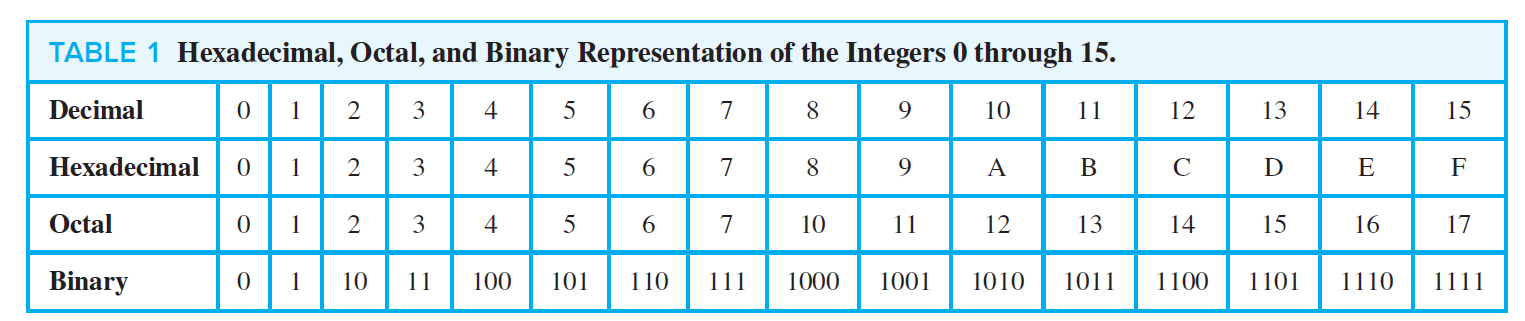
\includegraphics[width=1\linewidth]{converttab.png}
    \caption{Binary, Octal and Hexadecimal Representation}
\end{figure}
The conversion between binary, octal, and hexadecimal systems is straightforward because the bases of these systems (2 for binary, 8 for octal, and 16 for hexadecimal) are related by powers of 2. Specifically:
\begin{itemize}
    \item Octal digits correspond to three binary digits since \(8 = 2^3\). Each octal digit can be directly mapped to a unique combination of three binary bits.
    \item Hexadecimal digits correspond to four binary digits since \(16 = 2^4\). Each hexadecimal digit can be directly mapped to a unique combination of four binary bits.
\end{itemize}
This relationship allows for simple grouping of binary bits into sets of three or four to convert 
to octal or hexadecimal, respectively, without any complex calculation or division. 
\begin{example}
	Find the octal and hexadecimal expansions of $(11\ 1110\ 1011\  1100)_2$ and the binary expansions of $(765)_{8}$ and $(A8D)_{16}$.
\end{example}
\textbf{Solution:} To convert $(11\ 1110\ 1011\  1100)_2$ into octal notation we group the binary digits
into blocks of three, adding initial zeros at the start of the leftmost block if necessary.
These blocks, from left to right, are 011, 111, 010, 111, and 100, corresponding to 3, 7, 2, 7, and 4 respectively. Consequently, we get $(11\ 1110\ 1011\  1100)_2 = (37274)_8$
\par We do the hexadecimal convention in the same way. These blocks, from left to right, are 0011,
1110, 1011, and 1100, corresponding to the hexadecimal digits 3, E, B, and C, respectively. Consequently, $(11\ 1110\ 1011\  1100)_2 = (3EBC)_{16}$
\par \textbf{NOTE: } The conversion could be done inversely in the same way. If the number of bit is not the multiple of 4 when you are converting between 2 and 16 base
number, fill those missing digits/bits with 0.

Whether you noticed or that the base conversion, essentially, is about division and modular arithmetic
that we just learned? The general base conversion algorithm could be simplified to the following algorithm,
where $n$ denotes the number to be converted and $b$ is the target base.
\begin{algorithm}
    \caption{Constructing Base \( b \) Expansions}
    \begin{algorithmic}[H]
    \Procedure{base \( b \) expansion}{$n, b$: positive integers with $b > 1$}
    \State $q \gets n$
    \State $k \gets 0$
    \While{$q \neq 0$}
    \State $a_k \gets q \mod b$
    \State $q \gets \lfloor q / b \rfloor$
    \State $k \gets k + 1$
    \EndWhile
    \State \textbf{return} $(a_{k-1}, \ldots, a_1, a_0)$ \Comment{The base \( b \) expansion of \( n \)}
    \EndProcedure
    \end{algorithmic}
    \end{algorithm}
    \subsection{Operation Algorithms of Number}
        This section discusses algorithm of basic operation between numbers, of base2. 
        In section, we express the binary number in the form of 
        $$a=(a_{n-1}a_{n-2}\ldots a_1a_0)_2,b=(b_{n-1}b_{n-2}\ldots b_1b_0)_2$$
        where $a$ and $b$ each have n bits.
    \subsubsection*{Addition Algorithm}
    Consider the problem of adding two integers in binary notation. A procedure to perform addition can be based on the usual method for adding numbers with pencil and paper. This method proceeds by adding pairs of binary digits together with carries, when they occur, to compute the sum of two integers. This procedure will now be specified in detail.

    To add \( a \) and \( b \), first add their rightmost bits. This gives
    \[
    a_0 + b_0 = c_0 \cdot 2 + s_0,
    \]
    where \( s_0 \) is the rightmost bit in the binary expansion of \( a + b \) and \( c_0 \) is the carry, which is either 0 or 1. Then add the next pair of bits and the carry,
    \[
    a_1 + b_1 + c_0 = c_1 \cdot 2 + s_1,
    \]
    where \( s_1 \) is the next bit (from the right) in the binary expansion of \( a + b \), and \( c_1 \) is the carry. Continue this process, adding the corresponding bits in the two binary expansions and the carry, to determine the next bit from the right in the binary expansion of \( a + b \). At the last stage, add \( a_{n-1} \), \( b_{n-1} \), and \( c_{n-2} \) to obtain \( c_{n-1} \cdot 2 + s_{n-1} \). The leading bit of the sum is \( s_n = c_{n-1} \). This procedure produces the binary expansion of the sum, namely, \( a + b = (s_n s_{n-1} \ldots s_1 s_0)_2 \).
    Consider the binary addition of two numbers, \( 1011_2 \) and \( 1101_2 \).

The addition process is similar to that used in decimal addition, but it is performed in base 2. Below is the columnar addition process:

\begin{center}
\begin{tabular}{ r >{$}r<{$} }
   & 1011_2 \\
  +& 1101_2 \\
  \hline
   & 11000_2 \\
\end{tabular}
\end{center}

Let's perform the addition step by step:

\begin{enumerate}
    \item Start with the rightmost bits (least significant bits). Add \( 1 + 1 \). Since this is base 2, \( 1 + 1 = 10_2 \). Write down the \( 0 \) and carry the \( 1 \) over to the next column.
    \item Move to the next column. Add \( 1 + 0 + 1 \) (including the carry). This equals \( 10_2 \). Write down the \( 0 \) and carry the \( 1 \).
    \item In the next column, add \( 0 + 1 + 1 \). This equals \( 10_2 \). Write down the \( 0 \) and carry the \( 1 \).
    \item For the leftmost bits (most significant bits), add \( 1 + 1 + 1 \). This equals \( 11_2 \). Write down the \( 1 \) and carry the \( 1 \) to a new column to the left.
    \item Write down the carry.
\end{enumerate}
The final result is \( 11000_2 \).

This algorithm's pseudocode is as listed below.
\begin{algorithm}
    \caption{Addition of Integers}
    \begin{algorithmic}[H]
    \Procedure{add}{$a, b$: positive integers}
    \State {the binary expansions of $a$ and $b$ are $(a_{n-1}a_{n-2}\ldots a_1a_0)_2$}
    \State {and $(b_{n-1}b_{n-2}\ldots b_1b_0)_2$, respectively}
    \State $c \gets 0$
    \For{$j \gets 0$ \textbf{to} $n-1$}
        \State $d \gets \left\lfloor (a_j + b_j + c)/2 \right\rfloor$
        \State $s_j \gets a_j + b_j + c - 2d$
        \State $c \gets d$
    \EndFor
    \State $s_n \gets c$
    \State \textbf{return} $(s_{n}s_{n-1}\ldots s_1s_0)_2$ \Comment{the binary expansion of the sum}
    \EndProcedure
    \end{algorithmic}
    \end{algorithm}

    
    \textbf{Time Complexity:}
    The time complexity of the binary addition algorithm is \( O(n) \), where \( n \) is the number of bits in the binary representation of the inputs.
    \begin{proof}
        Consider the binary addition algorithm which consists of a single loop that iterates \( n \) times, where \( n \) is the number of bits in the binary representations of the two integers being added.
        
        Within the loop, the algorithm performs a constant number of operations for each bit:
        \begin{itemize}
            \item An addition of the \( j \)-th bits of the two numbers \( a_j + b_j \).
            \item An addition of the carry from the previous step \( c \).
            \item A division by 2 to compute the new carry \( d \).
            \item A subtraction to determine the \( j \)-th bit of the sum \( s_j \).
            \item An assignment of the new carry \( c \gets d \).
        \end{itemize}
        
        Since each of these operations has a constant time complexity, and they are all executed once for each bit, the overall time complexity of the loop is linear with respect to the number of bits. Therefore, the time complexity of the entire algorithm is \( O(n) \).
        
        Note that this analysis assumes that basic arithmetic operations (addition, division by 2, subtraction) can be performed in constant time.
        \end{proof}
    \subsubsection*{Multiplication Algorithm}
        Using the same representation of binary number $a$ and $b$, we can define binary multiplication
        as $$\begin{aligned}a b & =a\left(b_{0} 2^{0}+b_{1} 2^{1}+\cdots+b_{n-1} 2^{n-1}\right) \\& =a\left(b_{0} 2^{0}\right)+a\left(b_{1} 2^{1}\right)+\cdots+a\left(b_{n-1} 2^{n-1}\right)\end{aligned}$$.
        The binary multiplication algorithm works similarly to traditional pencil-and-paper multiplication, but with binary digits. Given two binary numbers, we multiply each bit of the second number by the first number, shifting the result left for each subsequent bit.
        \begin{algorithm}
            \caption{Addition of Integers}
            \begin{algorithmic}
            \Procedure{ADD}{$a, b$: positive integers}
                \State {the binary expansions of $a$ and $b$ are $(a_{n-1}a_{n-2}\ldots a_1a_0)_2$}
                \State {and $(b_{n-1}b_{n-2}\ldots b_1b_0)_2$, respectively}
                \State $c \gets 0$
                \For {$j \gets 0 \text{ to } n-1$}
                    \State $d \gets \left\lfloor (a_j + b_j + c)/2 \right\rfloor$
                    \State $s_j \gets a_j + b_j + c - 2d$
                    \State $c \gets d$
                \EndFor
                \State $s_n \gets c$
                \State \Return $(s_{n}s_{n-1}\ldots s_1s_0)_2$ \Comment{the binary expansion of the sum}
            \EndProcedure
            \end{algorithmic}
            \end{algorithm}

        \begin{example}
            \textbf{Find the product of \( a = (110)_2 \) and \( b = (101)_2 \).}
            First note that
            \begin{align*}
            a \cdot b_0 \cdot 2^0 &= (110)_2 \cdot 1 \cdot 2^0 = (110)_2, \\
            a \cdot b_1 \cdot 2^1 &= (110)_2 \cdot 0 \cdot 2^1 = (0000)_2, \\
            \text{and} \\
            a \cdot b_2 \cdot 2^2 &= (110)_2 \cdot 1 \cdot 2^2 = (11000)_2.
            \end{align*}
            To find the product, add \( (110)_2, (0000)_2, \) and \( (11000)_2 \). Carrying out these additions (using Algorithm 2, including initial zero bits when necessary) shows that \( ab = (11110)_2 \).

        \textbf{Time Complexity:} The time complexity of binary multiplication is \(O(n^2)\), where \(n\) is the number of bits in the binary numbers. This is because each bit of one number is multiplied by each bit of the other number, resulting in \(n\) multiplications for each of the \(n\) bits.
        \end{example}
    \subsubsection*{Algorithm for Div and Mod}
        The following algorithm is used to find the quotient and remainder of $a \div b$.
        This is a more general algorithm as it could handle the cases where a is negative
    \begin{algorithm}
        \caption{Computing div and mod.}
        \begin{algorithmic}
        \Procedure{division\_algorithm}{$a$: integer, $d$: positive integer}
            \State $q \gets 0$
            \State $r \gets |a|$
            \While{$r \geq d$}
                \State $r \gets r - d$
                \State $q \gets q + 1$
            \EndWhile
            \If{$a < 0$ \textbf{and} $r > 0$}
                \State $r \gets d - r$
                \State $q \gets -(q + 1)$
            \EndIf
            \State \Return $(q, r)$ \Comment{$q = a \div d$ is the quotient, $r = a \mod d$ is the remainder}
        \EndProcedure
        \end{algorithmic}
        \end{algorithm}
    
    \subsection{Modular Exponentiation Algorithm}
    An important application of modular arithmetic is finding \( b^n \bmod m\) efficiently, which is crucial for cryptography. $b^n$ could be a huge
    number that takes a lot of time to calculate, so we need this algorithm to speed up this process. to implement this algorithm, we need to use the
    binary expansion of the number $n=(a_{k-1}\ldots a_1a_0)_2$.
    Since 
    $$
    b^n=b^{a_{k-1}\cdot2^{k-1}+\cdots+a_1\cdot2+a_0}=b^{a_{k-1}\cdot2^{k-1}}\cdots b^{a_1\cdot2}\cdot b^{a_0}.
    $$

    This shows that to compute $b^n$, we need only compute the values of $b,b^2,(b^2)^2=b^4,(b^4)^2=$ $b^8,...,b^{2^k}$.
    Once we have these values, we multiply the terms $b^{2j}$ in this list, where $a_j=1$ .(For efficiency and to reduce space requirements, after multiplying by each term, we reduce the result modulo $m.)$
    \begin{example}
        Compute $4^9$\\
        \textbf{Solution: } To compute $4^9$ we first note that $9 = (1001)_2$, so that $4^9 = 4^8 3^2 4^1$. 
        By successively squaring, we find that $4^2 = 16$, $4^4 = 16^2 = 256$, and $4^8 = (256)^2 = 65536$. Consequently, $4^9 = 4^8 4^2 4^1 = 65536 \cdot 16 \cdot 4 = 4,194,304$. 
    \end{example}
    Now we have already finished the part of algorithm to find $b^n$. With this, we can define the algorithm to find $b^n \bmod m$.
    The pseudocode of the algorithm is in the listing below.
    \begin{algorithm} \label{modulare}
        \caption{Fast Modular Exponentiation.}
        \begin{algorithmic}
        \Procedure{modular exponentiation}{$b$: integer, $n = (a_{k-1}a_{k-2} \ldots a_1a_0)_2$, $m$: positive integers}
        \State $x := 1$
        \State $power := b \mod m$
        \For{$i := 0$ to $k-1$}
        \If{$a_i = 1$} \textbf{then} $x := (x \cdot power) \mod m$
        \EndIf
        \State $power := (power \cdot power) \mod m$
        \EndFor
        \State \textbf{return} $x$ {$x$ equals $b^n \mod m$}
        \EndProcedure
        \end{algorithmic}
    \end{algorithm}

    \begin{example}
        Find the value of $3^{644} \mod 645$ using the Algorithm.
        
        \textit{Solution:} The algorithm starts by initializing $x = 1$ and $power = 3 \mod 645 = 3$. It then calculates
        $3^{2j} \mod 645$ for $j = 1, 2, \ldots, 9$ by repeatedly squaring and reducing modulo 645. When the $j$th bit of 644 
        (in binary, $(1010000100)_2$) is 1, the algorithm multiplies the current $x$ by $3^{2j} \mod 645$ and reduces the product modulo 645. The steps are as follows:
        
        \begin{tabular}{ll}
        $i = 0$: & $a_0 = 0$, so $x = 1$ and $power = 3^2 \mod 645 = 9$. \\
        $i = 1$: & $a_1 = 0$, so $x = 1$ and $power = 9^2 \mod 645 = 81$. \\
        $i = 2$: & $a_2 = 1$, so $x = 1 \cdot 81 \mod 645 = 81$ and $power = 81^2 \mod 645 = 111$. \\
        $i = 3$: & $a_3 = 0$, so $x = 81$ and $power = 111^2 \mod 645 = 66$. \\
        $i = 4$: & $a_4 = 0$, so $x = 81$ and $power = 66^2 \mod 645 = 486$. \\
        $i = 5$: & $a_5 = 0$, so $x = 81$ and $power = 486^2 \mod 645 = 126$. \\
        $i = 6$: & $a_6 = 0$, so $x = 81$ and $power = 126^2 \mod 645 = 396$. \\
        $i = 7$: & $a_7 = 1$, so $x = (81 \cdot 396) \mod 645 = 471$ and $power = 396^2 \mod 645 = 81$. \\
        $i = 8$: & $a_8 = 0$, so $x = 471$ and $power = 81^2 \mod 645 = 111$. \\
        $i = 9$: & $a_9 = 1$, so $x = (471 \cdot 111) \mod 645 = 36$.
        \end{tabular}
        
        Thus, the value of $3^{644} \mod 645$ is 36.
        \end{example}

        \paragraph{Time Complexity of Algorithm 5}
        The time complexity of Algorithm \ref{modulare} is determined by the number of iterations in the for loop, which is equal to the number of 
        bits in the binary representation of the exponent $n$. In each iteration, the algorithm performs a constant number of modular multiplications and 
        squarings. Therefore, the time complexity of Algorithm \ref{modulare} is $O(\log n)$, where $n$ is the exponent. This is a significant improvement over the naive method of modular exponentiation, 
        which has a time complexity of $O(n)$. The fast modular exponentiation algorithm is particularly useful in cryptographic applications, such as the RSA algorithm, 
        where the exponents are typically large numbers.

        To prove that the time complexity of Algorithm \ref{modulare} is $O(\log n)$, we can analyze the number of operations performed by the algorithm in relation to the size of the input exponent $n$.

        \begin{proof}
        Let $n$ be the exponent in the modular exponentiation problem, and let $k$ be the number of bits in the binary representation of $n$. We can express $n$ as:

        \[n = \sum_{i=0}^{k-1} a_i \cdot 2^i, \text{ where } a_i \in \{0, 1\}\]

        The algorithm iterates through the bits of $n$ from right to left (from the least significant bit to the most significant bit). In each iteration, the algorithm performs the following operations:

        \begin{enumerate}
        \item If $a_i = 1$, it performs a modular multiplication to update the value of $x$.
        \item It performs a modular squaring to update the value of $\textit{power}$.
        \end{enumerate}

        The modular multiplication and squaring operations can be performed in $O(1)$ time using a constant number of arithmetic operations modulo $m$.

        Since the algorithm iterates through all $k$ bits of $n$, the total number of iterations is $k$. Therefore, the time complexity of the algorithm is proportional to $k$, which is the number of bits in the binary representation of $n$.

        We know that the number of bits in the binary representation of $n$ is $\lfloor \log_2 n \rfloor + 1$. Thus, $k = O(\log n)$.

        Consequently, the time complexity of Algorithm \ref{modulare} is $O(\log n)$.
        \end{proof}

        This logarithmic time complexity makes Algorithm \ref{modulare} (fast modular exponentiation) much more efficient than the naive method of modular exponentiation, which has a linear time complexity of $O(n)$.
    \subsection{Exercises}



\section{Primes and Greatest Common Divisors}
        In previous chapter, we learned the properties of division and divisibility, as well as
        modular arithmetic. These are the most essential parts of the whole number theory. In this section
        , we will discuss primes and its property. Prime is not something unfamiliar to us, since some may
        even have learned that from the kindergarten or primary school. We will look into the Algorithms
        that could help is find primes and delve into the algebraic properties of prime later. All these
        are foundations of cryptography.
    \subsection{Primes and Related Algorithms}
        To learn prime, of course we need to recap on its definition.
        \begin{definition}[Prime Number]  
            An integer $p$ greater than 1 is called prime if the only positive factors of $p$ are 1 and $p$.
            A positive integer that is greater than 1 and is not prime is called \textbf{composite}.
        \end{definition}    
        Note that, by this definition, 1 is not a prime, as it is only 1 as the only factor.

        The reason why prime numbers are so fascinating to mathematicians is that they have so many
        interesting and unique property, even except for what we have seen in its definition. Below is what we call the fundamental theorem of arithmetic.
        \begin{theorem}[The Fundamental Theorem of Arithmetic]
            For every integer $n > 1$, there exists a unique factorization into prime numbers, up to the order of the factors. Specifically, $n$ can be expressed as
            \[ n = p_1^{a_1} \cdot p_2^{a_2} \cdot \ldots \cdot p_k^{a_k} \]
            where $p_1 < p_2 < \ldots < p_k$ are prime numbers and $a_1, a_2, \ldots, a_k$ are positive integers. This factorization is unique, apart from the order of the prime factors.
        \end{theorem}
        \begin{proof}
            We prove the theorem in two parts: existence and uniqueness.
            
            \textbf{Existence:} We prove by mathematical induction that every integer greater than 1 can be written as a product of primes.
            
            \textit{Base Case:} For $n = 2$, the statement holds true since 2 is itself a prime number.
            
            \textit{Inductive Step:} Assume the statement holds for all integers greater than 1 and less than $n$. Now consider the integer $n$.
            \begin{itemize}
                \item If $n$ is prime, then it is trivially a product of primes (itself).
                \item If $n$ is not prime, it can be written as $n = a \cdot b$ where $1 < a, b < n$. By the inductive hypothesis, both $a$ and $b$ can be factored into a product of primes. Therefore, $n$ can also be expressed as a product of primes by combining the prime factorization of $a$ and $b$.
            \end{itemize}
            This completes the proof of existence.
            
            \textbf{Uniqueness:} Assume, for the sake of contradiction, that there are two distinct prime factorization of $n$:
            \[ n = p_1^{a_1} \cdot p_2^{a_2} \cdot \ldots \cdot p_k^{a_k} = q_1^{b_1} \cdot q_2^{b_2} \cdot \ldots \cdot q_m^{b_m} \]
            where $p_i$ and $q_j$ are prime numbers, and $a_i, b_j$ are positive integers.
            To proceed to the rest of the proof, we need to use Euclid's lemma.

            \textbf{lemma:}

                Let \(p\) be a prime number. If \(p\) divides the product \(ab\), where \(a\) and \(b\) are integers, then \(p\) divides \(a\) or \(p\) divides \(b\).
            \begin{proof}
                Assume \(p\) is a prime that divides \(ab\) but does not divide \(a\). We need to show that \(p\) must divide \(b\).

                Since \(p\) does not divide \(a\), the greatest common divisor (gcd) of \(a\) and \(p\) is 1, i.e., \(\text{gcd}(a, p) = 1\). According to Bezout's identity, there exist integers \(x\) and \(y\) such that:

                \[ax + py = 1\]

                Multiplying both sides of the equation by \(b\), we get:

                \[abx + pby = b\]
                \begin{remark}
                    If this proof is not yet understandable for you, skip it, and check it back after we go over the rest of this chapter about linear combination and this theorem.
                \end{remark}
                Since \(p\) divides \(ab\) (by assumption), \(p\) divides \(abx\). Also, \(p\) obviously divides \(pby\). Hence, \(p\) divides the sum \(abx + pby\), which means \(p\) divides \(b\).

                This completes the proof, showing that if \(p\) divides \(ab\) and does not divide \(a\), then \(p\) must divide \(b\), in accordance with Euclid's lemma.
            \end{proof}
            By Euclid's lemma, if a prime divides the product of two numbers, it must divide at least one of those numbers. Thus, $p_1$ must divide some $q_j$ on the right-hand side. Since $q_j$ is prime, we conclude that $p_1 = q_j$. Applying this argument symmetrically and repeatedly, we find that each set of prime factors must be identical to the other, contradicting the assumption of two distinct factorization.
            
            Therefore, the prime factorization of any integer greater than 1 is unique, up to the order of the factors, which completes the proof of the Fundamental Theorem of Arithmetic.
            \end{proof}
            
        \begin{example}
            100 can be taken as $100 = 2\cdot 2\cdot 5\cdot 5 = 2^2\cdot 5^2$.
            Both 2 and 5 are primes.
        \end{example}

        Now that we know these interesting properties of prime and its significance, how do we find
        primes, not just correctly, but also efficiently? The most basic algorithm that anyone
        could find is that we can actually check numbers one by one. To find whether an integer $n$ is prime, what we need to do is to check every number from 2 to $n-1$, and use them to divide $n$ one by one. If anyone of them divides $n$, then $n$ is not prime, and vice versa.
        \subsubsection*{Trial Division}
        We actually can apply a more efficient way to determine whether an integer is prime or not.
        Considering the following theorem.
        \begin{theorem}
            If \( n \) is a composite integer, then \( n \) has a prime divisor less than or equal to \( \sqrt{n} \).
        \end{theorem}
        \begin{proof}
            If \( n \) is composite, by the definition of a composite integer, we know that it has a factor \( a \) with \( 1 < a < n \). Hence, by the definition of a factor of a positive integer, we have \( n = ab \), where \( b \) is a positive integer greater than 1. We will show that \( a \leq \sqrt{n} \) or \( b \leq \sqrt{n} \). If \( a > \sqrt{n} \) and \( b > \sqrt{n} \), then \( ab > \sqrt{n} \cdot \sqrt{n} = n \), which is a contradiction. Consequently, \( a \leq \sqrt{n} \) or \( b \leq \sqrt{n} \). Because both \( a \) and \( b \) are divisors of \( n \), we see that \( n \) has a positive divisor not exceeding \( \sqrt{n} \). This divisor is either prime or, by the fundamental theorem of arithmetic, has a prime divisor less than itself. In either case, \( n \) has a prime divisor less than or equal to \( \sqrt{n} \).
            \end{proof}
        Below is the pseudocode for this procedure.
        \begin{algorithm}
            \caption{Primality Test Using Trial Division}
            \begin{algorithmic}[1]
            
            \Function{IsPrime}{$n$}
                \If{$n \leq 1$}
                    \State \Return \textbf{false}
                \EndIf
                \For{$i \gets 2$ \textbf{to} $n-1$}
                    \If{$n \mod i = 0$}
                        \State \Return \textbf{false}
                    \EndIf
                \EndFor
                \State \Return \textbf{true}
            \EndFunction
            
            \end{algorithmic}
            \end{algorithm}
        \begin{example}
            Show that $\sqrt{105}$ is prime.
        \end{example} 
        textbf{Solution:} Primes less than $\sqrt{105}$ are 2, 3, 5, 7. 101 is not divisible
        by any of them, so it is not composite, and thus it is prime.

        We also need an efficient algorithm to factorize a give number to primes. Here is how is
        works. It works as follows.
        \begin{algorithm}
            \caption{Prime Factorization}
            \begin{algorithmic}[H]
            
            \Function{PrimeFactorization}{$n$}
                \State $factors \gets \text{an empty list}$
                \For{$p \gets 2$ \textbf{to} $\infty$}
                    \While{$n \mod p == 0$}
                        \State Add $p$ to $factors$
                        \State $n \gets n / p$
                    \EndWhile
                    \If{$p > n / p$}
                        \State \textbf{break}
                    \EndIf
                \EndFor
                \If{$n > 1$}
                    \State Add $n$ to $factors$
                \EndIf
                \State \Return $factors$
            \EndFunction
            
            \end{algorithmic}
            \end{algorithm}
        \begin{example}
            Find the prime factorization of 8964.
        \end{example}
        \textbf{Solution:}

        \begin{enumerate}
            \item 8964 is even, so start with 2: \( 8964 \div 2 = 4482 \).
            \item 4482 is also even, divide by 2 again: \( 4482 \div 2 = 2241 \).
            \item 2241 is not divisible by 2. The next primes to try are 3, 5, 7, 11, and so on. We find that 2241 is not divisible by any of these primes until we reach 31.
            \item 2241 divided by 31 gives us 71, which is a prime number.
        \end{enumerate}
        
        Thus, the prime factorization of 8964 is \( 2 \times 2 \times 31 \times 71 \), or in exponent form, \( 2^2 \times 31 \times 71 \).

        There are also other method to finding prime numbers or tell whether a number is prime or not. If you are willing
        to delve into it, you may check \href{https://en.wikipedia.org/wiki/Sieve_of_Eratosthenes}{Sieve of Eratosthenes}, 
        \href{https://en.wikipedia.org/wiki/Sieve_of_Atkin}{Sieve of Ktkin}. These are only small part of all possible method,
        which we will learn later, such as Fermat's Little Theorem in solving congruence, as well as Monte Carlo method in probability.

    \subsection{Greatest Common Divisors and Least Common Multiples}
        Now we will discuss yet another primary school topic, GCD and LCM. Briefyly recap their definitions:
        \begin{definition}[Greatest Common Divisior]
            Let $a$ and $b$ be integers, not both zero. The largest integer $d$ such that $d \mid a$ and 
            $d \mid b $ is called the greatest common divisor of $a$ and $b$. The greatest common divisor of 
            $a$ and $b$ is denoted by gcd$(a, b)$.
        \end{definition}

    \begin{example}
        Find gcd$(12, 24)$ and gcd$(17, 22)$.

        These are easy-to-solve problems. The largest number that divides 12 and 24 is 6, so gcd$(12,24)=6$,while 
        17 and 22 do not have common divisor other than 1, so gcd$(17, 22)=1$.
    \end{example}

    For 17 and 22, we have gcd$(17, 22)=1$. In this case, we call that they are \textbf{Relatively Prime}, because
    their greatest common divisor is 1.

    We can generalize this idea to pairwise Relatively prime.
    \begin{definition}[Pairwise Relatively Prime]
        The integers $a_1,a_2,...,a_n$ are pairwise relatively prime if $\gcd(a_i,a_j)=1$ whenever $1\leq i<$ $j\leq n.$
    \end{definition}
    For example, 9, 16, 23 are pairwise relatively prime, becuase gcd$(9,16)=0$, gcd$(9,23)=0$, gcd$(16,23)=0$. So we could
    say that a sequence of number is pairwise relatively prime if and only if any combination of 2 of the numbers in The
    sequence $a$, $b$, has gcd $(a,b)=1$.

    The other way to find gcd of two number is using their prime factorization. Suppose that the prime factorizations of the positive integers $a$ and 
    $b$ are $$a=p_1^{a_1}p_2^{a_2}\cdots p_n^{a_n},b=p_1^{b_1}p_2^{b_2}\cdots p_n^{b_n},$$.
    where each exponent is a nonnegative integer, and where all primes occurring in the prime factorization of either 
    $a$ or $b$ are included in both factorizations, with zero exponents if necessary. Then gcd$(a, b)$ is given by
    $$\gcd(a,b)=p_1^{\min(a_1,b_1)}p_2^{\min(a_2,b_2)}\cdotp\cdotp\cdotp p_n^{\min(a_n,b_n)},$$
    where $\min(x,y)$ represents the minimum of the two numbers $x$ and y. To show that this formula for 
    $\gcd(a,b)$ is valid, we must show that the integer on the right-hand side divides both $a$ and $b$, and that no larger integer also does. This integer does divide both $\alpha$ and $b$, because the power of each prime in the factorization does not exceed the power of this prime in either the factorization of $a$ or that of $b$. Further, no larger integer can divide both $\alpha$ and $b$, because the exponents of the primes in this factorization cannot be increased, and no other primes can be included.
    \begin{example}
        Find $\gcd(100, 250)$.

        $$\gcd(120,500)=2^{\min(3,2)}3^{\min(1,0)}5^{\min(1,3)}=2^23^05^1=20.$$
    \end{example}  

    This method could be finetuned to find the least common multiple of two integers. Still according to the fundamental
    theorem of arithmetic, every integer could find a unique factorization as product of prime numbers.
    \begin{definition}
        The least common multiple of the positive integers $a$ and $b$ is the smallest positive integer that is 
        divisible by both $a$ and $b$. The least common multiple of $a$ and $b$ is denoted by lcm$(a, b)$.
    \end{definition}
        Suppose the prime factorizations of \(a\) and \(b\) are given by
        \[ a = p_1^{a_1} p_2^{a_2} \ldots p_n^{a_n}, \quad b = p_1^{b_1} p_2^{b_2} \ldots p_n^{b_n}, \]
        where \(a_i\) and \(b_i\) are the exponents of the prime factors of \(a\) and \(b\), respectively.

        The product \(ab\) can be expressed as a prime factorization:
        \[ ab = p_1^{a_1+b_1} p_2^{a_2+b_2} \ldots p_n^{a_n+b_n}. \]

        From this, we can deduce that any common multiple of \(a\) and \(b\) must be a product of their prime factors raised to at least the maximum exponent found in either \(a\) or \(b\). Therefore, the \(\text{lcm}(a, b)\) can be expressed as
        \[ \text{lcm}(a, b) = p_1^{\max(a_1,b_1)} p_2^{\max(a_2,b_2)} \ldots p_n^{\max(a_n,b_n)}. \]
        This ensures that \(\text{lcm}(a, b)\) is divisible by both \(a\) and \(b\), and it is the smallest such number with this property.

    \begin{example}
        Find lcm$(120, 500)$.
        $$\text{lcm}(120,500)=2^{\max(2,3)}3^{\max(1,0)}5^{\max(1,3)} = 8\times 3 \times 125= 3000$$
    \end{example}
    Have you noticed, that $ab$ is actually the product of $\text{lcm}(a,b)$ and $\gcd(a,b)$? Becuase the order of each
    term in the prime factorization of $ab$ is a sum of two number, what ever which number is the maximum of the minimum,
    we always have the order of $a_n+b_n$. For 120 and 500 we have 
    $$ab = 120\times 500 = 60000 = \text{lcm}(a,b)\times \gcd(a,b) = 3000\times 20$$

    \begin{theorem}
        Let $a$ and $b$ be positive integers. Then $ab= \gcd ( a, b) \cdot $lcm$( a, b).$
    \end{theorem}

    \subsubsection*{The Euclidean Algorithm}

    \subsubsection*{Greatest Common Divisors as Linear Combinations}
        The greatest common divisor of two integers $a$ and $b$ can be expressed in the form
        $$sa + tb$$
        where $s$ and $t$ are integers. In other words, $\gcd(a, b)$ can be expressed as a linear combination with 
        integer coefficients of $a$ and $b$. 

        This property of GCD is exactlly the Bézout's Theorem, which states that:
        \begin{theorem}[Bézout's Theorem]\label{Bezout}
            Let $a$ and $b$ be integers, not both zero. There exist integers $x$ and $y$ such that
            \[
            ax + by = \gcd(a, b),
            \]
            where $\gcd(a, b)$ denotes the greatest common divisor of $a$ and $b$. The integers $x$ and $y$ are known as Bézout coefficients.
            the equation$ \gcd(a, b) = sa + tb$ is called Bézout's identity.
        \end{theorem}
        \begin{proof}
            The proof of Bézout's identity uses the property that for nonzero integers $a$ and $b$, dividing $a$ by 
            $b$ leaves a remainder of $r_1$ strictly less than $|b|$ and $\gcd(a,b)=$.
            $\gcd(r_1,b)$.Then by repeated applications of the Euclidean division algorithm, we have
            $a=bx_1+r_1$, $0<r_1<|b|$, $b=r_1x_2+r_2$, $0<r_2<r_1$,
            $$r_{n-1}=r_nx_{n+1}+r_{n+1},\quad0<r_{n+1}<r_n$$
            $$r_n=r_{n+1}x_{n+2}$$

            where the $r_{n+1}$ is the last nonzero remainder in the division process. Now, as illustrated in the example above, we can use the second to last equation to solve for $r_{n+1}$ as a combination of $r_n$ and $r_{n-1}$. Unfolding this, we can solve for $r_n$ as a combination of $r_{n-1}$ and $r_{n-2}$ etc. until we eventually write $r_{n+1}$ as alinear
            combination of $a$ and $b$. Since $r_{n+1}$ is the last nonzero remainder in the division process, it is the greatest common divisor of $a$ and $b$,which proves Bézout's identity.
        \end{proof}
        \begin{remark}
            Bezout's Theorem is closely related to Linear Diophantine Equations, which we will
            discuss further in solving linear congruence.
        \end{remark}

        We use a example to explain further on the theorem. Recall that Euclidean algorithm is actually a recursive algorithm, to find
        gcd of $a$ and $b$, it requires multiple usage of the algorithm.
        \begin{example} 
            Use the Euclidean algorithm to find the greatest common divisor of 1022 and 400.
        \end{example}   
        \textbf{Solution:}
$$
        \begin{aligned}\\
            1022&=2\times400+222\\
            400&=1\times 222+178\\
            222&=1\times 178+44\\
            178&=4\times 44+2\\
            44&=22\times2+0
            \end{aligned}
   $$ 
        In this way, we find $\gcd(1022,400)=2$ easily. Writing the step-by-step of using Euclidean like this is what we call \textbf{the
        Extended Euclidean Algorithm}. 

        Notice further that as the terms in the extended algorithm could be expressed by previous lines, we can finally get a linear combination
        of the gcd over 1022 and 400. In this case, we have $2 = 23\times 400-9\times 1022$.

        Now consider an equivalent expression for the problem.  Find integers $a$ and $b$ such that $\gcd(1022, 400) = a \times 1022 + b \times 400$.
        In this case, we do exactly the same thing, and straightforward, we have $a=-9$ and $b=23$.

        There is still another equivalent expression to this, and it will be discussed with linear congruence in the next section.



    \subsection{Exercises}


    
    
    \section{Solving Congruence}
        Earlier in this chapter, we introduced divisibility, and thus defined division and modular arithmetic, as well as modular congruence.
        We have also introduced algebraic properties of congruence, and surprisingly, many of which are just like "copying" from the real number
        , or we generally say, normal algebra system. Now think about how we learn math for real number. We learnt all the way from basic operations, and finally we just do not use the numbers anymore in the expression, but in stead, letters, and we call this algebra. Now that modular congruence
        shares so many basic properties with that, can we extend to more algebra on modular congruence? This section introduces solving equation, or only
        linear equations, of modular congruence, and it has much to do with Euclidean algorithm.
            

        \subsection{Linear Congruence}
            \begin{definition}[Linear Congruence]
                Congruence of the form as follows
                $$ax \equiv b (\bmod m)$$
                is called \textbf{Linear Congruence}, where $a, b,  m \in \mathbb{Z}^+$, and $x$ is the variable to be solved.
                To solve this congruence, we need to find $\bar{a}$, which we call \textbf{inverse of a modulo m} if $a$, such that
                $a\bar{a} \equiv 1 (\bmod m)$.
            \end{definition}
        If we are to find the $x$ of a given expression, what kind of solution we will get? Do we get 
        specific solution or infinitely many solutions? The fact is that we will get infinitely many
        solutions, since modular congruence has periodicity.

        \begin{theorem}[Existence of Inverses Theorem]\label{exist_inverse}
            If \( a \) and \( m \) are relatively prime integers and \( m > 1 \), then an inverse of \( a \) modulo \( m \) exists. Furthermore, this inverse is unique modulo \( m \). (That is, there is a unique positive integer \( \bar{a} \) that is an inverse of \( a \) modulo \( m \) and every other inverse of \( a \) modulo \( m \) is congruent to \( \bar{a} \) modulo \( m \).)
            \end{theorem}
            
            \begin{proof}
            By Bezout's Theorem, because \( \gcd(a, m) = 1 \), there are integers \( s \) and \( t \) such that
            \[
            sa + tm = 1.
            \]
            This implies that
            \[
            sa + tm \equiv 1 \pmod{m}.
            \]
            Because \( tm \equiv 0 \pmod{m} \), it follows that
            \[
            sa \equiv 1 \pmod{m}.
            \]
            Consequently, \( s \) is an inverse of \( a \) modulo \( m \).

            Now we try to prove the uniqueness of $s$ as an inverse of \( a \) modulo \( m \).
            Suppose there are other integers than $s$ ($x$) that satisfies  
            \[ xa \equiv 1 \pmod{m} \text{ and } x \neq s + km\]
            So, by definition of modular congruence we have $xa \bmod m = 1$ and $sa \bmod m = 1$, which
            gives
            $$xa \equiv sa \pmod m$$
            So $m\mid xa - sa$, and this means that $xa - sa = km$ for some integer $k$ must be true.
            If that is true, then $x-s$ is also multiple of $m$, which means $x\equiv s \pmod m$.
            Now recall our assumption that $x\neq s + km$, so $x = s + km$ for some integer $k$ refutes
            our assumption. Therefore, there is a unique positive integer $\bar{a}$ that is an inverse of a 
            modulo $m$ and every other inverse of $a$ modulo $m$ is congruent to $\bar{a}$ modulo m.
            \end{proof}
        
        \begin{example}
            Find an inverse of 101 modulo 5000.
        \end{example}
        \paragraph{Solution:}
we present all steps used to compute an inverse of 101 modulo 5000. First, we use the Euclidean algorithm to show that $\gcd(101, 5000) = 1$. Then we will reverse the steps to find B\'ezout coefficients $a$ and $b$ such that $101a + 5000b = 1$. It will then follow that $a$ is an inverse of 101 modulo 5000. The steps used by the Euclidean algorithm to find $\gcd(101, 5000)$ are
\begin{align*}
5000 &= 49 \cdot 101 + 51 \\
101 &= 1 \cdot 51 + 50 \\
51 &= 1 \cdot 50 + 1 \\
50 &= 50 \cdot 1.
\end{align*}
Because the last nonzero remainder is 1, we know that $\gcd(101, 5000) = 1$. We can now find the Bezout coefficients for 101 and 5000 by working backwards through these steps, expressing the gcd of 101 and 5000 as $1$ in terms of each successive pair of remainders. In each step we eliminate the remainder by expressing it as a linear combination of the divisor and the dividend. We obtain
\begin{align*}
1 &= 51 - 1 \cdot 50 \\
&= 51 - 1 \cdot (101 - 1 \cdot 51) \\
&= 2 \cdot 51 - 101 \\
&= 2 \cdot (5000 - 49 \cdot 101) - 101 \\
&= 2 \cdot 5000 - 99 \cdot 101.
\end{align*}

That $-99 \cdot 5000 + 2 \cdot 101 = 1$ tells us that $2$ and $-99$ are Bezout coefficients of 5000 and 101, and $-99$ is an inverse of 101 modulo 5000.
        %\subsubsection*{Arithmetic of Large Numbers}
    \begin{example}
        What are the solutions of the linear congruence $101x \equiv 3 \pmod {5000}$?
    \end{example}
    We know that -99 is a modular inverse of $101 \bmod 5000$. So we multiply the inverse on the both
    side, this gives
    $$-99 \cdot 101x \equiv -99\cdot 3 \pmod {5000} $$
    $-99\cdot 101 \equiv 1 \pmod{5000}$, so $x\equiv -99 \cdot3 \pmod{5000}$.
    From here we can see that $x$ is not a single number, but a set of numbers. We can have$x = -297, -5293, 4703\cdots$.
    So the general solution $x$ is $x = x_0 + km$, where $k$ is some integer, and $x_0$ is one of the specific solution we can
    find.

    Great, now you can solve any solutions for any linear congruence, as long as it is solvable (has inverse).
    But can we generalize this problem? Because in the previous discussion of solving linear congruence and
    finding the inverse are all based on the condition that the two numbers are coprime, i.e., $\gcd(a,b)=1$.
    What will be the case when they are not coprime?

    Actually, solving linear congruence is a subset of a greater concept, \textbf{Diophantine Equation}.
    \begin{definition}[Diophantine Equation]
        A Diophantine equation is an equation or a system of equations that allows for polynomial expressions in several variables and requires the solutions to be integers. These equations are studied within number theory and are named after Diophantus of Alexandria, a Greek mathematician. Specifically,
        a Diophantine equation can be interpreted by the following expression.
        $$a_{1}x_{1}^{b_{1}}+a_{2}x_{2}^{b_{2}}+......+a_{n}x_{n}^{b_{n}}=c$$
        Where $a$, $b$, $x$, $c \in \mathbb{Z}$. 
    \end{definition}
    You may realize at the first glance that this equation is hard to solve and has infinitely many
    solutions, because for the most basic system of linear equation, we can only get specific solution
    when the number of unknowns is equal to the number of equations in the system. But no worries,
    we discuss only the simplest form of this type of equation for now, which is
    $$ax+by=c \text{.}$$
    Isn't it familiar to you? This is exactly what were shown in Bezout's Theorem (you may check theorem \ref{Bezout})
    This means that, as long as we are finding the relation between between a pair of number $a,b$ with their
    GCD, we are doing exactly the same thing as solving linear congruence, because the latter is
    a subset of the former, as Diophantine equation.

    Now let's work out the general solution of such equation.
    Consider the linear Diophantine equation

\begin{equation}
ax + by = c
\end{equation}

where \(a\), \(b\), and \(c\) are given integers, and \(x\) and \(y\) are unknown integers that we want to solve for. 

\textbf{Step 1: Finding a particular solution}

By the Extended Euclidean Algorithm, we can find integers \(x_0\) and \(y_0\) such that

\begin{equation}
ax_0 + by_0 = \gcd(a, b)
\end{equation}

\textbf{Step 2: The general solution form}

If \(c\) is a multiple of \(\gcd(a, b)\), say \(c = k \cdot \gcd(a, b)\), then by multiplying the equation \(ax_0 + by_0 = \gcd(a, b)\) by \(k\), we get a particular solution to \(ax + by = c\):

\begin{equation}
ax_0k + by_0k = ck
\end{equation}

Now, consider that for any integer \(t\), the following holds:

\begin{equation}
a(x_0 + tb/d) + b(y_0 - ta/d) = ax_0 + by_0 = ck
\end{equation}

where \(d = \gcd(a, b)\). 

This is because the multiples of \(b/d\) added to \(x\) and multiples of \(a/d\) subtracted from \(y\) will cancel each other out when multiplied by \(a\) and \(b\), respectively.

\textbf{Step 3: General solution}

Thus, the general solution to the equation \(ax + by = c\) can be expressed as:

\begin{equation}
x = kx_0 + t\left(\frac{b}{d}\right)
\end{equation}

\begin{equation}
y = ky_0 - t\left(\frac{a}{d}\right)
\end{equation}

where \(t, k\) are any integer and $d = \gcd(a,b)$. This represents an infinite set of solutions if \(a\) and \(b\) are coprime.
\begin{corollary}[Solvability of Linear Diophantine Equation]
    Now consider the cases for solutions, when $a,b$ are coprime ($\gcd(a,b)=1$), there must be integer solutions for the equation,
as shown in the proof, because 1 is a divisor of any integer. However, when $c$ is not a multiple
of $\gcd(a, b)$, we cannot find any integer solution. As for other general cases, i.e., $\gcd(a, b)\neq 1$,
but $\gcd(a,b)\mid c$, there are integer solutions.
\end{corollary}

Now that we have known the idea of Diophantine Equation, we can relate the concept to linear
congruence easily. 
\begin{proposition}[Linear Congruence is a subproblem of Douphantine Equation]
    Solving linear congruence is a subproblem of solving linear Diophantine equation.
    Suppose we are looking for linear combination of $c=sa+tb$, which is equivalent
to solving this Diophantine equation. This is equivalent to find $ax\equiv c \pmod b$.
\end{proposition}
\begin{proof}
    $ax\equiv c \pmod b$ means that $ax \bmod b = c \bmod b$. By division algorithm
    $ax = q_1b + r$, $c = q_2b + r$, where $q$ is the quotient and $q\in \mathbb{Z}$. 
    $c-q_2b = ax-q_1b$, and thus $c = ax + (q_2-q_1)b$, where $a, (q_2-q_1)\in \mathbb{Z}$.
    So we have shown that solving linear congruence could be treated as solving a Diophantine Equation.
\end{proof}
\begin{example}
    Solve $400z\equiv 8 (\bmod1022)$
\end{example}
\textbf{Solution:} 

    We can straightaway treat it as solving the Diophantine equation
    $$8 = 400x + 1022y$$
    We need to know their gcd, so we use extended Euclidean algorithm.
   $$ \begin{aligned}
        1022&=2\times400+222\\
        400&=1\times 222+178\\
        222&=1\times 178+44\\
        178&=4\times 44+2\\
        44&=22\times2+0
        \end{aligned}$$
    
        By Bezout theorem, we use substitution repetitively to get the linear combination of
        their gcd in terms of 400 and 1022, which is $2 = 23\times 400 -9\times 1022$.
        Because 8 is multiple of 2, so we can get $z$ by $8 = -36\times 1022 + 92\times 400$, 
        which is a set of specific solution ($x = 92, y=-36$).

        With the specific solution, we can get the general solution:
        $$ \begin{aligned}\\
            x&=k\cdot 92+t(\frac{1022}{\gcd(400,1022)})\\
            y&=k\cdot(-36)+t(\frac{400}{\gcd(400,1022)} )
            \end{aligned}$$
        
        \subsection{The Chinese Remainder Theorem}
        In the last section, we relate linear congruence to linear equation. Now we will try to relate it to system of linear equations.
        Recall that a \textit{system of linear equations} is a collection of one or more linear equations involving the same variables. 
        \begin{definition}[System of Linear Equations]
        In the context of real numbers, a system of $n$ linear equations in $n$ unknowns $x_1, x_2, \ldots, x_n$ can be written as:
        \begin{align*}
        a_{11}x_1 + a_{12}x_2 + \cdots + a_{1n}x_n &= b_1 \\
        a_{21}x_1 + a_{22}x_2 + \cdots + a_{2n}x_n &= b_2 \\
        \vdots &\\
        a_{n1}x_1 + a_{n2}x_2 + \cdots + a_{nn}x_n &= b_n
        \end{align*}
        where $a_{ij}$ and $b_i$ are real numbers.
        \begin{remark}
            Just a kind reminder that "Linear" basically means the order of polynomial is at most 1, just in case some don't know
            the definition.
        \end{remark}
        \end{definition}
        \begin{definition}[System of Linear Congruences]
        Similarly, a \textit{system of linear congruences} is a collection of linear congruences in the same variables over a ring of integers modulo $m$. A system of $n$ linear congruences in $n$ unknowns $x_1, x_2, \ldots, x_n$ can be written as:
        \begin{align*}
        a_{11}x_1 + a_{12}x_2 + \cdots + a_{1n}x_n &\equiv b_1 \pmod{m_1} \\
        a_{21}x_1 + a_{22}x_2 + \cdots + a_{2n}x_n &\equiv b_2 \pmod{m_2} \\
        \vdots &\\
        a_{n1}x_1 + a_{n2}x_2 + \cdots + a_{nn}x_n &\equiv b_n \pmod{m_n}
        \end{align*}
        where $a_{ij}$, $b_i$, and $m_i$ are integers. The goal in both cases is to find values for the unknowns that simultaneously 
        satisfy all the equations or congruences in the system.
        \end{definition}
        Actually, we cannot solve such complex problems, which  requires further knowledge on matrix and linear algebra. However, just like
        what we do to Diophantine Equations, we are trying to find solution for a specific case of basic form, which, in this case, is 
        discussed in \textbf{Chinese Remainder Theorem}.
        In the first century, the Chinese mathematician Sun-Tsu asked: 
        There are certain things whose number is unknown. When divided by 3, the remainder is 2; when divided by 5, the remainder is 3; 
        and when divided by 7, the remainder is 2. What will be the number of things?

        This problem could be transfered in the a system of linear congruences that
        $${\begin{array}{c}x\equiv2\pmod{3}\\x\equiv3\pmod{5}\\x\equiv2\pmod{7}\end{array}}$$
        The algorithm to find the solution for such problem is known as Chinese Remainder Theorem.
        \begin{theorem}[Chinese Remainder Theorem]
            Let $m_1,m_2,...,m_n$ be pairwise relatively prime positive integers greater than one and $a_1,a_2,...,a_n$ arbitrary integers. Then the system
            \begin{align*}
                x&\equiv a_1\pmod{m_1}\\
                x&\equiv a_2 \pmod{m_2}\\
                \vdots&\\
                x&\equiv a_n \pmod{m_n}
            \end{align*}
            has a unique solution modulo $m=m_1m_2...m_n.$ (That is, there is a solution $x$ with
            $0\leq x<m$, and all other solutions are congruent modulo $m$ to this solution.)
        \end{theorem}
        \begin{proof}
            To establish this theorem, we need to show that a solution exists and that it is unique modulo $M$. We will show that a solution exists by describing a way to construct this solution, and then we will prove that the solution is unique modulo $M$.
            
            \textbf{Existence of a solution:}
            To construct a simultaneous solution, first let
            $$M_k = \frac{M}{m_k} = m_1m_2 \cdots m_{k-1}m_{k+1} \cdots m_n$$
            for $k = 1, 2, \ldots, n$. That is, $M_k$ is the product of the moduli except for $m_k$. Because $m_i$ and $m_k$ have no common factors greater than 1 when $i \neq k$, it follows that $\gcd(m_k, M_k) = 1$. Consequently, by Bézout's identity, we know that there exist integers $y_k$ and $z_k$ such that
            $$M_ky_k + m_kz_k = 1$$
            This implies that (refer to theorem \ref{exist_inverse})
            $$M_ky_k \equiv 1 \pmod{m_k}$$
            Where $y_k$ is one of the unique modular inverse of $M_k$.
            To construct a simultaneous solution, form the sum
            $$x = a_1M_1y_1 + a_2M_2y_2 + \cdots + a_nM_ny_n.$$
            
            We will now show that $x$ is a simultaneous solution. First, note that because $M_j \equiv 0 \pmod{m_k}$ whenever $j \neq k$, all terms except the $k$th term in this sum are congruent to 0 modulo $m_k$. Because $M_ky_k \equiv 1 \pmod{m_k}$, we see that
            $$x \equiv a_kM_ky_k \equiv a_k \pmod{m_k}$$
            for $k = 1, 2, \ldots, n$. We have shown that $x$ is a simultaneous solution to the $n$ congruences.
            
            \textbf{Uniqueness of the solution modulo $M$:}
            
            Suppose that $x$ and $x'$ are two solutions to the system of congruences. Then, for each $k = 1, 2, \ldots, n$, we have
            $$x \equiv a_k \pmod{m_k} \quad \text{and} \quad x' \equiv a_k \pmod{m_k}$$
            This implies that
            $$x \equiv x' \pmod{m_k}$$
            for all $k = 1, 2, \ldots, n$. Since $m_1, m_2, \ldots, m_n$ are pairwise coprime, by the Chinese Remainder Theorem for Ideals, we have
            $$x \equiv x' \pmod{M}$$
            where $M = m_1m_2 \cdots m_n$. This proves that the solution is unique modulo $M$.
            \end{proof}

        \begin{example}
            Solve
            \begin{align*}
                x &\equiv 2 \pmod{3} \\
                x &\equiv 3 \pmod{5} \\
                x &\equiv 2 \pmod{7}
                \end{align*}
                where $m_1 = 3$, $m_2 = 5$, $m_3 = 7$ are pairwise coprime

                we can use the Chinese Remainder Theorem. The solution is:
                \[x \equiv a_1M_1y_1 + a_2M_2y_2 + a_3M_3y_3 \pmod{m_1m_2m_3}\]
                where $M_i = \frac{m_1m_2m_3}{m_i}$ and $y_i$ satisfies $M_iy_i \equiv 1 \pmod{m_i}$ for each $i$.
                \begin{align*}
                    x\equiv a_{1}M_{1}y_{1}+a_{2}M_{2}y_{2}+a_{3}M_{3}y_{3}& =2\cdot35\cdot2+3\cdot21\cdot1+2\cdot15\cdot1  \\
                    &=233\equiv23\mathrm{~(mod~}105).
                \end{align*}
                The solution $x \equiv 233 \equiv 23 \pmod{105}$ is the smallest positive integer that leaves a remainder of 2 when divided by 3, a remainder of 3 when divided by 5, and a remainder of 2 when divided by 7.
        \end{example}

        This is indeed a general solution to such problem, however, you may have already realized that finding 
        modular inverse for a given number is not that easy. And also, when the problem scale up, the complexity of computing
        is not ideal. Hence, we introduce back substitution as a shortcut, here is how it works.

        \begin{example}
            Solving 
            \begin{align*}
                x &\equiv 2 \pmod{3} \\
                x &\equiv 3 \pmod{5} \\
                x &\equiv 2 \pmod{7}
                \end{align*}
            by back substitution.
        

        By the definition of modular congruence, $x\equiv 2 \pmod 3$ is equivalent to $x = 3i+2$ for some integer $i$.
        Substituting this into the second modular congruence gives us $$3i+2 \equiv 3 \pmod 5.$$
        Subtracting 2 on both side we have
        $$3i\equiv 1 \pmod 5.$$
        Now we can find that $i$ is actually a modular inverse of 3 by 5, and the smallest positive integer that
        satisfies this is $i=2$, so we have $i\equiv 2 \pmod 5$. Similarly, we have $i = 5j + 2$ for some integer
        $j$. Substituting $i = 5j + 2$ into $x = 3i+2$, we have $x = 15j + 8$. Apply this to the third 
        expression we have $$15j + 8\equiv 2 \pmod{7},$$ and $15j \equiv 1 \pmod 7$,because $8 \equiv 1\pmod 7$. We 
        find that $j$ is also a modular inverse of 15 by 7, and the smallest positive integer for this is 1, so 
        $j \equiv 1 \pmod 7$. Again, we have $j = 7k + 1$ for some integer $k$, now substitute this into 
        $x = 15j + 8$, we have $x = 15(7k + 1) + 8$. So we have $$x = 105k + 23$$.
        We can translate this easily into the following congruence:
        $$x \equiv 23 \pmod{105}.$$ That is exactly the solution to the system of linear congruences.
        \end{example}
        \begin{remark}
            In summary, back substitution works because multiplying both sides of a linear congruence by the modular multiplicative inverse of the coefficient allows us to isolate the variable and find its value modulo $m$.
        \end{remark}

                
        
        \subsection{Fermat's Little Theorem}
        This section discusses Fermat's Little Theorem. This theorem is named after the French mathematician Pierre de Fermat, who first stated it in 1640. 
        Fermat's Little Theorem is a fundamental result in number theory and has numerous applications in cryptography, computer science, and other fields.
        It provides a way to reduce large powers modulo a prime number, which is essential for efficient computation in many algorithms.
        \begin{theorem}[Fermat's Little Theorem]
            Let $p$ be a prime number and $a$ be any integer not divisible by $p$. Then, the following congruence relation holds:
            \[a^{p-1} \equiv 1 \pmod{p}\]
            In other words, if we raise $a$ to the power of $p-1$ and divide the result by $p$, the remainder is always $1$. 
        \end{theorem}
        In previous chapter, we introduced the fast modular exponential algorithm to calculate exponentiation modulo $m$. Fermat's Little Theorem
        provides another pathway that sometimes could even be faster.
        \begin{proof}
            Let $p$ be a prime number and $a$ be an integer not divisible by $p$. Consider the set of integers $\{1, 2, \ldots, p-1\}$ and multiply each element by $a$ modulo $p$. This operation permutes the set, as no two elements will have the same product modulo $p$ (if $ax \equiv ay \pmod{p}$, then $a(x-y) \equiv 0 \pmod{p}$, which implies $x \equiv y \pmod{p}$ since $a$ is not divisible by $p$).
            
            Therefore, the set $\{a \cdot 1, a \cdot 2, \ldots, a \cdot (p-1)\}$ is a permutation of $\{1, 2, \ldots, p-1\}$ modulo $p$. Multiplying all elements in each set, we get:
            \[
            \prod_{i=1}^{p-1} (a \cdot i) \equiv \prod_{i=1}^{p-1} i \pmod{p}
            \]
            which can be rewritten as:
            \[
            a^{p-1} \prod_{i=1}^{p-1} i \equiv \prod_{i=1}^{p-1} i \pmod{p}
            \]
            Canceling the common factor $\prod_{i=1}^{p-1} i$ (which is not divisible by $p$), we obtain:
            \[
            a^{p-1} \equiv 1 \pmod{p}
            \]
            Thus, Fermat's Little Theorem is proved.
        \end{proof}

        To clarify the key points of this theorem, consider the following table. This table shows the case where p = 7 for $a^b\equiv 1 \pmod p$.
        The row number represents $a$, and column number represents $b (=p-1)$, among the combination we see exactly the every six column gives a whole 
        column that satisfies $a^b\equiv 1 \pmod p$.
        \begin{center}
            \begin{tabular}{|c|c|c|c|c|c|c|c|}
            \hline
            $a \backslash b$ & $0$ & $1$ & $2$ & $3$ & $4$ & $5$ & $6$ \\
            \hline
            $1$ & $1$ & $1$ & $1$ & $1$ & $1$ & $1$ & $1$ \\
            \hline
            $2$ & $1$ & $2$ & $4$ & $1$ & $2$ & $4$ & $1$ \\
            \hline
            $3$ & $1$ & $3$ & $2$ & $6$ & $4$ & $5$ & $1$ \\
            \hline
            $4$ & $1$ & $4$ & $2$ & $1$ & $4$ & $2$ & $1$ \\
            \hline
            $5$ & $1$ & $5$ & $4$ & $6$ & $2$ & $3$ & $1$ \\
            \hline
            $6$ & $1$ & $6$ & $1$ & $6$ & $1$ & $6$ & $1$ \\
            \hline
            \end{tabular}
        \end{center}
        \begin{example}[Fermat's Little Theorem]
            Compute $3^{100} \pmod{7}$ using Fermat's Little Theorem.
        \end{example}
            \begin{solution}
            First, we check that the conditions for Fermat's Little Theorem are satisfied:
            \begin{itemize}
            \item $7$ is a prime number.
            \item $3$ is not divisible by $7$.
            \end{itemize}
            
            By Fermat's Little Theorem, we know that:
            \[
            3^{7-1} \equiv 1 \pmod{7}
            \]
            which can be rewritten as:
            \[
            3^6 \equiv 1 \pmod{7}
            \]
            
            Now, we can use this result to simplify the calculation of $3^{100} \pmod{7}$:
            \begin{align*}
            3^{100} &= (3^6)^{16} \cdot 3^4 \\
            &\equiv 1^{16} \cdot 3^4 \pmod{7} \\
            &\equiv 1 \cdot 81 \pmod{7} \\
            &\equiv 4 \pmod{7}
            \end{align*}
            
            Therefore, $3^{100} \equiv 4 \pmod{7}$.
            \end{solution}
            
            In this example, we first check that the conditions for Fermat's Little Theorem are met: $7$ is a prime number, and $3$ is not divisible by $7$. Then, we use Fermat's Little Theorem to establish that $3^6 \equiv 1 \pmod{7}$.
            
            To compute $3^{100} \pmod{7}$, we break down the exponent into smaller parts:
            \begin{itemize}
            \item We write $3^{100}$ as $(3^6)^{16} \cdot 3^4$.
            \item Since $3^6 \equiv 1 \pmod{7}$, we can replace $(3^6)^{16}$ with $1^{16}$, which is equal to $1$.
            \item We compute $3^4 \pmod{7}$, which is $81 \equiv 4 \pmod{7}$.
            \item Finally, we multiply $1$ and $4$ modulo $7$ to get the result: $3^{100} \equiv 4 \pmod{7}$.
            \end{itemize}

\begin{exercise}
	Use the Euclidean algorithm to find the greatest common divisor of 504 and 385.
	consider
	\begin{itemize}
		\item Is it possible to find an integer \(y\) such that \(504y \equiv 10 \mod 385\)? If it is, find one. If it isn't, explain why not.
		\item Is it possible to find an integer \(z\) such that \(504z \equiv 7 \mod 385\)? If it is, find one. If it isn't, explain why not.
	\end{itemize}
\end{exercise}
\begin{solution}
	By extended Euclidean Algorithm
	\begin{align*}
		504 & =1\times 385+119\\
		385 & =3\times 119+28\\
		119 & =4\times 28+7\\
		28 & =4\times 7+0
	\end{align*}
	We conclude that $\gcd(504, 385)=7$
	
	Since solving linear congruence is equivalent to solving Linear Diophantine Equation. So we need to solve 
	$$\begin{aligned}
		10 &=504x+385y\\
		\text{and}\\
		7 &= 504x+385y
	\end{aligned}$$
	The equation \(504z \equiv 7 \mod 385\) can be simplified to \(119z \equiv 7 \mod 385\) since \(504 \equiv 119 \mod 385\). Because the gcd(119, 385) = 7 does divide 7, a solution exists. Dividing the equation by 7 gives \(17z \equiv 1 \mod 55\). Testing multiples of 17 modulo 55, we find that \(17 \cdot 13 \equiv 1 \mod 55\), so \(z = 13\) is a solution. 
	
	For the second function, we cannot find any linear combination of integers for the expression, because $ 7\nmid 10$.
	
	For the general solution, we can use the conclusion obtained earlier in this chapter that 
$$
	\begin{cases}
		x = k \times x_0 + t (\frac{385}{\gcd(504,385)})\\
		y = k \times y_0 + t (\frac{504}{\gcd(504,385)})
	\end{cases}
$$
	where $k,t$ are just some integers, and $x_0,y_0$ are a set of specific solution, which could be found by back substitution.
	By back substitution in the lines of extended Euclidean algorithm, we have $\gcd(504,385) = 13\times 504-17\times385$.
	So
	$$
	\begin{cases}
		x = k \times 13 + t (\frac{385}{\gcd(504,385)})\\
		y = k \times (-17) + t (\frac{504}{\gcd(504,385)})
	\end{cases}
	$$
	is the general solution for the equation.
\end{solution}



\chapterimage{orange2.jpg}
\chapterspaceabove{6.75cm} 
\chapterspacebelow{7.25cm} 
\chapter{Relation and Order}

\section{Basic Relation and NBG Set Theory}
In this chapter, we will discuss further topics on set theory, or more specifically, 
relations. With set as tool, we can categorize things and try to build connections 
between them, like defining a function from a preimage to an image. Relation is a superset
, i.e., generalization of function, which is crucial to topics that we will discuss
later in this chapter.

In real life, relation is referred to as some connections between one person or 
one group of people to the other. 
\begin{enumerate}
    \item Imagine a list of students and their grades in a class. Each student 
    (let's say, by their student ID) is linked to a specific grade. 
    This "student-to-grade" pairing is an example of a functional relation, 
    because every student has one and only one grade assigned.
    \item Consider the relationship "has the same birthday as" among people. If person A has the same birthday as person B, and person B has the same birthday as person C, then person A also has the same birthday as person C. This relationship is an equivalence relation because it's reflexive (everyone has the same birthday as themselves), symmetric (if A shares a birthday with B, then B shares a birthday with A), and transitive (if A shares a birthday with B, and B with C, then A shares a birthday with C).
    \item Think about the books on a shelf organized by height. Each book can be considered as "shorter than or equal to" the book next to it if you move from left to right. This arrangement demonstrates an order relation because it's reflexive (each book is the same height as itself), antisymmetric (if one book is both taller and shorter than another, they must be the same book), and transitive (if one book is shorter than a second, and the second is shorter than a third, then the first book is shorter than the third).
\end{enumerate} 
The notion is still quite similar in the context of
mathematics. From many examples we can see this. Like all the mathematical operations
we have defined, the mapping in a function, congruence...
To sum up, relation is am abstract topic, yet not hard to understand, wince it can be
related to the material world easily. 
\subsection{Class}
Additionally, we introduce a new concept related to set to explain what is relation.
The set theory we discussed in the first part of this book is called \textbf{Naive Set Theory}, which Is
actually not the modern set theory. In many aspects, it is not reliable and causes a lot of issues.
A very famous example is Russell's Paradox initiated by the British Philosopher and Mathematician.

Russell's Paradox illustrates a significant problem in the naive set theory, 
which assumed sets could include themselves. The paradox is encapsulated in whether the 
"set of all sets that do not contain themselves" contains itself. 
If it contains itself, it contradicts its defining property. Conversely, if it does not contain 
itself, then by definition, it must contain itself. This dilemma indicated the limitations 
of the naive set theory approach, leading to contradictions. To address these issues, the 
concept of classes was introduced in \href{https://www.wikiwand.com/en/Von_Neumann%E2%80%93Bernays%E2%80%93G%C3%B6del_set_theory}{\textbf{NBG Set Theory} (von Neumann-Bernays-Gödel set theory)}. 

Classes allow for the conceptualization of collections too large or abstract to be considered as sets, thereby circumventing the paradoxes 
associated with a more naive interpretation of set theory.
\begin{remark}
    An interesting fact is that the von Neumann here is exactly \href{https://www.wikiwand.com/en/John_von_Neumann}{John von Neumann},
    who initiated von Neumann Architecture for computer. It seems that a great Computer Scientist is always also a great Mathematician.
\end{remark}
\begin{definition}[Class]
    A \emph{class} is a collection of objects that are grouped together based on a shared property. 
    Classes differ from sets in that they can represent collections of any size, including 
    those too large to be considered as sets, such as the "class of all sets". 
    This concept is essential for avoiding paradoxes in set theory, 
    allowing the discussion of large and abstract collections that cannot 
    otherwise be accommodated within the framework of sets.
    
    In \textbf{NBG set theory}, a \emph{class} is a collection of sets that can be unambiguously defined by a property that all its members share. Formally, a class $C$ is defined as:
    $$
    C = \{ x : P(x) \}
    $$
    where $P(x)$ is a property or predicate formulable in the language of set theory, applicable to sets $x$. If a class is not a set, it is called a \emph{proper class}. For example, the class of all sets, which cannot be a member of any class, is a proper class.
\end{definition}

\subsubsection*{Distinguishing set and class in NBG and Naive theory}
Naive set theory operates under the general principle that any well-defined collection of objects forms a set. This unrestricted comprehension leads to paradoxes such as Russell's paradox. In contrast, NBG set theory distinguishes between \emph{sets}, which are elements of other classes, and \emph{classes}, which may not necessarily be elements of other classes. 

A key distinction in NBG set theory is that a \emph{set} is a class that is an element of another class, while a \emph{proper class}, such as the class of all sets, cannot be an element of any class. This distinction helps avoid the paradoxes typical of naive set theory by restricting certain collections from being members of other collections.

Furthermore, in NBG, sets form a subclass of classes, meaning all sets are classes but not all classes are sets. This hierarchical structure allows for a more rigorous foundation for set theory, accommodating larger collections like the class of all sets or the class of all ordinal numbers, which themselves cannot be sets due to their extensive size.
We also introduce some of the axioms that is really important for the content here, they are
easy to understand, but are important prerequisite for our further discussion.
\begin{axiom}[Axiom of Extensionality]
    Two classes are equal if and only if they have the same elements.
    Formally, the axiom is expressed as:
    \[
    \forall A \forall B (\forall x (x \in A \leftrightarrow x \in B) \rightarrow A = B)
    \]
    
\end{axiom}

The other Axiom is on creating new classes.
\begin{axiom}[Axiom Scheme of Classification]
    For each open sentence \( P(x) \) there exists a class which consists precisely of those sets which satisfy the condition \( P(x) \).
    
    The class whose existence is postulated by the Axiom is denoted by \( \{x : P(x)\} \); thus 
    \( \{x : P(x)\} \) is a term of the theory NBG and the assertion \( u \in \{x : P(x)\} \) is true if 
    and only if \( u \) is a set and \( P(u) \) is true.
\end{axiom}
\subsubsection*{Properties and Operations of Class}
Since the definition of Class and set are related, there are a lot of overlap in their properties.
The union and intersection of two classes are defined in exactly the same way as the union and intersection of two sets in naïve set theory: if \( A \) and \( B \) are classes, then
\begin{align*}
    A \cup B &= \{x : (x \in A) \vee (x \in B)\}, \\
    A \cap B &= \{x : (x \in A) \wedge (x \in B)\}.
\end{align*}
So a set \( x \) is a member of \( A \cup B \) if and only if it is a member of either \( A \) or \( B \) (or both); \( x \) is a member of \( A \cap B \) if and only if it is a member of both \( A \) and \( B \).

The usual properties of these unions and intersections are established as in naïve set theory. Namely, we have the properties known as idempotence,
\begin{align*}
    \forall X(X \cup X = X), \quad \forall X(X \cap X = X),
\end{align*}
associativity,
\begin{align*}
    \forall X \forall Y \forall Z (X \cup (Y \cup Z) = (X \cup Y) \cup Z), \\
    \forall X \forall Y \forall Z (X \cap (Y \cap Z) = (X \cap Y) \cap Z),
\end{align*}
commutativity,
\begin{align*}
    \forall X \forall Y (X \cup Y = Y \cup X), \quad \forall X \forall Y (X \cap Y = Y \cap X),
\end{align*}
and distributivity,
\begin{align*}
    \forall X \forall Y \forall Z (X \cup (Y \cap Z) = (X \cup Y) \cap (X \cup Z)), \\
    \forall X \forall Y \forall Z (X \cap (Y \cup Z) = (X \cap Y) \cup (X \cap Z)).
\end{align*}

\begin{definition}[Complement of Class]
We write \( x \notin y \) as an abbreviation for \( \neg(x \in y) \). Then for each class \( A \) we define the complement of \( A \) to be the class
\begin{align*}
    \sim A = \{x : x \notin A\}.
\end{align*}
\end{definition}

\begin{definition}[Difference of Classes]
For two classes $A$ and $B$, the difference $A~B$ is defined as:
$$
A\sim B=\{x:(x\in A)\land(x\not\in B)\}=A\cap(\thicksim B).
$$
\end{definition}
Also, note that double negation and De Morgan's Law also work for class.

As what we have discussed in set theory that there exist some empty sets, we also have null class and
universe class.
\begin{definition}[Null Class and Universe Class]
    Empty class $\emptyset$ and universe class $V$ are defined by
    $$\emptyset=\{x:x\neq x\}\ \ \ V=\{x:x=x\}.$$
\end{definition}
Classes also have their exclusive operations, including intersection and union.
\begin{definition}[Intersection and Union of Class(of one single class)]
    Let $A$ be a class; the union and intersection of the class $A$ are
    the classes
    $$
    \begin{array}{rcl}\bigcup A&=&\{x:(\exists y)((y\in A)\land(x\in y))\},\\
        \bigcap A&=&\{x:(\forall y)((y\in A)\to (x\in y))\}\end{array}
    $$
    Where $x$ is a set and $y$ is a class.
\end{definition}
Thus a class $C$ belongs to $\bigcup A$ if and only if $C$ is a set and $C$ belongs to at least one of the 
members of $A;C$ belongs to $\bigcap A$ if and only if $C$ is a set and $C$ belongs to every member of $A.$

The definition is quite different from intersection and union of sets, as class is a generalization
of set from higher level abstraction. Also, the intersection and union for sets are binary operations,
while unary for one class. 

Below is a brief comparison.

\textbf{Set Union and Intersection:}
\begin{enumerate}
\item For two sets $A$ and $B$, their union $A \cup B$ is the set of all elements that belong to either $A$ or $B$. Formally: $A \cup B = \{x : x \in A \lor x \in B\}$.
\item For two sets $A$ and $B$, their intersection $A \cap B$ is the set of all elements that belong to both $A$ and $B$. Formally: $A \cap B = \{x : x \in A \land x \in B\}$.
\end{enumerate}

\textbf{Class Union and Intersection:}
\begin{enumerate}
\item For a class $A$, the class union $\bigcup A$ is the set of all elements $x$ such that there exists a class $y$, where $y$ is a member of $A$, and $x$ is an element of $y$. Formally: $\bigcup A = \{x : (\exists y)((y \in A) \land (x \in y))\}$.
\item For a class $A$, the class intersection $\bigcap A$ is the set of all elements $x$ such that for every class $y$, if $y$ is a member of $A$, then $x$ is an element of $y$. Formally: $\bigcap A = \{x : (\forall y)((y \in A) \to (x \in y))\}$.
\end{enumerate}

\textbf{Comparison:}
\begin{enumerate}
\item Set union and intersection operate on two sets, while class union and intersection operate on all member sets of a class.
\item Set union includes elements that are in either $A$ or $B$, while class union includes elements that are in at least one member of $A$.
\item Set intersection includes elements that are in both $A$ and $B$, while class intersection includes elements that are in all members of $A$.
\item The result of set union and intersection is always a set, while the result of class union and intersection is not necessarily a set
, but more likely a class that contains sets.
\end{enumerate}

By comparing these concepts, we can see that class union and intersection are generalizations of set 
operations at a higher level of abstraction. They allow us to perform operations on the member sets of a 
class to obtain new sets, which is particularly useful when studying advanced topics in mathematical 
foundations and set theory.

There are several lemmas related to intersection and union of class.

\begin{lemma}
    $\bigcap \emptyset= V$ and $\bigcup \emptyset= \emptyset.$ 
    \end{lemma}
    \begin{proof}
        Let \( C \) be a class. Then we have
        \[
        C \in \bigcap \emptyset \iff C \text{ is a set and } C \text{ belongs to every member of } \emptyset
        \]
        Since $\emptyset$ does not literally have any member.
        \[
        \iff C \text{ is a set}
        \]
        Any set is a member of universe class
        \[
        \iff C \in V.
        \]
        Thus
        \[
        \bigcap \emptyset = V
        \]
        by the Axiom of Extensionality.

        Again let \( C \) be a class. Then
        \[
        C \in \bigcup \emptyset \iff C \text{ is a set and there is a member } x \text{ of } \emptyset \text{ such that } C \in x
        \]
        \[
        \iff C \in \emptyset
        \]
        (since \( \emptyset \) has no members).

        So
        \[
        \bigcup \emptyset = \emptyset
        \]
        by the Axiom of Extensionality.
    \end{proof}
    The inclusive relation of class is very similar to set.
    \begin{definition}[Inclusion of Classes]
        If \( A \) and \( B \) are classes such that every member of \( A \) is also a member of \( B \), 
        i.e., such that we have
        \[
        \forall x ((x \in A) \to (x \in B)),
        \]
        we say that \( A \) is included in \( B \), \( B \) includes \( A \) or \( A \) is a subclass of 
        \( B \), and we write \( A \subseteq B \) or \( B \supseteq A \). (If \( A \) is a set and 
        \( A \subseteq B \) we say that \( A \) is a subset of \( B \).) If \( A \subseteq B \) and there 
        is at least one set \( b \) such that \( b \in B \) but \( b \not\in A \), we say that \( A \) is 
        properly included in \( B \), \( B \) properly includes \( A \) or \( A \) is a proper subclass of 
        \( B \), and we write \( A \subset B \) or \( B \supset A \).
        \end{definition}

        We can also extend power set to power class.
        For every class \( A \) we define the power class \( P(A) \) of \( A \) to be the class of all subsets of \( A \), i.e., \( P(A) = \{x : x \subseteq A\} \).
        This brings us to another axiom in NBG set theory.
        \begin{axiom}[Power Set Axiom]
        For every set \( x \) there exists a set \( y \) such that \( u \in y \) if and only if \( u \subseteq x \).
        \end{axiom}
        
        The Power Set Axiom thus asserts that every subclass \( u \) of a set \( x \) is actually a set (since it is an element of the set \( y \) whose existence is asserted by the axiom) and furthermore that the power class \( P(x) \) of a set \( x \) is also a set (and so is usually referred to as the power set of \( x \)).
        
        The rest of the axioms are as follows.
        \begin{axiom}[Pairing Axiom]
        For all sets \( x \) and \( y \) the class \( \{z : (z = x) \vee (z = y)\} \) is a set.
        \end{axiom}
        
        The set \( \{z : (z = x) \vee (z = y)\} \) is denoted by \( \{x, y\} \) and such a set is called an 
        unordered pair. If \( x = y \) the unordered pair \( \{x, y\} \) is denoted by \( \{x\} \) and is 
        called singleton \( x \).
        \begin{remark}
            In set theory, an \emph{unordered pair} refers to a collection of two elements in which the sequence of the elements does not matter. This is represented as $\{a, b\}$, indicating a set that contains exactly two distinct elements $a$ and $b$. The fundamental property of unordered pairs is that $\{a, b\} = \{b, a\}$, asserting that the order of elements is immaterial.

The concept of an unordered pair is not limited to sets; it extends to classes in certain set theories that distinguish between sets and proper classes. While sets are collections of elements that themselves can be elements of other sets, proper classes are collections too large to be sets and hence cannot be elements of other collections. Nonetheless, the notion of grouping two objects into an unordered pair applies analogously, symbolizing the collection of those objects without regard to order.
        \end{remark}
        \begin{axiom}[Union Axiom]
        For every set \( x \) the class \( \bigcup x \) is a set.
        \end{axiom}

        We can also extend Cartesian Product to class.
        Let $a$ and $b$ be sets. Then the set $\{\{a\},\{a,b\}\}$ is denoted by $(a,b)$ and is called the ordered pair with first coordinate $a$ and second coordinate $b$. Lét $A$ and $B$ be classes; then the Cartesian product of $A$ and $B$ is the $c$lass

        $$
        A\times B=\{t:(\exists x)(\exists y)((x\in A)\land(y\in B)\land(t=(x,y)))\},
        $$

        i.e. $A\times B$ is the class of all ordered pairs with first coordinate in $A$ and second coordinate in $B.$

        If $P(x,y)$ is an open sentence involving the free variables $x$ and $y$ we shall allow ourselves to write

        $$
        \{(x,y):P(x,y)\}
        $$

        as an abbreviation for

        $$
        \{t:(\exists x)(\exists y)((t=(x,y))\land P(x,y))\}.
        $$

        So we can abbreviate the definition of $A\times B$ to

        $$
        A\times B=\{(x,y):(x\in A)\wedge(y\in B)\}.
        $$


\subsection{Binary Relations, Composition and Inverse}
In mathematics, the most fundamental and ubiquitous type of relation is the \emph{binary relation}. This term refers to a relationship between two objects or sets. We understand that a `set' may encompass any concept, not solely in the mathematical sense but also in a material one. Relations may exist objectively between certain objects and not at all for others. Similarly, objects or sets of objects, which exist objectively, hold the potential for an infinite number of relationships with one another. This perspective can seem philosophically abstract, positing that any scenario is conceivable. However, we can convey this more clearly. Recall our discussion of the \emph{Cartesian product} as a set extension, where we consider two sets, \( A \) and \( B \). These sets could represent any discernible entity or indiscernible concept. Theoretically, there could be countless relationships among all elements of these sets, and the capacity of two sets to form a Cartesian product is indicative of a general type of relationship. Consequently, the elements of the power set \( P(A \times B) \) exemplify all possible cases of a certain kind of relationship.

A vivid mathematical example is the definition of Euclidean spaces, where an infinite number of subspaces can be defined, each representing a unique binary relation within the space.

We first introduce the definition of a binary relation in terms of sets. 
\begin{definition}[Binary Relation]
    A \textbf{Binary Relation} $R$ from a set $A$ to a set $B$ is a subset of the 
    Cartesian product $A \times B$. For elements $a \in A$ and $b \in B$, if the pair 
    $(a, b)$ belongs to the subset $R$, then we say $a$ is related to $b$ by the 
    relation $R$, denoted as $aRb$, whose negation is $a\not R b$.
\end{definition}

In last section, we introduced the higher abstraction of sets, which is class. Classes also have Cartesian
product,thus, we can give a general definition to all relations using class.
\begin{definition}[Relation]
    A relation is a class of ordered pairs.

    Let $R$ be a relation. We define the domain and range of $R$ to be the classes Dom $R$ and Range $R$ 
    given by
$$
\begin{array}{rcl}\text{Dom }R&=&\{x:(\exists y)((x,y)\in R)\},\\\text{Range }R&=&\{y:(\exists x)((x,y)\in R)\}.\end{array}
$$
If $R$ is a relation and $(x,y)\in R$ we say that $x$ is $R$-related to $y$ and that $y$ is an $R$-relative of $x$. 
Thus Dom $R$ is the class of all sets which $have$ $R$-relatives and Range $R$ is the class of all sets which 
$are$ $R$-relatives.
\end{definition}

Now we look into several concrete examples of relation.
\begin{example}
    Consider the set of all points on a plane. The relation defined by the equation of a circle, $x^2 + y^2 = r^2$, includes all points $(x, y)$ that satisfy this equation. This relation is not a function because, for most values of $x$, there are two possible values of $y$ that satisfy the equation, one positive and one negative (except for the points where $x = \pm r$, where there is only one value of $y$).
    
    In contrast, a function would allow each $x$ to be associated with exactly one $y$. For instance, the square function $y = x^2$ is a function because each value of $x$ corresponds to exactly one value of $y$.

    In the figure we have defined a circle and a quadratic function, clearly 
    we see that a function can never have two $y$ value for one $x$, while 
    this is possible for the circle.
    \end{example}
\begin{figure}[H]
    \centering
    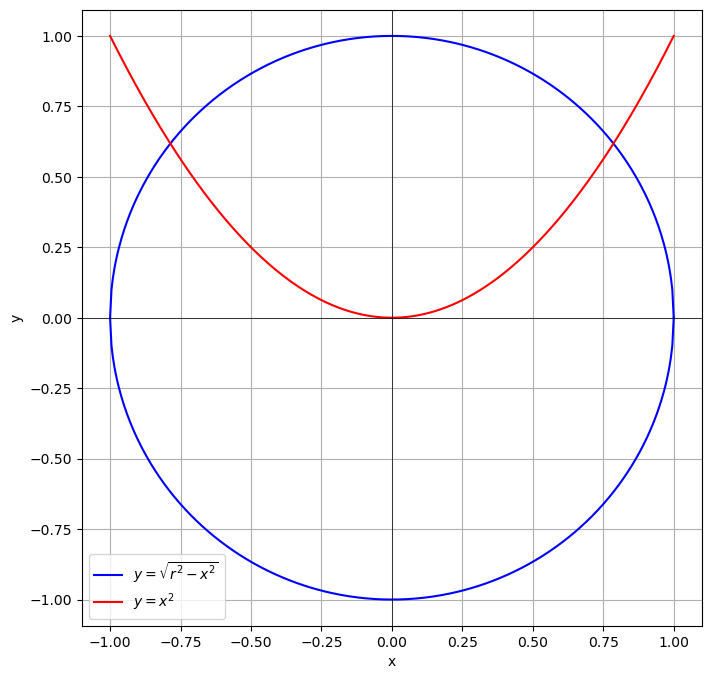
\includegraphics[width = 0.75\linewidth]{function&relation.png}
    \caption{Visual Comparison of a Relation and a Function}
\end{figure}
\begin{example}
	Let A be the set {1,2,3,4}. Which ordered pairs are in the relation $R=\{(a,b)\mid a$ divides $b\}?$
	\begin{solution}
		 Because $(a,b)$ is in R if and only if $a$ and $b$ are positive integers not exceeding 4 such that $a$ divides $b$,we see that
		$$
		R=\{(1,1),(1,2),(1,3),(1,4),(2,2),(2,4),(3,3),(4,4)\}.
		$$
	\end{solution}
\begin{figure}[H]
	\centering
\begin{tikzpicture}
	
	% Define style for the nodes
	\tikzstyle{number}=[circle, draw, inner sep=2pt]
	
	% Draw nodes
	\node[number] (1l) at (0,3) {1};
	\node[number] (2l) at (0,2) {2};
	\node[number] (3l) at (0,1) {3};
	\node[number] (4l) at (0,0) {4};
	
	\node[number] (1r) at (2,3) {1};
	\node[number] (2r) at (2,2) {2};
	\node[number] (3r) at (2,1) {3};
	\node[number] (4r) at (2,0) {4};
	
	% Draw arrows
	\draw[->] (1l) -- (1r);
	\draw[->] (1l) -- (2r);
	\draw[->] (1l) -- (3r);
	\draw[->] (1l) -- (4r);
	
	\draw[->] (2l) -- (2r);
	\draw[->] (2l) -- (4r);
	
	\draw[->] (3l) -- (3r);
	
	\draw[->] (4l) -- (4r);
\end{tikzpicture}
\caption{$R=\{(a,b)\mid a$ divides $b\}$}
\end{figure}
This relation also differs from function, since for member of $a$, it is possible
to map to multiple members in $b$.
\end{example}
\begin{definition}[Functional Relation]
    A relation $R$ is said to be \textbf{functional} if each element of its domain has exactly one $R$-relative; 
    a functional relation is also called a \textbf{function}. If $R$ is a functional relation then for each element 
    $a$ of its domain we denote the unique $R$-relative of $a$ by $R(a).$ 
\end{definition}

    This leads us to the next axiom of NBG theory.
    \begin{axiom}[Replacement Axiom]
        For every functional relation $R$, if the domain of $R$ is a set then the range 
        of $R$ is also a set.
    \end{axiom}

    In naive set theory and function in part 1 of the book, we gave a rough 
    definitions to mappings. With class, we can make it more concrete.
    \begin{definition}[mapping]
        A mapping is an ordered pair $((A,B),R)$ where $A$ and $B$ are sets and $R$ is a 
        functional relation between $A$ and $B$ such that Dom $R=A.$ If 
        $f= ( ( A, B) , R) $ is a mapping we say that $f$ is a mapping from 
        $A$ to $B;$ we call $A$ the domain of $f,B$ the codomain of $f$ and $R$ the 
        graph of $f$. If $f$ is a mapping with domain $A$ and codomain $B$ we often write $f:A\to B.$ 
        If $a$ is any element of the set $A$ then the set $R^{\to}(\{a\})$ consists of a single element of 
        $B$ which we denote by $f(a);$ we call it the image of $a\textbf{ under }f$ or the value of $f\textbf{ at }a.$
    \end{definition} 
    It is clear from the definition of the term “mapping” that in order to describe a mapping $f$ we must give the domain $A$ and codomain $B$ of $f$ and also, for each element $a$ of the domain we must describe the unique element $b_a$ of the codomain such that $(a,b_a)$ belongs to the graph of $f$, i.e. we must describe for each element $a$ of $A$ its image under $f$ in $B.$
    Let $f= ( ( A, B) , R) $ be a mapping from $A$ to $B$. For each subset $X$ of $A$ we denote the subset 
    $R^{\to}(X)$ of $B$ by $f^{\to}(X);$ in particular, if $a$ is any element of $A$ we have
    $f^{\to}(\{a\})=\{f(a)\}.$ For each subset $Y$ of $B$ we denote the subset $R^{\leftarrow }( Y) $ 
    of $A$ by $f^{\leftarrow }( Y) .$

    Let $ f=((A,B),R)$ be a mapping from $A$ to $B;\operatorname*{let}A_1$ be a subset of $A.$ Then the restriction of $f$ to $A_1$ is the mapping $f\mid A_1=$
    $$
    ((A_1,B),R\cap(A_1\times B)).
    $$

    Earlier, we discussed composition and inverse of function. Now that we have known that function is a kind of 
    relation, can we compose or inverse all other relations? Naturally the answer is yes.

    \begin{definition}[Composite Relation]
        If $R$ and $S$ are relations, the composition of $R$ and $S$ is the relation $S\circ R$ given by
        $$
        S\circ R=\{(x,z):(\exists y)(((x,y)\in R)\wedge((y,z)\in S))\}.
        $$
        If $R$ is a relation between $A$ and $B$ and $S$ is a relation between $B$ and $C$ then clearly 
        $S\circ R$ is a relation between $A$ and $C$, and we have $\operatorname{Dom}\left(S\circ R\right)\subseteq\operatorname{Dom}R$ and Range $(S\circ R)\subseteq\operatorname{Range}S.$
    \end{definition}
    The idea of composition also works for mappings.
\begin{definition}[Composite Mapping]
    Let $f= ( ( A, B) , R) $ and $g= ( ( B, C) , S) $ be mappings. Then clearly 
    $((A,C),S\circ R)$ is also a mapping, which we denote by $g\circ f$ and call the composition or 
    composed mapping of $f$ and $g$. For each element $a$ of $A$ we have $( g\circ f) ( a) = g( f( a) ).$

\end{definition}
\begin{remark}
	The other equivalent definition is that
	Let $R$ be a relation from a set $A$ to a set $B$ and S a relation from $B$ to a set $C$. The $composite$ of $R$ and S is the relation consisting of ordered pairs $(a,c)$, where $a\in A, c\in C$ , and for which there exists an element $b\in B$ such that $( a, b) \in R$ and $( b, c) \in S.$ We denote the composite of $R$ and $S$ by $S\circ R.$
\end{remark}
    Similarly, we can define inverse relation.
    \begin{definition}[Inverse Relation]
        If $A$ and $B$ are classes then a relation between $A\textbf{ and }B$ is a subclass of $A\times B$, 
        i.e. a relation $R$ such that Dom $R\subseteq A$ and Range $R\subseteq B.$ A relation on a class $A$ 
        is a subclass of $A\times A.$

        If $R$ is a relation, the inverse of $R$ is the relation $R^{-1}$ given by
        $$
        R^{-1}=\{(x,y):(y,x)\in R\}.
        $$
        If $R$ is a relation between $A$ and $B$ then $R^{-1}$ is a relation between $B$ and $A;$ 
        clearly Dom $R^{-1}=\operatorname{Range}R$ and Range $R^{-1}=\operatorname{Dom}R.$
    \end{definition}

    Let $R$ be a relation, $A$ any class. Then the image of $A\textbf{ under }R$ is the class consisting of all $R$-relatives of all members of $A.$ We denote this class by $R^{\to}(A).$ Thus
    $$
    R^{\to}(A)=\{y:(\exists x)((x\in A)\land((x,y)\in R))\}.
    $$
    Again let $R$ be a relation and $\ker B$ be any class. Then the inverse image of $B$ under $R$ is the class $( R^{- 1}) ^{\to }( B) , $ which we write $R^{\leftarrow}( B) .$ Thus
    $$
    \begin{aligned}R^{\leftarrow}(B)=\{x:(\exists y)((y\in B)\land((x,y)\in R))\}.\end{aligned}
    $$
    With functional relation and mapping, we can define a more specific relation, which very special and practical.
    \begin{definition}[Diagonal (Relation) and Identity Mapping]
    	Let $A$ be any set; let $D_A=\{x:(\exists a)((a\in A)\land(x=(a,a)))\}$ (we call $D_A$ the diagonal of $A\times A).$ Then $D_A$ is a functional relation between $A$ and $A$ with domain $A.$ The mapping $I_A=((A,A),D_A)$ from $A$ to $A$ is called the identity mapping of $A.$ Clearly we have $I_{A}(a)=a$ for each element $a$ of $A.$
    \end{definition}
   \begin{example}
   	The identity mapping $I_A$ for a set $A$ is a function that maps every element to itself. Here are some examples of identity mappings on various sets:
   	
   	\begin{itemize}
   		\item Let $B = \{x \in \mathbb{R} \mid -1 \leq x \leq 1\}$. The identity mapping on $B$ is $I_B : B \to B$ where $I_B(x) = x$ for all $x \in B$.
   		
   		\item Let $C = \{\text{apple}, \text{banana}, \text{cherry}\}$. The identity mapping on $C$ is $I_C : C \to C$ where $I_C(\text{fruit}) = \text{fruit}$ for each fruit in set $C$.
   		
   		\item Let $D = \mathbb{Z}$. The identity mapping on $D$ is $I_D : \mathbb{Z} \to \mathbb{Z}$ where $I_D(n) = n$ for all $n \in \mathbb{Z}$.
   	\end{itemize}
   	
   	The diagonal for each of these sets would be as follows:
   	\begin{itemize}
   		\item The diagonal of $B$, $D_B$, would be the set of all ordered pairs $(x, x)$ such that $x \in B$.
   		
   		\item The diagonal of $C$, $D_C$, would be the set $\{(\text{apple}, \text{apple}), (\text{banana}, \text{banana}), (\text{cherry}, \text{cherry})\}$.
   		
   		\item The diagonal of $D$, $D_D$, would be the set of all ordered pairs $(n, n)$ such that $n \in \mathbb{Z}$.
   	\end{itemize}
   	
   	In all these cases, the identity mapping illustrates the concept of a function where the input is the same as the output for each element of the set.
   \end{example}
\subsubsection*{Families of Sets}
In part 1, we discussed sequence. Sequence is defined (see definition \ref{def_sequence}) by a relation between index and a mathematical expression related to the index, and commonly the index $i$ has $i\in \N$. Sequence is actually a special \textbf{family of set}.
\begin{definition}[Family of Set]
	Let $I$ and $A$ be classes, and $F$ is a functional relation between $I$ and $A$. Then $F$ is sometimes called a family of elements of $A$ indexed by $I$ (or with $I\textbf{ as index class}) $ and we write $(F(i))_{i\in I}$ instead of $F$. In particular, if $E$ is a set then a family of elements of $\mathbf{P}(E)$ is called a family of subsets of $E$ indexed by $I.$ If $F$ is such a family and we write $X_i=F(i)$ for each element $i$ in $I$ then we denote the family $F$ by$\left ( X_i\right ) _i\in I.$
\end{definition} 
If $X$ is a set of subsets of a set $E$ then the diagonal $D_X$ is a family of subsets of $E$ which may sometimes be denoted by $(x)_{x\in X}.$

Let $F= ( X_{i}) _{i\in I}$ be a family of subsets of a set $E.$ We define the union of the family to be
$$
\bigcup_{i\in I}X_i=\{x:(\exists i)((i\in I)\land(x\in X_i))\}.
$$
Thus $x$ belongs to the union of the family $(X_i)_{i\in I}$ if and only if it belongs to at least one of the sets $X_i$ with $i$ in $I.$ Of course if $X$ is a set of subsets of $E$ the union of the corresponding family $D_X$ coincides with the union of the set $X$ as previously defined: $\left(\bigcup_{x\in X}x=\left(\right.\right)X.$

Again let $(X_i)_{i\in I}$ be a family of subsets of a set $E.$ The intersection of this family is defined to be
$$
\bigcap_{i\in I}X_i=\{x:(x\in E)\land(\forall i)((i\in I)\Longrightarrow(x\in X_i))\}.
$$
So $x$ belongs to the intersection of the family $(X_i)_{i\in I}$ if and only if it belongs to all the sets $X_i$ with $i$ in $I.$

We notice that if $I$ is empty then we have $\bigcap_{i\in I}X_i=E.$ If X i a non-empty set of subsets of $E$ the intersection of the corresponding family $D_X$ coincides with the intersection of the set $X$ as previously defined${: }\bigcap _{x\in X}x= \bigcap X.$


\begin{definition}[Sequence as Family of Set]
A sequence in a set \( X \) can be defined as a function \( s: \mathbb{N} \to X \), where \( \mathbb{N} \) denotes the set of natural numbers. For each \( n \in \mathbb{N} \), the element \( s(n) \) is referred to as the \( n \)-th element of the sequence. The sequence is often denoted by \( (a_n)_{n \in \mathbb{N}} \), which signifies a family of elements \( a_n \) indexed by \( n \).
\end{definition}
\subsection{Reflexivity, Symmetry, and Transitivity}
\subsection{Anti-symmetry and Asymmetry}
\subsection{Representation of Relation}
\subsection{Exercises}
\begin{exercise}
	 Determine whether each of the following is a set or a class in NBG set theory, and explain why.
	\begin{enumerate}
		\item The collection of all sets that do not contain themselves.
		\item The set of all natural numbers.
		\item The class of all ordinal numbers.
	\end{enumerate}
\end{exercise}
\begin{solution}
	Below are the solutions.
	\begin{enumerate}
		\item The collection of all sets that do not contain themselves is a \textbf{proper class}. This is because any attempt to consider it as a set leads to Russell's paradox, thus it cannot be a set within any consistent set theory including NBG.
		\item The set of all natural numbers is a \textbf{set}. It is well-defined and does not lead to any paradoxes within NBG set theory. Furthermore, it is an element of the class of all sets.
		\item The class of all ordinal numbers is a \textbf{proper class} because it is too large to be a set. If it were a set, it would lead to contradictions similar to those arising from considering the "set of all sets."
	\end{enumerate}
\end{solution}
\begin{exercise}
    Russel's Paradox is fixed by introducing more strict set axioms to the set theory. In NBG theory, a
    proper class is defined as a top-level class that cannot be subclass of any other classes or sets, and
    this is the key to avoid the paradox in naive set theory. Explain in details that how 
    this concept avoids the case in Russel's Paradox.
\end{exercise}
\begin{solution}
    With the introduction of the concept of classes, we can discuss collections 
    that are too large to be considered as sets, such as the ``class of all sets.'' 
    Therefore, the set described by Russell's Paradox, denoted by \( R \), 
    is no longer considered a legitimate set but rather a ``proper class.'' 
    This means that we refrain from discussing \( R \) as a set, thereby avoiding 
    the paradox because proper classes are not subject to the operations and 
    axioms that constrain sets. As a result, the axiomatic system does not 
    permit the formation of sets that would lead to Russell's Paradox.

\end{solution}
\begin{exercise}
    Let $A,B,C$ be classes such that $A\subseteq B,B\subseteq C$, $C\subseteq A.$ Prove that $A=B=C.$
\end{exercise}

\begin{exercise}
    Let $A,B,C$ be classes such that $A\subset B,B\subset C.$ Prove that $A\subset C.$
\end{exercise}


\section{Equivalence Relations}



\subsection{Exercises}
\section{Partial and Total Order Relations}



\subsection{Exercises}
\section{Special Types of Relations}
\subsection{Recursive Relations}
\subsection{\(n\)-ary Relations}

\subsection{Exercises}



\begin{comment}
    

\section{Searching algorithms}
    The very first thing we need to do is figure out what is searching, before we do any math.
    \begin{definition}[Searching algorithm]
        Given an array \( A[1], A[2], A[3], \ldots, A[n] \) and a target value \( T \), find an index \( j \) where \( T = A[j] \) or determine that no such index exists because \( T \) is not in the array \( A \).
    \end{definition}
    \subsection{Searching in Unordered Array List}
    We proceed to analyze the most common case, where we need to find the element $T$ from an unordered 
    array. In this case, what we need to do is just like counting numbers. We will check each element in
    the array $A$, from $A[1]$ to $A[n]$, until we find $T$. This way of reaching in pure sequential 
    order is called \textbf{Linear Search}. The pseudocode is shown below.
    \begin{algorithm}
        \caption{Linear search for a target value in an array}
        \begin{algorithmic}[1]
        \Procedure{LinearSearch}{$A, T$}
            \For{$j = 1$ to $j=n$}
                \If{$A[j] == T$}
                    \State \Return $j$
                \EndIf
            \EndFor
            \State \Return $\text{``not found''}$
        \EndProcedure
        \end{algorithmic}
        \end{algorithm} 
    This is the easiest  algorithm in this book, and it is clear that for an array of size $n$, this 
    algorithm has a time complexity of $O(n)$ in the worst cases. Now consider that, what if we are lucky
    enough to find our target $T$ in the very first element in the array? Actually, computer scientists
    have the other notation to show the best-case performance of a algorithm, which is $\omega$ notation.
    \begin{notation}[Omega Notation]
        The Omega notation describes the lower bound of an algorithm's running time. 
        It measures the best-case scenario, at least this fast. For a given function g(n), 
        we denote $\omega(g(n))$ the set of functions:
        \[
        \Omega(g(n)) = \{ f(n) : \exists c > 0, n_0 > 0 \text{ such that } 0 \leq cg(n) \leq f(n) \text{ for all } n \geq n_0 \}
        \]
    \end{notation}
    Yet there is another notation to show the overall, or average performance of an algorithm.
    \begin{notation}[Theta Notation]
        The Theta notation tightly bounds a function from above and below, meaning it defines an algorithm's running time both in the best and worst cases. For a given function $g(n)$, we denote $\Theta(g(n))$ the set of functions:
        \[
        \Theta(g(n)) = \{ f(n) : \exists c_1 > 0, c_2 > 0, n_0 > 0 \text{ such that } 0 \leq c_1g(n) \leq f(n) \leq c_2g(n) \text{ for all } n \geq n_0 \}
        \]
    \end{notation}
    Theta notation is used to evaluate the average time complexity of executing an algorithm. For instance,
    we use $\bar{p}$ to denote the average of accessed elements. We have:
    $$\bar{p} = \frac{1}{n} \sum_{i=i}^{n}i = \frac{1}{n}\times\frac{n(n+1)}{2}=\frac{n+1}{2}$$
    Which means this algorithm has $\Theta(\frac{n+1}{2})$ time complexity.
    \subsection{Searching in Ordered Array List}
    It seems that we do not have any better way to design a more efficient algorithm for finding target in 
    unordered array. Now we will discuss the case for an ordered array.
    \begin{definition}
        An ordered array refers to an array $A$ that satisfies $A[1]\leq \cdots \leq A[n]$ or $A[1]\geq 
        \cdots, \geq A[n]$.
    \end{definition}
    In this case, the target $T$ and any random element $A[n]$ in the array has the following properties
    \begin{itemize}
        \item  If \( T < A[i] \), then \( T \) cannot occur among \( A[i], A[i + 1], \ldots, A[n] \), and we need only search the list from \( A[1] \) to \( A[i - 1] \)
        \item  If \( A[i] < T \), then \( T \) cannot occur among \( A[1], A[2], \ldots, A[i] \), and we need only search the list from \( A[i + 1] \) to \( A[n] \)
    \end{itemize}
    If we adopt a policy of making the worst case as favorable as we can, we should
    probe in the middle (or as near to the middle as possible) of the list (or sublist) we're
    searching. Then, if we don't find the target there, we will have at most half the list to
    search.
    
    Suppose the partition of the original list we are searching in is from $A[p]$ to $A[q]$. We can get
    the median by $\frac{p+q}{2}$, however, when $p+q$ is odd, we cannot get a valid integer as position
    of element. As a result, we probe $A[i]$ where $i = \lfloor \frac{p+q}{2} \rfloor$ instead. 
    The resulting search algorithm where we probe in the middle of the current
    sublist is \textbf{Binary Search}.
    \begin{algorithm}[H]
        \caption{Binary Search for a target value in a sorted array}
        \begin{algorithmic}[1]
        \Procedure{BinarySearch}{$A, T$}
            \State $p \gets 1$
            \State $q \gets n$
            \While{$p \leq q$}
                \State $j \gets \left\lfloor (p + q) / 2 \right\rfloor$
                \If{$A[j] == T$}
                    \State \Return $j$
                \ElsIf{$A[j] < T$}
                    \State $p \gets j + 1$
                \Else
                    \State $q \gets j - 1$
                \EndIf
            \EndWhile
            \State \Return $\text{``not found''}$
        \EndProcedure
        \end{algorithmic}
        \end{algorithm}
    \begin{remark}
        If this code is a little confusing for you, you may check \href{https://www.cs.usfca.edu/~galles/visualization/Search.html}{here}
        for complete visualization of binary search.
    \end{remark}
    
    Walkthrough with $n = 12$ and $A = (3, 5, 8, 8, 9, 16, 29, 41, 50, 63, 64, 67)$. 

    If $T=99$, then, we can show the variables involved in a table.
    \begin{table}[h!] 
        \label{bisearch1}
        \centering
        \begin{tabular}{cccccc}
        \toprule
        \( p \) & \( j \) & \( q \) & \( A[j] \) & relation     & output         \\
        \midrule
        1       & 6       & 12      & 16         & \( A[j] < T \) & -             \\
        7       & 9       & 12      & 50         & \( A[j] < T \) & -             \\
        10      & 11      & 12      & 64         & \( A[j] < T \) & -             \\
        12      & 12      & 12      & 67         & \( A[j] < T \) & -             \\
        13      & -       & 12      & -          & -              & \( T \) is not in \( A \) \\
        \bottomrule
        \end{tabular}
        \caption{Binary Search Iterations}
        \end{table}
        Suppose the sublist we're searching is from \( A[p] \) up to \( A[q] \) of length \( k = q - p + 1\) and we probe unsuccessfully at \( A[j] \):
        $$\underbrace{A[p]\ldots A[j-1]}_{k1}\quad\text{A}[j]\quad\underbrace{A[j+1]\ldots A[q]}_{k2}$$
        
        If \( A[j] \geq T \), then we will search from \( A[p] \) up to \( A[j-1] \) of length \( k_1 = j - p \). \\
        
        If \( A[j] < T \), then we will search from \( A[j+1] \) up to \( A[q] \) of length \( k_2 = q - j \). \\
        
        We would like \( k_1 \) and \( k_2 \) to be equal, but if that's not possible (because \( q - p \) is odd), let's consistently make \( k_1 \) the smaller value.
        $\text{How should we choose }  j  \text{ so that }  k_1 \leq k_2  \text{ and }  k_2$  is as small as possible?
        To make \( k_2 = q - j \) as small as possible, we need to make \( j \) as large as possible. We want
        
        \[ k_1 + k_2 \leq k_2 + k_2, \]
        that is,
        \[ q - p \leq 2(q - j) = 2q - 2j \]
        or
        \[ 2j \leq 2q - (q - p) = q + p. \]
        
        The largest integer \( j \) such that \( j \leq (q + p)/2 \) is \( \lfloor (q + p)/2 \rfloor \), and this is the \( j \)-value used in the algorithm.
        \begin{theorem}[Binary Search Sublist Lengths] \label{sublistlen}
            On each iteration of Binary Search with \( j = \left\lfloor \frac{p + q}{2} \right\rfloor \), the lengths of the sublists will be \( k_1 = \left\lfloor \frac{k - 1}{2} \right\rfloor \) such that \( k_1 \leq k_2 = \left\lceil \frac{k - 1}{2} \right\rceil \leq \frac{k}{2} \).
            \end{theorem}
            
            \begin{proof}
            Since \( j \leq \frac{q + p}{2} < j + 1 \), subtracting \( p \) from each of these three expressions gives
            \begin{align*}
            j - p &\leq \frac{q + p}{2} - p < j - p + 1 \\
            k_1 &\leq \frac{q - p}{2} < k_1 + 1.
            \end{align*}
            Thus, \( k_1 = \left\lfloor \frac{q - p}{2} \right\rfloor = \left\lfloor \frac{k - 1}{2} \right\rfloor \).
            
            Because \( k_1 + k_2 = k - 1 \), we know that
            \begin{itemize}
            \item if \( k \) is odd, say \( k = 2r + 1 \), then \( k - 1 = 2r \) and \( k_1 = r = k_2 < \frac{k}{2} \),
            \item if \( k \) is even, say \( k = 2r \), then \( k - 1 = 2r - 1 \) and \( k_1 = r - 1 < r = k_2 = \frac{k}{2} \).
            \end{itemize}
            Thus, \( k_1 = \left\lfloor \frac{k - 1}{2} \right\rfloor \leq k_2 = \left\lceil \frac{k - 1}{2} \right\rceil \leq \frac{k}{2} \).
            \end{proof}

            \begin{theorem}[Binary Search Termination]
                Binary Search terminates after at most \(\lceil \lg(n) \rceil + 1\) probes.
                \end{theorem}
                
                \begin{proof}
                Let \( w = \lfloor \lg(n) \rfloor \). If, in some instance, Binary Search has not terminated after \( w \) (unsuccessful) probes, then the current value of \( p \) must be \( \leq \) the current value of \( q \), and the length of the current sublist, \( k \), must be \( \leq n/2^w \).
                \[ // \text{Prove this by MI.} \]
                Since \( w \leq \lg(n) < w + 1 \),
                \[ 2^w \leq n < 2 \times 2^w \]
                \[ // \text{then dividing each by } 2^w \]
                \[ 1 \leq n/2^w < 2. \]
                \[ // \text{which implies that } k = 1 \]
                
                For the next iteration, \( p = q \) and so \( j = p \).
                \[ // \text{And we probe the one remaining entry in } A. \]
                
                If \( A[j] < T \), then \( p \leftarrow j + 1 > q \), so Binary Search terminates after this probe; if \( A[j] > T \), then \( q \leftarrow j - 1 < p \), so Binary Search terminates after this probe; and if \( A[j] = T \), then Binary Search terminates after this one last probe.
                
                Therefore, Binary Search terminates after at most \(\lceil \lg(n) \rceil + 1\) probes.
                \end{proof}
    To show that the binary search algorithm is correct, we also need to show its \textbf{loop invariant}.
        \begin{definition}
            In computer science, a loop invariant is a logical assertion that is true before and after 
            each iteration of a program loop. It is a condition that is true at the beginning and 
            end of every iteration of a loop.
        \end{definition}
    Assume that $T$ is in $A$ and $T=A[i]$, $i \in [p, q]$.
    \begin{theorem}[Loop Invariance of Binary Search]
        After $k$ iterations of the loop, if $T$ = $A[i]$, then $p\leq i \leq q$.
    \end{theorem}
    \begin{proof}
        By Mathematical Induction on \(k\) where \(k \in \{0..\}\)

\textbf{Step 1.} After \(k = 0\) iterations of the loop, that is, before the loop is done once
\[ p = 1 \quad \text{and} \quad q = n, \]
and therefore,
\[ \text{if} \quad T = A[i] \quad \text{then} \quad p \leq i \leq q. \quad (\text{P}(0) \text{ is True}) \]

\textbf{Step 2.} Assume \(\exists w \in \mathbb{N}\) such that
after \(w\) iterations of the loop, if \( T = A[i] \), then \( p \leq i \leq q \). \quad (\text{This is P}(w).)

\textbf{Step 3.} Suppose there is another iteration, the \( w + 1^{st} \).
That is, \( T \) has not been found in \( w \) unsuccessful probes, and now, \( p \leq q \).
On the next iteration, we calculate a new \( j \)-value,
\[ j_{\text{new}} \leftarrow \left\lfloor \frac{(p + q)}{2} \right\rfloor \]

Since \( p \leq q \),
\[ p + p \leq p + q \leq q + q \]
and
$$p\ =\ \frac{p+p}{2} \leq \frac{p+q}{2} \leq \frac{q+q}{2} =q$$
and so \( p \leq j_{\text{new}} \leq q \).
In fact, if \( p = q \), then \( j_{\text{new}} = p \), and if \( p < q \), then \( p \leq j_{\text{new}} < q \).

In the remainder of the proof, we will let \( p^* \) and \( q^* \) denote the values of \( p \) and \( q \) at the end of the iteration. There are three cases to consider:

\textbf{Case 1.} If \( A[j_{\text{new}}] < T \), then \( T \) cannot occur at or before position \( j_{\text{new}} \) hence
\[ \text{if} \quad T = A[i] \quad \text{then} \quad p < j_{\text{new}} + 1 \leq i \leq q. \quad \text{Here} \quad p^* = j_{\text{new}} + 1 \quad \text{and} \quad q^* = q. \]

\textbf{Case 2.} If \( A[j_{\text{new}}] > T \), then \( T \) cannot occur at or after position \( j_{\text{new}} \) hence
\[ \text{if} \quad T = A[i] \quad \text{then} \quad p \leq i < j_{\text{new}} - 1 < q. \quad \text{Here} \quad p^* = p \quad \text{and} \quad q^* = j_{\text{new}} - 1. \]

\textbf{Case 3.} If \( A[j_{\text{new}}] = T \), then neither \( p \) nor \( q \) are changed hence, from Step 2
\[ \text{if} \quad T = A[i] \quad \text{then} \quad p \leq i \leq q. \quad \text{In this case,} \quad p^* = p \quad \text{and} \quad q^* = q. \]

Therefore, after this next iteration,
\[ \text{if} \quad T = A[i] \quad \text{then} \quad p^* \leq i \leq q^*. \quad \text{in every case} \]
    \end{proof}
    \begin{remark}
    When the repeat-loop in Binary Search terminates,
    \[ \text{if} \quad T = A[i], \quad \text{then} \quad p \leq i \leq q. \quad \text{(That is, this conditional statement is True.)} \]
    
    But if \( p > q \), there is no index \( i \) where \( p \leq i \leq q \).
    \[ \text{(The consequent must be False. The antecedent must be False.)} \]
    
    If \( p > q \), there is no index \( i \) where \( T = A[i] \).
    \[ \text{(If \( p > q \), then \( T \) cannot be in \( A \). Therefore, when Binary Search terminates,} \]
    
    the target has been found at position \( j \)
    or
    \[ (p > q \quad \text{and so} \quad T \text{ is not in } A.) \]
    
    Binary Search is correct and very efficient.
    \[ \text{(compared to Linear Search)} \]
    \end{remark}

    \subsection*{Branching Diagrams}
    \begin{definition}[Branching Diagram]
        A General Branching Diagram for an algorithm is a tree that shows all possible
        sequences of operations the algorithm might do.
    \end{definition}
    Branching tree is an important tool for algorithm analysis; when n is not very large, we can draw the
    branching diagram for algorithm analysis.

    Suppose that we have an array with $n=12$. In this branching tree, each cell represent a result of iterating element in the array. Certainly, we have $A[6]$ as the first element to be accessed.
    With 6 visited, there are two possible consequence of comparisons which will lead us to either
    $A[3]$ or $A[9]$, and so forth.
    \begin{figure}[H]
        \centering
        \includegraphics[width = 0.8 \textwidth]{"branchingtree.png"}
        \caption{Branching Tree of Binary Search}
    \end{figure}

    This kind of diagram is known as a \textbf{Binary Tree}: it's “rooted” at the vertex
    placed at the top of the diagram, and is binary in the sense that from any vertex,
    there are at most two edges downward in the diagram. The vertices with no
    downward edges are called \textbf{leaves}. The other vertices are called \textbf{internal vertices}.
    Every vertex, except the root, is the end of exactly one edge to it from a vertex
    above it in the diagram.

    \subsection{Binary Search: Version 2}
    Now we look into the other version of binary search.
    \begin{algorithm}[H]
        \caption{Binary Search Version 2 for a target value in a sorted array}
        \begin{algorithmic}[1]
        \Procedure{BinarySearch}{$A, T$}
            \State $p \gets 1$
            \State $q \gets n$
            \While{$p < q$}
                \State $j \gets \left\lfloor (p + q) / 2 \right\rfloor$
                \If{$A[j] < T$}
                    \State $p \gets j + 1$
                \Else
                    \State $q \gets j$
                \EndIf
            \EndWhile
            \If{$A[p] = T$}
                \State \Return $p$
            \Else
                \State \Return \textit{not found}
            \EndIf
        \EndProcedure
        \end{algorithmic}
        \end{algorithm}
    There is only one major difference between these 2 versions. For $p$ and $q$, the way they are updated in
    the second version is different, as $q$ is assigned by $j$ instead of $j-1$. It seems that this is 
    only a trivial change in the algorithm, mathematically, however, it changes the way how it works completely.
    We refer to the same example where $T=99$.
    \begin{table}[h!]
        \centering
        \caption{Execution steps of Binary Search when $T = 99$}
        \begin{tabular}{ccccccc}
        \toprule
        $p$ & $j$ & $q$ & $p < q$ & $A[j]$ & $A[j] < T$ & Output \\
        \midrule
        1 & 6 & 12 & t & 16 & t & - \\
        7 & 9 & 12 & t & 50 & t & - \\
        10 & 11 & 12 & t & 64 & t & - \\
        12 & - & 12 & f & - & - & $T$ is not in $A$ \\
        \bottomrule
        \end{tabular}
    \end{table}

    Comparing with the table \ref{bisearch1}, the number of iteration decreases by 1.

    Is this algorithm really correct? To figure it out, recall that to show an algorithm correct,
    we need to secure its loop invariance and whether it is terminable. Actually, this algorithm 
    operates on two partitions of the array only, but not 3, as in the previous version. 
    Suppose the sublist we're searching is from $A[p]$ up to $A[q]$ of length $k = q-p+1$, and we
    make the comparison “is $A[j] < T$?”:
    $$\underbrace{A[p] \ldots A[j]}_{k 1} \quad \underbrace{A[j+1] \ldots A[q]}_{k 2}$$

    In this case, $A[j]$ is not considered as an independent element, but the last element of sublist $p$ to $j$.
    If $A[j] < T$, the Procedure will try to find it in $k2$ by assign the index of the smallest item in it 
    to $p$. And if $A[j] \geq T$, it is just the other way around. Recall that in theorem \ref{sublistlen},
    when $j = \lfloor \frac{p+q}{2}\rfloor$ the length of $k1$  will be $\lfloor\frac{k-1}{2}\rfloor$, 
    while length of $k2$ is $\lceil \frac{k-1}{2}\rceil$. However, $\forall k\in \mathbb{Z}$, 
    $\lceil \frac{k-1}{2} \rceil = \lfloor \frac{k}{2}\rfloor$ (proven in previous chapter).

    Since $k_1 + k_2 = k$, we have
    \[
    \text{if } k \text{ is even, say } k = 2r, \text{ then } k_1 = r = k_2 = \frac{k}{2} \text{ and}
    \]
    \[
    \text{if } k \text{ is odd, say } k = 2r + 1, \text{ then } k_2 = r < \frac{k}{2} < r + 1 = k_1.
    \]
    In general,
    \[
    k_2 = \left\lfloor \frac{k}{2} \right\rfloor \leq \frac{k}{2} \leq k_1 = \left\lceil \frac{k}{2} \right\rceil.
    \]

    Therefore, at some iterations of binary search \#2, the length of the next sublist is more than half the length of the previous sublist.

    Let $L(w)$ denote the length of the sublist still to be searched after $w$ iterations of the while loop.
    \begin{theorem}\label{4.2.1}
        After $w$ iterations of the loop
        \[
        \left\lfloor \frac{n}{2^w} \right\rfloor \leq L(w) \leq \left\lceil \frac{n}{2^w} \right\rceil.
        \]
    \end{theorem}
    \begin{proof}
        Denote the statement as $P(w)$

        By Mathematical Induction on $w$ where $w \in \{0, \ldots\}$.

    \paragraph{Step 1.}
        After $w = 0$ iterations of the loop, before the loop is done once the length of the current sublist,
        \[
        L(0) = n = \left\lceil \frac{n}{2^0} \right\rceil = \left\lfloor \frac{n}{2^0} \right\rfloor.
        \]
        $P(0)$ is True.

        Suppose that for the first few iterations of the loop (even though $p$ and $q$ may have been changed), these bounds on the length of the current sublist are maintained.

        \paragraph{Step 2.}
        Assume there exists $m \in \mathbb{N}$ such that after $m$ iterations of the loop
        \[
        \left\lfloor \frac{n}{2^m} \right\rfloor \leq L(m) \leq \left\lceil \frac{n}{2^m} \right\rceil.
        \]
        This is $P(m)$.

        \paragraph{Step 3.}
        Suppose there is another iteration, the $m + 1$. That is, now $p < q$. We know that
        \[
        \left\lfloor \frac{L(m)}{2} \right\rfloor \leq L(m + 1) \leq \left\lceil \frac{L(m)}{2} \right\rceil.
        \]
        If we can show that
        \[
        \lceil L(m) / 2\rceil\leq\left\lceil\left\lceil n / 2^{m}\right\rceil / 2\right\rceil \text { and }\left\lceil\left\lceil n / 2^{m}\right\rceil / 2\right\rceil \leq \left\lceil n / 2^{m+1}\right\rceil
        \]
        we will have the upper bound we want: $L(m + 1) \leq \left\lceil \frac{n}{2^{m+1}} \right\rceil$.

        We deal with these (and the corresponding inequalities with the floor function) in a more general setting in the next two lemmas.

        Remember that $\left\lceil r \right\rceil$ is (defined to be) the smallest integer greater than or equal 
        to the (real) number $r$ and $\left\lfloor r \right\rfloor$ is the largest integer less than or equal 
        to $r$. Also, recall that whenever $y$ is not an integer, $\left\lfloor y \right\rfloor < y < \left\lfloor y \right\rfloor + 1$.
        
        It takes some extra step to show this. We will prove the inductive hypothesis by 2 lemmas.

        \noindent \textbf{Lemma 1}: If \( x \) and \( y \) are real numbers and \( x < y \), then \( \lceil x \rceil \leq \lceil y \rceil \) and \( \lfloor x \rfloor \leq \lfloor y \rfloor \).
        \begin{proof}
            The floor and ceiling functions are nondecreasing.
            Since \( x < y \leq \lceil y \rceil \in \mathbb{Z} \) and \( \lceil x \rceil \) is the smallest integer \( \geq x \), \( \lceil x \rceil \leq \lceil y \rceil \).
            Since \( \lfloor x \rfloor \leq x < y \) and \( \lfloor y \rfloor \) is the largest integer \( \leq y \), \( \lfloor y \rfloor \geq \lfloor x \rfloor \).
        \end{proof}

        \noindent \textbf{Lemma 2}: For any real number \(x\), \(\left\lfloor \frac{\lfloor x\rfloor}{2} \right\rfloor = \left\lfloor \frac{x}{2} \right\rfloor\) and \(\left\lceil \frac{\lceil x\rceil}{2} \right\rceil = \left\lceil \frac{x}{2} \right\rceil\).
        \begin{proof}
            If \(x\) is an integer, then \(\lfloor x\rfloor = x = \lceil x\rceil\), and therefore,
            \[
            \left\lfloor \frac{\lfloor x\rfloor}{2} \right\rfloor = \left\lfloor \frac{x}{2} \right\rfloor
            \]
            and
            \[
            \left\lceil \frac{\lceil x\rceil}{2} \right\rceil = \left\lceil \frac{x}{2} \right\rceil
            \].
            Suppose now that \(x\) is not an integer, and let \(Q\) denote \(\left\lfloor \frac{x}{2} \right\rfloor\). Then, we have
            \[
            Q < \frac{x}{2} < Q + 1 \quad // \frac{x}{2} \text{ cannot be an integer.}
            \]
            \[
            \Leftrightarrow 2Q < x < 2Q + 2.
            \]
            In fact,
            \[
            2Q \leq \lvert x\rvert < 2Q + 2,
            \]
            // because \(2Q \in \mathbb{Z}\)
            and
            \[
            2Q < \lceil x\rceil \leq 2Q + 2.
            \]
            Then,
            \[
            Q \leq \left\lfloor \frac{x}{2} \right\rfloor < \frac{x}{2} < \frac{x}{2} < \lceil x\rceil \leq Q + 1,
            \]
            and so
            \[
            \left\lfloor \frac{\lfloor x\rfloor}{2} \right\rfloor = \left\lfloor \frac{x}{2} \right\rfloor = Q
            \]
            and
            \[
            \left\lceil \frac{\lceil x\rceil}{2} \right\rceil = \left\lceil \frac{x}{2} \right\rceil = Q + 1.
            \]
        \end{proof}
    
        Returning to the proof of Theorem 4.2.1, and taking \(x = n/2^m\),  
        from Lemma 2, we have
        \[
        \left\lfloor \frac{n/2^m}{2} \right\rfloor = \left\lfloor \frac{n/2^m+1}{2} \right\rfloor \quad \text{and} \quad \left\lfloor \frac{n/2^m}{2} \right\rfloor = \left\lfloor \frac{n/2^m+1}{2} \right\rfloor.
        \]
        Since
        \[
        \left\lfloor \frac{n/2^m}{2} \right\rfloor \leq L(m) \leq \left\lceil \frac{n/2^m}{2} \right\rceil, \quad // \text{from Step 2}
        \]
        \[
        \left\lfloor \frac{n/2^m}{2} \right\rfloor \leq \frac{L(m)}{2} \leq \left\lceil \frac{n/2^m}{2} \right\rceil \quad // \text{and applying Lemma A}
        \]
        \[
        \left\lfloor \frac{n/2^m}{2} \right\rfloor \leq \frac{L(m)}{2} \quad \text{and} \quad \left\lceil \frac{L(m)}{2} \right\rceil \leq \left\lceil \frac{n/2^m}{2} \right\rceil.
        \]
        Thus,
        \[
        L(m+1) \leq \left\lfloor \frac{L(m)}{2} \right\rfloor \quad \text{and} \quad L(m+1) \geq \left\lceil \frac{L(m)}{2} \right\rceil
        \]
        that is,
        \[
        \left\lfloor \frac{n/2^m+1}{2} \right\rfloor \leq L(m+1) \leq \left\lceil \frac{n/2^m+1}{2} \right\rceil.
        \]
        The completes the proof.
    \end{proof}

    \begin{theorem}
        After at most \(\left\lceil \lg(n) \right\rceil\) comparisons of the form "Is \(A[j] < T?\)"  
        and when \(p = q\) in the last comparison, the length of the current sublist is 1.
    \end{theorem}
    \begin{proof}
        Let \(Q = \left\lceil \lg(n) \right\rceil\). Then
        \[
        Q - 1 < \lg(n) \leq Q \text{ so } 2^{Q-1} < n \leq 2^Q.
        \]
        For any integer \(k\)
        \[
        \frac{2^{Q-1}}{2^k} = \frac{2^Q}{2^{k+1}} < \frac{n}{2^k} < \frac{2^Q}{2^k} = 2^{Q-k}.
        \]
        By theorem \ref{4.2.1} and lemma 1
        \[
        L(k) \leq \left\lfloor \frac{n}{2^k} \right\rfloor \leq \frac{2^Q}{2^k} = 2^{Q-k} \quad // Q - k \in \mathbb{P} \text{ so } 2^{Q-k} \in \mathbb{P}.
        \]

        and

        \[
        L(k) \geq \left\lceil \frac{n}{2^k} \right\rceil \geq \frac{2^{Q-1}}{2^k} = 2^{Q-1-k} \quad // \text{And } 2^{Q-1-k} \in \mathbb{P}.
        \]

        In particular,

        \[
        2 = 2^1 \leq L(Q - 2) \leq 2^2
        \]

        and

        \[
        1 = 2^0 \leq L(Q - 1) \leq 2^1 = 2.
        \]

        Thus, the while loop cannot stop before \(Q - 1\) iterations are done, though it might stop after exactly \(Q - 1\) iterations are done, but if \(L(Q - 1) = 2\), it must stop after (one more iteration) exactly \(Q\) iterations.
    \end{proof}

    We can also visualize the version2 of binary search in a Branching Diagram. Below is a search
    in a sorted list with length $n=12$.
    \begin{figure}[h]
        \centering
        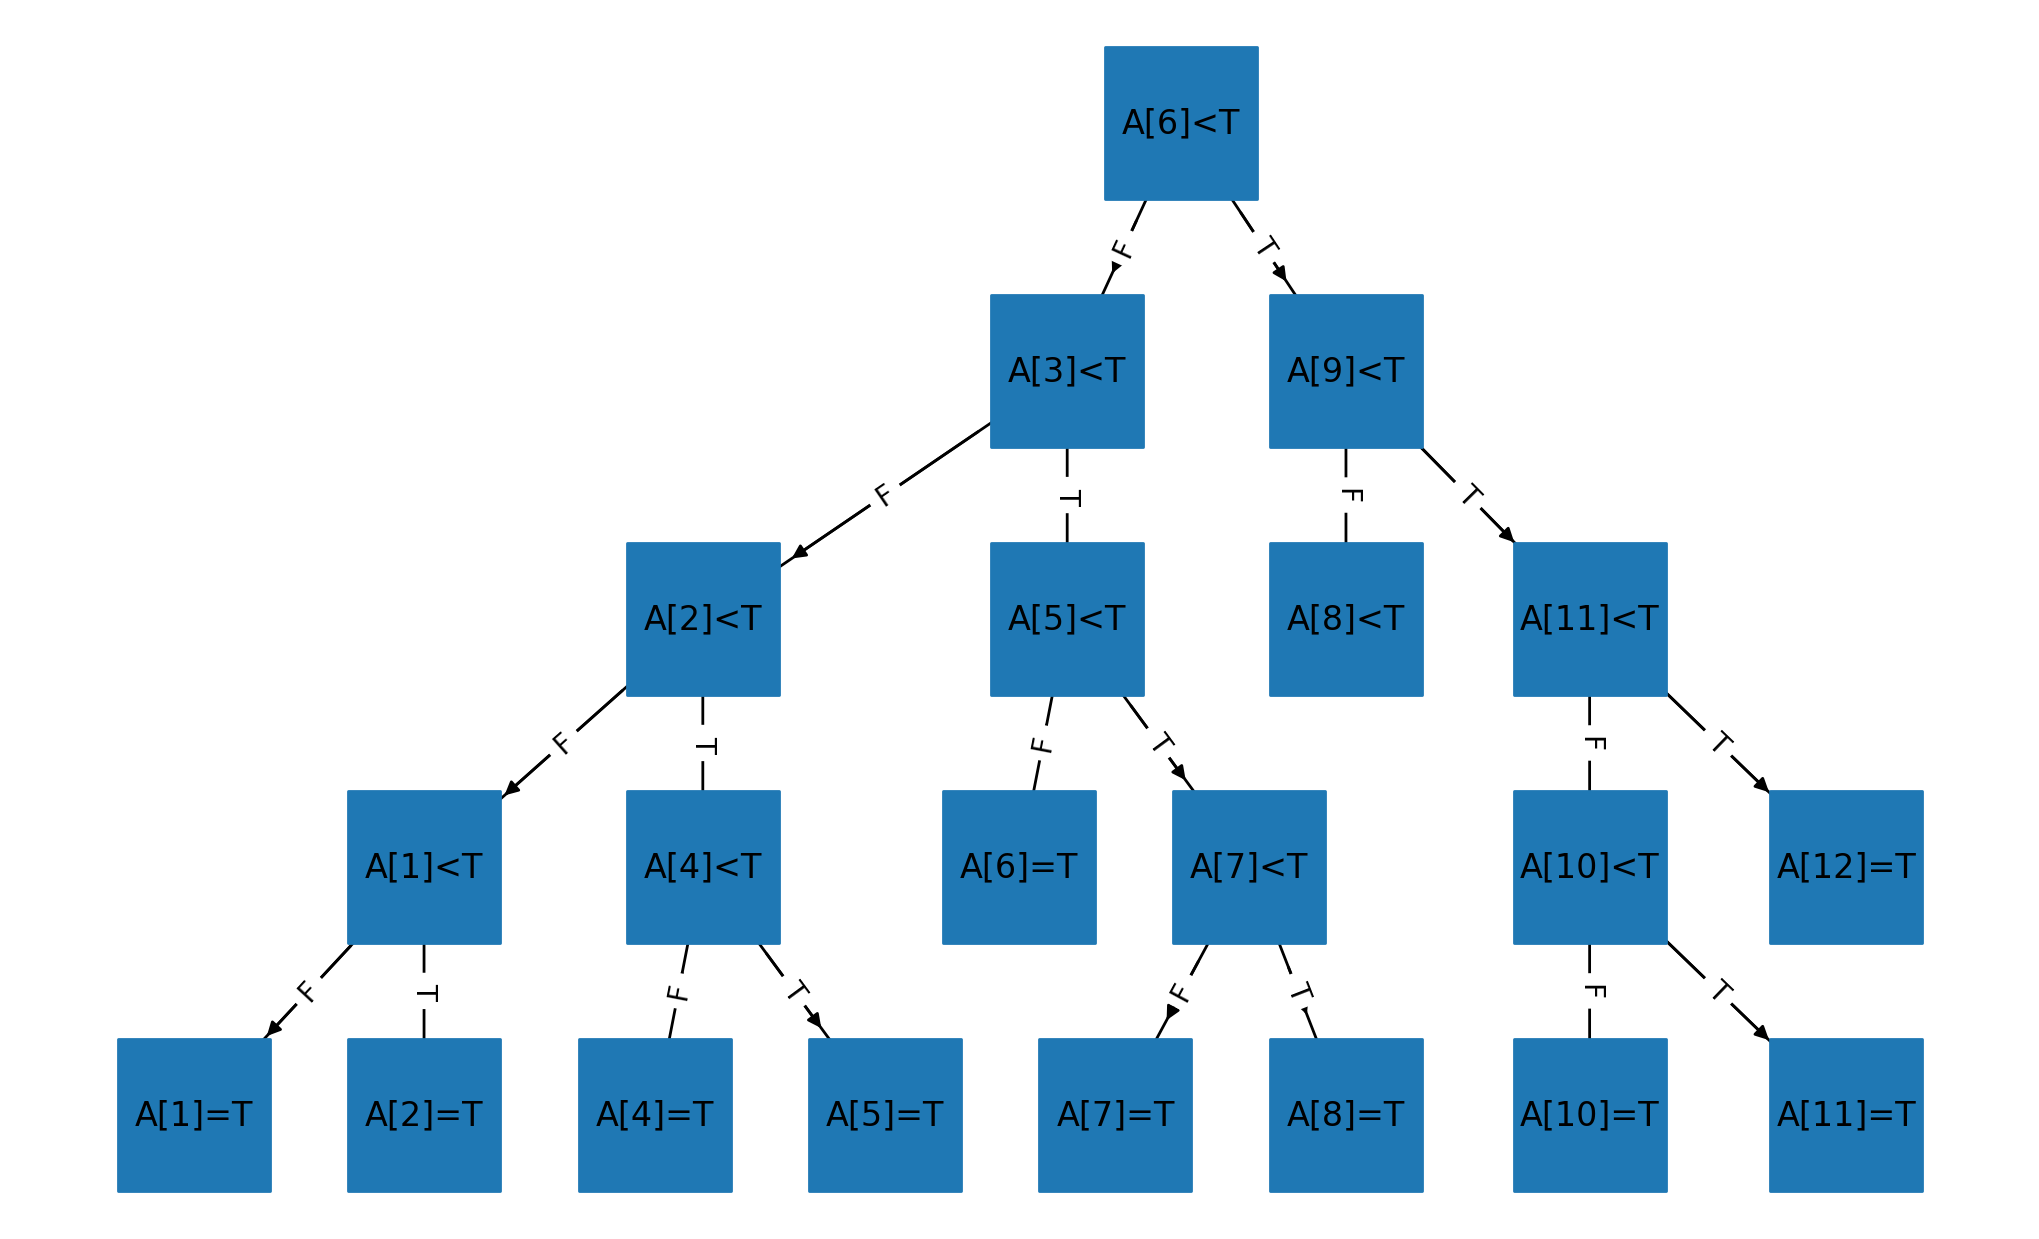
\includegraphics[width = 1\textwidth]{v2bintree.png}
        \caption{Binary Search V2 with $n=12$}
    \end{figure}
    This diagram is also a Binary Tree. But in it, from every internal vertex, there
    are exactly two edges downward in the diagram (never just one). This kind of
    Binary Tree is said to be a full Binary Tree. We will look into trees in detail in the next section.
    \begin{theorem}
        If \( T \) is a full binary tree with \( m \) internal vertices, then \( T \) has \( m + 1 \) leaves.
        \end{theorem}
        
        \begin{proof}
        We proceed by induction on the number of internal vertices, \( m \).
        
        \textbf{Base Case:} When \( m = 1 \), there is only one internal vertex, which is the root of the tree. By the definition of a full binary tree, the root must have two children, and since these children cannot be internal vertices (as there is only one internal vertex, the root itself), they must be leaves. Hence, the tree has \( 1 + 1 = 2 \) leaves, which satisfies our theorem.
        
        \textbf{Inductive Step:} Assume that the theorem holds for a full binary tree with \( m \) internal vertices, such that the tree has \( m + 1 \) leaves. Now consider a full binary tree with \( m + 1 \) internal vertices. By the definition of a full binary tree, adding an internal vertex means we are adding two children to an existing leaf (which is now converted into an internal vertex). This addition results in one less leaf (the converted internal vertex) and two more leaves (the new children). Therefore, the number of leaves increases by \( 2 - 1 = 1 \) compared to the number of leaves in the tree with \( m \) internal vertices.
        
        So, a tree with \( m + 1 \) internal vertices will have \( (m + 1) + 1 \) leaves. Hence, by the principle of mathematical induction, the theorem is true for all \( m \geq 1 \).
        \end{proof}
    \subsection{Exercises}
    \begin{exercise}
        Suppose \( T \) is not found by Binary Search. Where will \( T \) fit into the array? 
        Where should it be inserted?
    \begin{enumerate}
        \item Is the final \( q \)-value always one less than the final \( p \)-value?
        \item When is \( A[q] < T < A[p] \)?
        \item If \( p = 1 \) (that is, \( p \) was never changed), is \( T < A[1] \)?
        \item If \( q = n \) (that is, \( q \) was never changed), is \( A[n] < T \)?
    \end{enumerate}
    \end{exercise}
    
    \textbf{Solution}:
    \begin{enumerate}
        \item The final value of \( q \) is not necessarily always one less than the final \( p \) value. It depends on the search process and the position where \( T \) would fit if it were in the array.
        \item The condition \( A[q] < T < A[p] \) holds when \( T \) would be inserted between \( A[q] \) and \( A[p] \) in a sorted array to maintain the sorted order.
        \item If \( p = 1 \), it means \( T < A[1] \), and \( T \) should be inserted at the beginning of the array.
        \item If \( q = n \), it means \( A[n] < T \), and \( T \) should be inserted at the end of the array.
    \end{enumerate}


    \begin{exercise}
        Consider the best performance of binary search in $\Theta$ notation and worst performance in big $O$ notation. Is it possible to get the average performance in $\Theta$ notation? If yes, state the precise time complexity; if not, explain why.
    \end{exercise}
    \textbf{Solution:}

    \begin{itemize}
        \item Best time complexity: The best case scenario occurs when the target value is at the midpoint of the array, which happens with a constant time complexity, thus $\Omega(1)$. However, best case scenarios are generally not described using $\Theta$ notation as it implies a tight bound that is both the upper and lower limit, which is not applicable for the best case.
        \item Worst time complexity: Binary search has a worst-case time complexity of $O(\log n)$ when the target value is not within the initial bounds of the midpoint checks, thus requiring the maximum number of iterations to converge on the target.
        \item Average time complexity: The average time complexity of binary search is generally represented as $O(\log n)$. This is due to the fact that, on average, the number of steps required to find an element in a sorted array is logarithmic relative to the array size. Precise average case analysis of binary search is complex as it depends on the probability distribution of the target element's position. It is generally not represented in $\Theta$ notation because the lower and upper bounds for the average case cannot be tightly bounded as they can be for the best and worst cases.
    \end{itemize}
    
    \begin{exercise}
        Prove by MI that $\displaystyle \forall \ k\in \mathbb{N} ,\ $if Binary Search is applied to an array of length$\displaystyle \ n$ and has not terminated after $\displaystyle k$ (unsuccessful) probes, then the length of the current sublist must be less or equal to $\displaystyle \frac{n}{2^{k}}$
    \end{exercise}
    \begin{proof}
        We use $\displaystyle L(w)$ to denote the length of the current sublist after $\displaystyle w$ probes.
        
        \textbf{Base Case:}
        When $\displaystyle k=0$, the sorting is not yet started, so $\displaystyle L( 0) =n$, and we have $\displaystyle L( 0) =\frac{n}{2^{0}} =n$.
        
        \textbf{Inductive hypothesis:}
        Now assume that when $\displaystyle k=w$, it holds that:
        \begin{equation*}
        L( w) \leq \frac{n}{2^{w}}
        \end{equation*}
        
        \textbf{Inductive Step:}
        Thus, we need to prove that for $\displaystyle k=w+1$, $\displaystyle L( w+1) \leq 
        \frac{n}{2^{w+1}}$.
        We have proven earlier in theorem \ref{4.2.1} that after $\displaystyle w$ loops, $\displaystyle 
        \lfloor n/2^{w} \rfloor \leq L( w) \leq \lceil n/2^{w} \rceil $, and the length of the 
        sublist to be probed after $\displaystyle k+1$ unsuccessful probes is $\displaystyle 
        \frac{n}{2^{w+1}}$. While \ $\displaystyle \frac{n}{2^{w+1}} \leq \lceil n/2^{w+1} \rceil $. 
        Refer to the definition of $\displaystyle w( k)$ in the statement of problem, $\displaystyle 
        w\in \mathbb{N}$, so $\displaystyle \frac{n}{2^{w+1}} =\lceil n/2^{w+1} \rceil \ $. Hence, $\displaystyle L( w+1) \ \leq \frac{n}{2^{w+1}} \ $, this completes the proof.
    \end{proof}
    
\end{comment}


\chapterimage{orange2.jpg}
\chapterspaceabove{6.75cm} 
\chapterspacebelow{7.25cm} 
\chapter{Graph Theory}
\begin{remark}
    This chapter involves the knowledge of combinatorics, which is in chapter \ref{counting}.
    You may read through that chapter from basic counting method to random variables.
    If you have learned what have been discussed so far, those content will not cause
    too many troubles. Do at least read through \textbf{Permutation and Combination}
    before dive into this chapter.
\end{remark}

\chapterimage{orange2.jpg}
\chapterspaceabove{6.75cm} 
\chapterspacebelow{7.25cm} 
\chapter{Basics of Abstract Algebra}
\lipsum
\section{Fundamentals of Algebraic Structures}
    \subsection{Groups}
    \subsection{Rings}
    \subsection{Fields}
    \subsection{Exercises}
\section{Operations on Algebraic Structures}
    \subsection{Homomorphisms}
    \subsection{Isomorphisms}
    \subsection{Exercises}
\section{Applications of Algebraic Structures}
    \subsection{Cryptography}
    \subsection{Coding Theory}
    \subsection{Exercises}

\chapterimage{orange2.jpg}
\chapterspaceabove{6.75cm} 
\chapterspacebelow{7.25cm} 
\chapter{Introductory Topology and Category Theory}
\lipsum


\section{Basic Topology}
\lipsum
\subsection{Introduction to Topological Spaces}
\subsubsection{Open and Closed Sets}
\subsubsection{Basis for a Topology}
\subsection{Continuity and Limits}
\subsubsection{Continuous Functions}
\subsubsection{Limit Points and Convergence}
\subsection{Compactness and Connectedness}
\subsubsection{Compact Spaces}
\subsubsection{Connected Spaces}
\subsection{Applications of Topology}
\subsubsection{Topology in Computer Science}
\subsubsection{Topology in Physics}

\section{Category Theory Fundamentals}
\lipsum
\subsection{Introduction to Categories}
\subsubsection{Objects and Morphisms}
\subsubsection{Examples of Categories}
\subsection{Functors and Natural Transformations}
\subsubsection{Definition of Functors}
\subsubsection{Natural Transformations between Functors}
\subsection{Limits and Colimits}
\subsubsection{Universal Properties}
\subsubsection{Construction of Limits and Colimits}
\subsection{Applications of Category Theory}
\subsubsection{Category Theory in Programming Languages}
\subsubsection{Category Theory in Logic and Set Theory}
%------------------------------------------------
\part{Single-variable Calculus}
\chapterimage{orange2.jpg}
\chapterspaceabove{6.75cm} 
\chapterspacebelow{7.25cm} 
\chapter{Function Monotonicity, Parity and Periodicity}

    \section{Monotonicity of Function}


    \section{Parity of Function}


    \section{Periodicity of Function}
\chapterimage{orange2.jpg}
\chapterspaceabove{6.75cm} 
\chapterspacebelow{7.25cm} 
\chapter{Abstract and Piece-wise Function}

    \section{Abstract Function}

    \section{Piece-wise Function}
\chapterimage{orange2.jpg}
\chapterspaceabove{6.75cm} 
\chapterspacebelow{7.25cm} 
\chapter{Limit and Continuity}
    \section{Limit of Sequence}


    \section{limit of Function}


    \section{Continuity}


    \section{Application of Limit}
\chapterimage{orange2.jpg}
\chapterspaceabove{6.75cm} 
\chapterspacebelow{7.25cm} 
\chapter{Differential Calculus}

    \section{Derivative Basics}
        \subsection{Definition of Derivative}
        \subsection{Geometric Meaning of Derivative}
        \subsection{Physical Meaning of Derivative}

    \section{Basic Derivative Rules}
        \subsection{Derivatives of Elementary Functions}
        \subsection{Product Rule, Quotient Rule, Chain Rule}

    \section{Higher-order Derivatives}
        \subsection{Second-order Derivatives and Applications}
        \subsection{Calculation and Significance of Higher-order Derivatives}

    \section{Derivatives of Abnormal Function}
        \subsection{Derivatives of Implicit Functions}
        \subsection{Derivatives of Parametric Equations}

    \section{Differentiation}
    
    \section{Related Rates}
        \subsection{Relationships between Rates of Change of Different Quantities}

    \section{Taylor Series}
        \subsection{Taylor Expansion of Functions}
        \subsection{Application of Taylor Series}
    

    \section{Applications of Differential Calculus}
        \subsection{Tangents and Normals of Curves}
        % \subsection{Analysis of Velocity and Acceleration in Motion}
        \subsection{Mean Value Theorem in Differential Calculus}
        \subsubsection{Fermat's Theorem}
        \subsubsection{Rolle's Theorem}
        \subsubsection{Lagrange's Mean Value Theorem}
        \subsubsection{Cauchy's Mean Value Theorem}
        \subsubsection{Indeterminate Form Limit}
        \subsection{Extrema Problems and Optimization}
\chapterimage{orange2.jpg}
\chapterspaceabove{6.75cm} 
\chapterspacebelow{7.25cm} 
\chapter{integral calculus}

\section{Fundamentals of Integration}
    \subsection{Definition of the Integral}
    \subsection{Properties of Integrals}
    \subsection{The Fundamental Theorem of Calculus}

\section{Techniques of Integration}
    \subsection{Basic Integration Formulas}
    \subsection{Integration by Substitution}
    \subsection{Integration by Parts}
    \subsection{Trigonometric Integrals}
    \subsection{Partial Fractions}

\section{Applications of Integration}
    \subsection{Area Under Curves}
    \subsection{Volumes of Solids of Revolution}
    \subsection{Arc Length and Surface Area}
    \subsection{Center of Mass and Moments}

\section{Improper Integrals}
    \subsection{Convergence and Divergence of Improper Integrals}
    \subsection{Applications of Improper Integrals}

\section{Numerical Integration Methods}
    \subsection{The Trapezoidal Rule}
    \subsection{Simpson's Rule}
\chapterimage{orange2.jpg}
\chapterspaceabove{6.75cm} 
\chapterspacebelow{7.25cm} 
\chapter{Differential Equation}
\chapterimage{orange2.jpg}
\chapterspaceabove{6.75cm} 
\chapterspacebelow{7.25cm} 
\chapter{Infinite Series}
%------------------------------------------------
\part{Multi-variable and Vector Calculus}
\chapterimage{orange2.jpg}
\chapterspaceabove{6.75cm} 
\chapterspacebelow{7.25cm} 
\chapter{integral calculus}


\chapterimage{orange2.jpg}
\chapterspaceabove{6.75cm} 
\chapterspacebelow{7.25cm} 
\chapter{Introduction to Multivariable Functions}
    \subsection{Concepts of Multivariable Functions}
    \subsection{Graphs and Contour Plots}


\chapterimage{orange2.jpg}
\chapterspaceabove{6.75cm} 
\chapterspacebelow{7.25cm} 
\chapter{Partial Derivatives}
    \subsection{Definition and Interpretation}
    \subsection{Higher-Order Partial Derivatives}
    \subsection{Chain Rule in Multiple Variables}


\chapterimage{orange2.jpg}
\chapterspaceabove{6.75cm} 
\chapterspacebelow{7.25cm}     
\chapter{Multiple Integrals}
    \subsection{Double Integrals}
    \subsubsection{Iterated Integrals}
    \subsubsection{Double Integrals over General Regions}
    \subsection{Triple Integrals}
    \subsubsection{Cylindrical and Spherical Coordinates}


\chapterimage{orange2.jpg}
\chapterspaceabove{6.75cm} 
\chapterspacebelow{7.25cm}     
\chapter{Vector Calculus}
    \section{Vector Fields}
    \section{Gradient, Divergence, and Curl}
    \section{Line and Surface Integrals}
%------------------------------------------------
\part{Linear Algebra}
\chapterimage{orange2.jpg}
\chapterspaceabove{6.75cm} 
\chapterspacebelow{7.25cm} 
\chapter{Vectors Space and the Geometry of Space}






\chapterimage{orange2.jpg}
\chapterspaceabove{6.75cm} 
\chapterspacebelow{7.25cm} 
\chapter{Matrices and Systems of Equations}


\chapterimage{orange2.jpg}
\chapterspaceabove{6.75cm} 
\chapterspacebelow{7.25cm} 
\chapter{Determinant of Matrix}


\chapterimage{orange2.jpg}
\chapterspaceabove{6.75cm} 
\chapterspacebelow{7.25cm} 
\chapter{Orthogonality}


\chapterimage{orange2.jpg}
\chapterspaceabove{6.75cm} 
\chapterspacebelow{7.25cm} 
\chapter{Linear Transformations}

\chapterimage{orange2.jpg}
\chapterspaceabove{6.75cm} 
\chapterspacebelow{7.25cm} 
\chapter{Eigenvalues and Eigenvector}


\chapterimage{orange2.jpg}
\chapterspaceabove{6.75cm} 
\chapterspacebelow{7.25cm} 
\chapter{Singular Value Decomposition}


\chapterimage{orange2.jpg}
\chapterspaceabove{6.75cm} 
\chapterspacebelow{7.25cm} 
\chapter{Complex Vector and Matrices}



\chapterimage{orange2.jpg}
\chapterspaceabove{6.75cm} 
\chapterspacebelow{7.25cm} 
\chapter{Matrix Differential Calculus}
%------------------------------------------------
\part{Probability and Combinatorics}
\chapterimage{orange2.jpg}
\chapterspaceabove{6.75cm} 
\chapterspacebelow{7.25cm} 



\chapter{Introduction to Counting and Probability }\label{counting}
In this part, we discuss wider topics on probability and probability distributions. 
Probability theory is a branch of mathematics that deals with the analysis of random phenomena. The fundamental concept of the theory is the probability measure, a way of assigning a number to each plausible outcome of an event in such a way that the number reflects the event's likelihood of occurring. This mathematical framework allows for the study and modeling of uncertainty and complexity in various fields, ranging from physics and biology to economics and psychology. By providing the tools to make quantitative predictions about the likelihood of certain outcomes, probability theory forms the basis for statistical inference, enabling scientists and statisticians to infer properties about a population given a sample. The origins of probability theory can be traced back to the analysis of games of chance and has since evolved into a vital component of both theoretical and applied mathematics.

    \section{Counting Principal}
    The very first section in this chapter focuses on the basics of counting, which is the foundation of the whole probability theory. In the study of probability, we aim to measure 
    random events, and to do this, we must know their frequency, or rather, how many possible outcomes each event has. Counting method allows us to get the possible number of outcomes in a 
    systematic way.

    \subsection{Principal of Counting}
    We may start with the most basic counting. Considering tossing a coin, and we make the assumption that this coin is unbiased, meaning that the chance of getting a chance or tail must be 
    exactly $\frac{1}{2}$. In this case, the total possible number of outcome is 2. This conclusion is obviously true and can be obtained by intuition, because we cannot find a third case that the result is neither a head nor a tail, as the event
    is binary.

    Now let's increase the number of trials, how many outcomes can we have when tossing a coin twice? If we use T to denote that the result is a head and F for the tail, like what we have
    done in Boolean Algebra, we have 4 ways to arrange the possibilities:
    $$(T,T), (T,F), (F,T),(F,F).$$
    Thus we conclude that we have 4 possible outcomes. 

    This example lead us to a fundamental theorem in counting.
    \begin{theorem}[The Basic Principal of Counting]\label{Principal of Counting}
        Suppose that two experiments are to be performed. Then if experiment1 can
        result in any one of $m$ possible outcomes and if, for each outcome of experiment 1, there are $n$ possible outcomes of experiment 2, then together there are $mn$
        possible outcomes of the two experiments.
    \end{theorem}

    This theorem could be proved by mathematical induction.
    \begin{proof}
        Start with the base case of $m = n = 1$, there are only 1 possible combination of event 1 and event 2.
        We move on to the case when $m = n = 2$, there are $4 = 2\times 2$ outcomes: $(1, 1), (1, 2), (2, 1), (2, 2)$.
        Suppose that the number of outcomes for each event are any integer $n \in \mathbb{N}^+$, similarly, we can enumerate all the cases from $(1, 1)$ to $(n, n)$,  $n^2 = n\times n$ outcomes.
        For the case when the number of outcomes coming to $n+1$. We can still enumerate all $(n+1)^2 = (n+1)\times(n+1)$ outcomes in a similar way.
        \par Therefore, the theorem is proven. This could be visualized by $$\begin{array}{l}(1,1),(1,2), \ldots,(1, n) \\(2,1),(2,2), \ldots,(2, n) \\\vdots \\(m, 1),(m, 2), \ldots,(m, n)\end{array}$$
    \end{proof}

    \begin{example}
        A small community consists of 10 women, each of whom has 3 children. If one woman and one of her children are to be chosen as mother and child of the year,
        how many choices are possible?
    \end{example}
        \begin{solution}
            By theorem\ref{Principal of Counting}, the event chosen as woman has $m=10$ outcomes, while there are $n = 3$ outcomes for choosing children. 
            Hence the total combinations will be $m\times n = 10\times 3 =30 $
        \end{solution}
    But mathematicians hate listing possible cases. Is there a way to describe the relation between the trial of events and number
    of possible outcomes? Think about the way we treat Boolean variables in the truth table, to get the possible outcomes, we arrange them in all possible ways to get a complete
    truth table. Just like what we do here, we are making trials twice here for tossing coins, each trial has 2 outcomes, and when we make a truth table, we are generating combinations of
    Boolean value, and we know that $n$ Boolean variable has $2^n$ ways of arrangement. So we can say that tossing a coin here could be fitted into this relation when $n=2$, and they are
    actually equivalent in terms of  counting the number of outcomes. With this, we can deduce that if we toss the coin for $n$ times, we also have $2^n$ outcomes.

    This allows us to generalize theorem \ref{Principal of Counting}.

    \begin{theorem}[The Generalized Principal of Counting]\label{Generalized Principal of Counting}
        If $r$ experiments that are to be performed are such that the first one may result in any of $n_1$ possible outcomes; and if, for each of these $n_1$  possible outcomes,
        there are $n_2$  possible outcomes of the second experiment; and if, for each of the possible outcomes of the first two experiments, there are $n_3$  possible outcomes
        of the third experiment; and if ..., then there is a total of  $\Pi_{k=1}^r{n_k} = n_1 \cdot n_2 \dots n_r$ possible outcomes of the $r$ experiments.
    \end{theorem}

    Similarly, this theorem could be proven by mathematical induction with theorem\ref{Principal of Counting} as a lemma. We leave this proof as an exercise.

    This theorem also what we call product rule of counting, which also applicable to probability, which we will discuss in the next section.

    Now we introduce another parallel theorem known as addition rule of counting. This is even easier to understand, suppose 
    \begin{theorem}[Addition Rule of Counting]\label{Adittion Rule}
        Suppose that an experiment can be performed in one of $m$ ways \textbf{or} in one of $n$ ways. Where none of the $n$ ways are the same as the $m$
        ways, then there are $m+n$ ways to perform it.
    \end{theorem}
    This theorem could be proven directly by using set.
    \begin{proof}
        Let \( A \) and \( B \) be finite sets such that \( A \cap B = \emptyset \). By the definition of disjoint sets, no element is in both \( A \) and \( B \).
        
        Let \( a_i \) be an element in \( A \) and \( b_j \) be an element in \( B \), for \( i = 1, 2, \ldots, n \) and \( j = 1, 2, \ldots, m \). The set \( A \) contains exactly \( n \) elements and \( B \) contains exactly \( m \) elements.
        
        The union \( A \cup B \) is a set containing all the elements \( a_i \) and \( b_j \) without any repetition, since \( A \) and \( B \) are disjoint.
        
        Therefore, the set \( A \cup B \) has \( n + m \) elements, which proves the theorem.
        \end{proof}
    \begin{example}
        A student can choose a computer project from one of three lists. The three lists contain 23, 15, and 19 possible projects, respectively. 
        No project is on more than one list. How many possible projects are there to choose from?
    \end{example}
    \begin{solution}
        By addition rule, the student can choose a project by selecting a project from the first list, the second list, or the third list. Because no project is on more than one list, 
        by the sum rule there are $23 + 15 + 19 = 57$ ways to choose a project.
    \end{solution}

    \begin{example}
        How many different license plates can be made if each plate contains a sequence of three uppercase English letters followed by three digits (and no sequences of letters are prohibited, even if they are obscene)?
    \end{example}
        
        \begin{solution}
        To determine the number of different license plates possible, we use the rule of product, also known as the counting principle. 
        
        Each of the three positions for the letters can be filled with any of the 26 letters of the English alphabet. Similarly, each of the three positions for the digits can be filled with any of the 10 digits from 0 to 9.
        
        Therefore, the total number of possible license plates is given by:
        \[ 26 \times 26 \times 26 \times 10 \times 10 \times 10 = 26^3 \times 10^3 \]
        
        Calculating the powers, we get:
        \[ 26^3 = 26 \times 26 \times 26 = 17576 \]
        \[ 10^3 = 10 \times 10 \times 10 = 1000 \]
        
        Multiplying these together, we find the total number of different license plates that can be made:
        \[ 17576 \times 1000 = 17576000 \]
        
        Hence, there are 17,576,000 different possible license plates.
        \end{solution}
        
        To correctly count the number of ways to do the two tasks, we must subtract the number of ways that are counted twice. This leads us to an important counting rule.
        Actually, we have already covered this conclusion in set theory.

        The Subtraction Rule in set theory is a straightforward concept used when we need to find the number of elements in a set by excluding those that meet certain criteria. It states that if we have a universal set \( U \) and a subset \( A \) that we wish to exclude, then the number of elements not in \( A \) is \( |U| - |A| \), where \( |S| \) denotes the cardinality of set \( S \).

        The Principle of Inclusion-Exclusion extends the Subtraction Rule for multiple sets. It corrects the overcounting that occurs when we subtract the cardinalities of overlapping sets from the universal set. For two sets \( A \) and \( B \), it is given by \( |A \cup B| = |A| + |B| - |A \cap B| \).
        
        \begin{theorem}[Subtraction Rule]
            If a task can be done in either $n_1$ ways or $n_2$ ways, then the number of ways to do the task is $n_1+n_2$ minus the number of ways to do the task that are common to the two different ways.
        \end{theorem}
        Here are two examples demonstrating these rules.
        \begin{example}
            Suppose a library has 1,000 books, 300 of which are fiction. If we want to know how many books are non-fiction, we can use the Subtraction Rule:
            $$ \text{Number of non-fiction books} = |U| - |A| = 1,000 - 300 = 700. $$
        \end{example}

        \begin{example}
            In a survey of 200 people, 120 say they like tea, and 150 like coffee. If 50 people like both tea and coffee, to find out how many people like either tea or coffee, we apply the Principle of Inclusion-Exclusion:
            $$ \text{Number of people who like tea or coffee} = |A| + |B| - |A \cap B| = 120 + 150 - 50 = 220. $$
        \end{example}

        We also have division rule of counting, which could be further explained by equivalence class. 
        \begin{theorem}[Rule of Division]
            The rule of division states that there are $n/d$ ways to do a task if it can be done using a procedure that can be carried out in 
                $n$ ways, and for each way $w$, exactly $d$ of the $n$ ways correspond to the way $w$. In a nutshell, the division rule is a common way to ignore "unimportant" differences when counting things.
        \end{theorem}
            This theorem could be further explained by congruence class.
            \begin{example}
                Suppose a set \(X\) with \(n\) elements is partitioned into \(k\) equivalence classes by an equivalence relation, and each equivalence class contains \(m\) elements. If we wish to count the number of distinct subsets of \(X\) that can be formed without regard to the ordering of elements within each equivalence class, we can apply the Division Rule. Since each equivalence class is indistinguishable in terms of the partition, the total number of distinct subsets is \(n/m\), where \(n\) is the total number of elements in the set, and \(m\) is the number of elements in each equivalence class.
            \end{example}

            \begin{example}
                If the total degree of a graph is 58, how many edges does it have?
            \end{example}
            \begin{solution}
                hen we count the degrees, we count each edge twice, so there are 58/2 = 29 edges.
            \end{solution}
    \subsection{Pigeonhole Theorem}
        We also have another useful conclusion on counting called pigeonhole theorem. Suppose we have 8 pigeons and 7 pigeonholes, then there must be one pigeonhole that
        holds 2 pigeons.
        \begin{theorem}[pigeonhole theorem]
            If $k$ is a positive integer and $k+1$ or more objects are placed into $k$ boxes, then there is at least one box containing two or more of the objects.
        \end{theorem}
        
        \begin{proof}
            We prove the pigeonhole principle using a proof by contraposition. Suppose that none of the $k$ boxes contains more than one object. Then the total number of objects would be 
            at most $k$ This is a contradiction, because there are at least $k+1$ objects.
        \end{proof}
        This theorem could also be generalized.
        \begin{theorem}[Generalized Pigeonhole Principle]
            If \( N \) objects are placed into \( k \) boxes, then there is at least one box containing at least \( \lceil N/k \rceil \) objects.
            \end{theorem}
            
            \begin{proof}
            We will prove the statement by contraposition. Let us assume that no box contains \( \lceil N/k \rceil \) or more objects. This means each box has at most \( \lceil N/k \rceil - 1 \) objects.
            And the number of objects being placed cannot be $N$, so we have the number of object less than $N$ (this is obvious because it can't be greater than $N$). 
            
            The total number of objects, under this assumption, can be represented by multiplying the number of boxes by the maximum number of objects each box could contain:
            \[
            k \left( \left\lceil \frac{N}{k} \right\rceil - 1 \right)
            \]
            Using the property that \( \lceil x \rceil \leq x + 1 \) for any real number \( x \), we substitute \( \frac{N}{k} \) for \( x \) to obtain:
            \begin{remark}
                We get this result in integer function, just in case that you don't remember...
            \end{remark}
            \[
            \left\lceil \frac{N}{k} \right\rceil \leq \frac{N}{k} + 1
            \]
            Applying this to our previous equation:
            \[
            k \left( \left\lceil \frac{N}{k} \right\rceil - 1 \right) < k \left( \frac{N}{k} + 1 - 1 \right) = N
            \]
            This shows that the total number of objects is less than \( N \) under our initial assumption, which is a contradiction since we started with \( N \) objects.
            
            Thus, the contrapositive has been proven true: if all boxes have fewer than \( \lceil N/k \rceil \) objects, then we do not have \( N \) objects. Therefore, by contraposition, the original statement is also true: if \( N \) objects are placed into \( k \) boxes, there must be at least one box with \( \lceil N/k \rceil \) or more objects.
            \end{proof}
            
        \begin{example}
            \begin{itemize}
                \item Among any group of 367 people, there must be at least two with the same birthday, because
                there are only 366 possible birthdays.
                \item In any group of 27 English words, there must be at least two that begin with the same letter,
                because there are 26 letters in the English alphabet.
            \end{itemize}
        \end{example}

        \begin{example}
            What is the minimum number of students required in a discrete mathematics class to be sure that at least six will receive the same grade, if there are five possible grades, A, B, C, D, and F?
            \end{example}
            
            \begin{proof}
            The minimum number of students needed to ensure that at least six students receive the same grade can be found using the Pigeonhole Principle. According to this principle, if \(N\) objects (in this case, students) are distributed among \(k\) categories (in this case, grades), and if \(N > k \cdot (m-1)\) where \(m\) is the minimum number of objects that we want in at least one category, then at least one category must contain at least \(m\) objects.
            
            Here, we want \(m = 6\) students to have the same grade and we have \(k = 5\) grades. We can apply the formula to find the minimum \(N\):
            
            \[ N > 5 \cdot (6-1) \]
            \[ N > 25 \]
            
            The smallest integer greater than 25 is 26, so at least 26 students are needed to guarantee that at least six will receive the same grade. If we had only 25 students, it could happen that each of the five grades is assigned to exactly five students, which means no grade would have six students. Therefore, 26 is the minimum number of students required to ensure that at least six students will receive the same grade.
            \end{proof}


    \subsection{Exercises}
    \begin{exercise}
        Prove the Generalized Principal of Counting.
    \end{exercise}
    \begin{proof}
        We proceed by mathematical induction on \( r \), the number of experiments.
        
        \textbf{Base Case:} For \( r = 1 \), the theorem trivially holds since there are \( n_1 \) possible outcomes for the single experiment.
        
        \textbf{Inductive Step:} Assume that the theorem holds for \( r = k \), that is, there are \( \prod_{i=1}^k n_i \) outcomes for \( k \) experiments. Now consider \( r = k + 1 \) experiments. For the first \( k \) experiments, by the inductive hypothesis, we have \( \prod_{i=1}^k n_i \) outcomes. For each of these outcomes, the \( (k+1)^{th} \) experiment can have \( n_{k+1} \) outcomes. Therefore, the total number of outcomes for \( k + 1 \) experiments is:
        
        \[
        \left( \prod_{i=1}^k n_i \right) \cdot n_{k+1} = \prod_{i=1}^{k+1} n_i
        \]
        
        This completes the inductive step and thus the proof.
    \end{proof}
        
    \begin{exercise}
        How many functions are there from a set with $m$ elements to a set with $n$ elements?
    \end{exercise}
    \begin{solution}
        A function corresponds to a choice of one of the $n$ elements in the codomain for each of
        the $m$ elements in the domain. Hence, by the product rule there are $n\cdot n\cdot\cdots\cdot n=n^m$ functions from a set with $m$ elements to one with $n$ elements. 
    \end{solution}

    \begin{exercise}
        How many one-to-one functions are there from a set with $m$ elements to one with $n$ elements?
    \end{exercise}
        \begin{solution}
            First note that when $m>n$ there are no one-to-one functions from a set with $m$ elements to a set with $n$ elements.
            
            Now let $m\leq n.$ Suppose the elements in the domain are $\alpha_1,\alpha_2,\ldots,\alpha_m$ .There are $n$ ways to choose the value of the function at $\alpha_1.$ 
            Because the function is one-to-one, the value of the function at $\alpha_{2}$ can be picked in $n-1$ ways (because the value used for $\alpha_{1}$ cannot be used again). 
            In general, the value of the function at $a_k$ can be chosen in $n-k+1$ ways. By the product rule, there are $n(n-1)(n-2)\cdots(n-m+1)$ one-to-one functions from a set 
            with $m$ elements to one with $n$ elements.
        \end{solution}

    \begin{exercise}
        Prove that if \( A_1, A_2, \ldots, A_m \) are finite sets, then the number of elements in the Cartesian product of these sets is the product of the number of elements in each set.
    \end{exercise}
        
        \begin{proof}
        Consider the finite sets \( A_1, A_2, \ldots, A_m \) with respective cardinalities \( |A_1|, |A_2|, \ldots, |A_m| \). The Cartesian product \( A_1 \times A_2 \times \cdots \times A_m \) is defined as the set of all ordered \( m \)-tuples \( (a_1, a_2, \ldots, a_m) \) where \( a_i \in A_i \) for each \( i \).
        
        To construct an element of the Cartesian product, we must choose an element from each set \( A_i \). The number of ways to choose an element from \( A_1 \) is \( |A_1| \), from \( A_2 \) is \( |A_2| \), and so on, until \( A_m \) which is \( |A_m| \).
        
        By the product rule of counting, the total number of ways to make these choices is the product of the number of choices for each set, which gives us:
        
        \[ |A_1 \times A_2 \times \cdots \times A_m| = |A_1| \cdot |A_2| \cdot \ldots \cdot |A_m| \]
        
        This product counts the number of distinct ordered \( m \)-tuples that can be formed, which is exactly the number of elements in the Cartesian product \( A_1 \times A_2 \times \cdots \times A_m \). Hence, the proof is complete.
        \end{proof}
    
    \begin{exercise}
        Let $A$ and $B$ be finite sets. $|A| = k+1$, $|B| = k$, prove that there is no one-to-one function defined in the mapping $A \to B$.
    \end{exercise}
        \begin{solution}
            By pigeonhole theorem, we have $k+1$ pigeons but only $k$ pigeonholes, so one pigeonhole must have $\lceil k+1/k \rceil = 2$ pigeonholes. This means that there is always one
            element from the codomain are mapped from the same element in the domain. Hence, the statement is proven.
        \end{solution}
        \begin{exercise}
            How many cards must be selected from a standard deck of 52 cards to guarantee that:
            \begin{enumerate}
                \item[a)] At least three cards of the same suit are selected?
                \item[b)] At least three hearts are selected?
            \end{enumerate}
            \end{exercise}
            
            \begin{solution}
            \textbf{a)} Suppose there are four boxes, one for each suit, and as cards are selected they are placed in the box reserved for cards of that suit. By the generalized pigeonhole principle, we see that if \( N \) cards are selected, there is at least one box containing at least \( \lceil N/4 \rceil \) cards. To ensure that at least three cards of one suit are selected, we need \( \lceil N/4 \rceil \geq 3 \). The smallest integer \( N \) satisfying this condition is \( N = 2 \cdot 4 + 1 = 9 \), since selecting 8 cards could result in two cards of each suit, but the ninth card guarantees three of one suit.
            
            \textbf{b)} Without the pigeonhole principle, we consider the worst-case scenario where the selected cards are all from the clubs, diamonds, and spades suits. There are 13 cards in each suit, so after selecting all 39 of these, the next three cards must be hearts. Therefore, we may need to select up to 42 cards to guarantee three hearts.
        \end{solution}
            

    \begin{exercise}
        Let \( X = \{a, b, c, d\} \).
        \begin{enumerate}
            \item[(a)] How many possible relations are there on \( X \)?
            \item[(b)] How many of these are reflexive?
            \item[(c)] How many of these are reflexive and symmetric?
            \item[(d)] How many of these are equivalence relations?
            \item[(e)] What would the answers to (a), (b) and (c) be if \( |X| = n \) instead of \( |X| = 4 \)?
        \end{enumerate}

    \end{exercise}    
    \begin{solution}
        For (a), the number of possible relations on a set $X$ is equal to the number of subsets of the power set $P(X \times X)$, which is $2^{|X \times X|} = 2^{16}$, since there are 16 possible pairs in $X \times X$ for $|X| = 4$.
        
        For (b), the number of reflexive relations on set $X$ can be found by considering that each element must be related to itself, fixing the diagonal entries of the relation matrix to 1. This leaves the other $16 - 4 = 12$ pairs, which correspond to the non-diagonal cells in the relation matrix, to be freely chosen as either part of the relation or not. Hence, there are $2^{12}$ reflexive relations, which is derived by using the division rule to divide the total number of relations by the number of choices for the diagonal (which is fixed), giving $\frac{2^{16}}{2^4} = 2^{12}$.
        
        For example, the relation matrix for a reflexive relation would be:
        $$
        R = \begin{bmatrix}
        1 & a & b & c \\
        d & 1 & e & f \\
        g & h & 1 & i \\
        j & k & l & 1 \\
        \end{bmatrix}
        $$
        \begin{remark}
        In the matrix $R$, the letters $a, b, c, d, \ldots, l$ represent arbitrary binary choices (either 0 or 1), not elements of the set $X$.
        \end{remark}
        
        For (c), a relation that is both reflexive and symmetric requires that for any $R_{ij} = 1$, the symmetric counterpart $R_{ji} = 1$ also holds. This reduces the number of independent binary choices to the upper triangle of the matrix, including the diagonal, which consists of 6 entries. Therefore, there are $2^6$ reflexive and symmetric relations.
        
        For (d), the equivalence relations correspond to the partitions of the set. The 4th \href{https://math.libretexts.org/Bookshelves/Combinatorics_and_Discrete_Mathematics/Combinatorics_and_Graph_Theory_(Guichard)/01%3A_Fundamentals/1.05%3A_Bell_Numbers}{Bell Number}, $B_4$, which represents the number of partitions of a set of 4 elements into non-empty subsets, is 15. Hence, there are 15 distinct equivalence relations on the set $X$.
        
        For (e), generalizing to a set of size $n$, the answers would be $2^{(n^2)}$ for the number of relations, $2^{n(n-1)}$ for the number of reflexive relations, and $2^{n(n-1)/2}$ for the number of reflexive and symmetric relations. These results can be deduced by extension and verified via mathematical induction.
        \end{solution}

    \section{Combination and Permutation with applications}
    In this section, we will introduce more powerful tools for counting, which
    can be taken as the further abstraction to the basic counting principals we discussed
    earlier. With these notions, we can further categorize counting problems and find
    patterns to solve them.
        \subsection{Permutation}
        We first introduce Permutation, which focuses on finding ways of arrangement
        for selection with order. Consider that the string $abc$. How many ways can we 
        arrange them? But listing all the possibilities: $abc, acb, bac, bca, cab,
        ,cba$ we can tell that the answer is 6. For each of these results, we call it 
        a Permutation for these letters.

        Now we think about a more generalized case, where we have $n$ letters, where 
        each letter is distinguishable, even though they are the same latter. Such as 
        for $a_1$ and $a_2$ we have two permutations, $a_1a_2$ and $a_2a_1$.
    
        We can actually apply this by product rule. Since for the first letter, we 
        are choosing it from $n$ letters, giving $n$ choices, and the second one gives
        $n-1$ choices, so and and so forth, until we put the last remaining letter into
        the string. We have 
        $$n(n-1)(n-1)\dots 3\dots 2 \dots 1$$
        which is also called $n$ factorial or full permutation.
        \begin{definition}[Full Permutation]\label{FP}
            Suppose now that we have $n$ objects. We have that there are $$n\cdot (n-1)\dots \cdot2 \cdot 1 = n!$$
            possible permutations.
        \end{definition}

        \begin{notation}[Factorial($!$)]
            The factorial of a non-negative integer \( n \), denoted by \( n! \), is the product of all positive integers less than or equal to \( n \). It is defined as:

            $$
            n! = n \times (n-1) \times (n-2) \times \cdots \times 2 \times 1
            $$

            The factorial function grows very rapidly with the increase of \( n \). It is used prominently in permutations and combinations, as well as in the calculation of probabilities and various mathematical series.
            
            Additionally, by convention, the factorial of zero is defined as \( 0! = 1 \).
            There will be an exercise on this.
        \end{notation}

        We can combine the counting method for permutation with basic counting principals.
        Here is an example.
        \begin{example}
        A class in probability theory consists of 6 men and 4 women. An examination is
        given, and the students are ranked according to their performance. Assume that no
        two students obtain the same score. How many ways of ranking are possible?
        If the ranking are separated among boys and girls, how many ways of ranking are
        there?
        \begin{solution}
            First, we need to tell which kind of arrangement is involved. Obviously,
            ranking is ordered.
            So for the first case, we have $(6+4)! = 3628800$ cases.
            In the second case however, boys and girls are ranked separately. So we 
            either rank girls first or rank boys first. We have $6!4! = 720\times 64 =17280$.
        \end{solution}
        \begin{remark}
            This example also shows that \(\forall a,b\in \Z^+, (a+b)! \geq a!b!\).
        \end{remark}
        \end{example}
        

        Let's try out a different example.
        \begin{example}
            How many different letter arrangements can be formed from the letters \textbf{PEPPER}?
        \begin{solution}
            We first note that there are $6!$ permutations of the letters $P_1E_1P_2P_3E_2R$ when the 3P’s and the 2E’s are distinguished from one another. However, consider any one of these permutations, for instance, $P_1P_2E_1P_3E_2R$. If we now permute the P’s among themselves and the E’s among themselves, then the resultant arrangement would still be of the form PPEPER. That is, all 3! 2! permutations.$$\begin{array}{ll}P_{1} P_{2} E_{1} P_{3} E_{2} R & P_{1} P_{2} E_{2} P_{3} E_{1} R \\P_{1} P_{3} E_{1} P_{2} E_{2} R & P_{1} P_{3} E_{2} P_{2} E_{1} R \\P_{2} P_{1} E_{1} P_{3} E_{2} R & P_{2} P_{1} E_{2} P_{3} E_{1} R \\P_{2} P_{3} E_{1} P_{1} E_{2} R & P_{2} P_{3} E_{2} P_{1} E_{1} R \\P_{3} P_{1} E_{1} P_{2} E_{2} R & P_{3} P_{1} E_{2} P_{2} E_{1} R \\P_{3} P_{2} E_{1} P_{1} E_{2} R & P_{3} P_{2} E_{2} P_{1} E_{1} R\end{array}$$
            Since we know, the full permutation case where all letters are distinguished is interpreted by $6!$ which is a full permutation. Now what we will do is excluding the cases where confusion could be caused because of repeated letters using division Principal. Therefore the answer is $\frac{6!}{3!2!} = 60$, which means excluding all the cases with the same answer attributed to the repetition. 
        \end{solution}
        \end{example}
        In this example, we combined Permutation counting with division rule.
        We call this kind of problems "Permutations with Repetition".

        \begin{definition}[Permutations with Repetition] \label{PR}
            For the permutation problem with $n$ items, among which $n_1$, $n_2$, until
            $n_k$ are number of repetition within each item. The total number of 
            permutation when not distinguishing repetition is
            $$ \frac{n!}{n_1! \cdot n_2! \cdot \ldots \cdot n_k!}.$$
         \end{definition}

         Now we consider another example to introduce the specific permutation of 
         a certain amount of element from a complete entity.

         \begin{example}
            Suppose we have 1, 2, 3, 4, four digits to generate any possible three-digit 
            numbers, how many such numbers could be created (we will not remove any number
            after selection)?
            \begin{solution}
                Since all numbers can be used multiple times, we have 3 choices among 4 numbers,
                giving us \(4\times 4 \times 4 = 64\) choices by product rule.
            \end{solution}
         \end{example}
         Now we change the scenario by removing the chosen number after each selection.
         \begin{example} \label{numberselect}
            Suppose we have 1, 2, 3, 4, four digits to generate any possible three-digit 
            numbers, how many such numbers could be created (we will remove any number
            after selection)?
        \begin{solution}
            We first focus on choosing the number. Since now the number will not be replaced,
            we have \(4\times 3 \times 2 = 24\) ways to choose the number, where each number has 
            different sequence for the digits.
        \end{solution}
        \end{example}
        We see that the pattern in the second example is completely different from the first example by 
        just changing one condition. This kind of irreplaceable permutation are categorized
        to $r$-Permutation.
        \begin{theorem}[$r$-Permutation]
            If $n$ is a positive integer and $r$ is an integer with $1\leq r\leq n$, then there are
            $$
            P(n,r)=n(n-1)(n-2)\cdots(n-r+1)
            $$
            $r$-permutations of a set with $n$ distinct elements.
            Note that another common notation for this is $^n P_r$.
        \end{theorem}
        
        This could be proven by basic counting principals, leaving as an exercise.

        But this open form is quite lengthy, can we write it in a closed form? Of course yes,
        because may already realize that the form of the expression is pretty similar to 
        factorial. But the domain of the factorial function is $\N_0$(natural number greater
        or equal to 0), while $r\geq 1$ as mentioned in the theorem. By the definition of 
        permutation, we know that $P(n,0)$ must evaluate to 1, for a similar reason to $0!=1$. By the division 
        rule, we can get that $\frac{n!}{n!}=1$, which means we are not choosing anything from
        the entity. Now, if we introduce the variable $r\in[0,n]$ to the last expression, we get
        the closed form: $$P(n,r) = \frac{n!}{(n-r)!}$$.

        \begin{corollary}
            If $n$ and $r$ are integers with $0\leq r\leq n$, then $P(n,r)=\frac{n!}{(n-r)!}.$
        \end{corollary}
        The explanation above are more about reasoning, while this corollary can also be obtained by 
        algebra analysis to $P(n,r)=n(n-1)(n-2)\cdots(n-r+1)$, since this can be taken as the quotient 
        of some $n$ factorial divided by $n-r$ factorial.
        
        This is exactly what we have been using in example \ref{numberselect}.
        \subsection{Combination}
        Now we consider some other scenario of counting.
        \begin{example}
        how many possible combinations
        could be obtained by selecting 3 letters out of $a,b,c,d,e$ (non-replaceable), where the combination is not ordered,
        meaning that $ab\equiv ba$, both together count for 1 single case.
        \end{example}
        \begin{solution}
            We know that we have 5 choices for the first letter and 4 choices for the second letter, 3 for the last one.
            so we have $5\times 4\times 3 = 60$. However, this includes some equivalent combinations,
            which we need to rule out. 

            We know that each result is a string of length 3, so we know that every 3 result will be 
            a set of equivalent string, which will be only counted once. To exclude them, we need to 
            divide all result of selections with the full permutation of any possible string length 3,
            which is $3!$. So we have $\frac{5\times 4 \times 3}{3\times 2 \times 1} = 10$ cases. 
        \end{solution}
        This result is quite obvious, however, if you examine further, $5\times 4 \times 3 = P(5,3)$.
        So we can write it as $\frac{P(5,3)}{3!}$. We can use the same letter $n,r$ to denote this relation
        as $$\frac{P(n,r)}{r!} = \frac{n!}{(n-r)!r!}.$$
        We call this $r$-combination of $n$.
        \begin{theorem}[$r$-combination]\label{rcombi}
            The number of $r$-combinations of a group of object with $n$ distinct elements is denoted
            by $C(n,r)$ or $\binom{n}{r}$, and is called a binomial coefficient.
            We define $\binom{n}{r}$,for $r\leq n$, by
            $$\binom{n}{r} = \frac{n!}{(n-r)!r!}$$
            and say that $\binom{n}{r}$ (read as “$n$ choose $r$”) represents the number of possible combinations of $n$ objects taken $r$ at a time.
        \end{theorem}
        Here is an example  for your better understanding of this.
        \begin{example}
            From a group of 5 women and 7 men, how many different committees consisting of 2 women and 3 men can be formed? What if 2 of the men are feuding and refuse to serve on the committee together?
            \end{example}
            
            \begin{solution}
            As there are \( \binom{5}{2} \) possible groups of 2 women, and \( \binom{7}{3} \) possible groups of 3 men, it follows from the basic principle that there are 
            \[ \binom{5}{2} \times \binom{7}{3} = \frac{5 \cdot 4}{2 \cdot 1} \times \frac{7 \cdot 6 \cdot 5}{3 \cdot 2 \cdot 1} = 350 \]
            possible committees consisting of 2 women and 3 men.
            
            Now suppose that 2 of the men refuse to serve together. Because a total of \( \binom{7}{3} = 35 \) possible groups of 3 men contain both of the feuding men, it follows that there are \( 35 - \binom{2}{2} \times \binom{5}{1} = 30 \) groups that do not contain both of the feuding men. Because there are still \( \binom{5}{2} = 10 \) ways to choose the 2 women, there are \( 30 \times 10 = 300 \) possible committees in this case.
        \end{solution}
        Do keep in mind that even with combination and permutation methods, the basic principles of counting are still essential for problem-solving.

        Here's another important fact about binomial number.
        \begin{corollary}
            Let \( n \) and \( r \) be nonnegative integers with \( r \leq n \). Then \( C(n, r) = C(n, n - r) \).
        \end{corollary}
        \begin{proof}
            From Theorem \ref{rcombi} it follows that
            \[ C(n, r) = \frac{n!}{r!(n - r)!} \]
            and
            \[ C(n, n - r) = \frac{n!}{(n - r)![n - (n - r)]!} = \frac{n!}{(n - r)!r!}. \]
            Hence, \( C(n, r) = C(n, n - r) \).
            \end{proof}
        We also provide another combinatorial proof.
        \begin{proof}
        By definition, the number of subsets of S with $r$ elements equals $C(n,r)$. But each subset A of S is also determined by specifying which elements are not in $A$, and so are in $A$. Because the complement of a subset of $S$ with $r$ elements has $n-r$ elements, there are also $C(n,n-r)$ subsets of S with $r$ 
        elements. It follows that $C(n,r)=C(n,n-r).$
        \end{proof}
        Another interesting result is about decomposition of  combination number.
        \begin{example}
            Suppose you are sent to buy 6 bananas. The store has 20 bananas altogether: 19
            good ones and 1 bad one. Any selection of 6 either avoids the bad one or includes it.
            So the total number of selections equals the number containing only good bananas
            plus the number that contain the bad one and 5 good ones. That is,
            $$\begin{aligned}
                \binom{20}{6}& =\binom{19}6+\binom{19}5=\frac{19!}{6!\times13!}+\frac{19!}{5!\times14!} \\
                &=\frac{19\times18\times17\times16\times15\times14}{6\times5\times4\times3\times2\times1}+\frac{19\times18\times17\times16\times15}{5\times4\times3\times2\times1} \\
                &=19\times17\times2\times3\times14+19\times18\times17\times2 \\
                &=27 132+11 628=38 760.
            \end{aligned}$$
        \end{example}

        This bring us to the following conclusion.
        \begin{corollary}\label{pascal's identity}
            This result applies in general, if $0<k<n$, then
            $$\binom{n}{k} = \binom{n-1}{k-1} + \binom{n-1}{k}$$
        \end{corollary}
        \begin{proof}
            $$
                \begin{aligned}
                &\begin{pmatrix}n-1\\k\end{pmatrix}+\begin{pmatrix}n-1\\k-1\end{pmatrix}=\frac{(n-1)!}{k!\times[(n-1)-k]!}+\frac{(n-1)!}{(k-1)!\times[(n-1)-(k-1)]!} \\
                &=\frac{(n-1)!}{k!\times[n-k-1]!}+\frac{(n-1)!}{(k-1)!\times[n-k]!}\\
                &=\frac{(n-1)!}{k!\times(n-k-1)!}\times\frac{(n-k)}{(n-k)}+\frac{k}{k}\times\frac{(n-1)!}{(k-1)!\times(n-k)!}\quad\\
                &=\frac{[(n-k)+k]\times(n-1)!}{k!\:\times\:(n-k)!}=\frac{n\times(n-1)!}{k!\times(n-k)!}=\frac{n!}{k!\:\times\:(n-k)!}=\left(\begin{array}{c}n\\k\end{array}\right).
                \end{aligned}
            $$
        \end{proof}
        You may have realized that this is a recursive relation. We will discuss more on this topic later.
        \begin{remark}
            This identity is called  
            \href{https://artofproblemsolving.com/wiki/index.php/Pascal%27s_Identity#:~:text=Pascal's%20Identity%20is%20a%20useful,Formula%2C%20and%20occasionally%20Pascal's%20Theorem.}{Pascal's Identity}.
            You may find an interesting combinatorial proof in the link.
        \end{remark}

        \subsection{Further Interpretation of Counting with Set Theory}
        Now let's wrap up what we have covered in this section. We have gone through combination and permutations, and have seen many examples. However, we haven't reached
        the nature of these counting method. Fundamentally, all counting problems are set problems. Recall how the four principals of accounting are defined in the last section. Without
        conclusions and concepts in naive set theory, none of them will exist. 

        We have also seen the intricate relation between fundamental counting principals and permutation, as well as combination. Actually, set theory is one of the cornerstone of counting
        methods. For every problem we have solved so far, we are actually manipulating a set or multiple sets, and their members. This is because set or class is the abstraction of any
        existent objects that share some common property.

        The way we distinguish different counting problems, or method we are going to use is basically by finding two properties of the problem.
        \begin{itemize}
            \item Whether it is a permutation or combination problem?
            \item Can each object be selected repetitively? 
        \end{itemize}

        Now let's recap the four cases of counting and relate them to higher abstraction in sets.
        
        \subsubsection*{$k$-Sequences on an $n$-Set}
        
        \begin{definition}[$k$-Sequences on an $n$-Set]
            When the codomain of a sequence S is the set $C$, we say that S is a sequence on C If both $k$ and $n$ are positive integers, then a k-sequence on an an-set is a 
            function S from $\{1..k\}$ into some set $X=\{x_1,x_2,\ldots,x_n\}$ with exactly $n$ elements, and we may write S as
            $$S=(s_1,s_2,s_3,\ldots,s_k) \text{ where each } s_j\in X.$$
        \end{definition} 
        For $r$-permutation that allow repetition, we can take it as the number of $k$-Sequences on an $n$-Set. This means that we are choosing $k$
        members from set $n$, and rearrange them to any possible sequence. Since we know that in a sequence, the same object that appears multiple times are distinguishable.
        So the total number of outcomes is $n^k$.

        For example, there are $4^3$ 3-sequence on $\{1,2,3,4\}$.

        For $r$-permutation that does not allow repetition, meaning that each element can only be chosen once. In this case we are trying to get a sequence of size $r$ where
        each member is unique and is from $C$. This can be perfectly fitted into the definition of $P(n,r)$.
        This is equivalent to "truncate" the full permutation ($(n-k)\times \dots \times 1$), so we have 
        $$n\times(n-1)\times \dots \times(n-k+1).$$

        For example, The number of 4-permutations on a 6-set is $$6\times 5 \times 4 \times 3=360.$$
        We can actually also write the number of 6-permutations on 4-set, which is 
        $$4 \times 3\times 2\times 1 \times 0 \times (-1)=0.$$
        Obviously it does not exist.

        We have learned that the number of subset of a $n$-set is $2^n$. This is actually a corollary fundamental counting Principal. Because for any set with $n$ member (we call it $S$),
        we can define a characteristic sequence $X$(we discussed in set theory, chapter2), and the cardinality of the characteristic sequence must equal to $n$. Now considering
        the subsets. Each possible characteristic sequence map to a unique subset of the original set, and each position of $X$ can only be either 0 or 1, so $S$ have $2^n$ 
        characteristic sequence, i.e., $S$ has $2^n$ subsets.
        
        \subsubsection*{Number of $k$-Subsets of an $n$-Set}
        Now we consider number of $k$-subsets of an $n$-set. Since a set has no sequence and is not repetitive 
        element, so we know that the number of result for non-repetitive $k$-Subsets of an $n$-Set is 
        exactly $\binom{n}{r}$.

        But how can we understand combination with repetition, also known as Multiset combination?
        Multiset combinations refer to combinations where repetition of elements is allowed. Unlike 
        sets, where each element is unique, a multiset can contain multiple occurrences of the same 
        element. Mathematically, we denote the number of $k$-combinations from a set with $n$ elements 
        with repetition allowed as \( \binom{n + k - 1}{k} \).
        \begin{definition}[$k$-Subsets of an $n$-MultiSet]
            Given a set \( X = \{x_1, x_2, \ldots, x_n\} \), a $k$-combination with repetition allowed from $X$ 
            is a selection of $k$ elements from X where each element can appear multiple times. The total number of such combinations is given by:
            $$ \binom{n + k - 1}{k} = \frac{(n + k - 1)!}{k!(n - 1)!} $$
        \end{definition}
        \begin{proof}
            We model the problem of selecting $k$ elements from the multiset $X$ using the stars and bars method. In this method, we represent each selection by a star (*) and use bars (|) to separate the different types of elements in the multiset.
            
            For $k$ selections and $n$ types of elements, we need $k$ stars and $n-1$ bars. The bars are used to partition the $k$ stars into $n$ distinct groups, where each group corresponds to one type of element from the multiset $X$.
            
            The total number of symbols (stars and bars together) is $n + k - 1$. To find the number of ways to arrange these symbols, we need to choose $k$ positions for the stars out of the $n + k - 1$ available positions, leaving the remaining positions for the bars.
            
            This is equivalent to choosing $k$ elements from a set of $n + k - 1$ elements, which is given by the binomial coefficient:
            \[
            \binom{n+k-1}{k} = \frac{(n+k-1)!}{k!(n-1)!}
            \]
            Thus, the number of $k$-subsets of an $n$-multiset, where repetition is allowed, is precisely the number of ways to arrange $k$ stars and $n-1$ bars, confirming the formula.
        \end{proof}
        Here are some examples.
        \begin{example}
            Consider a set of fruits \( F = \{ \text{apple}, \text{banana}, \text{cherry} \} \). If we want to select 2 fruits with repetition allowed, the possible combinations are:
        \begin{itemize}
        \item Two apples.
        \item One apple and one banana.
        \item One apple and one cherry.
        \item Two bananas.
        \item One banana and one cherry.
        \item Two cherries.
        \end{itemize}
        The number of combinations with repetition is \( \binom{3 + 2 - 1}{2} = \binom{4}{2} = 6 \).
        \end{example}

        \begin{example}
            For choosing 3 balls from a set of balls with colors red (R), blue (B), and green (G), we have the following multiset combinations:
            \begin{itemize}
              \item RRR, RRB, RRG, RBB, RBG, RGG
              \item BBB, BBG, BGG, GGG
              \item RRR, BBB, GGG (repetitions of the same color)
            \end{itemize}
            By the formula, the number of combinations with repetition is \( \binom{3 + 3 - 1}{3} = \binom{5}{3} = 10 \).
        \end{example}
        Here is a brief wrap up for distinguishing these problems.
        \begin{itemize}
            \item \textbf{$k$-subset of an \( n \)-set}: In this scenario, the set consists of \( n \) distinct elements, and we want to choose \( k \) of them. No element can be chosen more than once because sets do not allow for repetition. The order of selection does not matter, and the total number of \( k \)-subsets is given by the binomial coefficient \( \binom{n}{k} \).
            \item \textbf{$k$-subset of an \( n \)-multiset}: In contrast, a multiset can have repeated elements, so when we choose \( k \) elements from an \( n \)-multiset, we are allowed to select the same element multiple times. This greatly increases the number of possible combinations since each of the \( k \) slots can be filled with any of the \( n \) elements, with repetitions. The total number of such combinations is given by \( \binom{n+k-1}{k} \), which accounts for the possibility of repetition.
        \end{itemize}
        \begin{example}
            Consider a set \( S \) of 5 distinct books. If we want to select 3 books to place on a shelf, we use combinations without repetition. The total number of ways to do this is given by:
            \[ \binom{5}{3} = \frac{5!}{3!(5-3)!} = 10. \]
            Now, consider a multiset \( M \) of 5 types of fruits with an unlimited quantity of each type. If we want to select a basket of 3 fruits, where we can select the same type more than once, we use combinations with repetition. The total number of ways to do this is given by:
            \[ \binom{5+3-1}{3} = \binom{7}{3} = \frac{7!}{3!(7-3)!} = 35. \]
            When counting selections from a set, we use combinations without repetition because each element can be chosen only once. In contrast, when counting selections from a multiset, we use combinations with repetition since each element can appear multiple times in a selection.
        \end{example}
        
        \subsection{Multinomial Theorem and Bell Number}
        \subsubsection*{Binomial Theorem}
        In previous section, we introduced corollary ref{pascal's identity}. This conclusion is the foundation
        of binomial theorem, which is why we call $\binom{n}{r}$ binomial coefficient. We have learned in the
        middle school the basic algebra knowledge that 
        \begin{equation}
            (a\pm b)^2 = a^2 \pm 2ab + b^2 
        \end{equation}
        Though we can prove it by using basic algebra, but it does not really matter here. This conclusion
        is only a subconclusion of its further generelization, and we call it Binomial Theorem.
        \begin{theorem}[Binomial Theorem]\label{BT}
            All binomials with $x\in \mathbb{R}\space \text{and}\space y\in \mathbb{R}$ with $n \in 
            \mathbb{Z}$ follow: $$(x+y)^{n}=\sum_{k=0}^{n}\left(\begin{array}{l}n \\k\end{array}\right) x^{k} y^{n-k}$$
        \end{theorem}
        This theorem could be proven easily by induction with corollary \ref{pascal's identity} as lemma.
        \begin{proof}
            For the base case of $n = 1$, $(x+y)^1 = \binom{1}{0} x^0y^1 + \binom{1}{1}x^1y^0 = x+y$
            With this suppose when $n = n- 1$, by theorem \ref{BT}:
            $$(x+y)^{n-1} = \sum_{k=0}^{n-1}\left(\begin{array}{c}n-1 \\k\end{array}\right) x^{k} y^{n-1-k}$$ While $$(x+y)^n = (x+y)(x+y)^{n-1} = (x+y)\sum_{k=0}^{n-1}\left(\begin{array}{c}n-1 \\k\end{array}\right) x^{k} y^{n-1-k}$$$$= \sum_{k=0}^{n-1}\left(\begin{array}{c}n-1 \\k\end{array}\right) x^{k+1} y^{n-1-k} + \sum_{k=0}^{n-1}\left(\begin{array}{c}n-1 \\k\end{array}\right) x^{k} y^{n-k} \space \text{(Distribution Law)}$$
            Let $i = k+1$ in the first sum and $i=k$ in the second sum:
            
            $$\begin{aligned}(x+y)^{n} & =\sum_{i=1}^{n}\left(\begin{array}{c}n-1 \\i-1\end{array}\right) x^{i} y^{n-i}+\sum_{i=0}^{n-1}\left(\begin{array}{c}n-1 \\i\end{array}\right) x^{i} y^{n-i} \\& =x^{n}+\sum_{i=1}^{n-1}\left[\left(\begin{array}{c}n-1 \\i-1\end{array}\right)+\left(\begin{array}{c}n-1 \\i\end{array}\right)\right] x^{i} y^{n-i}+y^{n} \\& =x^{n}+\sum_{i=1}^{n-1}\left(\begin{array}{c}n \\i\end{array}\right) x^{i} y^{n-i}+y^{n} \\& =\sum_{i=0}^{n}\left(\begin{array}{c}n \\i\end{array}\right) x^{i} y^{n-i}\end{aligned}$$
            Thus the theorem\ref{BT} is proved.
        \end{proof}
        But actually we can get a more concise and elegant combinatorial proof, you may check 
        \href{https://artofproblemsolving.com/wiki/index.php/Binomial_Theorem}{here}.

        \begin{example}[Relation between coefficients]
            The binomial theorem states that for any positive integer $n$, the expansion of $(a+b)^n$ is given by:
            \[
            (a + b)^n = \sum_{k=0}^{n} \binom{n}{k} a^{n-k} b^k
            \]
            where $\binom{n}{k}$ are the binomial coefficients.
            \begin{remark}
                Why this looks different from the theorem? Think about it. Is it really a different expression?
                What if we are just interchange the notation for each number? Isn't it the same?
            \end{remark}
            For $n=3$:
            \[
            (a + b)^3 = \binom{3}{0}a^{3}b^{0} + \binom{3}{1}a^{2}b^{1} + \binom{3}{2}a^{1}b^{2} + \binom{3}{3}a^{0}b^{3}
            \]
            \[
            = a^{3} + 3a^{2}b + 3ab^{2} + b^{3}
            \]
            
            For $n=4$:
            \[
            (a + b)^4 = \binom{4}{0}a^{4}b^{0} + \binom{4}{1}a^{3}b^{1} + \binom{4}{2}a^{2}b^{2} + \binom{4}{3}a^{1}b^{3} + \binom{4}{4}a^{0}b^{4}
            \]
            \[
            = a^{4} + 4a^{3}b + 6a^{2}b^{2} + 4ab^{3} + b^{4}
            \]
            
            For $n=5$:
            \[
            (a + b)^5 = \binom{5}{0}a^{5}b^{0} + \binom{5}{1}a^{4}b^{1} + \binom{5}{2}a^{3}b^{2} + \binom{5}{3}a^{2}b^{3} + \binom{5}{4}a^{1}b^{4} + \binom{5}{5}a^{0}b^{5}
            \]
            \[
            = a^{5} + 5a^{4}b + 10a^{3}b^{2} + 10a^{2}b^{3} + 5ab^{4} + b^{5}
            \]
            
            The coefficients in the expansion follow a pattern known as Pascal's triangle. Each coefficient is the sum of the two coefficients above it in the previous expansion. For instance, the coefficient of $a^{3}b^{2}$ in the expansion of $(a+b)^5$ is 10, which is the sum of the coefficients of $a^{4}b^{1}$ and $a^{3}b^{2}$ from the expansion of $(a+b)^4$, which are 4 and 6, respectively.
            You may see more \href{https://brilliant.org/wiki/pascals-triangle/}{here}.
            \end{example}
        
        In the last section, we used combinatorial proof to explain why the number of subsets for a $n$-set
        is $2^n$. Now we can get one more way to explain it by Binomial Theorem.
        \begin{proof}
            Since there are \(\binom{n}{k}\) subsets of size $k$, So by theorem \ref{BT}
            $$\sum_{k=0}^{n}\binom{n}{k}=(1+1)^n = 2^n.$$
        \end{proof}

        \subsubsection*{Multinomial Theorem}
        The name of this chapter have told you that our discussion on the power of sum of numbers does not 
        end here. Mathematicians seek to generalize every problem, so as computer scientists and programmers. 
        Now suppose we want to find the pattern of result of some expression involving more than 3 numbers 
        or variables $(a+b+c)^n$, how can we get the expansion?

        Before we do that, let's considering such scenario. 
        \begin{example}[Counting Problem]
            How many ways can you arrange the letters in the word "SUCCESS"?
            Since the word "SUCCESS" has 7 letters with 1 "S", 1 "U", 2 "C", and 3 "S", the number of arrangements is given by the multinomial coefficient:
            \[
            \binom{7}{1,1,2,3} = \frac{7!}{1! \cdot 1! \cdot 2! \cdot 3!} = 420.
            \]
        \end{example}

        \begin{example}
            Consider a set of $n$ distinct items to be divided into $r$ distinct groups of respective sizes $n_1, n_2, \ldots, n_r$, where $\sum_{i=1}^{r} n_i = n$. The number of ways to perform this division is given by the multinomial coefficient:
            \[
            \binom{n}{n_1, n_2, \ldots, n_r} = \frac{n!}{n_1! \cdot n_2! \cdot \ldots \cdot n_r!}
            \]
            This is derived from the principle of counting, starting with $\binom{n}{n_1}$ ways to choose the first group, then $\binom{n - n_1}{n_2}$ ways for the second, and so on, leading to the product of binomial coefficients which simplifies to the formula above due to the factorial terms canceling out. Each division corresponds to a unique permutation of the items into the groups, considering items within the same group as indistinguishable.
        \end{example}
        We have covered similar problems earlier as permutation without repetition. Here we introduce a new
        notation for this.
        \begin{notation}[Multinomial Coefficient]
            If $n_1 + n_2 + \dots + n_r = n$, we define $\binom{n}{n_1, n_2, \ldots, n_r}$ by
            \[
            \binom{n}{n_1, n_2, \ldots, n_r} = \frac{n!}{n_1! \cdot n_2! \cdot \ldots \cdot n_r!}.
            \]
            Thus, $\binom{n}{n_1, n_2, \ldots, n_r}$ represents the number of possible divisions of $n$ distinct objects into $r$ distinct groups of respective sizes $n_1, n_2, \ldots, n_r$.
        \end{notation}
        We call this Multinomial Coefficient. This allows us to generalize Multinomial Theorem.

        \begin{definition}[Multinomial Theorem]
            The multinomial theorem extends the binomial theorem to polynomials with any number of terms. For any positive integer $n$ and non-negative integers $n_1, n_2, \ldots, n_k$ such that $n_1 + n_2 + \cdots + n_k = n$, the theorem states that:
            \[
            (a_1 + a_2 + \cdots + a_k)^n = \sum \binom{n}{n_1, n_2, \ldots, n_k} \cdot a_1^{n_1} \cdot a_2^{n_2} \cdots a_k^{n_k},
            \]
        \end{definition}
        We only offer the combinatorial proof here, since the induction proof could be made easily by binomial
        theorem. That will be one of the exercises.
        \begin{proof}
            The multinomial coefficient $\binom{n}{n_1, n_2, \ldots, n_k}$ counts the number of ways to partition a set of $n$ distinct items into $k$ bins with $n_i$ items in the $i$-th bin. This corresponds to the number of distinct sequences that can be formed by permuting the $n$ items where there are $n_i$ of the $i$-th type.

            When we expand $(x_1 + x_2 + \cdots + x_k)^n$ by distributing and multiplying out all terms, each term in the expansion corresponds to choosing one of the $x_i$'s from each of the $n$ factors. The coefficient of a given term $x_1^{n_1} x_2^{n_2} \cdots x_k^{n_k}$ in the expanded product corresponds to the number of sequences of these choices, which is precisely the multinomial coefficient.

            Hence, the combinatorial interpretation of the multinomial coefficients directly provides a proof of the multinomial theorem.

        \end{proof}    
        The multinomial theorem is related to permutations with repetition. Permutations with repetition occur when we want to count the number of different sequences that can be formed with a set of $n$ elements where each element can appear multiple times. The number of such permutations is given by the multinomial coefficient. This is because each term in the expansion represents a unique way to permute the $n$ objects into $k$ distinct groups with $n_1, n_2, \ldots, n_k$ objects in each group, with the condition that some objects may be identical to one another.
        
        \begin{example}
            Expanding $(a + b + c)^4$ using the multinomial theorem gives:
            \[
            (a + b + c)^4 = \binom{4}{4,0,0}a^4 + \binom{4}{3,1,0}a^3b + \binom{4}{3,0,1}a^3c + \binom{4}{2,2,0}a^2b^2 + \ldots + \binom{4}{0,0,4}c^4
            \]
            which simplifies to:
            $
            a^4 + 4a^3b + 4a^3c + 6a^2b^2 + 6a^2bc + 6a^2c^2 + 4ab^3 + 12ab^2c + 12abc^2 + 4ac^3 + b^4 + 4b^3c + 6b^2c^2 + 4bc^3 + c^4.
            $
        \end{example}
            


        
        \subsection{Exercises}
        



        \begin{exercise}
            We mentioned that $0!=1$ is defined purposely. Why it cannot be 0?
            Justify or refute it in any way you can work out. 
        \end{exercise}
        \begin{solution}
            Here are some possible explanations.
            \begin{itemize}
                \item Since factorial $n$ represents the way of ordered arrangement
                for $n$ objects, for 0 objects, we only have one way of arranging.
                \item $n!=n(n-1)!$, so we need to make sure $1 = 1(0)!$ exists, and
                therefore we  $0!=1$
            \end{itemize}
        \end{solution}
        \begin{exercise}
            Define a function \( f: \mathbb{N}_0 \rightarrow \mathbb{N}_0 \) by the following recursive relation:
            \[
            f(n) =
            \begin{cases} 
            1 & \text{if } n = 0, \\
            n \cdot f(f(n-1)) & \text{if } n > 0.
            \end{cases}
            \]
            \begin{enumerate}
                \item Prove or disprove: The function \( f(n) \) is always equal to \( n! \).
                \item If \( f(n) \) does not always equal \( n! \), find an explicit expression for \( f(n) \) and provide examples that demonstrate how \( f(n) \) deviates from \( n! \).
            \end{enumerate}
            \textbf{Hint}: Compare this function with the strictly defined factorial
            recursive function.
        \end{exercise}
        
        \begin{exercise}
            Prove that If $n$ is a positive integer and $r$ is an integer with $1\leq r\leq n$, then there are
            $$
            P(n,r)=n(n-1)(n-2)\cdots(n-r+1).
            $$
        \end{exercise}
        \begin{proof}
            We will use the product rule to prove that this formula is correct. The first element of the permutation can be chosen in $n$ ways because there are $n$ elements in the set. There are $n-1$ ways to choose the second element of the permutation, because there are $n-1$ elements left in the set after using the element picked for the first position. Similarly, there are $n-2$ ways to choose the third element, and so on, until there are exactly $n-(r-1)=n-r+1$ ways to choose the $r$th element. Consequently, by the product rule, there are
            $$
            n(n-1)(n-2)\cdots(n-r+1)
            $$
            $r$-permutations of the set.
        \end{proof}

        \begin{exercise}
            How many letter arrangements can be made from the letters
            \begin{enumerate}[label=(\alph*)]
            \item Fluke?
            \item Propose?
            \item Mississippi?
            \item Arrange?
            \end{enumerate}
        \end{exercise}

        \begin{solution}
            We can find the number of different arrangements of the letters by considering the factorials of the total number of letters divided by the factorials of the number of repeated letters.
            
            \begin{enumerate}[label=(\alph*)]
            \item For the word \emph{Fluke}, there are no repeating letters. So, the number of different arrangements is simply \(5!\):
            \[ 5! = 5 \times 4 \times 3 \times 2 \times 1 = 120. \]
            
            \item For the word \emph{Propose}, the letter `P' is repeated twice and the rest are distinct. So, the number of arrangements is:
            \[ \frac{7!}{2!} = \frac{7 \times 6 \times 5 \times 4 \times 3 \times 2 \times 1}{2 \times 1} = 2520. \]
            
            \item In the word \emph{Mississippi}, we have `S' repeated four times, `I' repeated four times, and `P' repeated twice. The total number of arrangements is:
            \[ \frac{11!}{4!4!2!} = \frac{11 \times 10 \times 9 \times 8 \times 7 \times 6 \times 5 \times 4 \times 3 \times 2 \times 1}{(4 \times 3 \times 2 \times 1)(4 \times 3 \times 2 \times 1)(2 \times 1)} = 34650. \]
            
            \item For the word \emph{Arrange}, the letter `A' is repeated twice, and the letter `R' is repeated twice. The number of different arrangements is:
            \[ \frac{7!}{2!2!} = \frac{7 \times 6 \times 5 \times 4 \times 3 \times 2 \times 1}{(2 \times 1)(2 \times 1)} = 1260. \]
            \end{enumerate}
            In each of these cases, we use the formula for permutations of n items with repetition, \(\frac{n!}{n_1! \times n_2! \times \ldots \times n_k!}\), where \(n_i\) is the number of times the ith element is repeated.
        \end{solution}

        \begin{exercise}
            \begin{enumerate}
                \item How many ways can a president, treasurer, and secretary be chosen from a group of 10 people?
                \item How many ways can a team of three people be chosen from a group of 10 people?
                \item What's the essential difference between (a) and (b)? Which answer is larger? Could you have known this without doing any calculation?
                \item How many ways can a bowl of three scoops of ice-cream be selected from 10 flavours? (Multiple scoops of the same flavour are allowed.)
                \item How many ways can five different prizes be divided among Anastasia, Becky, and Cadel? (Not everyone has to get a prize.)
                \item In how many different orders can six horses finish a race? (Assume there are no ties and they all do finish.)
            \end{enumerate}
        \end{exercise}
        \begin{solution}
            For question (a), since the roles are distinct and order matters, we use permutations. The number of ways is given by \( P(10, 3) \).
            \[ P(10, 3) = \frac{10!}{(10-3)!} = 10 \times 9 \times 8 = 720. \]

            For question (b), as order does not matter, we use combinations. The number of ways is given by \( \binom{10}{3} \).

         \[ \binom{10}{3} = \frac{10!}{3!7!} = \frac{10 \times 9 \times 8}{3 \times 2 \times 1} = 120. \]

         For question (c), the essential difference lies in the consideration of order. (a) uses permutations and is thus larger. Without calculations, we could deduce this due to the nature of permutations yielding more outcomes than combinations when order is taken into account.

         For question (d), concerning the selection of ice-cream scoops, we consider two cases:

        \textbf{Case 1: Order of scoops matters.} Each of the three scoops can be one of 10 flavours, and the order in which the flavours are chosen matters. In this case, each scoop is distinct, and the number of ways to select the ice-cream is \( 10^3 \).
        \[ 10^3 = 1000. \]
        \textbf{Case 2: Order of scoops does not matter.} We are interested in the combination of flavours regardless of the order. This is a problem of combinations with repetition. The number of ways to select the ice-cream is given by the formula for combinations with repetition:
        \[ \binom{n + k - 1}{k} \]
        where \( n \) is the number of options (flavours), and \( k \) is the number of selections (scoops). Here, \( n = 10 \) and \( k = 3 \):
        \[ \binom{10 + 3 - 1}{3} = \binom{12}{3} = \frac{12!}{3!9!} = \frac{12 \times 11 \times 10}{3 \times 2 \times 1} = 220. \]
        So there are 220 different combinations if we do not consider the order of scoops.

        For question (e), each of the five prizes can be awarded to any one of the three people independently, resulting in \( 3^5 \) ways.
        \[ 3^5 = 243. \]
        For question (f), every horse finishing in a unique position is a permutation of 6 items.
        \[ 6! = 720. \]
        \end{solution}
        \begin{exercise}
            Prove Multinomial Theorem by induction with Binomial Theorem
        \end{exercise}
        \begin{solution}
                the multinomial theorem states:
                \[
                (x_1 + x_2 + \cdots + x_k)^n = \sum \binom{n}{n_1, n_2, \ldots, n_k} x_1^{n_1} x_2^{n_2} \cdots x_k^{n_k},
                \]
                where the sum is taken over all sequences of non-negative integer indices $n_1, n_2, \ldots, n_k$ such that $n_1 + n_2 + \cdots + n_k = n$.
                
            \begin{proof}
                We will prove the multinomial theorem by induction on the number of terms $k$.
                
                \textbf{Base Case} ($k=2$):
                For $k=2$, the theorem reduces to the binomial theorem, which is already known to be true. That is,
                \[
                (x_1 + x_2)^n = \sum_{i=0}^{n} \binom{n}{i} x_1^{n-i} x_2^i.
                \]
                
                \textbf{Inductive Step}:
                Assume the theorem holds for some $k \geq 2$. We must show it also holds for $k+1$. Consider the expression $(x_1 + x_2 + \cdots + x_k + x_{k+1})^n$. We can write this as:
                \[
                \left((x_1 + x_2 + \cdots + x_k) + x_{k+1}\right)^n.
                \]
                By the binomial theorem, this is equal to:
                \[
                \sum_{i=0}^{n} \binom{n}{i} (x_1 + x_2 + \cdots + x_k)^{n-i} x_{k+1}^i.
                \]
                By the induction hypothesis, each term $(x_1 + x_2 + \cdots + x_k)^{n-i}$ can be expanded as:
                \[
                \sum \binom{n-i}{n_1, n_2, \ldots, n_k} x_1^{n_1} x_2^{n_2} \cdots x_k^{n_k},
                \]
                where the sum is taken over all sequences of non-negative integer indices $n_1, n_2, \ldots, n_k$ such that $n_1 + n_2 + \cdots + n_k = n-i$.
                
                Thus, the entire expression expands to:
                \[
                \sum_{i=0}^{n} \binom{n}{i} \sum \binom{n-i}{n_1, n_2, \ldots, n_k} x_1^{n_1} x_2^{n_2} \cdots x_k^{n_k} x_{k+1}^i,
                \]
                where the outer sum is taken over $i$ and the inner sum is taken over $n_1, n_2, \ldots, n_k$.
                
                This is the multinomial expansion for $k+1$ terms. By the principle of mathematical induction, the theorem is proved.
            \end{proof}
        \end{solution}

    
    \section{Axioms of Probability}
    In previous sections, we have solved the problem that how many outcomes can a certain event have under
    given conditions. This section introduces the concept of the probability of an event and then
    show how probabilities can be computed in certain situations. 

    \subsection{Sample Space and Events}
    We have discussed the example of rolling a die in previous sections. Intuitively we know that
    the probability of getting the number 3 is 1/6 because it's one case out of all six cases. In 
    this example, the possible results of the event (rolling a die to get a number) can be written
    as a set $S = {1,2,3,4,5,6}$, and therefore, the possibility of getting a certain number 
    from 1 to 6 is $\frac{1}{|S|} = \frac{1}{6}$.

    In this example, we call the set of all possible outcomes \textbf{Sample Space}, and getting
    3 from the dice is an \textbf{event}. An event could be subset of the sample space.

    \begin{definition}[Sample Space]
        The \textbf{sample space} $S$ of an experiment or random trial is the set of all possible outcomes of that experiment. Each outcome in $S$ is mutually exclusive and collectively exhaustive.
    \end{definition}

    \begin{definition}[Event]
        An \textbf{event} is any subset of the sample space $S$ and represents a collection of possible outcomes of the experiment. An event can be as small as containing no outcomes (null event $\emptyset$) or as large as the entire sample space.
    \end{definition}

    \begin{example}
        Consider an experiment where one card is drawn from a standard deck of 52 cards.

        The sample space \( S \) consists of 52 elements, each representing a unique card from the deck.
        
        Example events could include:
        \begin{itemize}
        \item Event \( D \): Drawing a face card (Jack, Queen, or King).
        \item Event \( E \): Drawing a card of hearts.
        \item Event \( F \): Drawing an ace.
        \end{itemize}
    \end{example}

    \begin{example}
        Consider a simple experiment where a fair coin is flipped twice.

        The sample space for this experiment, denoted as \( S \), is:
        \[ S = \{HH, HT, TH, TT\} \]
        Here, \( H \) stands for heads and \( T \) for tails, with each element representing an outcome sequence over the two flips.

        Example events could include:
        \begin{itemize}
        \item Event \( G \): Getting at least one head.
        \[ G = \{HH, HT, TH\} \]
        \item Event \( H \): Getting a tail for second trial.
        \[ H = \{HT, TT\} \]
        \end{itemize}
    \end{example}

    Now that we know both sample space and events are sets. Set opperations are applicable for them.
    We use last example for further illustration. Now suppose we want to get the event that among
    the two trial, we have at least one head and no tail for second trial. All we need to do is taking
    the intersection of $G$ and $H$.
    \[G\cap H = \{HT\}\]
    So we have only one case which is $HT$ for this. The same goes for the union.

    \begin{remark}
        Additionally, intsersection of two events are sometimes conventionally written without 
        intersection notation $\cap$, instead we have $GH \equiv G\cap H$. 
    \end{remark}

    Here we introduce some new notations for set representation in probability theory. Note that they
    are using the same notation as in what we have discussed in class (section \ref{intofclass}), 
    do differenciate them.

    For some scenario where we may find the huge number of events, we use similar notation as $\Sigma$ and $\Pi$
    to express cpnsecutive set operation. 
    \begin{notation}
        Given an infinite sequence of events \( \{E_n\}_{n=1}^{\infty} \), the \textbf{union} of these events is denoted by \( \bigcup_{n=1}^{\infty} E_n \) and is the event containing all outcomes that are in at least one of the events \( E_n \). Formally, an outcome \( \omega \) is in \( \bigcup_{n=1}^{\infty} E_n \) if and only if there exists at least one \( n \) such that \( \omega \in E_n \).
        
        Similarly, the \textbf{intersection} of these events is denoted by \( \bigcap_{n=1}^{\infty} E_n \) and is the event containing only those outcomes that are in every \( E_n \). An outcome \( \omega \) is in \( \bigcap_{n=1}^{\infty} E_n \) if and only if for all \( n \), \( \omega \in E_n \).
    \end{notation}
    
    Also, we use $^c$ to show complement event. In last example, we have $H^c = S-H = \{HH,TH\}$.

    Here is an example to let you have some further understanding of the notation.
    \begin{example}[Generalized De Morgan's Law]
        We have learned demorgan's law in Boolean algebra and set theory, but only in a base case, meaning 
        it volves only two sets or Boolean variables. We can use $\bigcap, \bigcup$ to interprete it
        as:
        \[\begin{aligned}&\left(\bigcup_{i=1}^nE_i\right)^c=\bigcap_{i=1}^nE_i^c\\&\left(\bigcap_{i=1}^nE_i\right)^c=\bigcup_{i=1}^nE_i^c.\end{aligned}\]
    \end{example}
    \begin{remark}
        Do remember that for some set $S$, $S^c, S^\prime,\bar{S}$ are the same thing.
    \end{remark}


    \subsection{Probability Axioms}
    This section introduces axioms of probability theorey and some useful propositions. Before that,
    we need to define what is probability. In natural language you may say, probability is the chance
    that a certain thing happen, which is intollerable for mathematicians. Here
    are some common definitions.
    
    \begin{definition}[Probability as Relative Frequency]
    The probability of an event is defined as the limit of its relative frequency in many trials. If an event \( E \) occurs \( n_E \) times in \( n \) trials, the probability of \( E \), \( P(E) \), is given by:
    \[ P(E) = \lim_{n \to \infty} \frac{n_E}{n} \]
    assuming the limit exists.
    \end{definition}
    
    \begin{definition}[Probability via Classical Definition]
    In the classical definition, applicable only to equally likely outcomes, the probability of an event \( E \) is the ratio of the number of outcomes favorable to \( E \) to the total number of possible outcomes in the sample space \( S \). If \( S \) is finite and each outcome is equally likely, then:
    \[ P(E) = \frac{|E|}{|S|} \]
    where \( |E| \) is the number of elements in \( E \) and \( |S| \) is the number of elements in \( S \).
    \end{definition}
    
    But don't need to delve into the definition too deep as it may involve something
    beyond this book. Either of these definitions are enough for solving basic
    probability problems.

    Probability theory is a mathematical framework for quantifying uncertainty. It provides a set of formal principles, known as probability axioms, which underlie the entire structure of probability. These axioms were introduced by the Russian mathematician Andrey Kolmogorov in 1933, and they form the foundation upon which the modern theory of probability is built. The axioms are intended to be consistent and complete, and any mathematical system that satisfies these axioms is deemed a valid probability space. We discuss these axioms in detail below.

    \begin{axiom}[Non-negativity]
    For any event \( E \) in the sample space \( S \), the probability of \( E \) is a non-negative number:
    \[0\leq P(E) \leq 1. \]
    \end{axiom}

    \begin{axiom}[Unit Measure]
    The probability of the entire sample space is 1:
    \[ P(S) = 1. \]
    \end{axiom}

    \begin{axiom}[Additivity]\label{additivity}
    For any sequence of disjoint events \( E_1, E_2, \ldots \) (events with no common outcomes), the probability of the union of these events is equal to the sum of their individual probabilities:
    \[ P\left(\bigcup_{i=1}^{\infty} E_i\right) = \sum_{i=1}^{\infty} P(E_i). \]
    This is sometimes referred to as countable additivity.
    \end{axiom}

    With these axioms, we derive some other propositions for problem-solving. 
    They are actually just some easy-to-find result from set theory.

    \begin{proposition}[Complement Rule]
    For any event \( E \) in a probability space, the probability of the complement of \( E \), denoted \( E^c \), is given by:
    \[ P(E^c) = 1 - P(E). \]
    This states that the likelihood of the event not occurring is the complement of the probability of the event occurring.
    \end{proposition}
    
    \begin{proof}
    The sample space \( S \) can be partitioned into two disjoint events, \( E \) and its complement \( E^c \). According to the axioms of probability, we have \( P(S) = P(E) + P(E^c) = 1 \). Therefore, rearranging for \( P(E^c) \), we obtain \( P(E^c) = 1 - P(E) \).
    \end{proof}
    
    \begin{proposition}[Monotonicity of Probability]
    If an event \( E \) is a subset of event \( F \), denoted \( E \subseteq F \), then the probability of \( E \) is less than or equal to the probability of \( F \):
    \[ P(E) \leq P(F). \]
    \end{proposition}
    
    \begin{proof}
    Given \( E \subseteq F \), we can express \( F \) as \( F = E \cup (F \setminus E) \), where \( F \setminus E \) is the set of all elements in \( F \) that are not in \( E \), effectively \( E^c \cap F \). As \( E \) and \( F \setminus E \) are disjoint, from the axioms of probability, particularly countable additivity, we have:
    \[ P(F) = P(E) + P(F \setminus E) \]
    Since probabilities are non-negative, \( P(F \setminus E) \geq 0 \), hence \( P(E) \leq P(F) \).
    \end{proof}
    
    \begin{proposition}[Probability of Union]
    For any two events \( E \) and \( F \), the probability of their union is:
    \[ P(E \cup F) = P(E) + P(F) - P(E \cap F). \]
    This formula accounts for the overlap between \( E \) and \( F \) to avoid double-counting.
    \end{proposition}
    
    \begin{proof}
    The events \( E \) and \( F^c \cap F \) are disjoint, and their union is \( E \cup F \). Applying the axiom of countable additivity, we have:
    \[ P(E \cup F) = P(E \cup (F^c \cap F)) = P(E) + P(F^c \cap F). \]
    To find \( P(F^c \cap F) \), note that it represents all outcomes in \( F \) that are not in \( E \), which is equivalent to \( P(F) - P(E \cap F) \). Thus, we conclude:
    \[ P(E \cup F) = P(E) + P(F) - P(E \cap F). \]
    \end{proof}
    
    We introduced the Principle of inclusion-exclusion of two sets in set theory (see theorem \ref{IE}).
    Now we will prove it's generalized form so that we can use it for probability 
    problems.

    \begin{theorem}[Generalized Principle of Inclusion-Exclusion]
        For any collection of finite sets \( A_1, A_2, \ldots, A_n \), the size of their union is given by:
        \begin{equation}
        \left|\bigcup_{i=1}^{n} A_i\right| = \sum_{\emptyset \neq I \subseteq [n]} (-1)^{|I|+1} \left|\bigcap_{i \in I} A_i\right|.
        \end{equation}
    \end{theorem}
        
    \begin{proof}
        Let \( X \) denote a universal set that contains all the elements we are considering, and let \( [n] \) represent the index set \( \{1, 2, \ldots, n\} \). For any index set \( I \subseteq [n] \), the expression \( \bigcap_{i \in I} A_i \) denotes the intersection of those sets \( A_i \) for which the index \( i \) is in \( I \).
        
        For each set \( A_i \) included in our universal set \( X \), we define a characteristic function \( f_i(x) \) as follows:
        \[
        f_i(x) = 
        \begin{cases}
        1 & \text{if } x \in A_i, \\
        0 & \text{if } x \notin A_i.
        \end{cases}
        \]
        We then consider the function \( F(x) \) defined as the product of \( 1 - f_i(x) \) for \( i \) from 1 to \( n \):
        \[
        F(x) = \prod_{i=1}^{n} (1 - f_i(x)).
        \]
        This function \( F(x) \) essentially acts as the characteristic function of the complement of the union of all sets \( A_i \), taking the value 1 if and only if \( x \) is not in any of the sets \( A_i \).
        
        Next, we express \( F(x) \) by expanding the product into its individual terms:
        \[
        F(x) = \prod_{i=1}^{n} (1 - f_i(x)) = \sum_{I \subseteq [n]} (-1)^{|I|} \prod_{i \in I} f_i(x).
        \]
        Here, \( \prod_{i \in I} f_i(x) \) is the product of the values of \( f_i(x) \) for all \( i \) in \( I \), which is the characteristic function for the intersection \( \bigcap_{i \in I} A_i \).
        
        Taking the sum of \( F(x) \) over all \( x \in X \), we have:
        \[
        \sum_{x \in X} F(x) = \sum_{I \subseteq [n]} (-1)^{|I|} \left|\bigcap_{i \in I} A_i\right|.
        \]
        Comparing this with the direct computation of the sum of \( F(x) \) as the size of the complement of the union of all \( A_i \), we can equate the two expressions to obtain:
        \[
        \left|X \setminus \bigcup_{i=1}^{n} A_i\right| = \left|X\right| - \left|\bigcup_{i=1}^{n} A_i\right| = \sum_{I \subseteq [n]} (-1)^{|I|} \left|\bigcap_{i \in I} A_i\right|.
        \]
        By including the empty set in our summation, we consider it as \( \left|X\right| \), the size of the universal set, and follow the same pattern of alternation as prescribed by the Principle of Inclusion-Exclusion. This completes the proof.
    \end{proof}
    
    This theorem has equivalent form in probability theory, and we don't need to prove this again.
    \begin{theorem}[Generalized Principle of Inclusion-Exclusion for Probability]
        For any collection of events \( A_1, A_2, \ldots, A_n \) in a probability space, the probability of the union of these events is given by:
        \begin{equation}
        P\left(\bigcup_{i=1}^{n} A_i\right) = \sum_{\emptyset \neq I \subseteq [n]} (-1)^{|I|+1} P\left(\bigcap_{i \in I} A_i\right).
        \end{equation}
    \end{theorem}
    Below is how to understand it from combinatorial perspective.
    
        Consider a noninductive argument for the Principle of Inclusion-Exclusion as applied to probability. Assume we have a probability space and events \(A_1, A_2, \ldots, A_n\) within this space. If an outcome of the sample space does not belong to any of the event sets \(A_i\), then it has no impact on the calculation of the probability of the union of these events since it is not an element of any union or intersection of these sets.
        
        Now, suppose an outcome occurs in exactly \(m\) of the events \(A_i\), where \(m > 0\). The probability associated with this outcome contributes once to the probability of the union \(P(\bigcup_{i} A_i)\) since it must belong to at least one of the events \(A_i\).
        
        However, when we calculate the probability of the union using the Principle of Inclusion-Exclusion, this outcome's probability is counted multiple times: once for each event it belongs to, then subtracted for each intersection of two events it belongs to, added again for each intersection of three events, and so on. This alternation of addition and subtraction continues, matching the pattern of the binomial expansion of \((1 - 1)^m\), which is zero. More precisely, for \(m > 0\), the outcome's probability is included \( \binom{m}{1} \) times for single sets, subtracted \( \binom{m}{2} \) times for intersections of pairs, added \( \binom{m}{3} \) times for triple intersections, and so on, up to \( (-1)^{m+1}\binom{m}{m} \) for the intersection of all \(m\) events.
        
        Mathematically, this summation can be expressed as follows:
        \[
        1 = \binom{m}{0} = \binom{m}{1} - \binom{m}{2} + \binom{m}{3} - \ldots + (-1)^m\binom{m}{m}.
        \]
        Given that \( (1 - 1)^m = 0 \), the binomial theorem tells us that:
        \[
        0 = (1 - 1)^m = \sum_{i=0}^{m} \binom{m}{i}(-1)^i = \binom{m}{0} - \binom{m}{1} + \binom{m}{2} - \ldots + (-1)^m\binom{m}{m}.
        \]
        The summation of the binomial coefficients weighted by alternating signs is thus zero, mirroring the way an outcome's probability is counted in the Inclusion-Exclusion formula. Consequently, each outcome's probability is correctly accounted for once in the total probability of the union of the events, validating the principle.
    

    \section{Finding Probability with Counting}
    In the practice, many cases are assumed that all outcomes are in the same sample space.
    Given a sample space $S = \{1,2,3,\dots,n\}$, we have 
    \begin{equation}
        P(1) = p(2) = p(3)=\dots = p(n) = \frac{1}{n}.
    \end{equation}
    By axiom \ref{additivity}, we know that
    \begin{equation}
        P(E) = \frac{\tx{Outcomes of E}}{\tx{Outcomes of S}}.
    \end{equation} 

    This makes things a lot easier, because we can get both numerator and denominator with counting 
    method we have learned, or by enumerating cases. However, these problems are sometimes quite tricky, and cannot be solved
    by dubbing into formula without thinking.

    \subsection{Some Basic Problems}
    We start with some basic example.

    \begin{example}
        If two dice are rolled, what is the probability that the sum of the upturned faces will equal 7?
        \end{example}
        
        \begin{solution}
        We approach this problem using classical probability, which requires us to consider all equally likely outcomes. When two six-sided dice are rolled, the total number of outcomes is the product of the number of faces on each die, which is $6 \times 6 = 36$.
        
        To find the probability of obtaining a sum of 7, we need to count the number of outcomes where the two dice sum up to 7. These outcomes can be enumerated explicitly:
        \[
        \{(1,6), (2,5), (3,4), (4,3), (5,2), (6,1)\}
        \]       
        There are 6 favorable outcomes. Thus, the probability $P$ of the sum being 7 is given by the ratio of the number of favorable outcomes to the total number of outcomes:
        \[
        P = \frac{\text{Number of favorable outcomes}}{\text{Total number of outcomes}} = \frac{6}{36} = \frac{1}{6}
        \]
        Therefore, the probability of the sum of the upturned faces of two dice being 7 is $\frac{1}{6}$.
        \end{solution}


    \begin{example}
        Consider the problem of selecting a committee of 5 members from a group of 6 men and 9 women. If the selection is made randomly, what is the probability that the committee consists of 3 men and 2 women?
    \end{example}
        
        \begin{solution}
        To solve this problem, we can use the concept of combinations. A combination is a selection of items from a larger set such that the order of selection does not matter. In mathematical terms, the number of ways to choose $k$ items from a set of $n$ distinct items is given by the combination formula:
        \[
        \binom{n}{k} = \frac{n!}{k!(n-k)!}
        \]
        where $n!$ denotes the factorial of $n$.
        
        For our problem, we first calculate the number of ways to choose 3 men from the 6 available:
        \[
        \binom{6}{3} = \frac{6!}{3! \cdot (6-3)!} = 20
        \]
        Next, we calculate the number of ways to choose 2 women from the 9 available:
        \[
        \binom{9}{2} = \frac{9!}{2! \cdot (9-2)!} = 36
        \]
        The number of ways to form a committee of 5 people (3 men and 2 women) is the product of the two combinations:
        \[
        \text{Ways to form the committee} = \binom{6}{3} \times \binom{9}{2} = 20 \times 36 = 720
        \]
        Finally, we calculate the total number of ways to form a committee of 5 members from the 15 people (6 men and 9 women) without any restriction on gender:
        \[
        \binom{15}{5} = \frac{15!}{5! \cdot (15-5)!} = 3003
        \]
        The probability $P$ of forming a committee of 3 men and 2 women is the ratio of the number of favorable outcomes to the total number of outcomes:
        \[
        P = \frac{\text{Ways to form the committee}}{\binom{15}{5}} = \frac{720}{3003} \approx 0.2398
        \]
        So, the probability is approximately $0.2398$ or $\frac{240}{1001}$ when expressed as a fraction.
        \end{solution}
        
        \begin{example}
            An urn contains \(n\) balls, one of which is special. If \(k\) of these balls are withdrawn one at a time, with each selection being equally likely to be any of the balls that remain at the time, what is the probability that the special ball is chosen?
            \end{example}
            
            \begin{solution}
            The selection of \(k\) balls from \(n\) is a classic example of combinations where order does not matter, and each selection is equally likely.
            
            Since the balls are indistinguishable except for the special ball, the number of ways to choose \(k\) balls from \(n\) without considering any particular ball is:
            
            \[
            \binom{n}{k}
            \]
            
            The number of ways to choose \(k-1\) balls from the remaining \(n-1\) balls (after the special ball is chosen) is:
            
            \[
            \binom{n-1}{k-1}
            \]
            
            Thus, the probability that the special ball is among the \(k\) chosen is the ratio of the two combinations, which simplifies to:
            
            \[
            P(\text{special ball is selected}) = \frac{\binom{n-1}{k-1}}{\binom{n}{k}} = \frac{k}{n}
            \]
            
            Alternatively, considering the events \(A_i\) where the special ball is the \(i\)-th ball chosen for \(i = 1, 2, \ldots, k\), and since each ball is equally likely to be chosen at each draw, the probability \(P(A_i) = \frac{1}{n}\).
            
            Since these events are mutually exclusive, we have:
            
            \[
            P(\text{special ball is selected}) = P\left(\bigcup_{i=1}^{k} A_i\right) = \sum_{i=1}^{k} P(A_i) = \frac{k}{n}
            \]
            
            Thus, whether we consider the combinations or the individual probabilities of selection, the probability that the special ball is chosen is \(\frac{k}{n}\).
            \end{solution}


            \begin{example}
                A total of 36 members of a club play tennis, 28 play squash, and 18 play badminton. Furthermore, 22 of the members play both tennis and squash, 12 play both tennis and badminton, 9 play both squash and badminton, and 4 play all three sports. How many members of this club play at least one of three sports?
                \end{example}
                
                \begin{solution}
                Let \(N\) denote the number of members of the club. Introducing probability by assuming that a member of the club is randomly selected, for any subset \(C\) of members of the club, let \(P(C)\) denote the probability that the selected member is contained in \(C\), then
                
                \[
                P(C) = \frac{\text{number of members in } C}{N}
                \]
                
                Now, with \(T\) being the set of members that plays tennis, \(S\) being the set that plays squash, and \(B\) being the set that plays badminton, we apply the inclusion-exclusion principle:
                
                \[
                P(T \cup S \cup B) = P(T) + P(S) + P(B) - P(T \cap S) - P(T \cap B) - P(S \cap B) + P(T \cap S \cap B)
                \]
                
                Substituting the given numbers, we have:
                
                \[
                \frac{36}{N} + \frac{28}{N} + \frac{18}{N} - \frac{22}{N} - \frac{12}{N} - \frac{9}{N} + \frac{4}{N} = \frac{43}{N}
                \]
                
                Hence, we conclude that 43 members play at least one of the sports.
                \end{solution}

        \subsection{Further Problems}
        There are many tricky problems that are different from these basic problems that requires
        more techniques and reasoning. I will leave the rest of the examples optional only for those
        who are interested on this topic.

        \begin{example}
            In the game of bridge, the entire deck of 52 cards is dealt out to 4 players. What is the probability that
            \begin{enumerate}[label = \alph*)]
                \item one of the players receives all 13 spades;
                \item each player receives 1 ace?
            \end{enumerate}
        \end{example}
            
            \begin{solution}
            (a) Let \(E_i\) be the event that hand \(i\) has all 13 spades, then the probability \(P(E_i)\) for \(i = 1, 2, 3, 4\) is given by the number of ways to choose the remaining 39 cards from the 52, while the spades are fixed:
            
            \[
            P(E_i) = \frac{1}{\binom{52}{13}}, \quad i = 1, 2, 3, 4
            \]
            
            Since the events \(E_i\), for \(i = 1, 2, 3, 4\), are mutually exclusive, the probability that one of the hands is dealt all 13 spades is:
            
            \[
            P\left(\bigcup_{i=1}^{4} E_i\right) = \sum_{i=1}^{4} P(E_i) = \frac{4}{\binom{52}{13}} \approx 6.3 \times 10^{-12}
            \]
            
            (b) To determine the number of outcomes in which each of the distinct players receives exactly 1 ace, put aside the aces and note that there are \(\binom{48}{12, 12, 12, 12}\) possible divisions of the other 48 cards when each player is to receive 12. Because there are \(4!\) ways of dividing the 4 aces so that each player receives 1, we see that the number of possible outcomes in which each player receives exactly 1 ace is:
            
            \[
            4! \times \binom{48}{12, 12, 12, 12}
            \]
            
            As there are \(\binom{52}{13, 13, 13, 13}\) possible hands, the desired probability is thus:
            
            \[
            \frac{4! \times \binom{48}{12, 12, 12, 12}}{\binom{52}{13, 13, 13, 13}} \approx 1.055
            \]
            \end{solution}

            \begin{example}
                A football team consists of 20 offensive and 20 defensive players. The players are to be paired in groups of 2 for the purpose of determining roommates. If the pairing is done at random, what is the probability that there are no offensive-defensive roommate pairs?
                \end{example}
                
                \begin{solution}
                There are
                $$\left(\begin{array}{cc}40\\2,2,\ldots,2\end{array}\right)=\frac{(40)!}{(2!)^{20}}$$
                ways of dividing the 40 players into 20 ordered pairs of two each.(That is, there are $(40)!/2^{20}$ ways of dividing the players into a frst pair, a second pair, and so on.) Hence, there are (40)!/2$^{20}(20)!$ ways of dividing the players into (unordered) pairs of 2 each. Furthermore, since a division will result in no offensive-defensive pairs if the offensive (and defensive) players are paired among themselves, it follows that there are $[(20)!/2^{10}(10)!]^{2}$ such divisions. Hence, the probability of no offensive-defensive roommate pairs, call it $P_0$, is given by
                $$P_0=\frac{\left(\frac{(20)!}{2^{10}(10)!}\right)^2}{\frac{(40)!}{2^{20}(20)!}}=\frac{[(20)!]^3}{[(10)!]^2(40)!}$$
                \end{solution}
                \begin{example}
                    If \(n\) people are present in a room, what is the probability that no two of them celebrate their birthday on the same day of the year? How large must \(n\) be so that this probability is less than \(\frac{1}{2}\)?
                \end{example}
                    
                    \begin{solution}
                    Each person has 365 days available for a birthday, ignoring February 29 for simplicity. Thus, with \(n\) people, there are \(365^n\) possible outcomes. The probability \(P\) that no two people have the same birthday is then:
                    
                    \[
                    P = \frac{365 \times 364 \times \ldots \times (365 - n + 1)}{365^n}
                    \]
                    
                    This probability decreases as \(n\) increases. It can be shown that when \(n \geq 23\), this probability is less than \(\frac{1}{2}\). This is counterintuitive because 23 is much smaller than 365, but considering all possible pairs of individuals, the probability of a shared birthday becomes significant.
                    
                    For a pair, the probability of having the same birthday is \(\frac{1}{365}\), and for 23 people, there are \(\binom{23}{2} = 253\) such pairs. When \(n=50\), the probability that at least two people have the same birthday is approximately \(0.970\), and with \(n=100\), the odds are better than \(3,000,000:1\) in favor of a shared birthday.
                    \end{solution}
                    
                


    



















\chapterimage{orange2.jpg}
\chapterspaceabove{6.75cm} 
\chapterspacebelow{7.25cm} 
\chapter{Conditional Probability and Independence of Events}
\chapterimage{orange2.jpg}
\chapterspaceabove{6.75cm} 
\chapterspacebelow{7.25cm} 
\chapter{Discrete Distribution and Random Variable}
\chapterimage{orange2.jpg}
\chapterspaceabove{6.75cm} 
\chapterspacebelow{7.25cm} 
\chapter{Continuous Distribution}

\chapterimage{orange2.jpg}
\chapterspaceabove{6.75cm} 
\chapterspacebelow{7.25cm} 
\chapter{Joint Cumulative Distribution}
\chapterimage{orange2.jpg}
\chapterspaceabove{6.75cm} 
\chapterspacebelow{7.25cm} 
\chapter{Limit Theory in Probability}
\chapterimage{orange2.jpg}
\chapterspaceabove{6.75cm} 
\chapterspacebelow{7.25cm} 
\chapter{Stochastic Process}
%------------------------------------------------
\part{Statistics}
\chapterimage{orange2.jpg}
\chapterspaceabove{6.75cm} 
\chapterspacebelow{7.25cm} 
\chapter{Sampling and Parameters}


\chapterimage{orange2.jpg}
\chapterspaceabove{6.75cm} 
\chapterspacebelow{7.25cm} 
\chapter{Descriptive Statistics}


\chapterimage{orange2.jpg}
\chapterspaceabove{6.75cm} 
\chapterspacebelow{7.25cm} 
\chapter{Graphical Statistics}



\chapterimage{orange2.jpg}
\chapterspaceabove{6.75cm} 
\chapterspacebelow{7.25cm} 
\chapter{Statistical Inference}
    \section{Parameter Estimation}
    \section{Interval Estimation}
    \section{Hypothesis Testing}
    \section{Variance Inference}
    \section{Bayesian Inference}
    

\chapterimage{orange2.jpg}
\chapterspaceabove{6.75cm} 
\chapterspacebelow{7.25cm} 
\chapter{Hypothesis Testing}


\chapterimage{orange2.jpg}
\chapterspaceabove{6.75cm} 
\chapterspacebelow{7.25cm} 
\chapter{Regression and Regressive Analysis}


\chapterimage{orange2.jpg}
\chapterspaceabove{6.75cm} 
\chapterspacebelow{7.25cm} 
\chapter{Basic Multi-variable Statistical analysis}

%----------------------------------------------------------------------------------------
\part{Information Theory}
\chapterimage{orange2.jpg}
\chapterspaceabove{6.75cm} 
\chapterspacebelow{7.25cm} 
\chapter{Measuring of Information}


\chapterimage{orange2.jpg}
\chapterspaceabove{6.75cm} 
\chapterspacebelow{7.25cm} 
\chapter{Information Entropy}


\chapterimage{orange2.jpg}
\chapterspaceabove{6.75cm} 
\chapterspacebelow{7.25cm} 
\chapter{Joined Entropy and Conditional Entropy}


\chapterimage{orange2.jpg}
\chapterspaceabove{6.75cm} 
\chapterspacebelow{7.25cm} 
\chapter{Cross Entropy and Relative Entropy}


\chapterimage{orange2.jpg}
\chapterspaceabove{6.75cm} 
\chapterspacebelow{7.25cm} 
\chapter{Mutual Information}


\chapterimage{orange2.jpg}
\chapterspaceabove{6.75cm} 
\chapterspacebelow{7.25cm} 
\chapter{Differential Entropy}



%\stopcontents[part] % Manually stop the 'part' table of contents here so the previous Part page table of contents doesn't list the following chapters


\end{document}
